%%
%% Copyright 2022 OXFORD UNIVERSITY PRESS
%%
%% This file is part of the 'oup-authoring-template Bundle'.
%% ---------------------------------------------
%%
%% It may be distributed under the conditions of the LaTeX Project Public
%% License, either version 1.2 of this license or (at your option) any
%% later version.  The latest version of this license is in
%%    http://www.latex-project.org/lppl.txt
%% and version 1.2 or later is part of all distributions of LaTeX
%% version 1999/12/01 or later.
%%
%% The list of all files belonging to the 'oup-authoring-template Bundle' is
%% given in the file `manifest.txt'.
%%
%% Template article for OXFORD UNIVERSITY PRESS's document class `oup-authoring-template'
%% with bibliographic references
%%

%%%CONTEMPORARY%%%
\documentclass[unnumsec,webpdf,contemporary,large]{oup-authoring-template}%
%\documentclass[unnumsec,webpdf,contemporary,large,namedate]{oup-authoring-template}% uncomment this line for author year citations and comment the above
%\documentclass[unnumsec,webpdf,contemporary,medium]{oup-authoring-template}
%\documentclass[unnumsec,webpdf,contemporary,small]{oup-authoring-template}

%%%MODERN%%%
%\documentclass[unnumsec,webpdf,modern,large]{oup-authoring-template}
%\documentclass[unnumsec,webpdf,modern,large,namedate]{oup-authoring-template}% uncomment this line for author year citations and comment the above
%\documentclass[unnumsec,webpdf,modern,medium]{oup-authoring-template}
%\documentclass[unnumsec,webpdf,modern,small]{oup-authoring-template}

%%%TRADITIONAL%%%
%\documentclass[unnumsec,webpdf,traditional,large]{oup-authoring-template}
%\documentclass[unnumsec,webpdf,traditional,large,namedate]{oup-authoring-template}% uncomment this line for author year citations and comment the above
%\documentclass[unnumsec,namedate,webpdf,traditional,medium]{oup-authoring-template}
%\documentclass[namedate,webpdf,traditional,small]{oup-authoring-template}

%\onecolumn % for one column layouts

%\usepackage{showframe}

\graphicspath{{images/}}

% line numbers
%\usepackage[mathlines, switch]{lineno}
%\usepackage[right]{lineno}

\theoremstyle{thmstyleone}%
\newtheorem{theorem}{Theorem}%  meant for continuous numbers
%%\newtheorem{theorem}{Theorem}[section]% meant for sectionwise numbers
%% optional argument [theorem] produces theorem numbering sequence instead of independent numbers for Proposition
\newtheorem{proposition}[theorem]{Proposition}%
%%\newtheorem{proposition}{Proposition}% to get separate numbers for theorem and proposition etc.
\theoremstyle{thmstyletwo}%
\newtheorem{example}{Example}%
\newtheorem{remark}{Remark}%
\theoremstyle{thmstylethree}%
\newtheorem{definition}{Definition}

% added commands and packages
\newtheorem{assumption}{Assumption}
\newtheorem{proposition*}{Proposition}
\newcommand{\indep}{\perp \!\!\! \perp}
\newcommand{\eg}{\emph{e.g.}}
\DeclareMathOperator*{\argmin}{argmin} \def\mycitecolor{green!50!black}
\usepackage{mathtools}
\newcommand\myeq{\stackrel{\mathclap{\text{def}}}{=}}
\usepackage{booktabs} % For formal tables (eg. bottomrules command)
\usepackage{threeparttable} % For table 
\usepackage{caption} % for subfigures
\usepackage{subcaption}
\usepackage{placeins} % for FloatBarrier command to prevent a figure to pass some point.
\usepackage{titlesec} % for title formatting
\titleformat*{\subsection}{\color{jnlclr}\bfseries} % force colored subsection font for paragraphs
\titleformat*{\paragraph}{\bfseries} % force bold font for paragraphs

\bibliographystyle{unsrtnat}
% add external bibliography
%\usepackage[sorting=nyt,style=numeric,natbib=true,doi=false,isbn=false,url=false,eprint=false, maxnames=999, maxcitenames=2]{biblatex} 
%\let\cite=\supercite
%\DeclareNameAlias{default}{last-first}
%\addbibresource{biblio.bib}

\begin{document}


\journaltitle{GigaScience}
\DOI{DOI HERE}
\copyrightyear{2024}
\pubyear{2024}
\access{Advance Access Publication Date: Day Month Year}
\appnotes{Paper}

\firstpage{1}

%\subtitle{Subject Section}

\title[How to select predictive models for decision-making or causal inference?]{How to select predictive models for decision-making or causal inference?}

\author[1, 2 $\ast$]{Matthieu Doutreligne}
\author[1]{Gaël Varoquaux}

\authormark{Author Name et al.}

\address[1]{\orgdiv{Soda}, \orgname{Inria, Saclay}, \orgaddress{\country{France}}}
\address[2]{\orgdiv{Mission Data}, \orgname{Haute Autorité de Santé}, \orgaddress{\country{France}}}

\corresp[$\ast$]{Corresponding author. \href{email:matt.dout@gmail.com}{matt.dout@gmail.com}}

\received{Date}{0}{Year}
\revised{Date}{0}{Year}
\accepted{Date}{0}{Year}

%\editor{Associate Editor: Name}

%\abstract{
%\textbf{Motivation:} .\\
%\textbf{Results:} .\\
%\textbf{Availability:} .\\
%\textbf{Contact:} \href{name@email.com}{name@email.com}\\
%\textbf{Supplementary information:} Supplementary data are available at \textit{Journal Name}
%online.}

\abstract{\textbf{Background:}
    We investigate which procedure selects the predictive model most
    trustworthy to reason on the effect of an intervention and support
    decision making.\\
    %As predictive models --\eg from machine learning-- give likely
    %outcomes, they may be used to, a
    %causal-inference task. The increasing complexity of health data has opened
    %the door to a plethora of models, but also the Pandora box of model
    %selection: which of these models yield the most valid causal estimates? 
    \textbf{Methods:}
    We study such a variety of model selection procedures in practical settings:
    finite samples settings and without theoretical assumption of
    \emph{well-specified} models. Beyond standard cross-validation or
    internal validation procedures, we also study elaborate causal risks.
    These build proxies of the causal error using ``nuisance''
    re-weighting to compute it on the observed data. We evaluate whether
    empirically estimated nuisances, which are necessarily noisy,
    add noise to model selection. We compare different metrics for
    causal model selection in an extensive empirical
    study based on a simulation and three healthcare datasets
    based on real covariates. \\
    \textbf{Results:} Among all metrics, the mean squared error,
    classically used to evaluate predictive modes,
    is worse. Re-weighting it with propensity score
    does not bring much improvements. The
    $R\text{-risk}$, which uses as nuisances a model of
    mean outcome and propensity scores, leads to the best performances.
    Nuisance corrections are best estimated with flexible estimators such
    as a super learner.
    \\
    \textbf{Conclusions:} When predictive models are used to
    reason on the effect of an intervention, they must be evaluated
    with different procedures than standard predictive
    settings; using the $R\text{-risk}$ from causal inference.}
\keywords{Model Selection, Predictive model, Treatment Effect, G-formula, Machine Learning, }

% \boxedtext{
% \begin{itemize}
% \item Key boxed text here.
% \item Key boxed text here.
% \item Key boxed text here.
% \end{itemize}}

\maketitle


\section{Introduction}

\subsection{Extending prediction to prescription needs causality}

Prediction models have long been used in medicine, as with risk
score or prognostic models \cite{moons2009prognosis,steyerberg2019clinical}.
While these have historically been simple models on simple data, this is
changing with progress in machine learning and richer medical data
\cite{beam2018big,rajkomar2019machine}. Health predictions can now integrate medical images
\cite{khojaste2022deep,zhang2019radiological,yala2019deep,shen2019deep,nassif2022breast},
patient records
\cite{mooney2018bigdata,desai2020comparison,simon2018predicting} or clinical
notes \cite{horng2017creating,wang2020prediction,spasic2020clinical}.
Complex data is difficult to control and model, but these models are
validated by verifying the accuracy of the prediction on left-out data
\cite{altman2009prognosis,poldrack2020establishment,varoquaux2022evaluating}.
Crucial to the clinical adoption of a model predicting a health outcome
is that it ``can support decisions about patient care''
\cite{wyatt1995commentary}. Precision medicine is about
guiding decisions: \emph{eg} will an individual benefit from an intervention such as surgery
\cite{fontana2019can}? An estimate of the effect of the treatment can be
obtained by contrasting model predictions with and without the treatment,
but statistical validity requires causal inference
\cite{snowden_implementation_2011,sperrin2019explicit,blakely2020reflection}.

% - Causal inference is difficult
% - Beyond the dream of assessing effectiveness and safety in real-word
%   practice \cite{black1996we} include off-label drug usage 
%   \cite{radley2006off} (which may lead to drug repurposing)
% - Plug in that outcome modeling is complementary to RCTs: observational
%   data gives weaker evidence than trials, but on both data outcome
%   modeling opens the door to individual.
% - Epidemiology has focused on propensity-score methods
% - Principle causal inference with outcome models is possible
% - It brings the promises of \emph{individualized treatment effects} --a
%   goal related to capturing heterogeneity and thus CATE--
% - It also performs well on causal-inference competition, although they
%   focused on the ATE

% The plethora of approaches approaches give different causal-inference
% estimates => need for guideline on causal model selection.

Indeed, concluding on the effect of a treatment is a difficult
causal-inference task, as it can be easily compromised by confounding:
spurious associations between treatment
allocation and baseline health, \eg~only prescribing a drug to mild cases
\cite{hernan_causal_2020,vanderweele2019principles}.
Predictive modeling bridges to causal inference theory under the name of
\emph{outcome models} (or G-computation,
G-formula \cite{robins_role_1986}, Q-model
\cite{snowden_implementation_2011}, conditional mean regression
\cite{wendling_comparing_2018}).
% Controlled allocation of treatment, as in randomized controlled trials (RCTs),
% alleviate this concern. Yet most machine-learning models are trained on
% \emph{observational} data, close to real-word practice
% \cite{black1996we,hernan_methods_2021} but challenging for causal inference.
Medical statistics and epidemiology have mostly used other
causal-inference methods, modeling treatment assignment
with propensity scores \cite{rosenbaum_central_1983,austin_moving_2015,casucci2018estimating,grose_use_2020}. Outcome modeling brings
the benefit of going
beyond average effects, estimating individualized or conditional average
treatment effects (CATE), central to precision medicine.
%
For this purpose, such methods are also invaluable on randomized trials
\cite{su2018random,lamont2018identification,hoogland2021tutorial}.

% Recent empirical results \cite{wendling_comparing_2018,dorie_automated_2019}
% show benefits of outcome modeling to estimate average treatment effects.

%\idea{There is a variety of models for g-estimation}
% There is an explosion of outcome modeling or machine learning methods, either 
% developed for
% For instance, many deep-learning methods have been developed for medical
% image analysis \cite{shen2017deep,monshi2020deep}.
Outcome-modeling methods, even when specifically designed for causal
inference, are numerous: Bayesian Additive Regression Trees
\cite{hill_bayesian_2011}, Targeted Maximum Likelihood Estimation
\cite{laan_targeted_2011,schuler_targeted_2017}, causal boosting
\cite{powers_methods_2018}, causal multivariate adaptive regression
splines \cite{powers_methods_2018}, random forests
\cite{wager_estimation_2018, athey_generalized_2019},
Meta-learners \cite{kunzel_metalearners_2019}, R-learners
\cite{nie_quasioracle_2017}, Doubly robust estimation
\cite{chernozhukov_double_2018}...
%\idea{The variety of estimators calls for model selection procedures}
The wide variety of methods raises the problem
of selecting between different estimators based on the data at hand. %TODO: might be removed since repeated two sentences below
%
Indeed, estimates of treatment effects can vary markedly across different
predictive models \cite{fang2019applying,dorie_automated_2019} (illustration in
Appendix \ref{apd:toy_example:acic_2016_ate_variability}).

Given complex health data, which predictive model is to be most trusted to yield
valid causal estimates needed to motivate individual treatment decisions?
As no single machine-learning method performs best across all data sets, there is a
pressing need for clear guidelines to select outcome models for causal
inference.


\paragraph{Objectives and structure of the paper}

We study \textit{model selection procedures} in practical settings,
without theoretical assumptions often made in statistical literature such
as \textit{infinite} data or \textit{well-specified} models (Appendix
\ref{apd:prior_work}). Asymptotic causal-inference theory recommends complex
risks, but a practical question is whether model-selection procedures, that rely
on data split, can estimate these risks reliably enough. Indeed, these
risks come with
more quantities to estimate, which may bring additional variance, leading to
worse model selection.

We first illustrate the problem of causal model selection. Then we anchor causal model selection in the \emph{potential outcome}
framework and details the causal risks and model-selection procedure. We then
rewrite the so-called $R\text{-risk}$ as a reweighted version of mean squared
difference between the true and estimated individualized treatment effect.
Finally, we conduct a thorough empirical study comparing the different metrics
on diverse datasets, using a family of simulations and real health
data, going beyond prior work limited to specific simulation settings
\cite{schuler_comparison_2018,alaa_validating_2019} (Appendix
\ref{apd:prior_work}).

% not the place for results
% Results outline how to best select outcome models for causal
% inference with an adapted
% cross-validation to estimate the so-called $R\text{-risk}$.
% This risk compensates for systematic
% differences between treated and non-treated individuals using
% two \emph{nuisance} models,
% themselves estimated from data and thus imperfect; yet these
% imperfections do not undermine the $R\text{-risk}$.


\begin{figure}[h!]
    % XXX: for submission
    \centering\begin{minipage}{.95\linewidth}
        {\sffamily\footnotesize\scalebox{0.95}{a) Random forest, good average prediction but bad
                causal inference}}

        \setlength{\unitlength}{.1\linewidth}
        \begin{picture}(10,5.2)(0,0)
            \put(0, 0){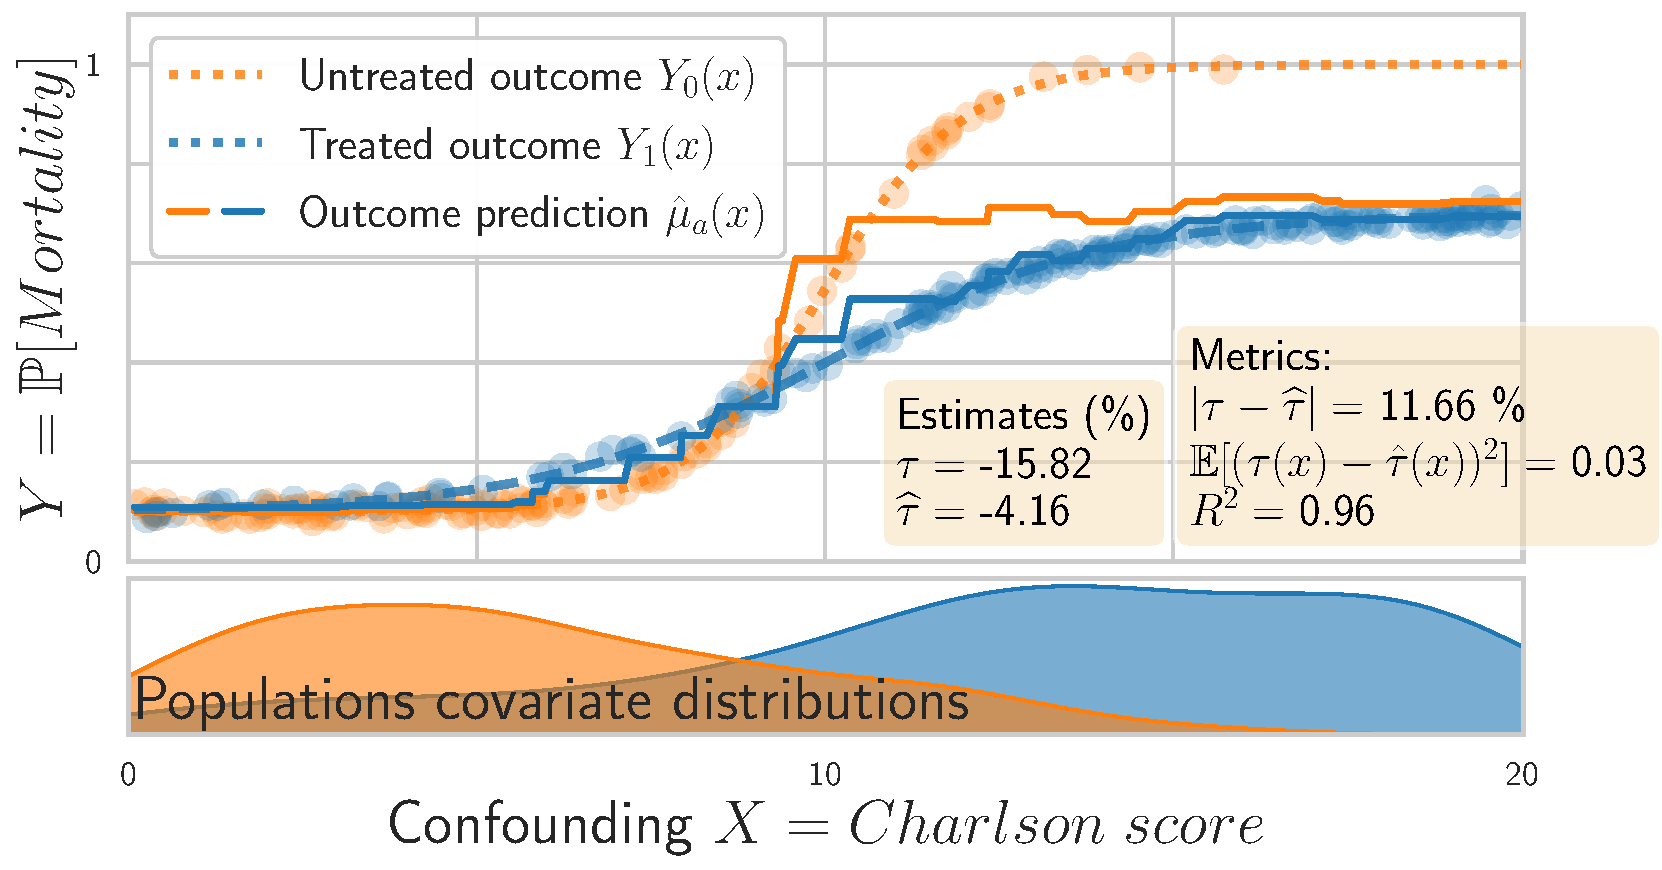
\includegraphics[width=1\linewidth]{toy_random_forest_high_R2_high_tau_risk.pdf}}%
            \put(7.05,4.4){\vector(0,1){.47}}
            \put(7.05,4.4){\vector(0,-1){.55}}
            \put(7.1,4.5){\scriptsize\sffamily treatment effect}
            \put(7.1,4.15){\small $\tau(x)$}
            \put(5.2,3.6){\small $\hat{\tau}(x)$}
            \put(5.15,3.6){\vector(0,1){.29}}
            \put(5.15,3.6){\vector(0,-1){.15}}
        \end{picture}

        {\sffamily\footnotesize\scalebox{0.95}{b) Linear model, worse average
            prediction but better causal inference}}

        \hfill%
        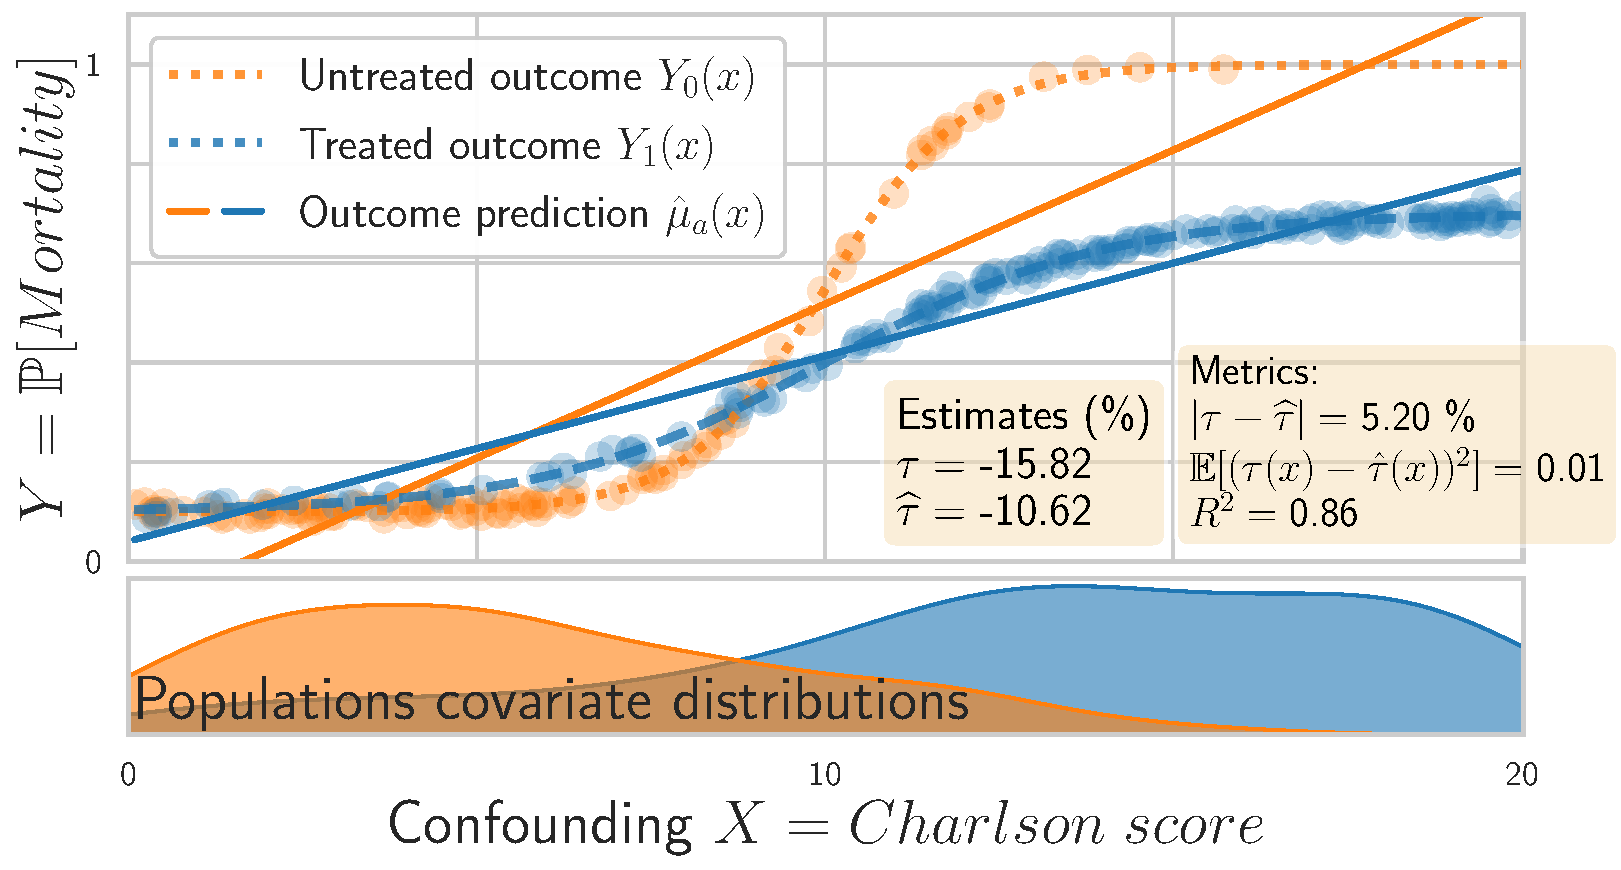
\includegraphics[width=1\linewidth]{toy_tlinear_model_small_R2_small_tau_risk.pdf}%
    \end{minipage}

    \caption[The best predictor may not estimate best causal
        effects]{\textbf{Illustration}: a) a random-forest predictor
        with high performance for standard prediction (high $R^2$) but that
        yields poor causal estimates (large error between true effect $\tau$ and
        estimated $\hat{\tau}$), b) a linear predictor with smaller
        prediction performance leading to better causal estimation. \\[1ex]
        Selecting the predictor with the smallest error to the individual
        treatment effect $\mathbb{E}[(\tau(x) - \hat{\tau}(x))^2]$
        --the $\tau\text{-risk}$, eq.\,\ref{eq:tau_risk} -- would lead to
        the best causal estimates; however computing this error is not
        feasible: it requires access to unknown quantities:
        $\tau(x)$. \\[1ex]
        While the random forest fits the data better than the linear model, it
        gives worse causal inference because its error is inhomogeneous between
        treated and untreated. The $R^2$ score does not capture this
        inhomogeneity.
        \label{fig:toy_example}
    }
\end{figure}


\subsection{Illustration: the best predictor may not estimate best causal
    effects}%

Using a predictor to reason on causal effects relies on contrasting the
prediction of the outcome for a given individual with and without the treatment.
%
Given various predictors of the outcome, which one should we use?
%
Standard predictive modeling or machine-learning practice selects the predictor
that minimizes the expected error on the outcome
\cite{poldrack2020establishment,varoquaux2022evaluating}. However, this
predictor may not be the best model to reason about causal effects of an
intervention as Figure \ref{fig:toy_example} illustrates. Consider the
probability $Y$ of an undesirable outcome (\eg death), a binary treatment $A \in
    \{0, 1\}$, and a covariate $X \in \mathbb R$ summarizing the patient health
status (\eg the Charlson index \cite{charlson_new_1987}). We simulate a
treatment beneficial (decreases mortality) for patients with high Charlson
scores (bad health status) but with little effect for patients in good condition
(low Charlson scores).


Figure \ref{fig:toy_example}a shows a random forest predictor with a
counter-intuitive behavior: it predicts well on average the outcome (as measured
by a regression $R^2$ score) but perform poorly to estimate causal quantities:
the average treatment effect $\tau$ (as visible via the error $|\tau -
    \hat{\tau}|$) or the conditional average treatment effect (the error
$\mathbb{E}[(\tau(x) - \hat{\tau}(x))^2]$, called CATE).
%
On the contrary, Figure \ref{fig:toy_example}b shows a linear model with
smaller $R^2$ score but better causal inference.%

The problem is that causal estimation requires controlling
an error on both treated and non-treated outcome for the same individual:
the observed outcome, and the non-observed \emph{counterfactual} one.
The linear model is misspecified --the outcome functions are not
linear--, leading to poor $R^2$; but it interpolates better to regions
where there are few untreated individuals --high Charlson score-- and
thus gives better causal estimates. Conversely, the random forest puts
weaker assumptions on the data, thus has higher $R^2$ score but is biased
by the treated population in the poor-overlap region, leading
to bad causal estimates.

This toy example illustrates that the classic minimum Mean Square Error
criterion is not suited to choosing a model among candidate
estimators for causal inference.

% A natural way to select a predictive model for causal inference would be

% an error measure between a causal quantity such as the CATE and models' estimate. But such error is
% not a ``feasible'' risk: it cannot be computed solely from observed data
% and requires oracle knowledge.

\section{Methods}\label{sec:framework}
\subsection{Neyman-Rubin Potential Outcomes framework}%
\label{sec:neyman_rubin}%

\paragraph{Settings}

The Neyman-Rubin Potential Outcomes framework
\cite{naimi2023defining,imbens_causal_2015} enables statistical reasoning on
causal treatment effects: Given an outcome $Y \in \mathbb R$ (\eg mortality risk
or hospitalization length), function of a binary treatment $A \in \mathcal{A} =
    \{0, 1\}$ (\eg~a medical procedure), and baseline
covariates $X \in \mathcal{X} \subset \mathbb{R}^d$, we observe the factual
distribution, $O = (Y(A), X, A) \sim \mathcal D = \mathbb P(y, x, a)$. However,
we want to model the existence of potential observations (unobserved ie.~counterfactual) that correspond to a different treatment. Thus we want
quantities on the counterfactual distribution $O^{*} = (Y(1), Y(0), X, A) \sim
    \mathcal D^{*} = \mathbb P(y(1), y(0), x, a)$.

Popular quantities of interest (estimands) are:
at the population level, the
Average Treatment Effect
\begin{flalign*}
    \text{ATE} &  &
    \tau \myeq \; \mathbb{E}_{Y(1),Y(0) \sim \mathcal D^*}[Y(1) - Y(0)];
               &  &
\end{flalign*}
at the individual level, to model heterogeneity, the Conditional Average Treatment Effect
\begin{flalign*}
    \text{CATE} &  &
    \tau (x) \myeq \; \mathbb{E}_{Y(1),Y(0) \sim \mathcal{D}^\star}[Y(1) - Y(0) | X=x].
                &  &
\end{flalign*}

\paragraph{Causal assumptions}

A given data needs to meet a few assumptions to enable identifying
causal estimands \cite{rubin_causal_2005}. The usual
\emph{strong ignorability} assumptions are  (details in
\ref{apd:causal_assumptions}): \emph{1)}
\emph{unconfoundedness} \mbox{$\{Y(0),
        Y(1) \} \indep A | X$}, \emph{~2)} \emph{strong overlap} ie. every patient has a
strictly positive probability to receive each treatment, \emph{3)}
\emph{consistency}, and \emph{4)} \emph{generalization}.

\paragraph{Estimating treatment effects with outcome models -- g-computation \cite{robins_new_1986}}\label{subsec:estimators}

Should we know the two expected outcomes for a given $X$,
we could compute the
difference between them, which gives the causal effect of the treatment.
%
These two expected outcomes can be estimated from observed data:
the consistency \ref{assumption:consistency} and unconfoundedness
\ref{assumption:ignorability} assumptions imply the following equality:
\begin{equation}\label{eq:mu_identification}
    \mathbb E_{Y(a) \sim \mathcal{D^{\star}}} [Y(a)|X=x] = \mathbb E_{Y \sim \mathcal{D}} [Y|X=x, A=a]
\end{equation}
On the left, the expectation is taken on the counterfactual unobserved
distribution. On the right, the expectation is taken on the factual observed
distribution conditionally on the treatment. For the rest of the
paper, the expectations will always be taken on the factual observed
distribution $\mathcal{D}$. This identification leads to outcome based estimators (ie.
g-computation estimators \cite{snowden_implementation_2011}):
\begin{eqnarray}
    \tau =& \mathbb E_{Y \sim \mathcal{D^{\star}}}[Y(1) - Y(0)|X=x]
    \notag
    \\
    = &\mathbb E_{Y \sim \mathcal{D}}[Y|A=1] - \mathbb E_{Y \sim \mathcal{D}}[Y| A=0]
    \label{eq:tau_population}
\end{eqnarray}
This equation builds on two quantities: the conditional expectancy
of the outcome given the covariates and either
treatment or no no treatment, called \emph{response function}:
\begin{flalign*}
    \text{Response function}
     &  &
    \mu_{a}(x) \myeq \; \mathbb E_{Y \sim \mathcal{D}} [Y|X=x, A=a]
     &  &
\end{flalign*}

Given a sample of data and the oracle response functions $\mu_0, \mu_1$, the
finite sum version of \autoref{eq:tau_population} leads to an
estimator of the ATE written:
\begin{equation}
    \hat \tau = \frac{1}{n} \biggl(\sum_{i=1}^n \mu_{1}(x_i) - \mu_{0}(x_i) \biggr)
    \label{eq:ate_estimate}
\end{equation}
This estimator is an oracle \emph{finite sum} estimator by opposition to the
population expression of $\tau$, $\mathbb{E}[\mu_{1}(x_i) - \mu_{0}(x_i)]
$,
which involves an expectation taken on the full
distribution $\mathcal D$, which is observable but requires infinite data. For
each estimator $\ell$ taking an expectation over $\mathcal D$, we use the symbol
$\hat \ell$ to note its finite sum version.

Similarly to the ATE, at the individual level, the CATE:
\begin{equation}
    \tau(x) = \mu_{1}(x) - \mu_{0}(x)
    \label{eq:cate_estimate}
\end{equation}

\paragraph{Robinson decomposition}
The \emph{R-decomposition}
of the outcome model\cite{robinson_rootnconsistent_1988} plays an important role:
introducing two quantities, the conditional mean outcome
and the probability to be treated (known as propensity score \cite{rosenbaum_central_1983}):
\begin{flalign}
    \text{Conditional mean outcome} &                    & m(x) \myeq \; & \mathbb E_{Y \sim
    \mathcal{D}} [Y|X=x]            &                    &
    \label{def:m}
    \\
    \text{Propensity score}         &                    &
    e(x) \myeq \;                   & \mathbb P[A=1|X=x]
    \label{def:propensity_score}
\end{flalign}
the outcome can be written
\begin{flalign}\label{eq:r_decomposition}
    \text{R-decomposition}            &  & y(a) = m(x) + \big( a - e(x) \big)
    \tau(x) + \varepsilon(x; a)\notag &  &
    \\\ &&\text{with}\quad \mathbb E[\varepsilon(X; A)|X, A] = 0&&
\end{flalign}
$m$ and $e$ are often called
\emph{nuisances} \cite{chernozhukov_double_2018}; they are unknown.

%As noted by \cite{johansson2022generalization}, the machine learning
%community often referred to the CATE by ITE, the Individual Treatment Effect.
%From a purely causal point of view, the ITE is uniquely defined for each
%individual and might not be accessible: $ITE(x_i) = Y_i(1) -  Y_i(0)$. On the
%contrary, the CATE can always be derived by taking conditional expectancies. It
%is the expected effect of the treatment in the region of the covariate space
%around X. %Too cultivate

\begin{table*}[bt!]
    \makebox[\textwidth]{
        \begin{threeparttable}[b]
            \caption{Review of causal risks
                ---
                The $R\text{-risk}^*$ is called $\tau \text{-risk}_R$ in
                \cite{schuler_comparison_2018}.
                \label{tab:evaluation_metrics}}
            \centering
            \begin{tabular}{llr}
                \toprule
                Risk                                                                                           & Equation
                                                                                                               & Reference                                                                                                                                           \\
                \midrule
                $\tau\text{-risk}=\text{MSE}(\tau(X), \tau_f(X))$                                              & $\mathbb E_{X\sim
                            p(X)}[(\tau(X) - \hat \tau_f(X))^2] $
                                                                                                               & Eq. \ref{eq:tau_risk} \cite{hill_bayesian_2011}                                                                                                     \\
                $\mu\text{-risk} = \text{MSE}(Y, f(X))$                                                        & $\mathbb{E}_{(Y, X, A)
                        \sim \mathcal D}\left[(Y-f(X ; A))^2 \right]$
                                                                                                               & Def. \ref{def:mu_risk} \cite{schuler_comparison_2018}                                                                                               \\
                $\mu\text{-risk}_{IPW}^*$                                                                      & $\mathbb{E}_{(Y, X, A)
                        \sim \mathcal D}\left[ \Big( \frac{A}{e(X)} + \frac{1-A}{1-e(X)} \Big)
                (Y-f(X ; A))^2 \right]$                                                                        & Def.
                \ref{def:mu_ipw_risk} \cite{vanderlaan_unified_2003}                                                                                                                                                                                                 \\
                $\tau\text{-risk}^{\star}_{IPW}$                                                               & $\mathbb{E}_{(Y, X, A) \sim \mathcal D} \left[ \Big(Y \left( \frac{A}{e(X)} - \frac{1-A}{1-e(X)}\right)-\hat \tau_f\left(X\right)\Big)^2 \right]$ &
                Def. \ref{def:tau_ipw_risk} \cite{wager_estimation_2018}
                \\
                $U\text{-risk}^*$                                                                              & $\mathbb{E}_{(Y, X, A) \sim \mathcal D}  \big[
                \big( \frac{Y-m\left(X\right)}{A-e\left(X\right)} -  \hat \tau_f\left(X\right)\big)^{2} \big]$ &
                Def. \ref{def:u_risk} \cite{nie_quasioracle_2017}
                \\
                $R\text{-risk}^*$                                                                              & $\mathbb{E}_{(Y, X, A)
                        \sim \mathcal D} \big[\big(\left(Y-m\left(X\right)\right)
                -\left(A-e\left(X\right)\right) \hat \tau_f\left(X\right)\big)^{2} \big]$                      &
                Def. \ref{def:r_risk} \cite{nie_quasioracle_2017}
                \\
                \bottomrule
            \end{tabular}
        \end{threeparttable}
    }
\end{table*}



\subsection{Model-selection risks, oracle and feasible}\label{sec:problem:model_selection}

\paragraph{Causal model selection}\label{sec:problem:causal_selection}

We formalize model selection for causal estimation. Thanks to the g-formula
identification (\autoref{eq:mu_identification}), a given outcome model $f: \mathcal X
    \times \mathcal A \rightarrow \mathcal{Y}$ --learned from data or built from
domain knowledge-- induces feasible estimates of the ATE and CATE (eqs
\ref{eq:ate_estimate} and \ref{eq:cate_estimate}), $\hat \tau_{f}$ and $\hat \tau_{f}(x)$.
%
Let $\mathcal F=\{f: \mathcal X \times \mathcal A \rightarrow \mathcal{Y}\}$ be
a family of such estimators. Our goal is to select the best candidate in this
family for the observed dataset $O$ using a risk
$\ell$:
\begin{equation}
    f^*_{\ell} = \argmin_{f \in \mathcal{F}} \ell(f, O)
    \label{eq:causal_model_selection}
\end{equation}

We now detail possible risks $\ell$, risks useful for causal
model selection, and how to compute them.


\paragraph{The $\tau\text{-risk}$: an oracle error risk}\label{paragraph:oracle_metrics}
%
As we would like to target the CATE, the following
evaluation risk is natural (also called PEHE \cite{schulam_reliable_2017, hill_bayesian_2011}):
\begin{flalign}\label{eq:tau_risk}
    \tau\text{-risk}(f) \myeq \mathbb E_{X\sim p(X)}[(\tau(X) - \hat \tau_f(X))^2]
\end{flalign}

Given observed data from $p(X)$, the expectation is computed with a
finite sum, as in eq.\,\ref{eq:ate_estimate}, to give an estimated
value $\widehat{\tau\text{-risk}}(f)$.
%
However this risk is not feasible as the oracles $\tau(x)$ are
not accessible with the observed data $(Y, X, A) \sim \mathcal D$.

\paragraph{Feasible error risks}\label{paragraph:feasible_metrics} Table
\ref{tab:evaluation_metrics} lists \emph{feasible} risks (Detailed in Appendix
\ref{def:feasible_risks}), based on the prediction error of the outcome model
and \emph{observable} quantities. These observable, called nuisances are $e$
--propensity score, eq \ref{def:propensity_score}-- and $m$ --conditional mean
outcome, eq \ref{def:m}. We give the definitions as \textit{semi-oracles},
function of the true unknown nuisances, but later instantiate them with
estimated nuisances, noted $\big(\check e, \check m \big)$. Semi-oracles risks
are superscripted with the $^{\star}$ symbol.

\subsection{Estimation and model selection procedure}\label{problem:estimation_procedure}

Causal model selection (eq
\ref{eq:causal_model_selection}) may involve estimating various quantities
from the observed data: the outcome model $f$, its induced risk as
introduce in the previous section, and possibly nuisances required by the
risk.
Given a dataset with $N$ samples, we split out a train and a test sets
$(\mathcal{T}, \mathcal{S})$. We
fit each candidate estimator $f \in \mathcal{F}$ on $\mathcal{T}$. We also fit
the nuisance models $(\check e, \check m)$ on the train set
$\mathcal{T}$, setting hyperparameters by a nested
cross-validation before fitting the nuisance estimators with these parameters
on the full train set. Causal quantities are then computed by applying the fitted  candidates
estimators $f \in \mathcal{F}$ on the test set $\mathcal{S}$. Finally, we
compute the model-selection metrics for
each candidate model on the test set. This procedure is described in Algorithm
\ref{problem:estimation_procedure:algo} and Figure
\ref{problem:estimation_procedure:figure}.

% As extreme inverse propensity weights induce high variance, clipping can be
% useful for numerical stability
% \cite{swaminathan_counterfactual_2015, ionides_truncated_2008}.

\begin{algorithm}[!htbp]
    \caption{Model selection procedure}\label{problem:estimation_procedure:algo} {%
        Given train and test sets $(\mathcal{T}, \mathcal{S}) \sim \mathcal{D}$,
        a candidate estimators $f$, a causal
        metrics $\ell$:
        \begin{enumerate}
            \item Prefit: Learn estimators for unknown nuisance quantities $(\check e,\,\check m)$ on the training set $\mathcal{T}$
            \item Fit: learn $\hat f(\cdot, a)$ on
                  $\mathcal T$
            \item Model selection: $\forall{x} \in \mathcal{S}$ predict
                  $\big(\hat f(x, 1), \hat f(x, 0)\big)$ and evaluate the estimator storing the metric value: $\ell(f, \mathcal S)$ -- possibly
                  function of $\check e$ and $\check m$
                  %\item Metric evaluation: return the oracle evaluation metrics
                  %evaluated on $\mathcal{S}$: $\big(\widehat{\tau\text{-risk}}(\hat
                  %f^*_{\ell}); \widehat{\ell}_{ATE}(\hat f^*_{\ell}) \big)$
        \end{enumerate}

    }
\end{algorithm}


\begin{figure}[h!]

    \centering\begin{minipage}{.95\linewidth}
        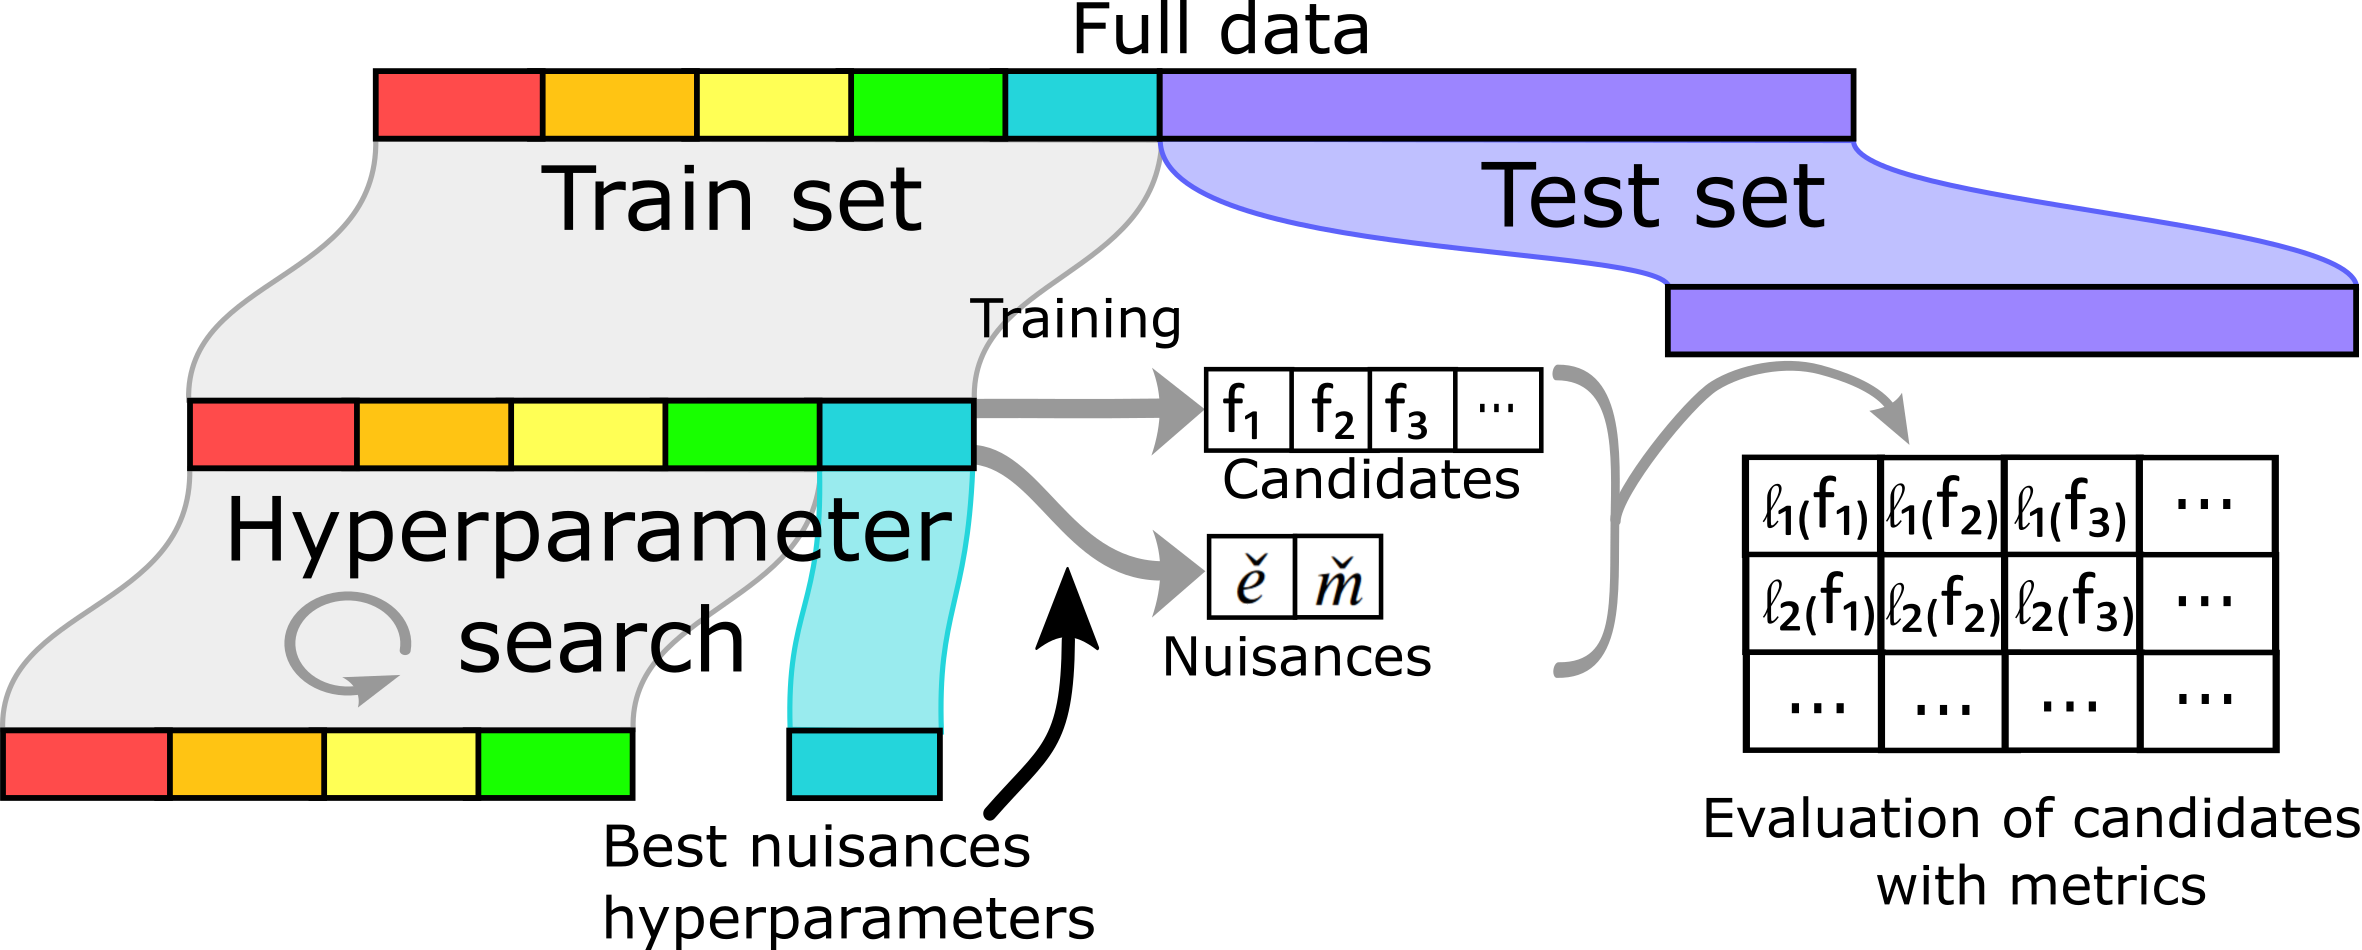
\includegraphics[width=\linewidth]{estimation_procedure_causal_selection_procedure.png}
    \end{minipage}
    \caption{Estimation procedure for causal model
        selection.}\label{problem:estimation_procedure:figure}
\end{figure}



\subsection{R-risk as reweighted oracle metric}\label{theory:r_risk_rewrite}

The $R\text{-risk}$ can be rewritten as a rebalanced $\tau \text{-risk}$.

% We now one feasible risks, $\mu \text{-risk}_{IPW}$ and the
% $R\text{-risk}$ to the oracle $\tau\text{-risk}$. Both results make
% explicit the role of overlap for the performances of causal risks.

This rewriting involves reweighted residuals: for each potential outcome, $a \in
    \{0; 1\}$, the variance conditionally on $x$ is \cite{shalit_estimating_2017}:
\begin{equation*}\label{eq:residuals}
    \sigma_{y}^{2}(x ; a) \overset{\text{def}}{=}
    \int_{y}\left(y-\mu_{a}(x)\right)^{2} p(y \mid x=x ; A=a) \, d y
\end{equation*}
Integrating over the population, we get the Bayes squared error:
$\sigma^2_{B}(a) = \int_{\mathcal X} \sigma_y^2(x;a) p(x)dx$
and its propensity weighted version:
$\tilde{\sigma}^2_{B}(a) = \int_{\mathcal X}\sigma_y^2(x;a)\,  p(x;
    a)\,dx$. In case of a purely deterministic link between the
covariates, the treatment, and the outcome, these residual terms are null.

%\md{Lower bound: I think that there is no lower bound of the tau-risk with the
%mu-risk. That means that we can have a mu risk of 0 wheras the taurisk is
%non-null. Todo for myself: develop an example with overfitted 1NN on the
%observed data.}


\begin{proposition}[$R \text{-risk}$ as reweighted
        $\tau\text{-risk}$]\label{theory:prop:r_risk_rewrite} Given an outcome model
    $f$, its $R\text{-risk}$ appears as weighted version of its $\tau\text{-risk}$
    (Proof in \ref{apd:proofs:r_risk_rewrite}):
    \begin{align}
        R\text{-risk}^*(f) & = \int_{x} e(x)\big(1-e(x)\big)\big(\tau(x)-\tau_ {f}(x)\big)^{2} p(x) d x \nonumber \\
                           & \quad\; + \tilde{\sigma}_B^2(1) + \tilde{\sigma}_B^{2}(0)
    \end{align}
\end{proposition}

The $R \text{-risk}$ targets the oracle at the cost of an overlap re-weighting
and the addition of the reweighted Bayes residuals, which are independent of
$f$. In good overlap regions the weights $e(x) \big(1-e(x) \big)$ are close to
$\frac{1}{4}$, hence the $R \text{-risk}$ is close to the desired gold-standard
$\tau \text{-risk}$. For randomized control trials, this weight is constant
making the $R\text{-risk}$ particularly suited for exploring
heterogeneity (Appendix \ref{apd:theory:special_cases})



\section{Empirical Study}\label{sec:empirical_study}

%We now explore empirically the behavior of these different causal selection
%metrics.
%\subsection{Causal metrics under evaluation}

We evaluate the following causal metrics, oracle and feasible
versions, presented in Table
\ref{tab:evaluation_metrics}:\\
$\widehat{\mu\text{-risk}}_{IPW}^*$,
$\widehat{R\text{-risk}}^*$,
$\widehat{U\text{-risk}}^*$,
$\widehat{\tau\text{-risk}_{IPW}}^*$,
$\widehat{\mu\text{-risk}}$,
$\widehat{\mu\text{-risk}}_{IPW}$,
$\widehat{R\text{-risk}}$,
$\widehat{U\text{-risk}}$,
$\widehat{\tau\text{-risk}_{IPW}}$.
We benchmark the metrics in a variety of settings:
many different simulated data generation
processes and three semi-simulated datasets \footnote{Scripts for the simulations and the selection procedure are available at
    \url{https://github.com/soda-inria/caussim}.
}.

\subsection{Caussim: Extensive simulation settings}\label{subsec:simulations}

\paragraph{Data Generation}

We use simulated data, on which the ground-truth causal effect is known. Going
beyond prior empirical studies of causal model selection
\cite{schuler_comparison_2018,alaa_validating_2019}, we use many
generative processes, which is needed to reach general conclusions (Appendix \ref{apd:results:seed_effect}).

We generate the response functions using random bases extension, a common method
in biostatistics, \eg functional regression with splines
\cite{howe_splines_2011, perperoglou_review_2019}. By allowing the function to
vary at specific knots, we control the complexity of the non-linear outcome
models. We use random approximation of Radial Basis Function (RBF) kernels
\cite{rahimi_random_2008} to generate the outcome and treatment functions. RBF
use the same process as polynomial splines but replace polynomial by Gaussian
kernels. Unlike polynomial, Gaussian kernels have decreasing influences in the
input space. This avoids unrealistic divergences of the functions at the
ends of the feature space. We generate 1\,000 datasets based on these functions,
with random overlap parameters. Example shown in Figure
\ref{fig:simulation_examples} and details in \ref{apd:experiments:generation}.

\captionsetup[sub]{font=large,labelfont={bf,sf}}%

\paragraph{Family of candidate estimators}

We test model selection across different candidate estimators that
approximate imperfectly the
data-generating process. To build such estimators, we first use a RBF
expansion similar to that used for data generation. We choose two random
knots and transform the raw data features with a Gaussian
kernel. This step is referred as the featurization. Then, we fit a linear
regression on these transformed features. We consider two ways of combining
these steps for outcome model; we use common nomenclature
\cite{kunzel_metalearners_2019,shen2023rctrep} to refer to these different
meta-learners that differ on how they model, jointly or not, the treated and the
non treated:
\begin{itemize}
    \item SLearner: A single learner for both population, taking the treatment as
          a supplementary covariate.
    \item SftLearner: A single set of basis functions is sampled at random for both
          populations, leading to a given feature space used to model both the treated and
          controls, then two
          separate different regressors are fitted on this shared representation.
    \item TLearner: Two completely different learners for each population, hence
          separate feature representations and regressors.
\end{itemize}

% We do not include more elaborated meta-learners such as R-learner
% \cite{nie_quasioracle_2017} or X-learner
% \cite{kunzel_metalearners_2019}. Our goal is not to have the best possible
% learner but to have a variety of sub-optimal learners to compare the
% different causal metrics. For the same reason, we did not include more powerful
% outcome models such as random forests or boosting trees.

For the regression step, we fit a Ridge regression on the transformed features
with 6 different choices of the regularization parameter $\lambda \in [10^{-3},
        10^{-2}, 10^{-1}, 1, 10^{1}, 10^{2}]$, coupled with a TLearner or
a SftLearner.
We sample 10 different random basis for learning and
featurization yielding a family $\mathcal F$ of 120 candidate estimators.
%

\subsection{Semi-simulated datasets}

\paragraph{Datasets}\label{semi_simulated:datasets}

We also use three semi-simulated
data adding a known synthetic causal effect to real --non synthetic-- healthcare
covariate. ACIC 2016 \cite{dorie_automated_2019} is based on the Collaborative
Perinatal Project \cite{niswander_women_1972}, a RCT studying infants’
developmental disorders containing 4,802 indivduals and 55 features. We used 770
dataset instances: 10 random seeds for each of the 77 simulated settings for the
treatment and outcomes.  ACIC 2018 \cite{shimoni_benchmarking_2018} simulated
treatment and outcomes for the Linked Births and Infant Deaths Database (LBIDD)
\cite{macdorman_infant_1998} with $D=177$ covariates. We used all 432 datasets
of size $N=5\,000$.  Twins \cite{louizos_causal_2017} is an augmentation of real
data on twin births and mortality rates \cite{almond_costs_2005}. There are
$N=11\,984$ samples, and $D=50$ covariates for which we simulated 1,000
different treatment allocations. Appendix
\ref{apd:experiments:datasets} gives datasets details.


\paragraph{Family of candidate
    estimators}\label{semi_simulated:candidate_estimators}

For these three datasets, the family of candidate estimators are gradient
boosting trees for both the response surfaces and the treatment
\footnote{Scikit-learn regressor,
    \href{https://scikit-learn.org/stable/modules/generated/sklearn.ensemble.HistGradientBoostingRegressor.html}{HistGradientBoostingRegressor},
    and classifier,
    \href{https://scikit-learn.org/stable/modules/generated/sklearn.ensemble.HistGradientBoostingClassifier.html}{HistGradientBoostingClassifier}.}
with S-learner, learning rate
in $\{0.01, 0.1, 1\}$, and maximum number of leaf nodes in $\{25, 27, 30, 32,
    35, 40\}$ resulting in a family of size 18.

\paragraph{Nuisance estimators}

Drawing from the TMLE literature that uses combination of flexible
machine learning methods \cite{schuler_targeted_2017}, we model the nuisances
$\check e$ (respectivley $\check m$) with a meta-learner: a stacked estimator of ridge
and boosting classifiers (respectively regressions) (hyperparameter selection in Appendix \ref{apd:experiments:nuisances_hp}).


\subsection{Measuring overlap between treated and non treated}\label{subsec:measuring_overlap}

%\idea{Overlap is important but not easily measurable}
Good overlap between treated and control population is crucial for causal
inference (Assumption \ref{assumption:overlap}). We introduce the
Normalized Total Variation (NTV), a divergence based on the propensity score
summarizing the overlap between both populations (Appendix
\ref{apd:motivation_ntv}).

\begin{figure}[!b]
    % XXX: for submission
    \centering\begin{minipage}{\linewidth}
        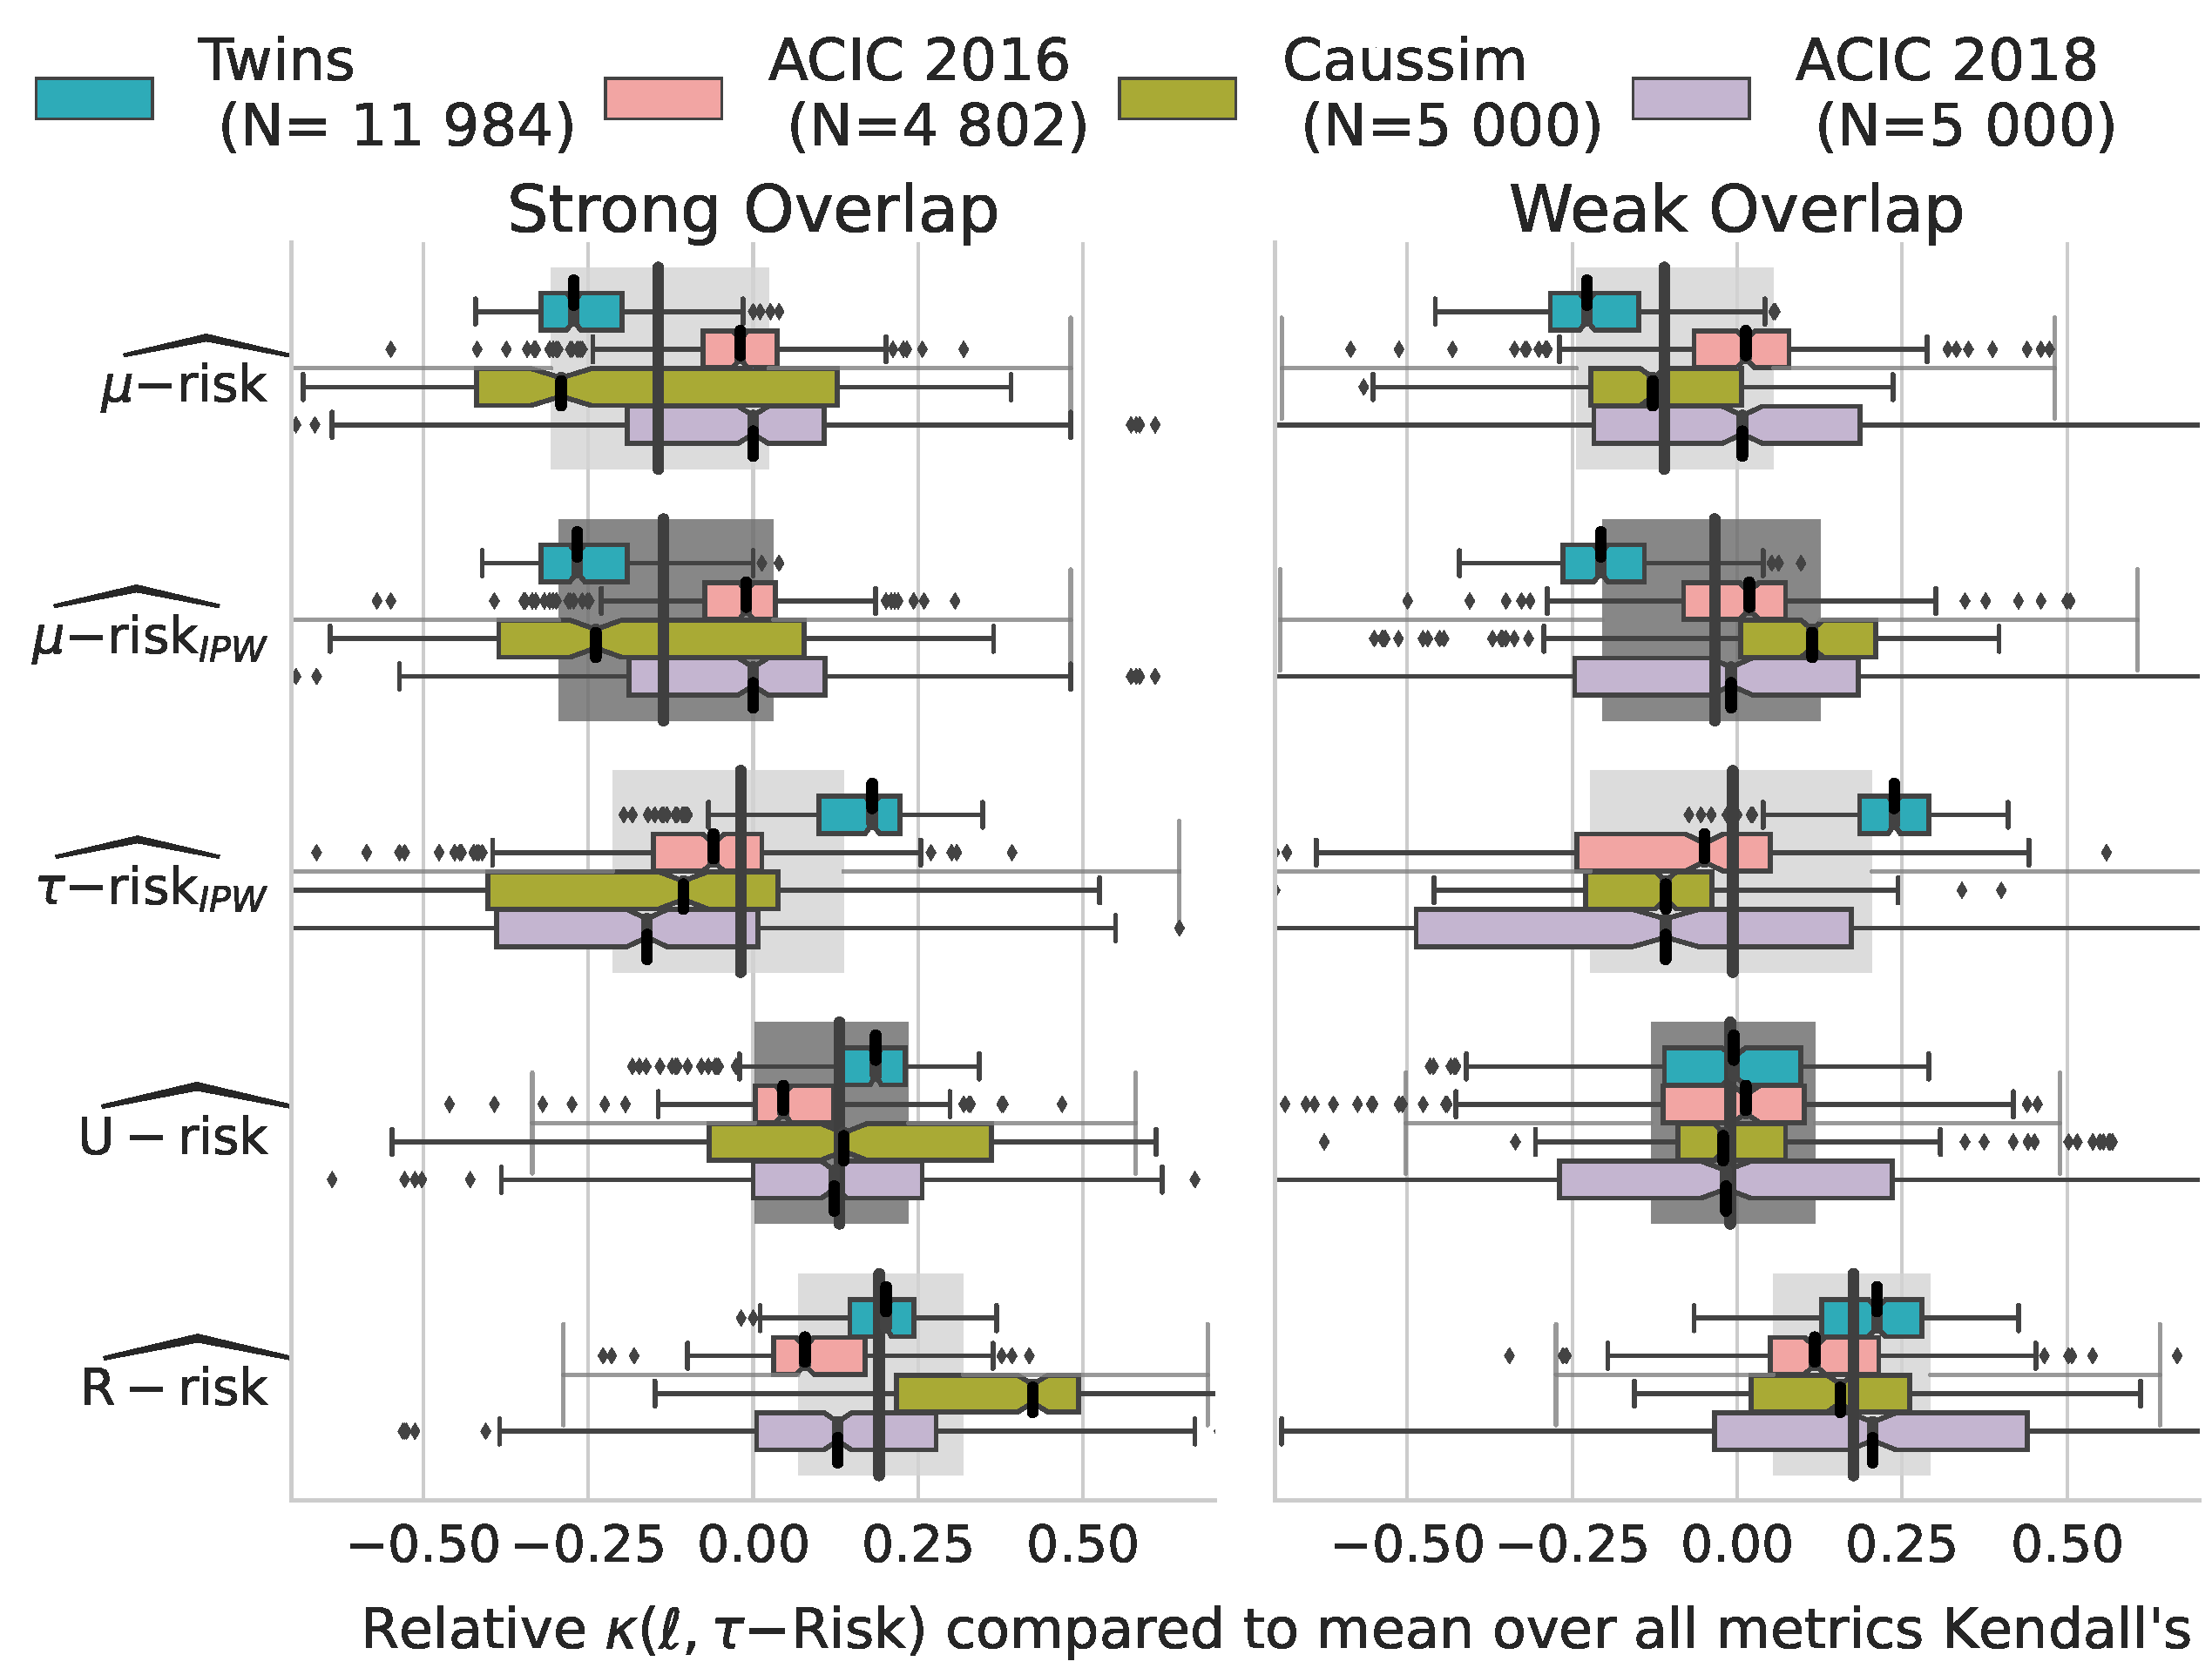
\includegraphics[width=\linewidth]{_1_r_risk_domination_r_risk_domination__ref_metric_mean_risks_by_Dataset_feasible_only.pdf}
    \end{minipage}
    \caption{\textbf{The $R$-risk is the best metric}: Relative Kendall's $\tau$ agreement with $\tau\text{-risk}$.
        Strong and Weak overlap correspond to the first and last tertiles of the overlap distribution measured with
        Normalized Total Variation eq. \ref{eq:ntv}. \ref{apd:experiments:additional_results} presents the same results
        by adding semi-oracle risks in Figure \ref{apd:fig:relative_kendalls_all_datasets_all_metrics}, measured with
        absolute Kendall's in Figure \ref{apd:fig:all_datasets_tau_risk_ranking_agreement} and with $\tau\mathrm{-risk}$
        gains in Figure \ref{apd:all_datasets_normalized_bias_tau_risk_to_best_method}. Table
        \ref{apd:table:relative_kendalls_all_datasets} gives median and
        IQR of the relative Kendall.}\label{fig:relative_kendalls_all_datasets}
\end{figure}



\section{Results: factors driving good model selection}\label{empirical_study:results}


\paragraph{The $R\text{-risk}$ is the best metric}

Figure \ref{fig:relative_kendalls_all_datasets} shows the agreement between the
ideal ranking of outcome models given the oracle $\tau\text{-risk}$ and the different
feasible causal metrics. We measure this agreement with relative\footnote{To
    remove the variance across datasets (some datasets lead to easier model
    selection than others), we report values for one metric relative to the mean of
    all metrics for a given dataset instance: $\text{Relative} \,
        \kappa(\ell,\tau\mathrm{{-risk}})= \kappa(\ell,\tau\mathrm{{-risk}}) -
        mean_{\ell}\big(\kappa(\ell,\tau\mathrm{{-risk}})\big)$} Kendall tau $\kappa$
(eq. \ref{eq:kendall_tau}) \cite{kendall_new_1938}. Given the importance of
overlap in how well metrics approximate the oracle $\tau\text{-risk}$, we
separate strong and weak overlap.

Among all metrics, the classical mean squared error (ie. factual
$\mu\text{-risk}$) is worse and reweighting it with propensity score
($\mu\text{-risk}_{IPW}$) does not bring much improvements. The
$R\text{-risk}$, which includes a model of mean outcome and propensity
scores, leads to the best performances. Interestingly, the
$U\text{-risk}$, which uses the same nuisances, deteriorates in weak overlap, probably due to variance
inflation when dividing by extreme propensity scores.

Beyond rankings, the differences in terms of absolute
ability to select the best model are large: The R-risk selects a model
with a $\tau\text{-risk}$ only 1\% higher
than the best
possible candidate for strong overlap on Caussim, but selecting with
the $\mu\text{-risk}$ or $\mu\text{-risk}_{IPW}$ --as per machine-learning
practice-- leads to 10\% excess risk and using $\tau\text{-risk}_{IPW}$
--as in some causal-inference methods \cite{athey2016recursive,gutierrez_causal_2016}--leads to 100\% excess risk
(Figure
\ref{apd:all_datasets_normalized_bias_tau_risk_to_best_method}). Across
datasets, the $R\text{-risk}$ consistently decreases the
risk compared to the $\mu\text{-risk}$: from
0.1\% to 1\% on ACIC2016,  1\% from to 20\% on ACIC2018,
and 0.05\% from to 1\% on Twins.


\paragraph{Model selection is harder for low population
    overlap}

Model selection for causal inference becomes more and more difficult with
increasingly different treated and control populations (Figure
\ref{fig:all_datasets_overlap_effect_r_risk}). The absolute Kendall's
coefficient correlation with $\tau\text{-risk}$ drops from 0.9
(excellent agreement with oracle selection) to 0.6 on both Caussim and ACIC 2018
(\ref{apd:experiments:additional_results}).

\begin{figure}[!h]
    % XXX: for submission
    \centering\begin{minipage}{\linewidth}
        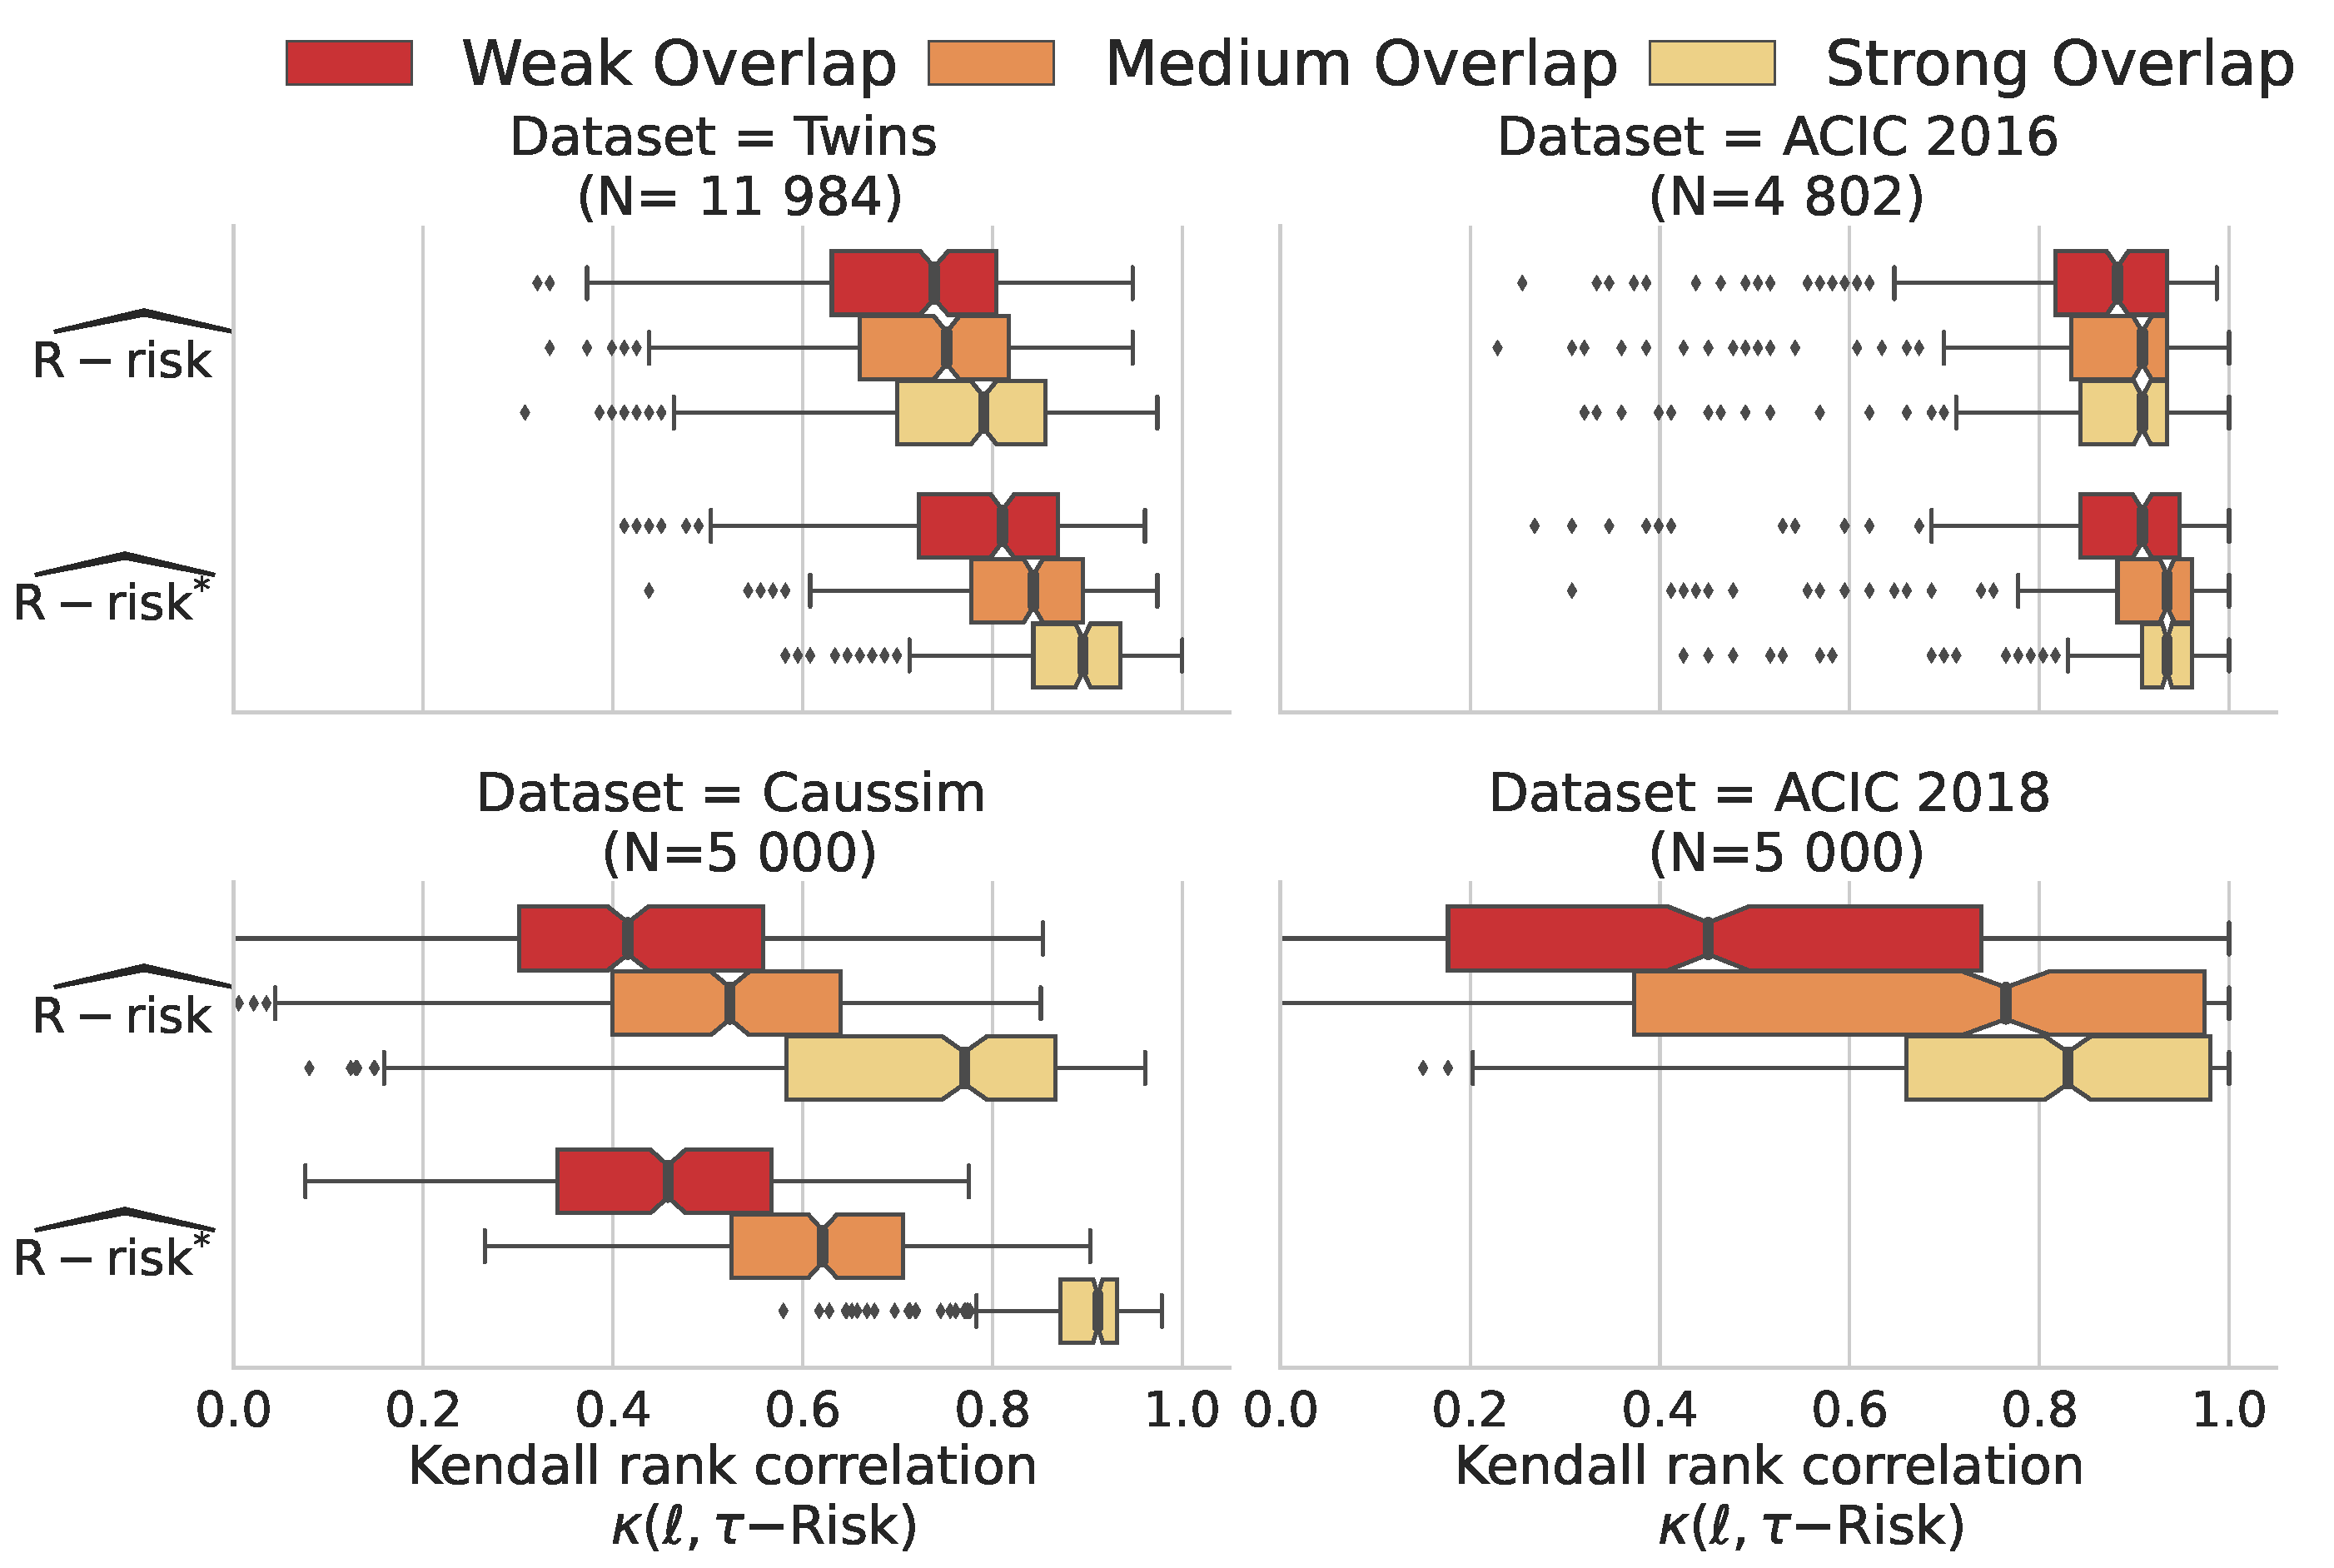
\includegraphics[width=\linewidth]{_2_overlap_influence_overlap_by_bin_comparaison_kendall_by_Dataset_r_risk_only_twocols.pdf}
    \end{minipage}
    \caption{\textbf{Model selection is harder for low population
            overlap}:
        Kendall's $\tau$ agreement with $\tau\text{-risk}$. Strong, medium and Weak overlap
        are the tertiles of the overlap measured with NTV eq. \ref{eq:ntv}. \ref{apd:experiments:additional_results} presents results for all
        metrics in Figure \ref{apd:fig:all_datasets_overlap_effect} in absolute
        Kendall's and continuous overlap values in Figure
            {\ref{apd:fig:all_datasets_tau_risk_ranking_agreement}}.}\label{fig:all_datasets_overlap_effect_r_risk}
\end{figure}



\paragraph{Nuisances can be estimated on the same data as outcome models}

Using the train set $\mathcal{T}$ both to fit the candidate estimator and the
nuisance estimates is a form of double dipping which can lead errors in
nuisances correlated to that of outcome models
\cite{nie_quasioracle_2017}. In theory, these correlations can bias model
selection and, strictly speaking, push
to split out a third separated data set --a ``nuisance set''-- to fit the
nuisance models. The drawback is that it depletes the data available for
model estimation and selection. However, Figure
\ref{fig:procedures_comparison} shows no substantial difference between a procedure with a separated
nuisance set and the simpler shared nuisance-candidate set procedure.

Empirically, the best split is 90\,\%/10\,\%:
using 90\,\% of the data
to estimate both the nuisances and candidates, then computing the risks on the
remaining test set for model selection (experiments in Appendix
\ref{apd:results:data_split}).

\begin{figure}[!tb]
    % XXX: for submission
    \centering\begin{minipage}{\linewidth}
        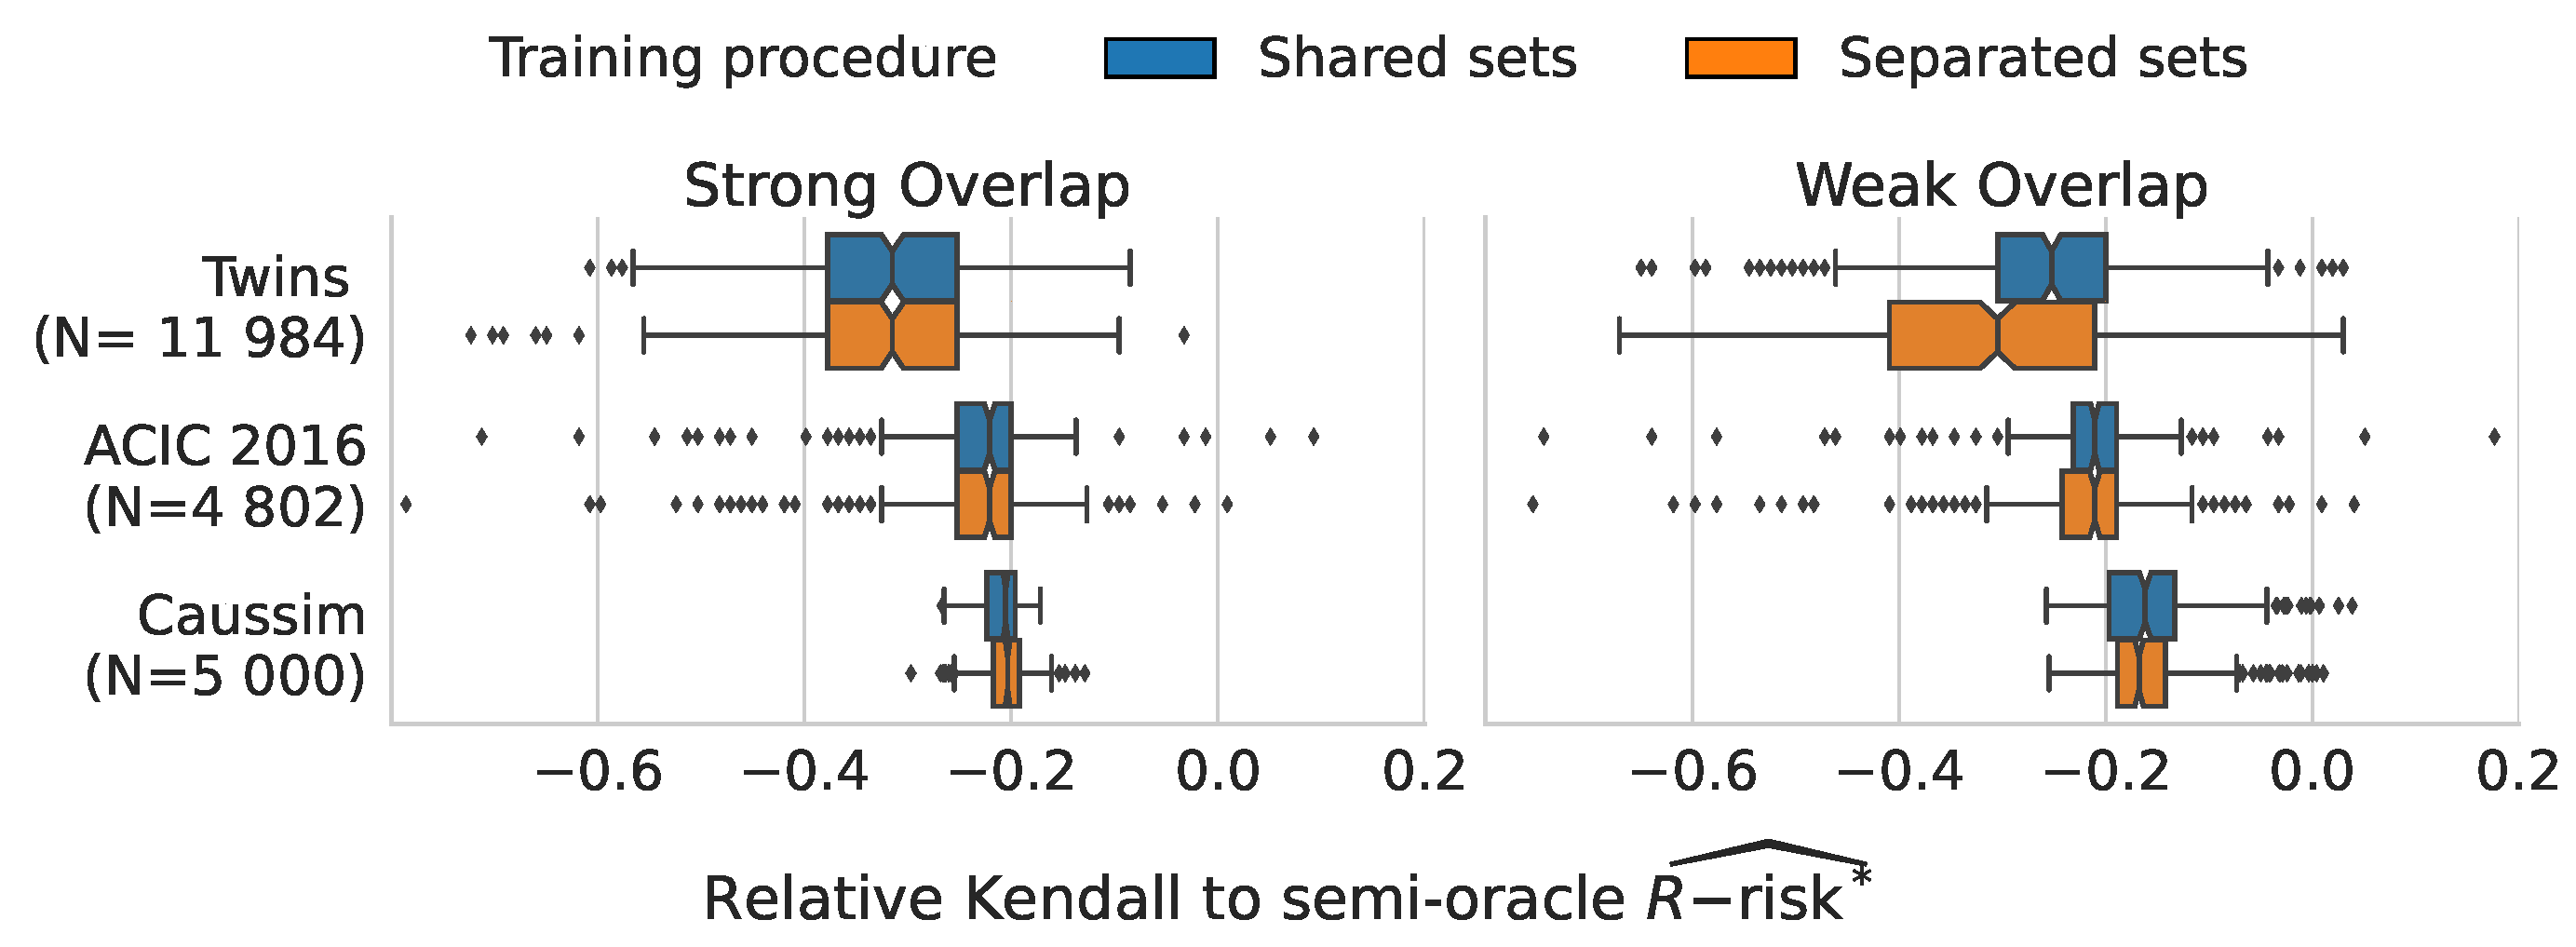
\includegraphics[width=\linewidth]{_3_procedure_r_risk_only_3datasets_twocols.pdf}
    \end{minipage}

    \caption{\textbf{Nuisances can be estimated on the same data as outcome
            models}: Results for the R-risk are similar between the
        \textcolor{MidnightBlue}{shared
            nuisances/candidate set} and
        the \textcolor{RedOrange}{separated nuisances set} procedures. Figure
        \ref{apd:fig:procedures_comparison_all_metrics} details results for all metrics.}\label{fig:procedures_comparison}
\end{figure}

\paragraph{Stacked models are good overall estimators of nuisances}

Stacked nuisances estimators (boosting and linear) lead to feasible
metrics with close performances to the oracles ones: the
corresponding estimators recover well-enough the true nuisances.
One may wonder if simpler models for the nuisance could be useful,
in particular in data-poor settings or when the true models are linear.
Figure \ref{fig:all_datasets_nuisances_comparison} compares causal model
selection estimating nuisances with stacked estimators or linear model.
It comprises the Twins data, where the true propensity model is linear,
and a downsampled version of this data, to study a situation favorable to
linear models. In these settings,
stacked and linear estimations of the nuisances performs equivalently.
Detailed analysis (Figure \ref{apd:fig:nuisances_comparison_twins})
confirms that using adaptive models --as built by
stacking linear models and gradient-boosted trees-- suffices to estimate nuisance.

\begin{figure}[!tb]
    % XXX: for submission
    \centering\begin{minipage}{\linewidth}
        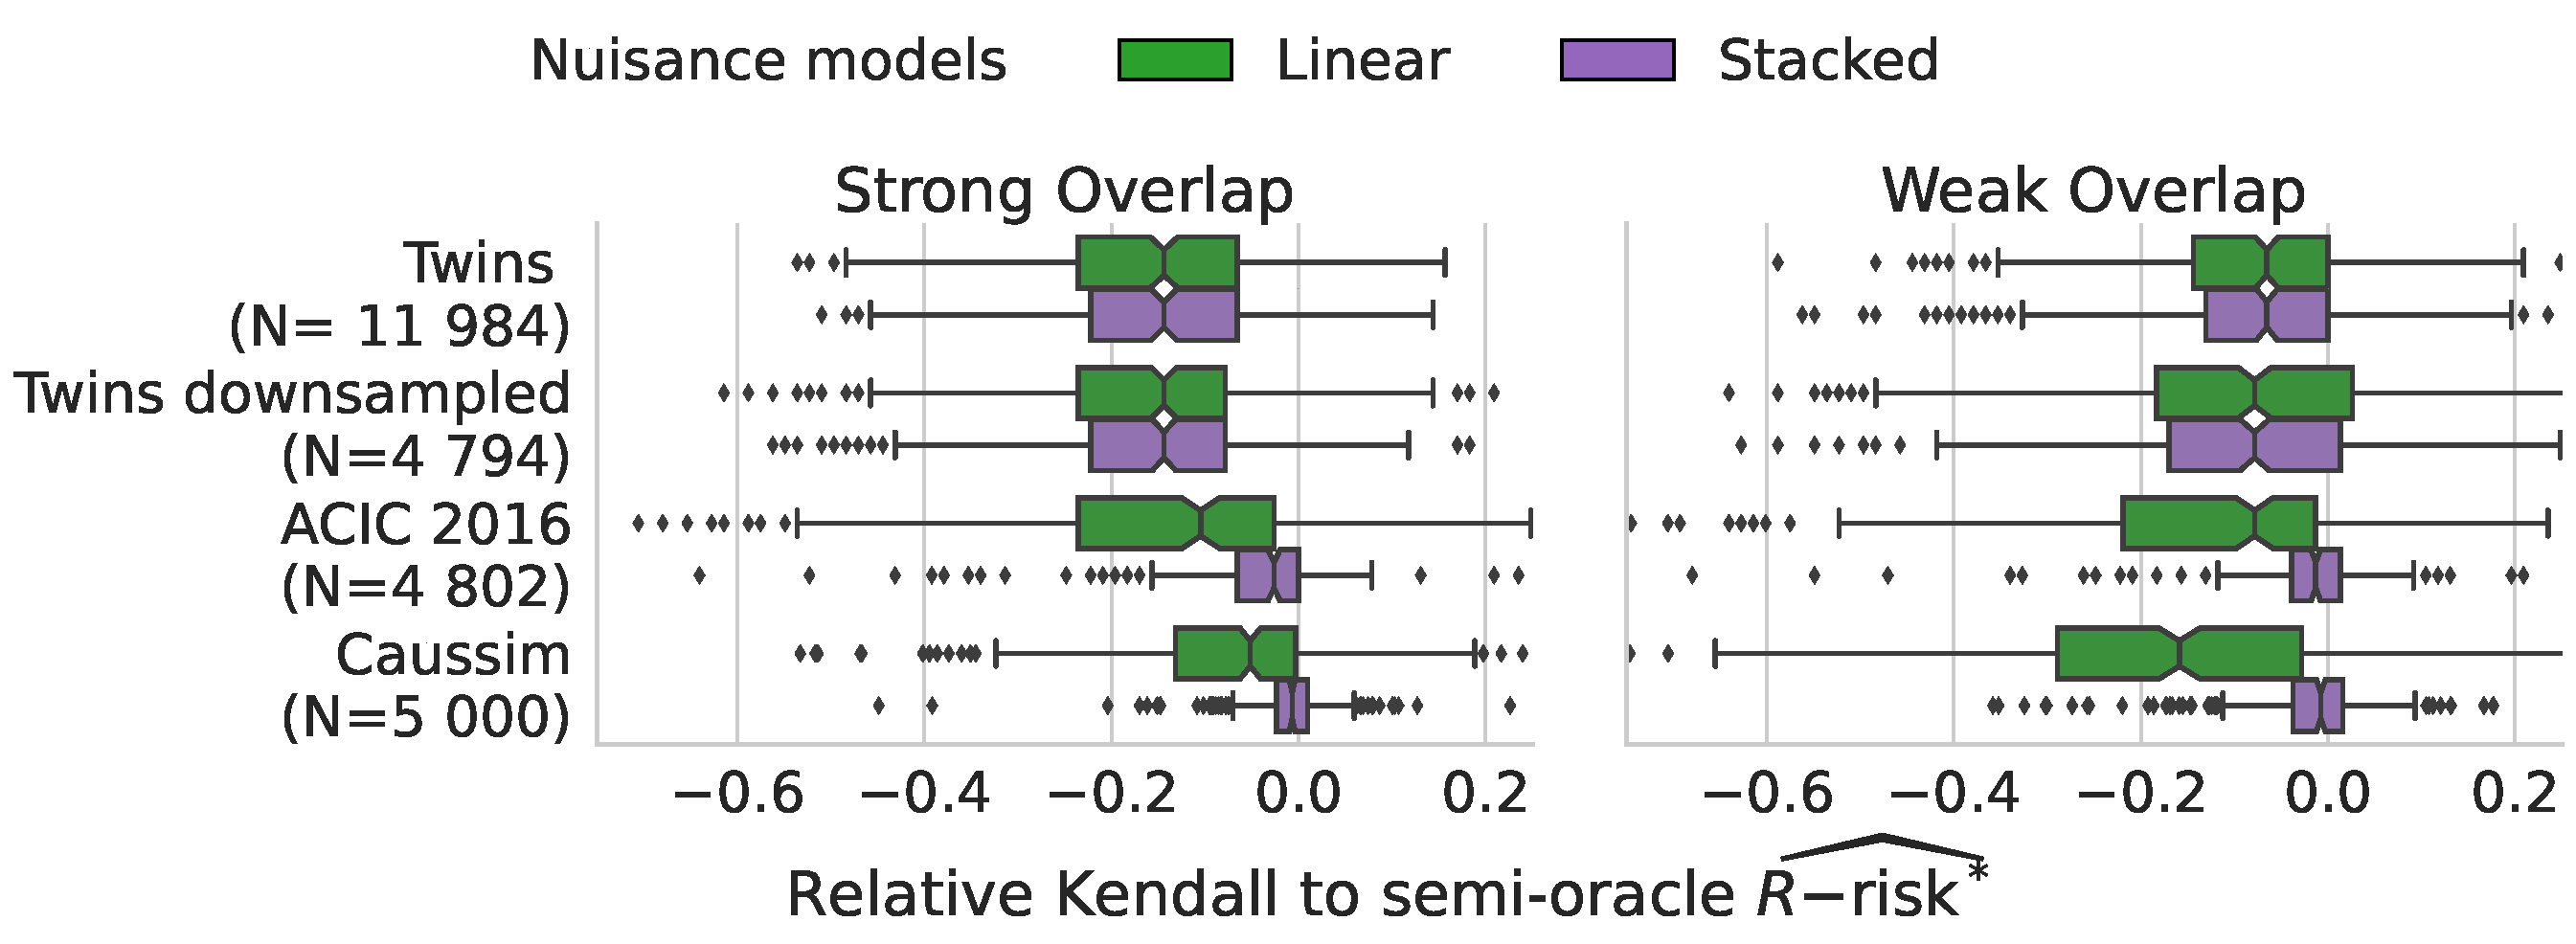
\includegraphics[width=\linewidth]{_4_nuisance_models_r_risk_only_3datasets_twocols.pdf}
    \end{minipage}

    \caption{\textbf{\textcolor{DarkOrchid}{Stacked
                models} are good overall estimators of the nuisances}:
        Results are shown only for the
        R-risk; Figure \ref{apd:fig:nuisances_comparison}
        details every metrics. For Twins, where the true propensity
        model is linear, \textcolor{DarkOrchid}{stacked} and
        \textcolor{ForestGreen}{linear}
        estimations of the nuisances performs equivalently, even for a downsampled version
        (N=4,794). }\label{fig:all_datasets_nuisances_comparison}
\end{figure}




\section{Discussion and conclusion}\label{sec:discussion}\label{sec:conclusion}


\paragraph{Nuisance models: more gain than pain}
%
Predictive models are increasingly used to reason about treatment effects, for
instance in precision medicine to drive individualized decision. Our results
highlight that they should be selected, validated, and tuned using different
procedures and error measures than those classically used to assess prediction. Rather, selecting the best outcome
model according to the $R\text{-risk}$ (eq.\, Definition \ref{def:r_risk}) leads
to more valid causal estimates. Estimating the $R\text{-risk}$ requires a more
complex procedure than standard cross-validation used \eg in machine
learning: it involves fitting nuisance models necessary for model
evaluation.
Our results show that these can be learned on the same set of data as the
outcome models evaluated. The nuisance models must be well estimated (Figure
\ref{fig:all_datasets_nuisances_comparison}). Our results show that using for
nuisance models a flexible stacking-based family of estimator suffices for good
model selection. To select propensity score models, we used the Brier score,
minimized by the true individual probability. An easy mistake is to
use calibration errors popular in machine learning
\cite{platt_probabilistic_1999,zadrozny_obtaining_2001,niculescu-mizil_predicting_2005,minderer_revisiting_2021}
as these select not for the individual posterior probability but for an
aggregate error rate \cite{perez2022beyond}.


%
% However these models are easier to select and control than a causally-valid
% outcome model, as they are associated to errors on observed distributions. 
% In fact, a feasible $R\text{-risk}$ --where the nuisances
% are estimated-- performs almost as well as an oracle $R\text{-risk}$ --where the
% nuisances are known. This may be explained by
% results that suggest that estimation errors on both
% nuisances partly compensate out in the
% $R\text{-risk}$ \cite{daniel2018double,kennedy2020optimal,nie_quasioracle_2017,chernozhukov_double_2018,zivich2021machine,naimi2021challenges}.


%\paragraph{Extension to binary outcomes}
%While we focused on continuous outcomes, in medicine, the target outcome
%is often a categorical variable such as mortality status or diagnosis. In
%this case, it may be interesting to focus on other estimands than the
%Average Treatment Effect $\mathbb{E}[Y(1)] -\mathbb{E}[Y(0)] $, for instance the relative risk
%$\frac{\mathbb P(Y(1) = 1)}{\mathbb P(Y(0) = 1)}$
%or the odd ratio, $\frac{\mathbb P(Y(1) = 1) / [1 - \mathbb P(Y(1)
%    =1)]}{\mathbb P(Y(0) = 1) / [1 - \mathbb P(Y(0) = 1]}$ are often used
%\cite{austin2017estimating}. While the odds ratio is natural for
%case-control studies \cite{rothman2008case}, other measures
%can reduce heterogeneity \cite{colnet2023risk}.
%In the log domain, the ratios are written as a difference, the
%framework studied here can directly apply.
%% In particular, the log odds ratio is estimated by the common
%% cross-entropy loss (or log loss) as in logistic regression.

\paragraph{More $R\text{-risk}$ to select models driving decisions}

Increasingly complex prediction models integrating richer medical data
have flourished because their predictions can be easily
demonstrated and validated on left-out data. But using them to underpin a
decision on whether to treat or not requires more careful validation,
using a metric accounting for the
putative intervention, the $R\text{-risk}$. The $R\text{-risk}$
brings a sizeable benefit to select the most adequate model, even when
model development is based on treated and
untreated population with little differences, as in RCTs. To facilitate better model selection, we provide Python
code\footnote{\url{https://github.com/soda-inria/causal_model_selection}}.
% Using the $R\text{-risk}$ does make evaluation more
% complicated not only because the procedure is more involved, but also
% because each intervention requires a dedicated evaluation. However, such
% off-policy evaluation remains much less costly than the recommended good
% practice of impact evaluation testing the ability of a prediction model
% to actually guide patient health \cite{hendriksen2013diagnostic}. Also,
This model-selection procedure puts no constraints on the models used to
build predictive models: it opens the door to evaluating a wide range of
models, from gradient boosting to convolutional neutral, or language
models.

\clearpage


\onecolumn

\renewcommand\thefigure{S\arabic{figure}}
\renewcommand\thetable{S\arabic{table}}
\setcounter{figure}{0}
\setcounter{table}{0}

%%%%%%%%%%%%%%

\begin{appendices}

    %\part*{Supplementary materials:\\How to select predictive models for decision-making or causal inference? }

    \setcounter{secnumdepth}{3}

    %\part{Supplementary materials}

    %The following supporting information is available as part of the online article:

    \section{Variability of ATE estimation on ACIC
      2016}\label{apd:toy_example:acic_2016_ate_variability}

    Figure \ref{fig:acic_2016_ate_heterogeneity} shows ATE estimations for six
    different models used in g-computation estimators on the 76 configurations of
    the ACIC 2016 dataset. Outcome models are fitted on half of the data and
    inference is done on the other half --ie. train/test with a split ratio of 0.5.
    For each configuration, and each model, this train test split was repeated ten
    times, yielding non parametric variance estimates
    \cite{bouthillier_accounting_2021}. Figure \ref{fig:acic_2016_ate_heterogeneity}
    shows large variations obtained across different outcome estimators on
    semi-synthetic datasets \cite{dorie_automated_2019}. Flexible models such as
    random forests are doing well in most settings except when treated and untreated
    populations differ noticeably, in which case a linear model (ridge) is to be
    preferred. However random forests with different hyper-parameters (max depth= 2)
    yield poor estimates. A simple rule of thumb such as preferring flexible models
    does not work in general; model selection is needed.

    %\idea{It is crucial to have tools for model selection.}

    \begin{figure}[!b]
        \centering
        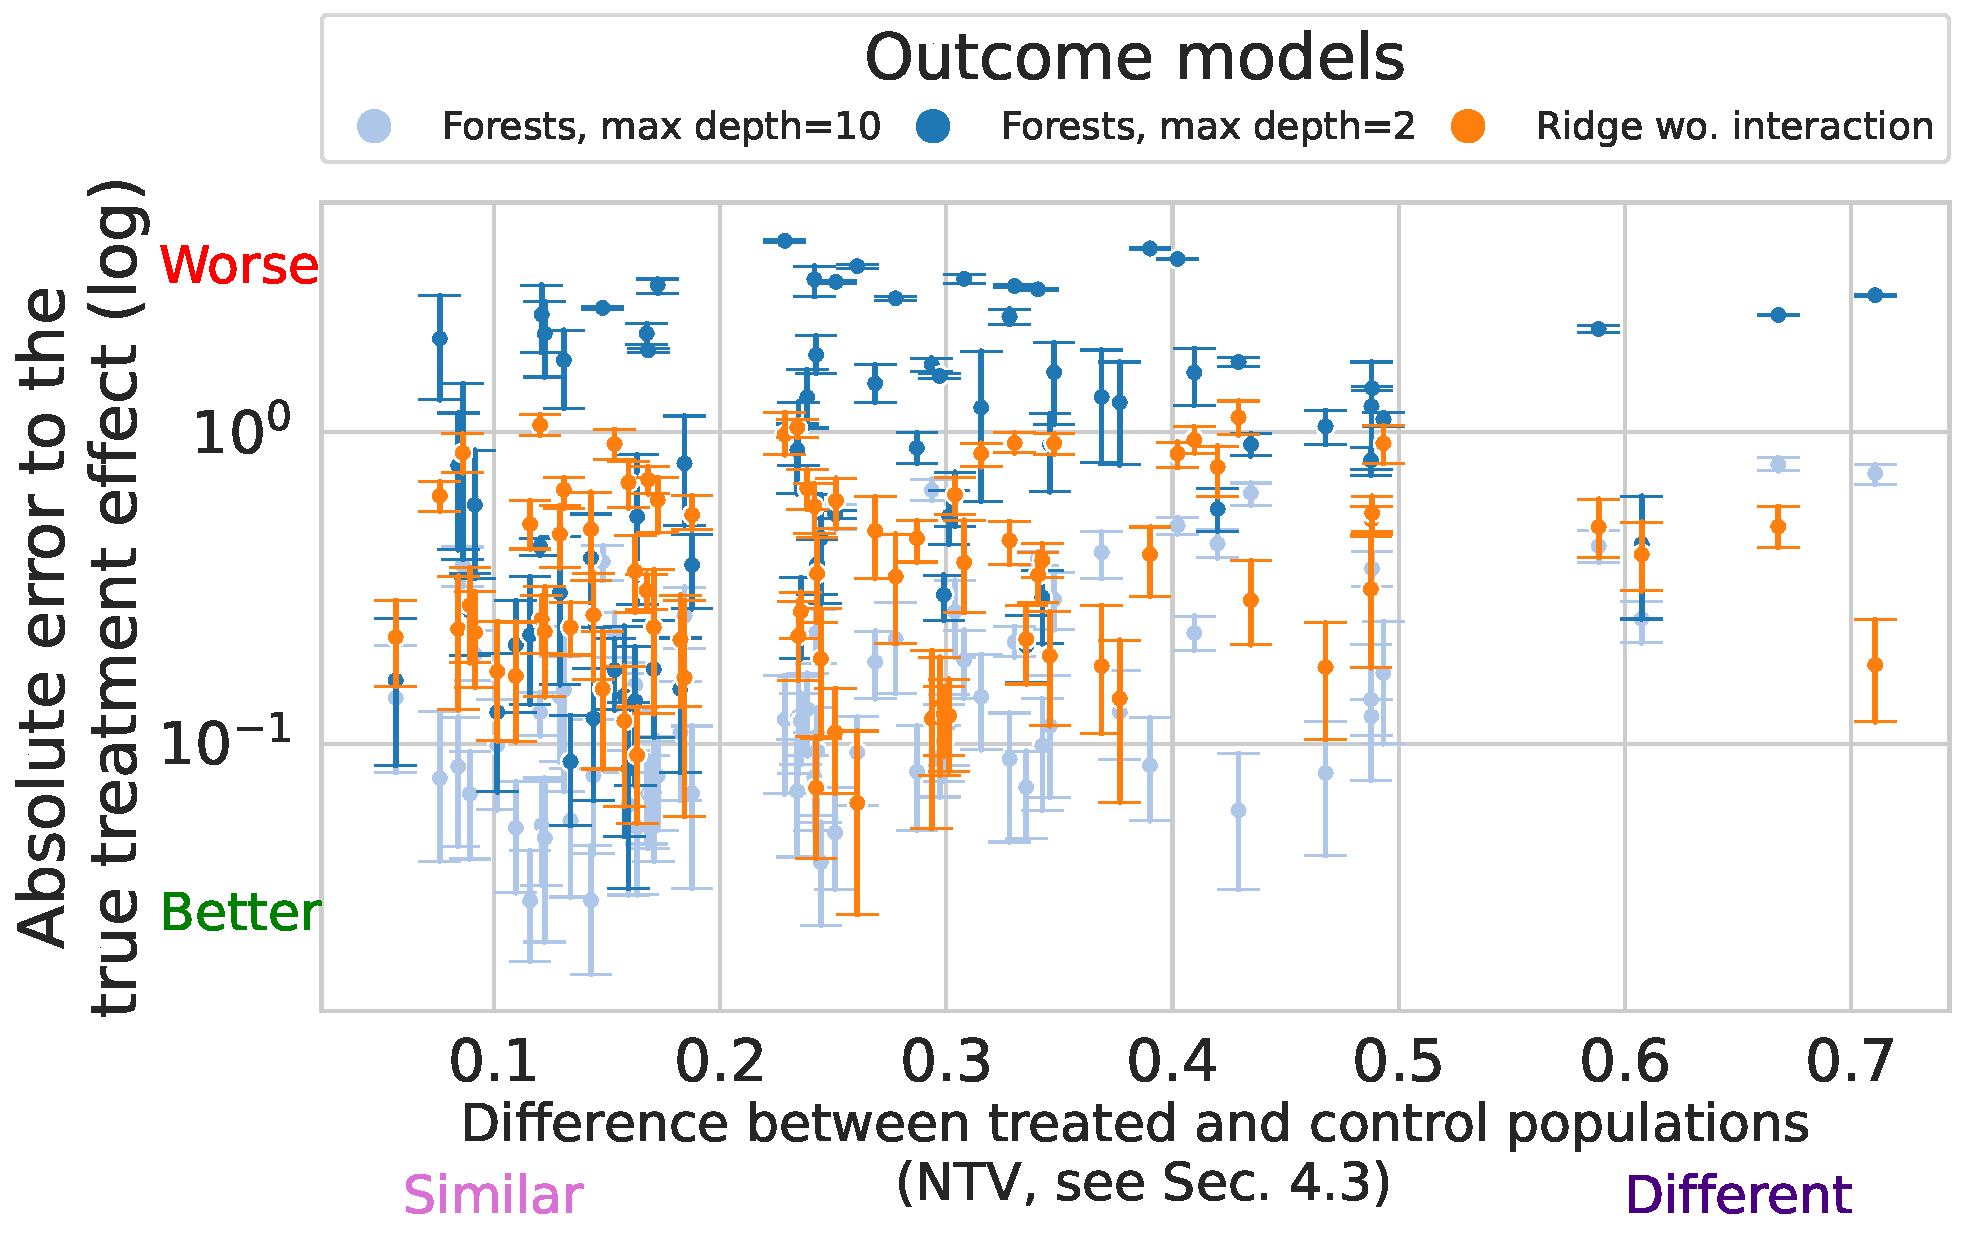
\includegraphics[width=0.95\linewidth]{2023-03-08-11-10-28_acic_2016_ate_heterogeneity.parquet_abs_bias_ylog_scale=True.pdf}%
        \caption{\textbf{Different outcome models lead to different
                estimation errors on the Average Treatment Effects},
            on 77 classic simulations with known true causal effect
            \cite{dorie_automated_2019}. The different models are ridge regression
            and random forests with different hyper-parameters
            (details
            \ref{apd:toy_example:acic_2016_ate_variability}). The different configurations are
            plotted as a function of increasing difference between treated and
            untreated population --see
            \autoref{subsec:measuring_overlap}.
            There is no systematic best performer; data-driven model
            selection is important.
            \label{fig:acic_2016_ate_heterogeneity}%
        }
    \end{figure}

    Outcome models are implemented with
    \href{https://scikit-learn.org/stable/}{scikit-learn}
    \cite{pedregosa_scikitlearn_2011} and the following hyper-parameters:

    \begin{table}[h!]
        \centering
        \begin{tabular}{llll}
            \toprule
            Outcome Model                                  & Hyper-parameters grid
            \\
            \midrule
            Random Forests                                 & Max depth: [2,
            10]                                                                    \\

            Ridge regression without treatment interaction & Ridge regularization:
            [0.1]                                                                  \\

            Ridge regression with treatment interaction    & Ridge regularization:
            [0.1]                                                                  \\
            \bottomrule
        \end{tabular}
        \caption{Hyper-parameters grid used for ACIC 2016 ATE variability}
        \label{apd:toy_example:acic_2016_ate_variability:table}
    \end{table}

    \section{Prior work : model selection for outcome modeling (g-computation)}\label{apd:prior_work}

    A natural way to select a predictive model for causal inference would be
    an error measure between a causal quantity such as the CATE and models' estimate. But such error is
    not a ``feasible'' risk: it cannot be computed solely from observed data
    and requires oracle knowledge.

    % XXX: I think that I should make the following paragraph shorter

    \paragraph{Simulation studies of causal model selection}

    Using eight simulations setups from \cite{powers_methods_2018}, where
    the oracle CATE is known, \cite{schuler_comparison_2018} compare four
    causal risks, concluding that for CATE estimation the best
    model-selection risk is the so-called $R\text{-risk}$
    \cite{nie_quasioracle_2017} --def.\,\ref{def:r_risk}, below. Their
    empirical results are clear for randomized treatment allocation but less
    convincing for observational settings where both simple Mean Squared
    Error --MSE, $\mu\text{-risk}(f)$ def.\,\ref{def:mu_risk}-- and
    reweighted MSE --$\mu\text{-risk}_{IPW}$ def.\,\ref{def:mu_ipw_risk}--
    appear to perform better than $R\text{-risk}$ on half of the simulations.
    Another work \cite{alaa_validating_2019} studied empirically both MSE and
    reweighted MSE risks on the semi-synthetic ACIC 2016 datasets
    \cite{dorie_automated_2019}, but did not include the $R\text{-risk}$. We complete these
    prior empirical work by studying a wider variety of data generative
    processes and varying the influence of overlap, an important parameter of
    the data generation process which makes a given causal metric appropriate
    \cite{damour_overlap_2020}. We also study how to best adapt
    cross-validation procedures to causal metrics which themselves come with
    models to estimate.

    \paragraph{Theoretical studies of causal model selection}

    Several theoretical works have proposed causal model selection procedures
    that are \emph{consistent}: select the best model in a family given
    asymptotically large data. These work rely on introducing a
    CATE estimator in the testing procedure: matching
    \cite{rolling_model_2014}, an IPW estimate
    \cite{gutierrez_causal_2016}, a doubly robust estimator
    \cite{saito_counterfactual_2020}, or debiasing the error with influence
    functions \cite{alaa_validating_2019}. However, for theoretical
    guarantees to hold, the test-set correction needs to converge to the
    oracle: it needs to be flexible enough --well-posed-- and asymptotic
    data. From a practical perspective, meeting such requirements
    implies having a good CATE estimate, thus having solved
    the original problem of causal model selection.

    \paragraph{Statistical guarantees on causal estimation procedures}

    Much work in causal inference has focused on procedures that
    guarantee asymptotically consistent estimators, such as Targeted
    Machine Learning
    Estimation (TMLE) \cite{laan_targeted_2011,schuler_targeted_2017} or
    Double Machine Learning \cite{chernozhukov_double_2018}. Here also, theories require asymptotic regimes and
    models to be \textit{well-specified}.

    By contrast, without assuming that estimators are well specified, there exists an upper bound
    on the oracle error to the CATE ($\tau\text{-risk}$) that involves the error on
    the outcome and the similarity of the distributions of treated and control
    patients \cite{johansson2022generalization}. However, they use this upper bound for model optimization,
    and do not give insights on model selection. In addition, for hyperparameter
    selection, they rely on a plugin estimate of the $\tau\text{-risk}$ built with
    counterfactual nearest neighbors, which has been shown ineffective
    \cite{schuler_comparison_2018}.


    \section{Causal assumptions}\label{apd:causal_assumptions}

    We assume the following four assumptions, referred as strong ignorability and
    necessary to assure identifiability of the causal estimands with observational
    data \cite{rubin_causal_2005}:
    \begin{assumption}[Unconfoundedness]\label{assumption:ignorability}
        \begin{equation*}\label{eq:ignorability}
            \{Y(0), Y(1) \} \indep A | X
        \end{equation*}
        This condition --also called ignorability-- is equivalent to the conditional
        independence on $e(X)$ \cite{rosenbaum_central_1983}: $\{Y(0), Y(1) \}
            \indep  A | e(X)$.
    \end{assumption}


    \begin{assumption}[Overlap, also known as Positivity)]\label{assumption:overlap}
        \begin{equation*}\label{eq:overlap}
            \eta < e(x) < 1 - \eta \quad \forall x \in \mathcal X \text{ and some } \eta > 0
        \end{equation*}
        The treatment is not perfectly predictable. Or with different words, every
        patient has a chance to be treated and not to be treated. For a given set of
        covariates, we need examples of both to recover the ATE.
    \end{assumption}

    As noted by \cite{damour_overlap_2020}, the choice of covariates $X$ can
    be viewed as a trade-off between these two central assumptions. A bigger
    covariates set generally reinforces the ignorability assumption. In the
    contrary, overlap can be weakened by large $\mathcal{X}$ because of the
    potential inclusion of instruments: variables only linked to the treatment which
    could lead to arbitrarily small propensity scores.

    % remark: There is a major counter example to these colliders (variables which
    % are caused by both the outcome and the treatment),

    \begin{assumption}[Consistency]\label{assumption:consistency} The observed
        outcome is the potential outcome of the assigned treatment:
        \begin{equation*}\label{eq:consistancy}
            Y = A \, Y(1) + (1-A) \, Y(0)
        \end{equation*}
        Here, we assume that the intervention $A$ has been well defined. This
        assumption focuses on the design of the experiment. It clearly states the link
        between the observed outcome and the potential outcomes through the
        intervention \cite{hernan_causal_2020}.
    \end{assumption}

    \begin{assumption}[Generalization]\label{assumption:generalization} The training
        data on which we build the estimator and the test data on which we make the
        estimation are drawn from the same distribution $\mathcal D^*$, also known as
        the ``no covariate shift'' assumption \cite{jesson_identifying_2020}.
    \end{assumption}

    \section{Definitions of feasible risks}\label{def:feasible_risks}


    \begin{definition}[Factual $\mu\text{-risk}$]\label{def:mu_risk}
        \cite{shalit_estimating_2017} This is the usual Mean Squared Error on
        the target y. It is what is typically meant by ``generalization error'' in
        supervised learning:
        \begin{equation*}\label{eq:mu_risk}
            \mu\text{-risk}(f)=\mathbb{E}\left[(Y-f(X ; A))^2 \right]
        \end{equation*}
    \end{definition}


    \begin{definition}[$\mu\text{-risk}_{IPW}^{\star}$]\label{def:mu_ipw_risk}
        \cite{vanderlaan_unified_2003} Let the inverse propensity weighting
        function $w(x, a) = \frac{a}{e(x)} + \frac{1 - a}{1 - e(x)}$, we define the
        semi-oracle Inverse Propensity Weighting risk,
        \begin{equation*}\label{eq:mu_ipw_risk}
            \mu\text{-risk}_{IPW}^{\star}(f) = \mathbb{E}\left[ \Big( \frac{A}{e(X)} + \frac{1-A}{1-e(X)} \Big) (Y-f(X ; A))^2 \right]
        \end{equation*}
    \end{definition}

    \smallskip


    \begin{definition}[$\tau\text{-risk}^{\star}_{IPW}$]\label{def:tau_ipw_risk}
        \cite{wager_estimation_2018}
        The CATE $\tau(x)$ can be estimated with a
        regression against inverse propensity weighted outcomes \cite{
            athey2016recursive,gutierrez_causal_2016,wager_estimation_2018},
        the $\tau\text{-risk}_{IPW}$.
        \begin{equation*}
            \tau\text{-risk}^{\star}_{IPW}(f) =\mathbb{E}
            \left[ \Big(Y \frac{A - e(X)}{e(X)
                    (1-e(X))}-\tau_f\left(X\right)\Big)^2 \right]
            %  =\mathbb{E}_{(Y, X, A)
            %            \sim \mathcal D} \left[ \left(Y \left( \frac{A}{e(X)} -
            %            \frac{1-A}{1-e(X)}\right)-\tau_f\left(X\right)\right)^2 \right]
        \end{equation*}
    \end{definition}

    \begin{definition}[$U\text{-risk}^{\star}$]\label{def:u_risk}
        \cite{kunzel_metalearners_2019,nie_quasioracle_2017} Based on
        the Robinson decomposition --eq. \ref{eq:r_decomposition}, the U-learner
        uses the $A-e(X)$ term
        in the denominator. The derived risk is:
        \begin{equation*}
            U\text{-risk}^{\star}(f) =\mathbb{E}
            \left[
                \left( \frac{Y-m\left(X\right)}{A-e\left(X\right)} -
                \tau_f\left(X\right)\right)^{2} \right]
        \end{equation*}
        Note that extreme propensity weights in the
        denominator term might inflate errors in the numerator due to imperfect
        estimation of the mean outcome $m$.
    \end{definition}

    \begin{definition}[$R\text{-risk}^{\star}$]\label{def:r_risk}
        \cite{nie_quasioracle_2017,schuler_comparison_2018}
        The $R\text{-risk}$ also uses two nuisance $m$ and $e$:
        \begin{equation*}
            R\text{-risk}^{\star}(f) =\mathbb{E} \big[
                \big(\left(Y-m\left(X\right)\right) -\left(A-e\left(X\right)\right) \tau_f\left(X\right)\big)^{2} \big]
        \end{equation*}
    \end{definition}

    It is also based on the Robinson decomposition --eq. \ref{eq:r_decomposition}. %It performs well in various
    %simulations, estimating the nuisances
    %$(\check e, \check m)$ with
    %lasso, boosting or kernel ridge regressions
    %\cite{nie_quasioracle_2017}.

    \section{Proofs: Links between feasible and oracle risks}\label{apd:proofs}

    % \subsection{Upper bound of $\tau\text{-risk}$ with
    %     $\mu\text{-risk}_{IPW}$}\label{apd:proofs:mu_risk_ipw_bound}

    % For the bound with the $\mu\text{-risk}_{IPW}$, we will decompose the CATE risk
    % on each factual population risks:

    % \begin{definition}[Population Factual $\mu\text{-risk}$]\label{mu_risk_a}
    %     \cite{shalit_estimating_2017}
    %     \begin{equation*}
    %         \mu\text{-risk}_{a}(f)= \int_{\mathcal Y \times \mathcal X} (y-f(x ; A=a))^{2}  p(y ; x=x \mid A=a) \; dy dx
    %     \end{equation*}
    % \end{definition}

    % Applying Bayes rule, we can decompose the $\mu\text{-risk}$ on each
    % intervention:
    % \begin{equation*}
    %     \mu\text{-risk}(f)
    %     =p_{A} \,\mu\text{-risk}_{1}(f)+\left(1-p_{A}\right) \,\mu\text{-risk}_{0}(f)
    %     \text{with } p_A=\mathbb P(A=1)
    % \end{equation*}

    % These definitions allows to state a intermediary result on each population:
    % \begin{lemma}[Mean-variance decomposition]\label{apd:proofs:mu_risk_ipw_link_mu}
    %     We need a reweighted version of the classical mean-variance decomposition.

    %     For an outcome model $f: x \times A \rightarrow \mathcal X$. Let the inverse
    %     propensity weighting function $w(a ; x)=a e(x)^{-1}+(1-a)(1-e(x))^{-1}$.
    %     \begin{align*}
    %          & \int_{\mathcal X}(\mu_{1}(x)-f(x ; 1))^{2} p(x) dx  = p_{A} \mu\text{-risk}_{IPW, 1}(w, f)  -\sigma^{2}_{Bayes}(1)
    %     \end{align*}
    %     And
    %     \begin{align*}
    %          & \int_{\mathcal X}(\mu_{0}(x)-f(x; 0))^{2} p(x) dx   = (1-p_A) \mu\text{-risk}_{IPW, 0}(w, f)  -\sigma^{2}_{Bayes}(0)
    %     \end{align*}

    %     \begin{proof}
    %         \begin{align*}
    %              & p_{A} \mu\text{-risk}_{IPW, 1}(w, f)  = \int_{\mathcal X \times \mathcal Y} \frac{1}{e(x)}(y-f(x ; 1))^{2} p(y \mid x ; A=1) p(x ; A=1) d y d x                                                      \\
    %              & = \int_{\mathcal X \times \mathcal Y} (y-f(x ; 1))^{2} p(y \mid x ; A=1) \frac{p(x ; A=1)}{p(x ; A=1)}p(x)dy dx                                                                                      \\
    %              & = \int_{\mathcal X \times \mathcal Y} \big[(y-\mu_1(x))^{2}+\left(\mu_{1}(x)-f(x ; 1)\right)^{2} + 2\left(y-\mu_{1}(x)\right)\left(\mu_{1}(x)-f(x, 1)\right) \big] p(y \mid x ; A=1) p(x) d y d x    \\
    %              & =\int_{\mathcal X} \big [ \int_{\mathcal Y} (y-\mu_1(x))^{2} p(y \mid x ; A=1) dy\big ] p(x)dx + \int_{\mathcal X \times \mathcal Y} \left(\mu_{1}(x)-f(x ; 1)\right)^{2} p(x)p(y \mid x ; A=1)dx dy \\
    %              & + \qquad 2 \int_{\mathcal X} \big [ \int_{\mathcal Y} \left(y-\mu_{1}(x)\right) p(y \mid x ; A=1) dy \big ] \left(\mu_{1}(x)-f(x, 1)\right)p(x)dx                                                    \\
    %              & =\int_{\mathcal X} \sigma_{y}^{2}(x, 1) p(x) d x +\int_{\mathcal X} \left(\mu_{1}(x)-f(x ; 1)\right)^{2} p(x) d x+0
    %         \end{align*}
    %     \end{proof}
    % \end{lemma}

    % \begin{proposition*}[Upper bound with mu-IPW]\label{apd:proofs:prop:upper_bound}
    %     Let f be a given outcome model, let the weighting function $w$ be the Inverse
    %     Propensity Weight $w(x; a) = \frac{a}{e(x)} + \frac{1-a}{1-e(x)}$. Then, under
    %     overlap (assumption \ref{assumption:overlap}),
    %     \begin{align*}
    %         \tau\text{-risk}(f) \leq & \; 2 \, \mu\text{-risk}_{IPW}(w, f)  \; - 2 \, (\sigma^2_{Bayes}(1) +  \sigma^2_{Bayes}(0))
    %     \end{align*}

    %     \begin{proof}
    %         \begin{align*}
    %              & \tau\text{-risk}(f) =\int_{\mathcal X}(\mu_{1}(x)-\mu_{0}(x)-(f(x ; 1)-f(x ; 0))^{2} p(x) d x
    %         \end{align*}
    %         By the triangle inequality $(u+v)^2 \leq 2(u^2 + v^2)$:
    %         \begin{align*}
    %              & \tau\text{-risk}(f) \leq
    %             2 \int_{\mathcal X}\big[\left(\mu_{1}(x)-f(x ; 1)\right)^{2}+\left(\mu_{0}(x)-f(x ; 0)\right)^{2}\big] p(x) d x \\
    %         \end{align*}
    %         Applying Lemma \ref{apd:proofs:mu_risk_ipw_link_mu},
    %         \begin{align*}
    %              & \tau\text{-risk}(f) \leq 2\big[p_A \mu\text{-risk}_{IPW, 1}(w, f) +(1-p_A) \mu\text{-risk}_{IPW, 0}(w, f)(w, f)\big] -2(\sigma^{2}_{Bayes}(0) + \sigma^{2}_{Bayes}(1)) \\
    %              & = 2 \mu\text{-risk}_{IPW}(w, f)-2(\sigma^{2}_{Bayes}(0) + \sigma^{2}_{Bayes}(1))
    %         \end{align*}
    %     \end{proof}
    % \end{proposition*}



    \subsection{Reformulation of the $R\text{-risk}$ as reweighted
        $\tau\text{-risk}$}\label{apd:proofs:r_risk_rewrite}

    \begin{proposition*}[$R\text{-risk}$ as reweighted $\tau
                \text{-risk}$]\label{apd:proofs:prop:r_risk_rewrite}

        \begin{proof}

            We consider the R-decomposition: \cite{robinson_rootnconsistent_1988},
            \begin{equation}\label{apd:eq:r_decomposition}
                y(a) = m(x) + \big( a - e(x) \big) \tau(x) + \varepsilon(x; a)
            \end{equation}
            Where $\mathbb E[\varepsilon(X; A)|X, A] = 0$ We can use it as plug in the
            $R\text{-risk}$ formula:

            \begin{align*}
                 & R\text {-risk}(f) =\int_{\mathcal{Y} \times \mathcal{X} \times \mathcal{A}}[(y-m(x))-\big(a-e(x)\big) \tau_f(x)]^{2} p(y ; x ; a) d y d x d a                                     \\
                 & =\int_{\mathcal{Y} \times \mathcal{X} \times \mathcal{A}} \left[\big(a-e(x)\big)\tau(x)+\varepsilon(x ; a)-\big(a-e(x)\big) \tau_f(x)\right]^{2} p(y ; x ; a) d y d x da          \\
                 & =\int_{\mathcal{X} \times \mathcal{A}}\big(a-e(x)\big)^{2}\big(\tau(x)- \tau_f(x)\big)^{2} p(x ; a) d x d a                                                                       \\
                 & + 2  \int_{\mathcal{Y} \times \mathcal{X} \times \mathcal{A}}\big(a-e(x)\big)\big(\tau(x)-\tau_f(x)\big)  \int_{\mathcal{Y}} \varepsilon(x ; a) p(y \mid x ; a) d y p(x ; a)dx da \\
                 & +\int_{\mathcal{X} \times \mathcal{A}} \int_{\mathcal{Y}} \varepsilon^{2}(x ; a) p(y \mid x ; a) d y p(x ; a) d x d a
            \end{align*}

            The first term can be decomposed on control and treated populations to force
            $e(x)$ to appear:
            \begin{align*}
                 & \int_{\mathcal{X}}\big(\tau(x)-\tau_f(x)\big)^{2}\left[e(x)^{2}p(x;0) + \big(1-e(x)\big)^{2} p(x;1)\right] d x                    \\
                 & =\int_{\mathcal{X}}\big(\tau(x)-\tau_f(x)\big)^{2}  \left[e(x)^{2}\big(1-e(x)\big)p(x) + \big(1-e(x)\big)^{2}e(x) p(x)\right] d x \\
                 & =\int_{\mathcal{X}}(\tau(x)-\tau_f(x))^{2}(1-e(x)) e(x)[1-e(x)+e(x)] p(x) d x                                                     \\ &=\int_{\mathcal{X}}(\tau(x)-\tau_f(x))^{2}(1-e(x)) e(x) p(x) d x.
            \end{align*}

            The second term is null since, $\mathbb E[\varepsilon(x, a) |X, A]=0$.

            The third term corresponds to the modulated residuals \ref{eq:residuals} :
            $\tilde{\sigma}_B^2(0) + \tilde{\sigma}_B^2(1)$

        \end{proof}
    \end{proposition*}

    \subsection{Interesting special cases}\label{apd:theory:special_cases}

    \paragraph{Randomization special case}\label{remark:rct} If the treatment is
    randomized as in RCTs, $p(A=1 \mid X=x) = p(A=1)=p_A$, thus
    $\mu\text{-risk}_{IPW}$ takes a simpler form:
    \begin{equation*}
        \mu\text{-risk}_{IPW} = \mathbb{E}_{(Y, X, A) \sim \mathcal D}\left[ \Big( \frac{A}{p_A} + \frac{1-A}{1-p_A} \Big) (Y-f(X ; A))^2 \right]
    \end{equation*}
    However, we still can have large differences
    between $\tau\text{-risk}$ and $\mu\text{-risk}_{IPW}$ coming from heterogeneous
    errors between populations as shown experimentally in \cite{schuler_comparison_2018} and our
    results below.

    Concerning the $R\text{-risk}$, replacing $e(x)$ by its randomized value $p_A$
    in Proposition \ref{theory:prop:r_risk_rewrite} yields the oracle
    $\tau\text{-risk}$ up to multiplicative and additive constants:
    \begin{equation*}
        R\text{-risk} = p_A \, (1-p_A) \, \tau\text{-risk} \;+\; (1 - p_A) \,\sigma_B^2(0) \;+\; p_A \sigma_B^2(1)
    \end{equation*}
    Thus, selecting estimators with $R\text{-risk}^*$ in
    randomized setting controls the $\tau\text{-risk}$. This explains
    the strong performances of $R\text{-risk}$ in randomized setups
    \cite{schuler_comparison_2018} and is a strong argument to use it
    to estimate heterogeneity in RCTs.

    \paragraph{Oracle Bayes predictor}\label{remark:bayes_oracle} If we
    have access to the oracle Bayes predictor for the outcome ie.~$f(x,
        a)=\mu(x, a)$, then all risks are equivalent up to the residual variance:
    \begin{equation}
        \tau\text{-risk}(\mu) = \mathbb E_{X\sim p(X)}[(\tau(X) - \tau_{\mu}(X))^2] = 0
    \end{equation}
    \begin{align}
        \mu\text{-risk}(\mu) & = \mathbb E_{(Y, X, A) \sim p(Y;X;A)}[\big( Y - \mu_A(X)\big)^2] \\
                             & = \int_{\mathcal X, \mathcal A}
        \,\varepsilon(x,a)^2 p(a \mid x) \,p(x) \,dx\,da  \leq \sigma_B^{2}(0) + \sigma_B^{2}(1) \nonumber
    \end{align}
    \begin{equation}
        \mu\text{-risk}_{IPW}(\mu) = \sigma_B^{2}(0) + \sigma_B^{2}(1)  \quad \text{from Lemma \ref{apd:proofs:mu_risk_ipw_link_mu}}
        %\notag
    \end{equation}
    \begin{multline}
        R\text{-risk}(\mu) = \tilde{\sigma}_B^{2}(0) + \tilde{\sigma}_B^{2}(1)
        \leq \sigma_B^{2}(0) + \sigma_B^{2}(1)  \\  \text{from Proposition \ref{theory:prop:r_risk_rewrite}}%\notag
    \end{multline}

    Thus, differences between causal risks only matter in finite sample regimes.
    Universally consistent learners converge to the Bayes risk in asymptotic
    regimes, making all model selection risks equivalent. In practice however,
    choices must be made in non-asymptotic regimes.


    \section{Measuring overlap}\label{apd:motivation_ntv}

    \paragraph{Motivation of the Normalized Total Variation}

    %\idea{A simplier measure, NTV seems to capture what we want}

    Overlap is often assessed by comparing visually population distributions as in
    Figure \ref{fig:toy_example} or computing standardized difference on each
    feature \cite{austin_introduction_2011,austin_moving_2015}. While these methods
    are useful to decide if positivity holds, they do not yield a single measure.
    Rather, we compute the divergence between the population covariate distributions
    $\mathbb P(X|A=0)$ and $\mathbb P(X|A=1)$
    \cite{damour_overlap_2020,johansson2022generalization}. Computing overlap when
    working only on samples of the observed distribution, outside of simulation,
    requires a sophisticated estimator of discrepancy between distributions, as two
    data points never have the same exact set of features. Maximum Mean Discrepancy
    \cite{gretton2012kernel} is typically used in the context of causal inference
    \cite{shalit_estimating_2017,johansson2022generalization}. However it needs a
    kernel, typically Gaussian, to extrapolate across neighboring observations. We
    prefer avoiding the need to specify such a kernel, as it must be adapted to the
    data which is tricky with categorical or non-Gaussian features, a common
    situation for medical data.

    For simulated and some semi-simulated data, we have access to the probability of
    treatment for each data point, which sample both densities in the same data
    point. Thus, we can directly use distribution discrepancy measures and rely on
    the Normalized Total Variation (NTV) distance to measure the overlap between the
    treated and control propensities. This is the empirical measure of the total
    variation distance \cite{sriperumbudur_integral_2009} between the distributions,
    $TV(\mathbb{P}(X|A=1), \mathbb{P}(X|A=0))$. As we have both distribution sampled
    on the same points, we can rewrite it a sole function of the propensity score, a
    low dimensional score more tractable than the full distribution $\mathbb
        P(X|A)$:

    \begin{equation}\label{eq:ntv}
        \widehat{NTV}(e, 1-e) = \frac{1}{2N} \sum_{i =1}^{N} \big |\frac{e(x_i)}{p_A}-\frac{1-e(x_i)}{1-{p_A}} \big |
    \end{equation}

    Formally, we can rewrite NTV as the Total Variation distance
    between the two population distributions. For a population $O = (Y(A), X, A)
        \sim \mathcal{D}$:

    \begin{align*}
        NTV(O) & = \frac{1}{2N} \sum_{i =1}^{N} \big | \frac{e(x_i)}{p_A}-\frac{1-e(x_i)}{1-{p_A}} \big|         \\
               & = \frac{1}{2N} \sum_{i =1}^{N} \big|\frac{P(A=1|X=x_i)}{p_A}-\frac{P(A=0|X=x_i)}{1-{p_A}} \big|
    \end{align*}

    Thus NTV approximates the following quantity in expectation over the data
    distribution $\mathcal{D}$:

    \begin{align*}
        NTV(\mathcal{D}) & = \int_{\mathcal{X}} \big | \frac{p(A=1|X=x)}{p_A}-\frac{p(A=0|X=x)}{1-{p_A}} \big | p(x)dx \\
                         & = \int_{\mathcal{X}} \big | \frac{p(A=1, X=x)}{p_A}-\frac{p(A=0, X=x)}{1-{p_A}} \big |dx    \\
                         & = \int_{\mathcal{X}} \big | p(X=x|A=1)- p(X=x|A=0) \big |dx
    \end{align*}

    For countable sets, this expression corresponds to the Total Variation distance
    between treated and control populations covariate distributions : $TV(p_0(x),
        p_1(x))$.

    \paragraph{Measuring overlap without the oracle propensity scores:} For ACIC
    2018, or for non-simulated data, the true propensity scores are not known. To
    measure overlap, we rely on flexible estimations of the Normalized Total
    Variation, using gradient boosting trees to approximate the propensity score.
    Empirical arguments for this plug-in approach is given in Figure
    \ref{apd:overlap:ntv_approximation}.

    \paragraph{Empirical arguments}

    We show empirically that NTV is an appropriate measure of overlap by :
    \begin{itemize}
        \item Comparing the NTV distance with the MMD for Caussim which is gaussian
              distributed in Figure \ref{apd:overlap:caussim:mmd_vs_ntv},
        \item Verifying that setups with penalized overlap from ACIC 2016 have a
              higher total variation distance than unpenalized setups in Figure
              \ref{apd:overlap:penalized_overlap}.
        \item Verifying that the Inverse Propensity Weights extrema (the inverse of
              the $\nu$ overlap constant appearing in the overlap Assumption
              \ref{assumption:overlap}) positevely correlates with NTV for Caussim,
              ACIC 2016 and Twins in Figure \ref{apd:ntv_vs_max_ipw}. Even if the same
              value of the maximum IPW could lead to different values of NTV, we
              expect both measures to be correlated : the higher the extrem propensity
              weights, the higher the NTV.
    \end{itemize}


    \paragraph{Estimating NTV in practice}

    Finally, we verify that approximating the NTV distance with a learned plug-in
    estimates of e(x) is reasonnable. We used either a logistic regression or a
    gradient boosting classifier to learn the propensity models for the three
    datasets where we have access to the ground truth propensity scores: Caussim,
    Twins and ACIC 2016. We respectively sampled 1000, 1000 and 770 instances of
    these datasets with different seeds and overlap settings. We first run a
    hyperparameter search with cross-validation on the train set, then select the
    best estimator. We refit on the train set this estimator with or without
    calibration by cross validation and finally estimate the normalized TV with the
    obtained model. This training procedure reflects the one described in Algorithm
    \ref{problem:estimation_procedure:algo} where nuisance models are fitted only on
    the train set.

    The hyper parameters are : learning rate $ \in [1e-3, 1e-2, 1e-1, 1]$, minimum
    samples leaf $\in [2, 10, 50, 100, 200]$ for boosting and L2 regularization $\in
        [1e-3, 1e-2, 1e-1, 1]$ for logistic regression.

    Results in Figure \ref{apd:overlap:ntv_approximation} comparing bias to the true
    normalized Total Variation of each dataset instances versus growing true NTV
    indicate that calibration of the propensity model is crucial to recover a good
    approximation of the NTV.




    \begin{figure}
        \begin{subfigure}[b]{\textwidth}
            \centering
            \caption{\textbf{Uncalibrated classifiers}}
            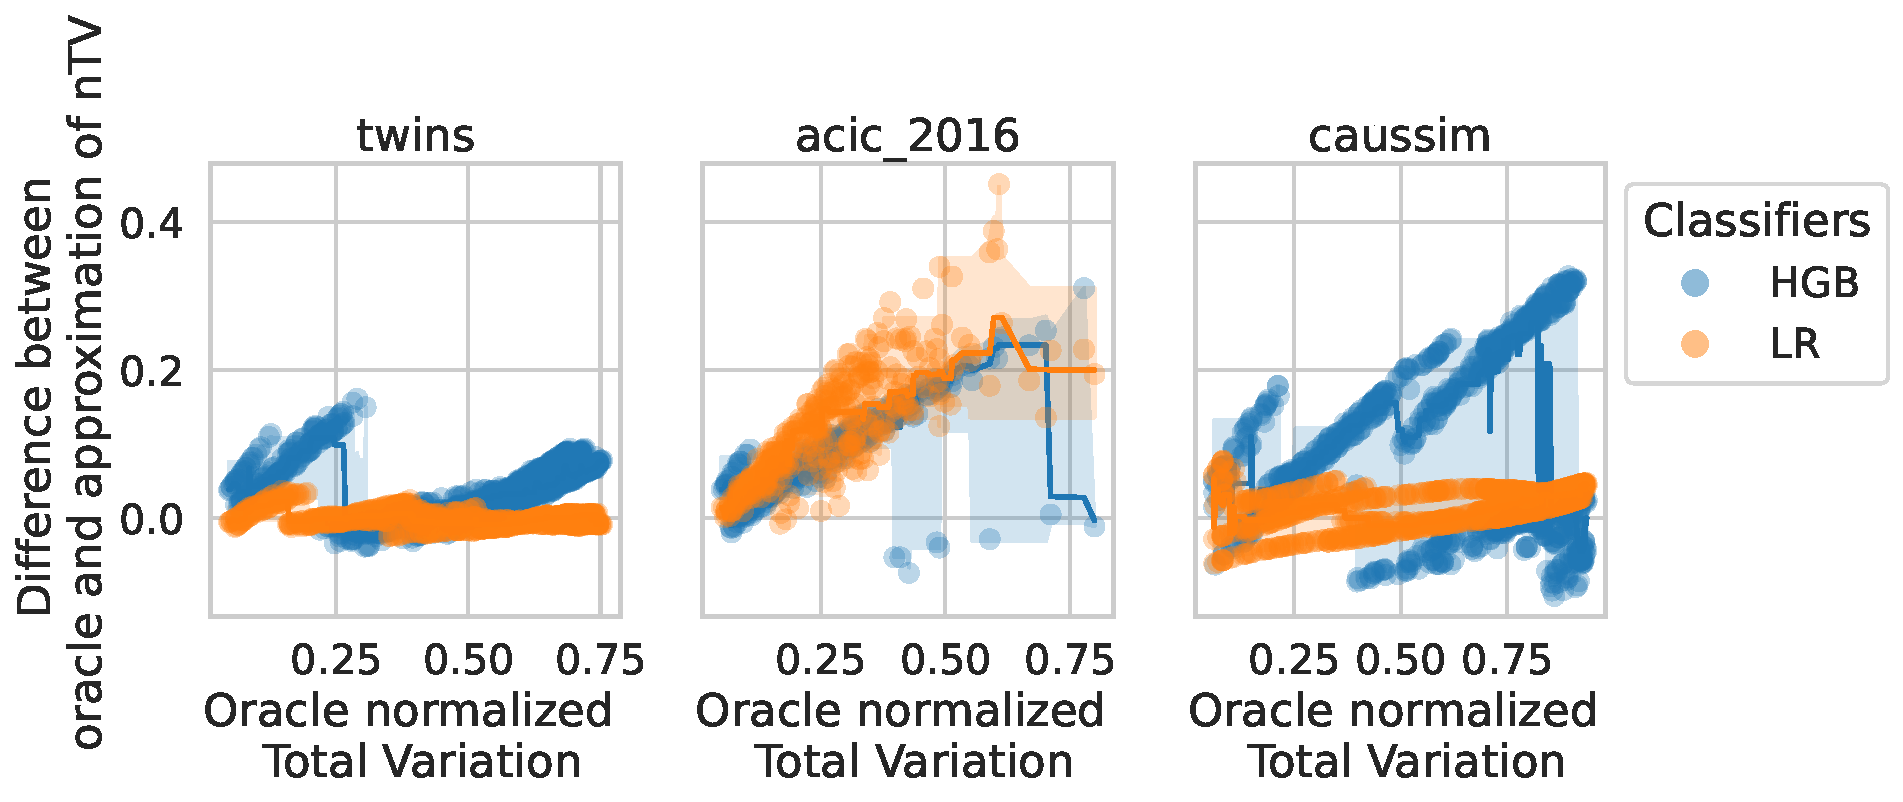
\includegraphics[width=\linewidth]{overlap_measure_diff_oracle_ntv_to_n_tv_calibration=False_vs_oracle_n_tv.pdf}
        \end{subfigure}
        \begin{subfigure}[b]{\textwidth}
            \centering
            \caption{\textbf{Calibrated
                    classifiers}}
            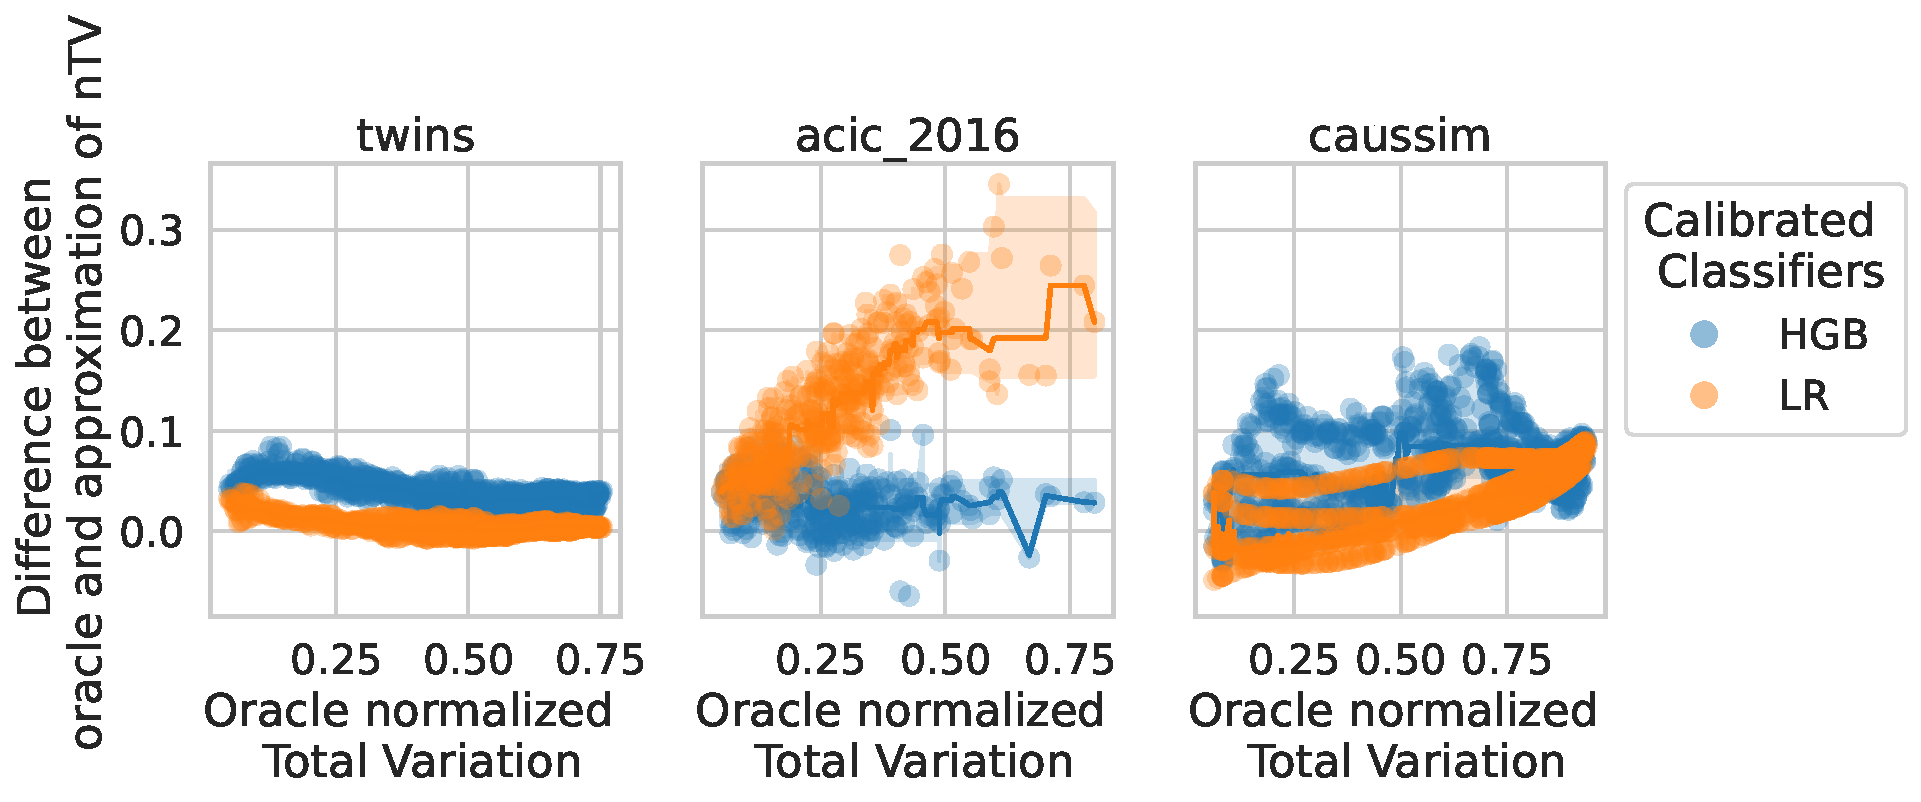
\includegraphics[width=\linewidth]{overlap_measure_diff_oracle_ntv_to_n_tv_calibration=True_vs_oracle_n_tv.pdf}
        \end{subfigure}
        \caption{a) Without calibration, estimation of NTV is not trivial even for
            boosting models. b) Calibrated classifiers are able to recover the true
            Normalized Total Variation for all datasets where it is
            available.}\label{apd:overlap:ntv_approximation}
    \end{figure}



    \begin{figure}
        \centering
        \caption{NTV recovers well the overlap settings described in the ACIC paper
            \cite{dorie_automated_2019}}\label{apd:overlap:penalized_overlap}
        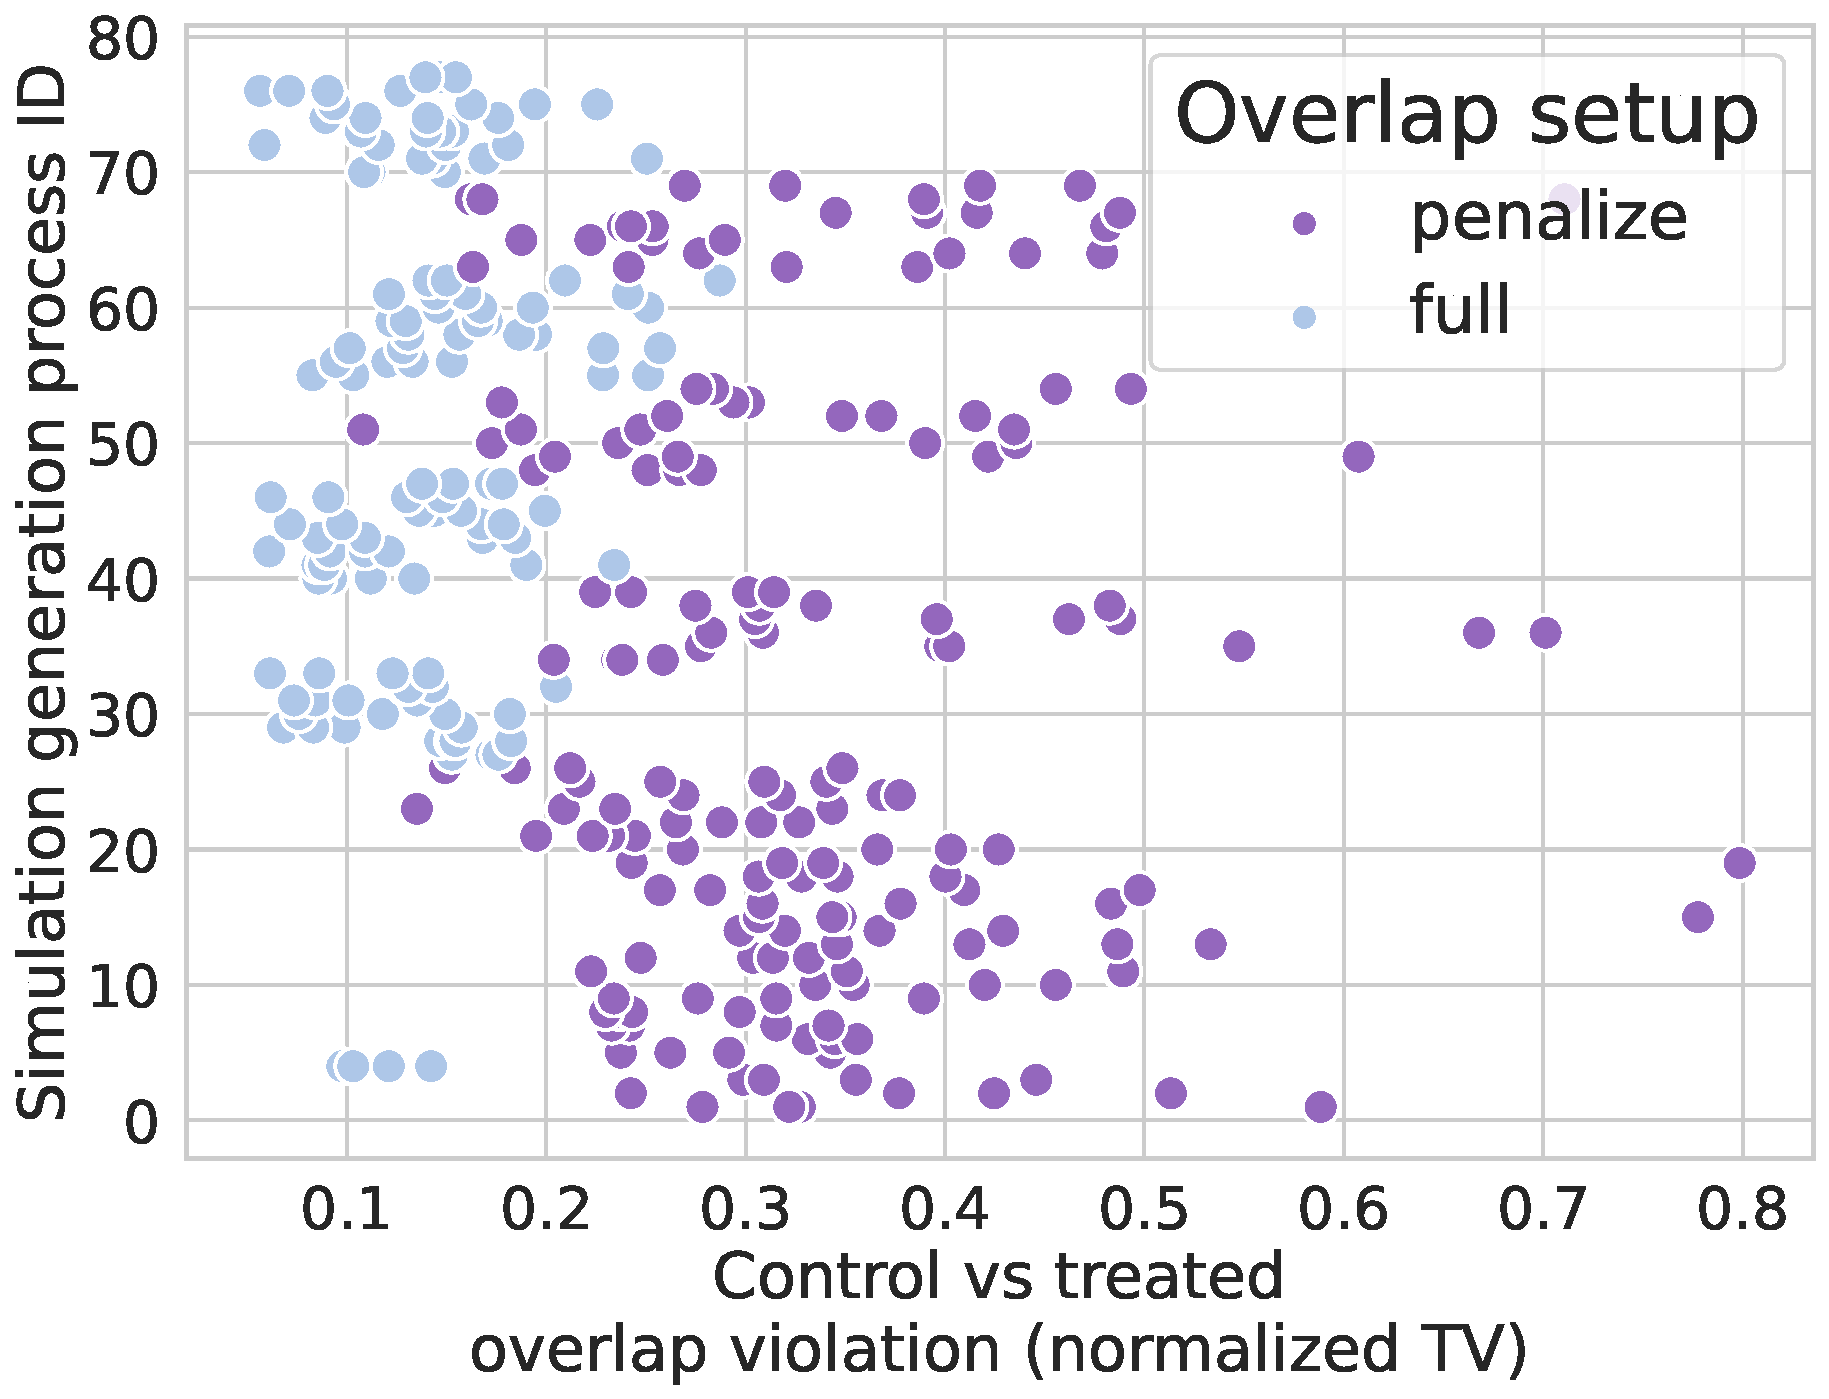
\includegraphics[width=0.7\linewidth]{overlap_measure_acic_2016_recovery_overlap_setup.pdf}
    \end{figure}


    \begin{figure}[htbp]
        \centering
        \caption{Good correlation between overlap measured as normalized Total
            Variation and Maximum Mean Discrepancy (200 sampled Caussim
            datasets)}\label{apd:overlap:caussim:mmd_vs_ntv}
        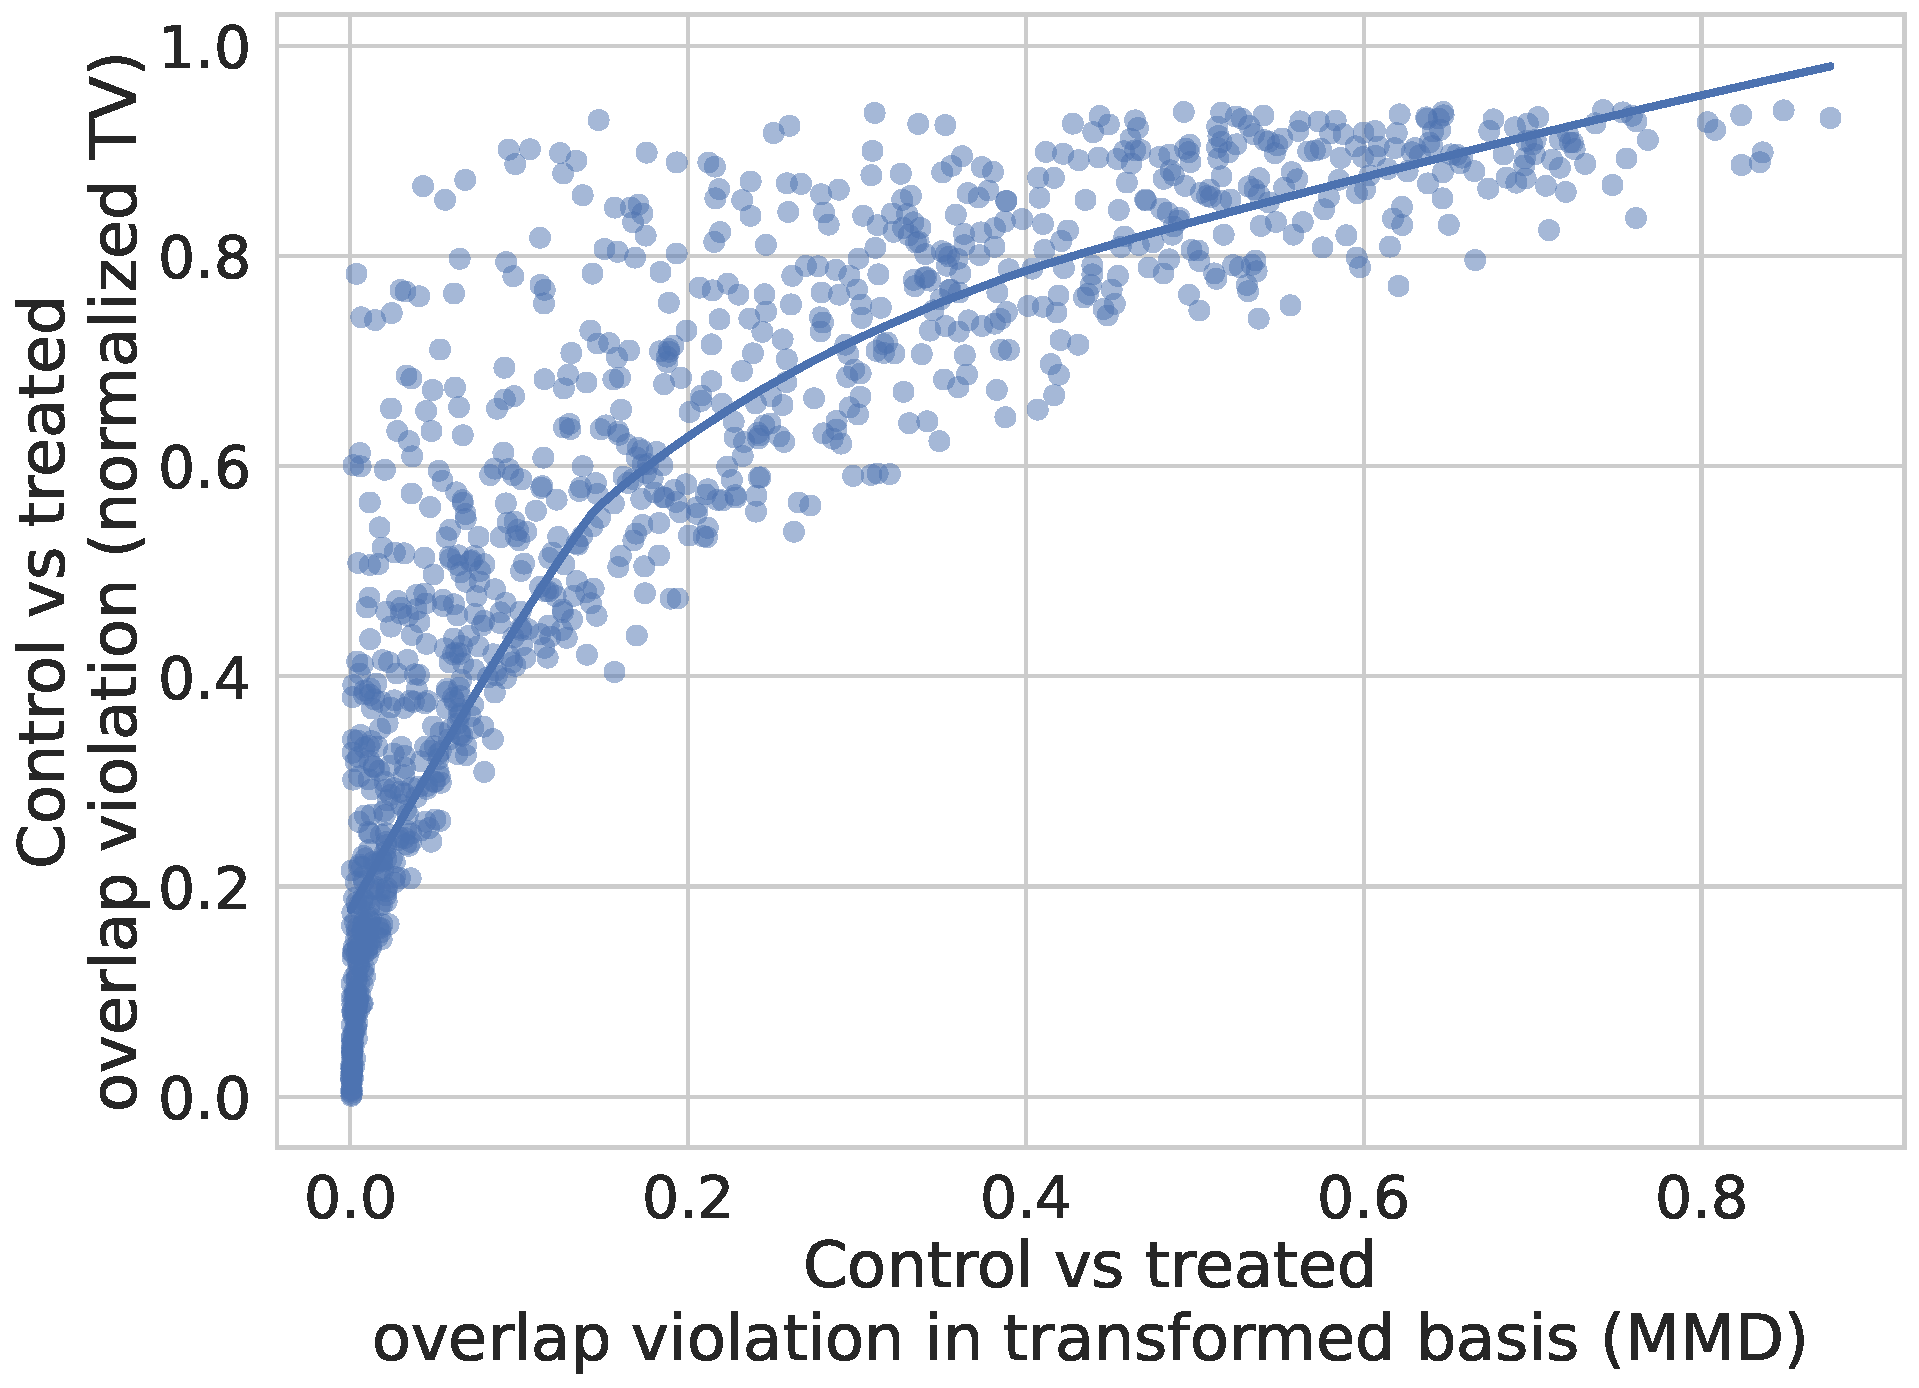
\includegraphics[width=0.7\linewidth]{overlap_measure_caussim_transformed_mmd_vs_ntv.pdf}
    \end{figure}


    \begin{figure}[ht]
        \centering
        \begin{subfigure}[b]{0.47\textwidth}
            \centering
            \caption{\textbf{Caussim}}
            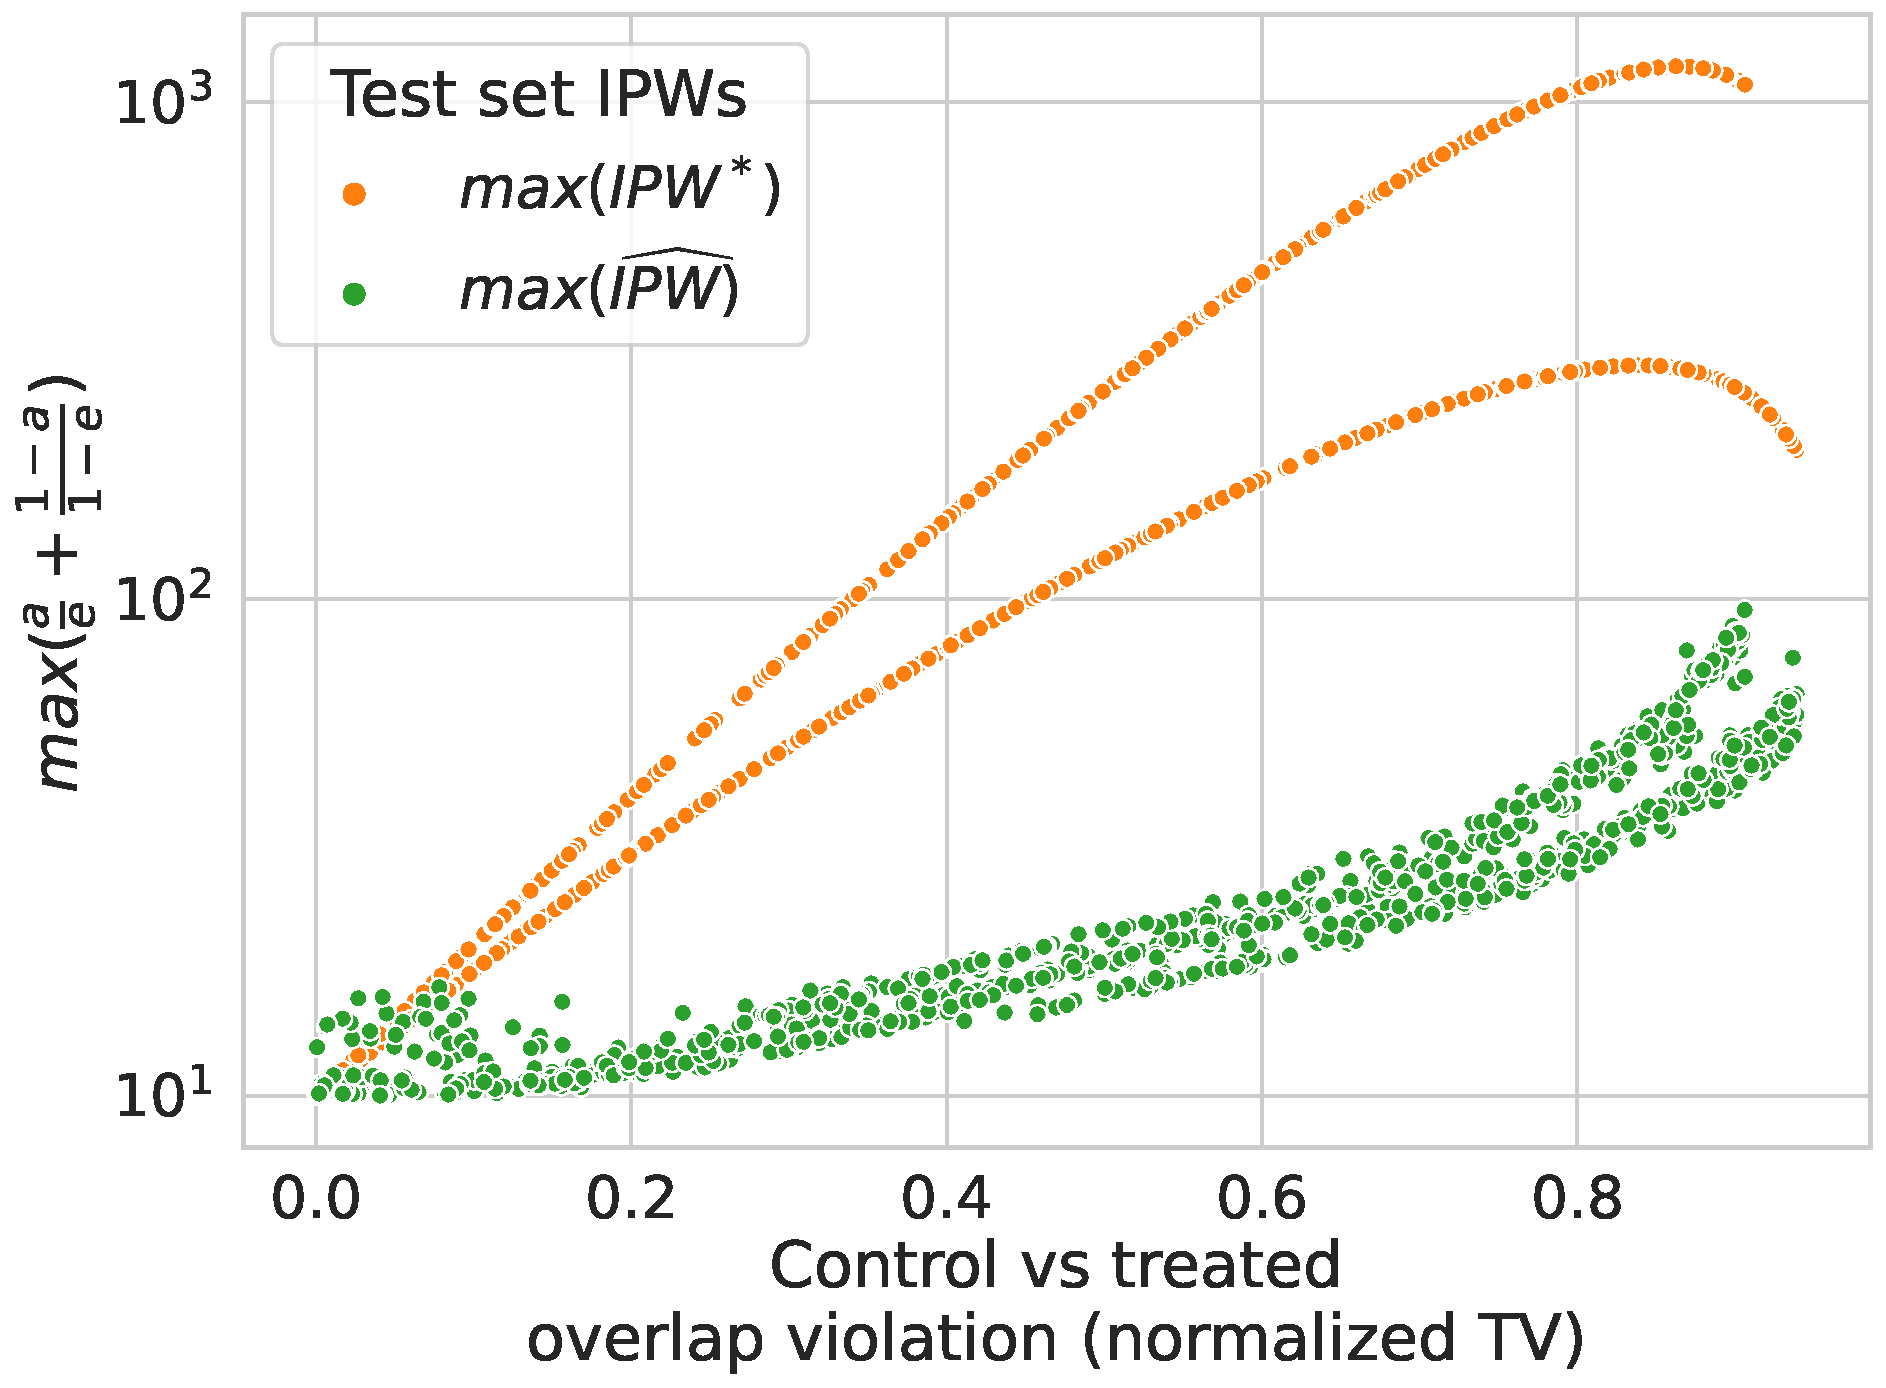
\includegraphics[width=\textwidth]{overlap_measure_caussim_max_ipw_vs_ntv.pdf}
            \label{apd:caussim:max_ipw_vs_ntv}
        \end{subfigure}
        \hfill
        \begin{subfigure}[b]{0.47\textwidth}
            \centering
            \caption{\textbf{ACIC 2016}}
            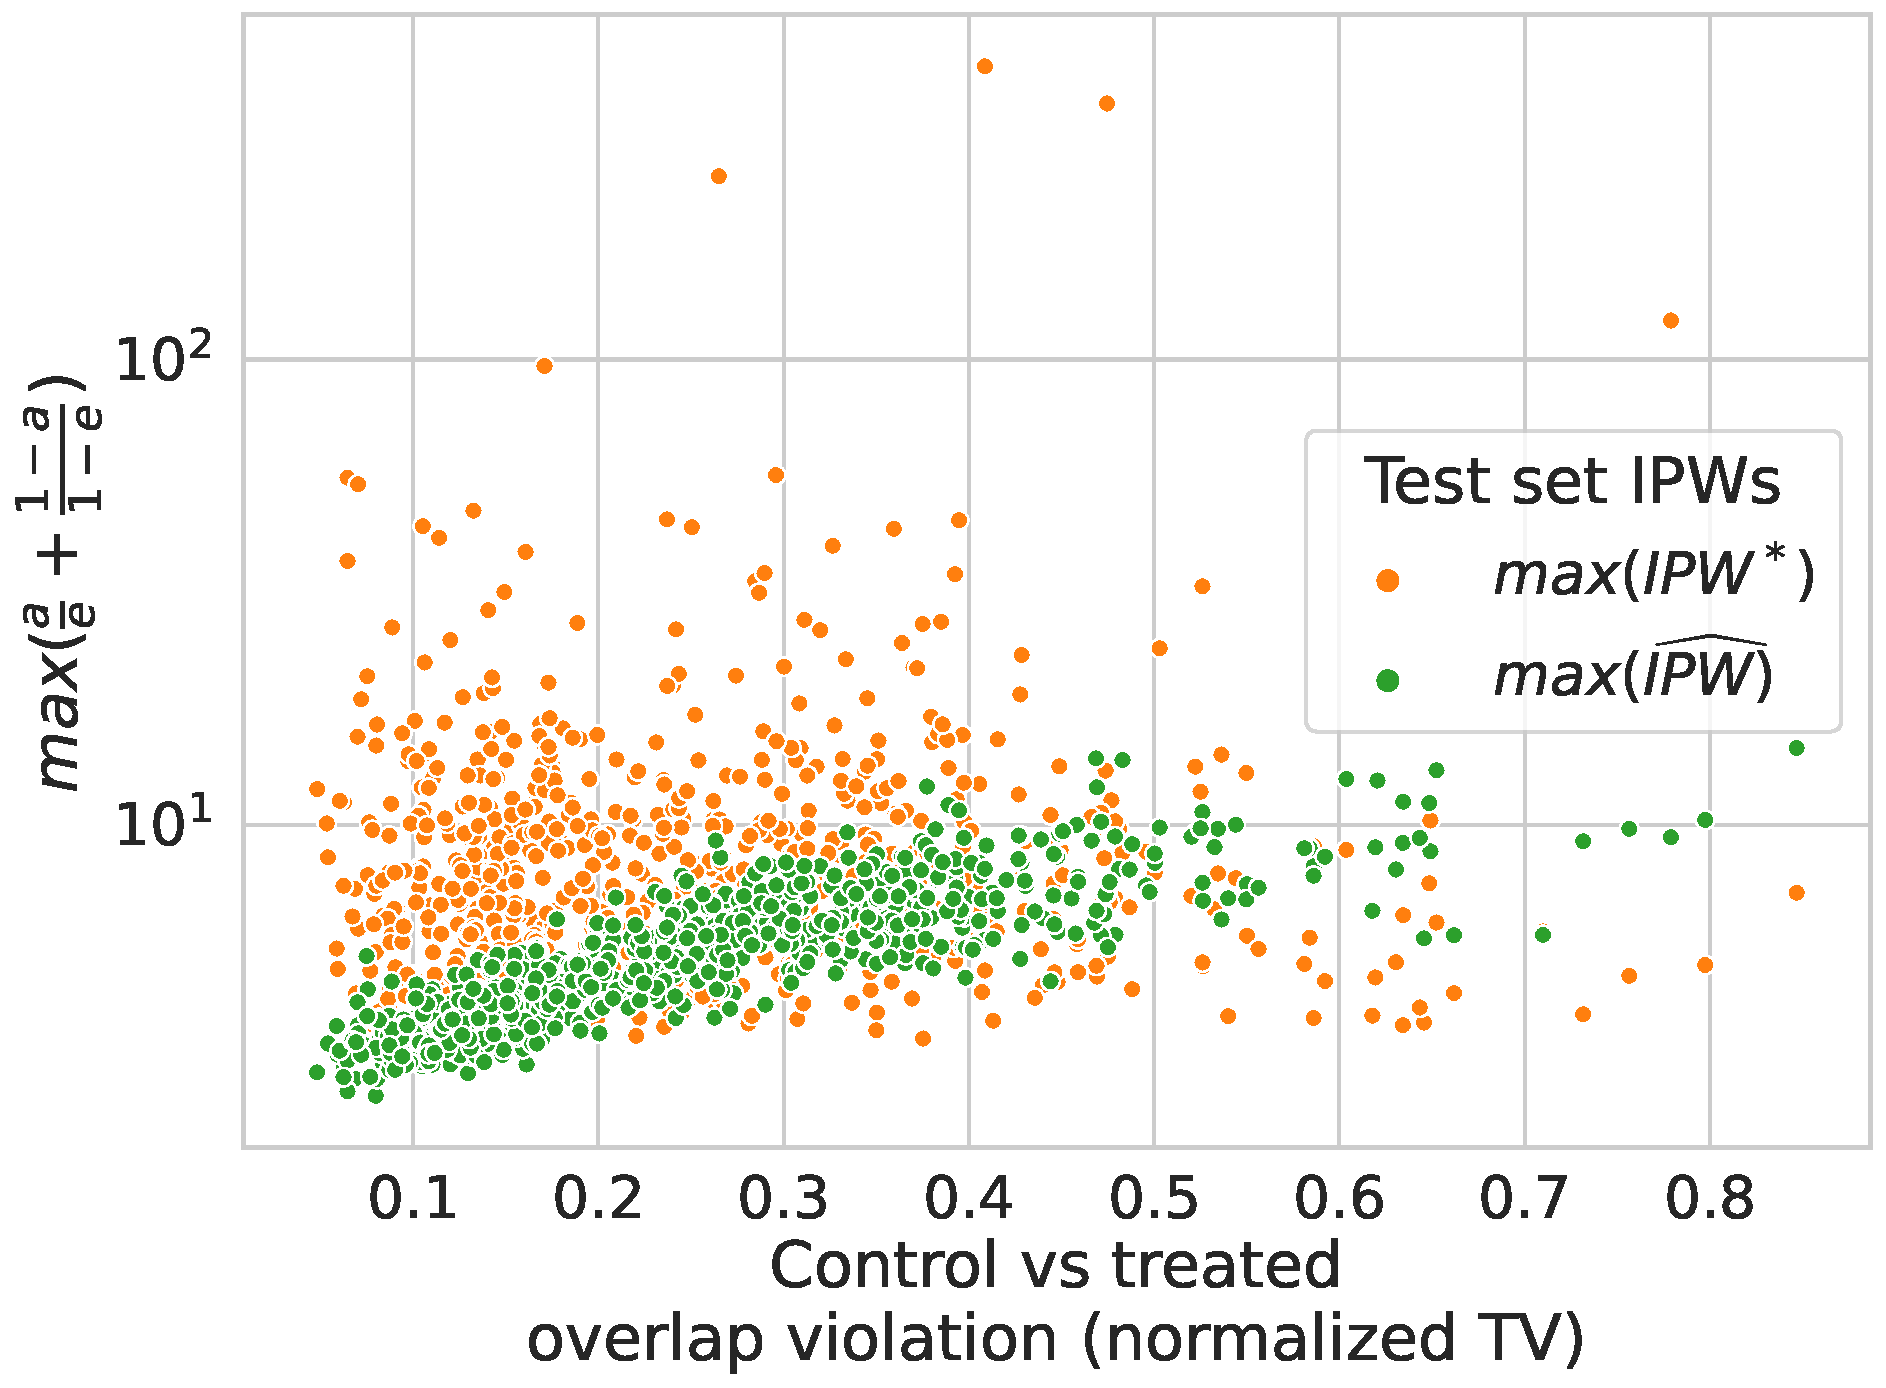
\includegraphics[width=\textwidth]{overlap_measure_acic_2016_max_ipw_vs_ntv.pdf}
            \label{apd:acic_2016:ntv_vs_max_ipw}
        \end{subfigure}
        \begin{subfigure}[b]{0.47\textwidth}
            \centering
            \caption{\textbf{ACIC 2018}}
            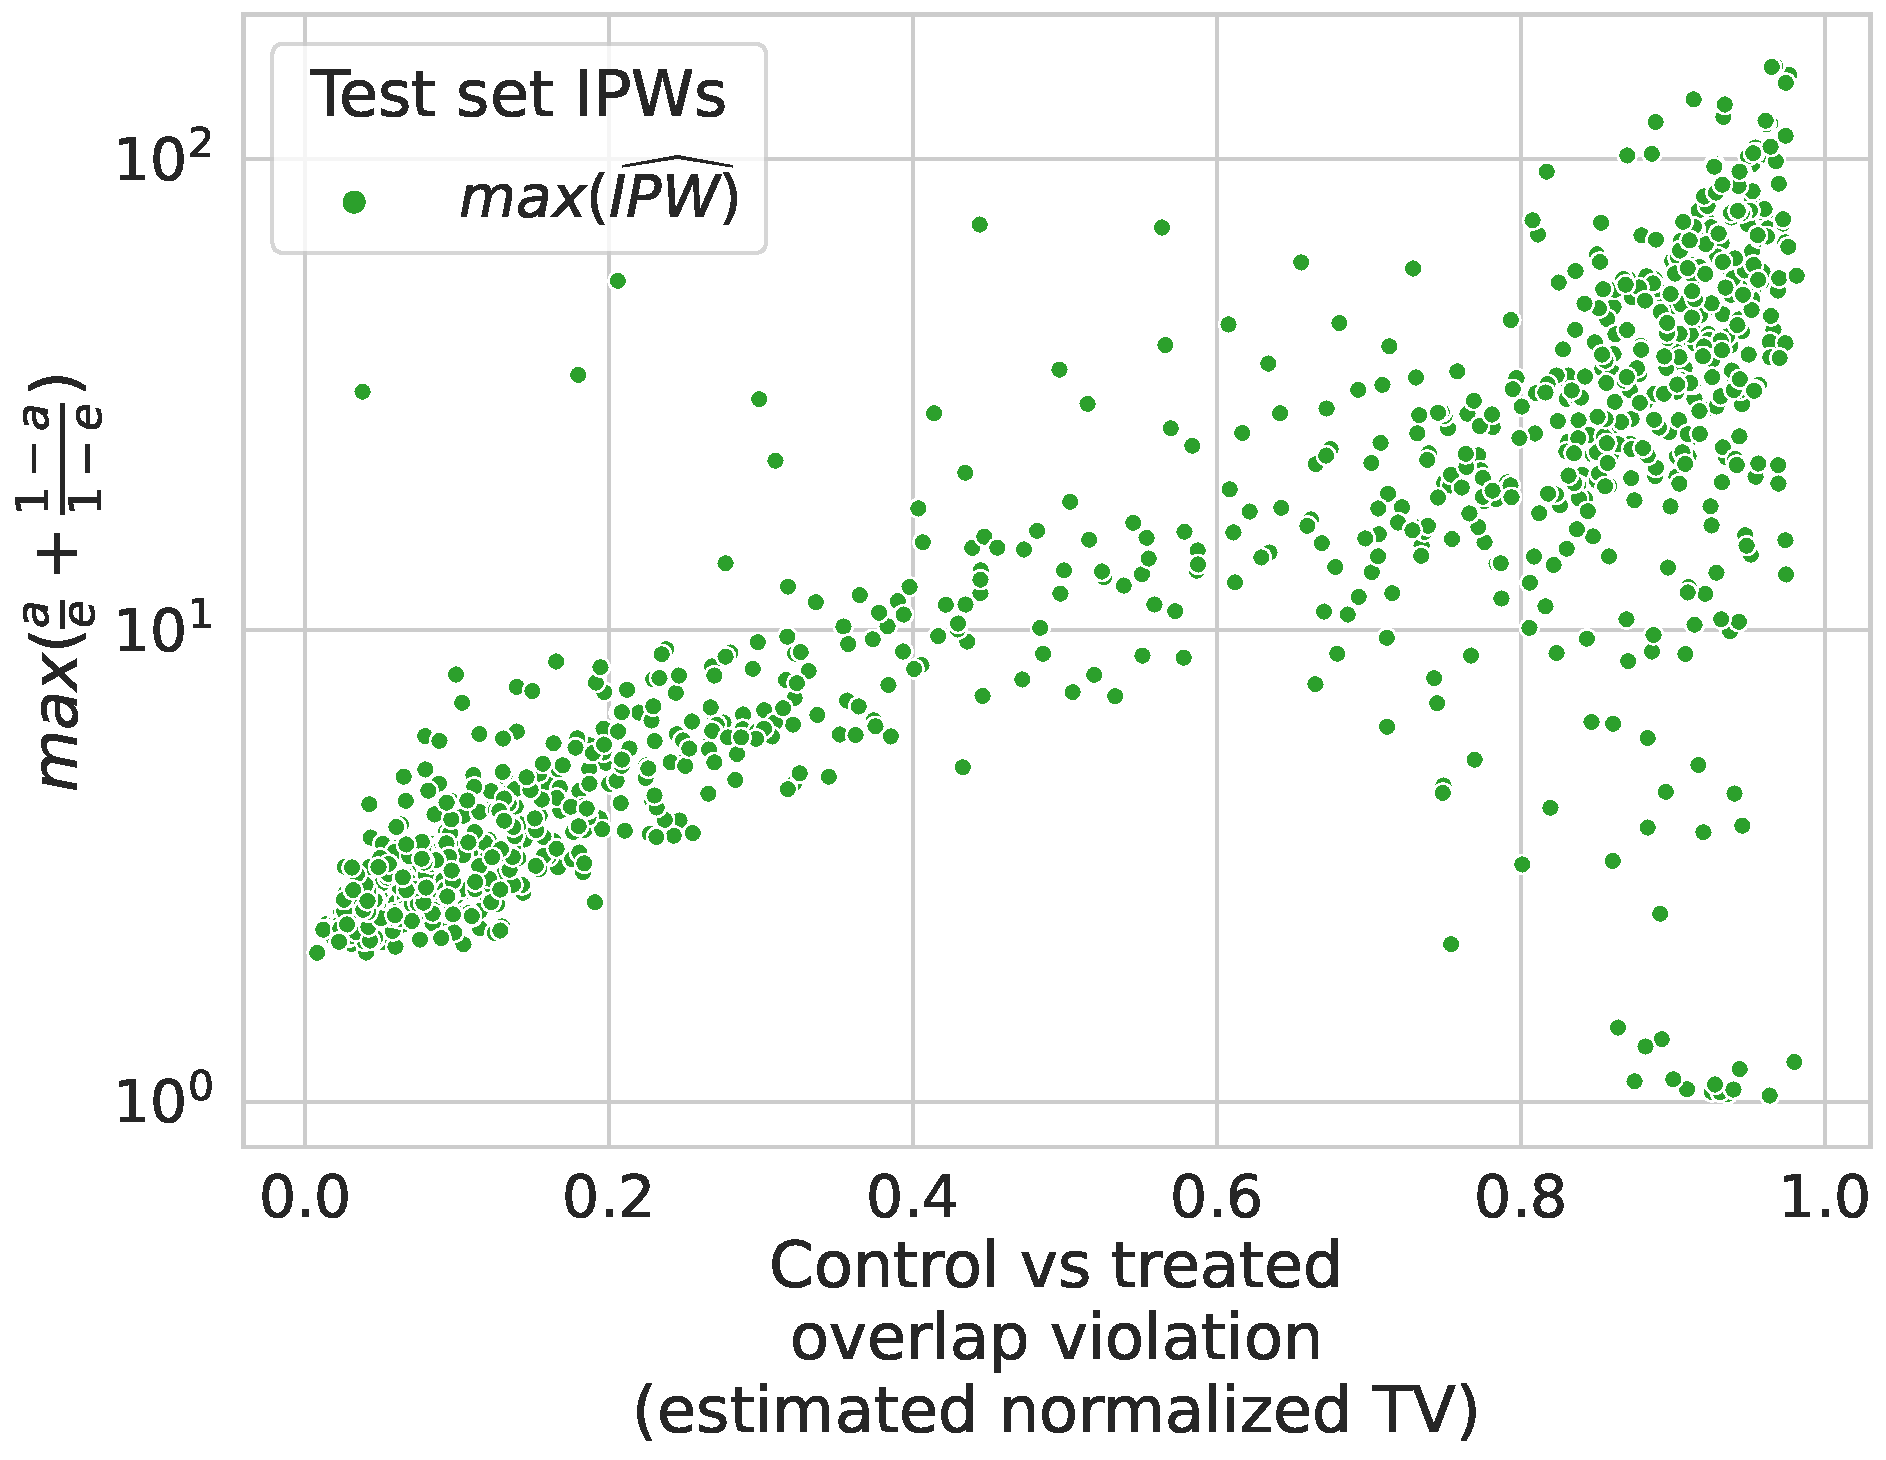
\includegraphics[width=\textwidth]{overlap_measure_acic_2018_max_ipw_vs_ntv.pdf}
            \label{apd:acic_2018:ntv_vs_max_ipw}
        \end{subfigure}
        \hfill
        \begin{subfigure}[b]{0.49\textwidth}
            \centering
            \caption{\textbf{TWINS}}
            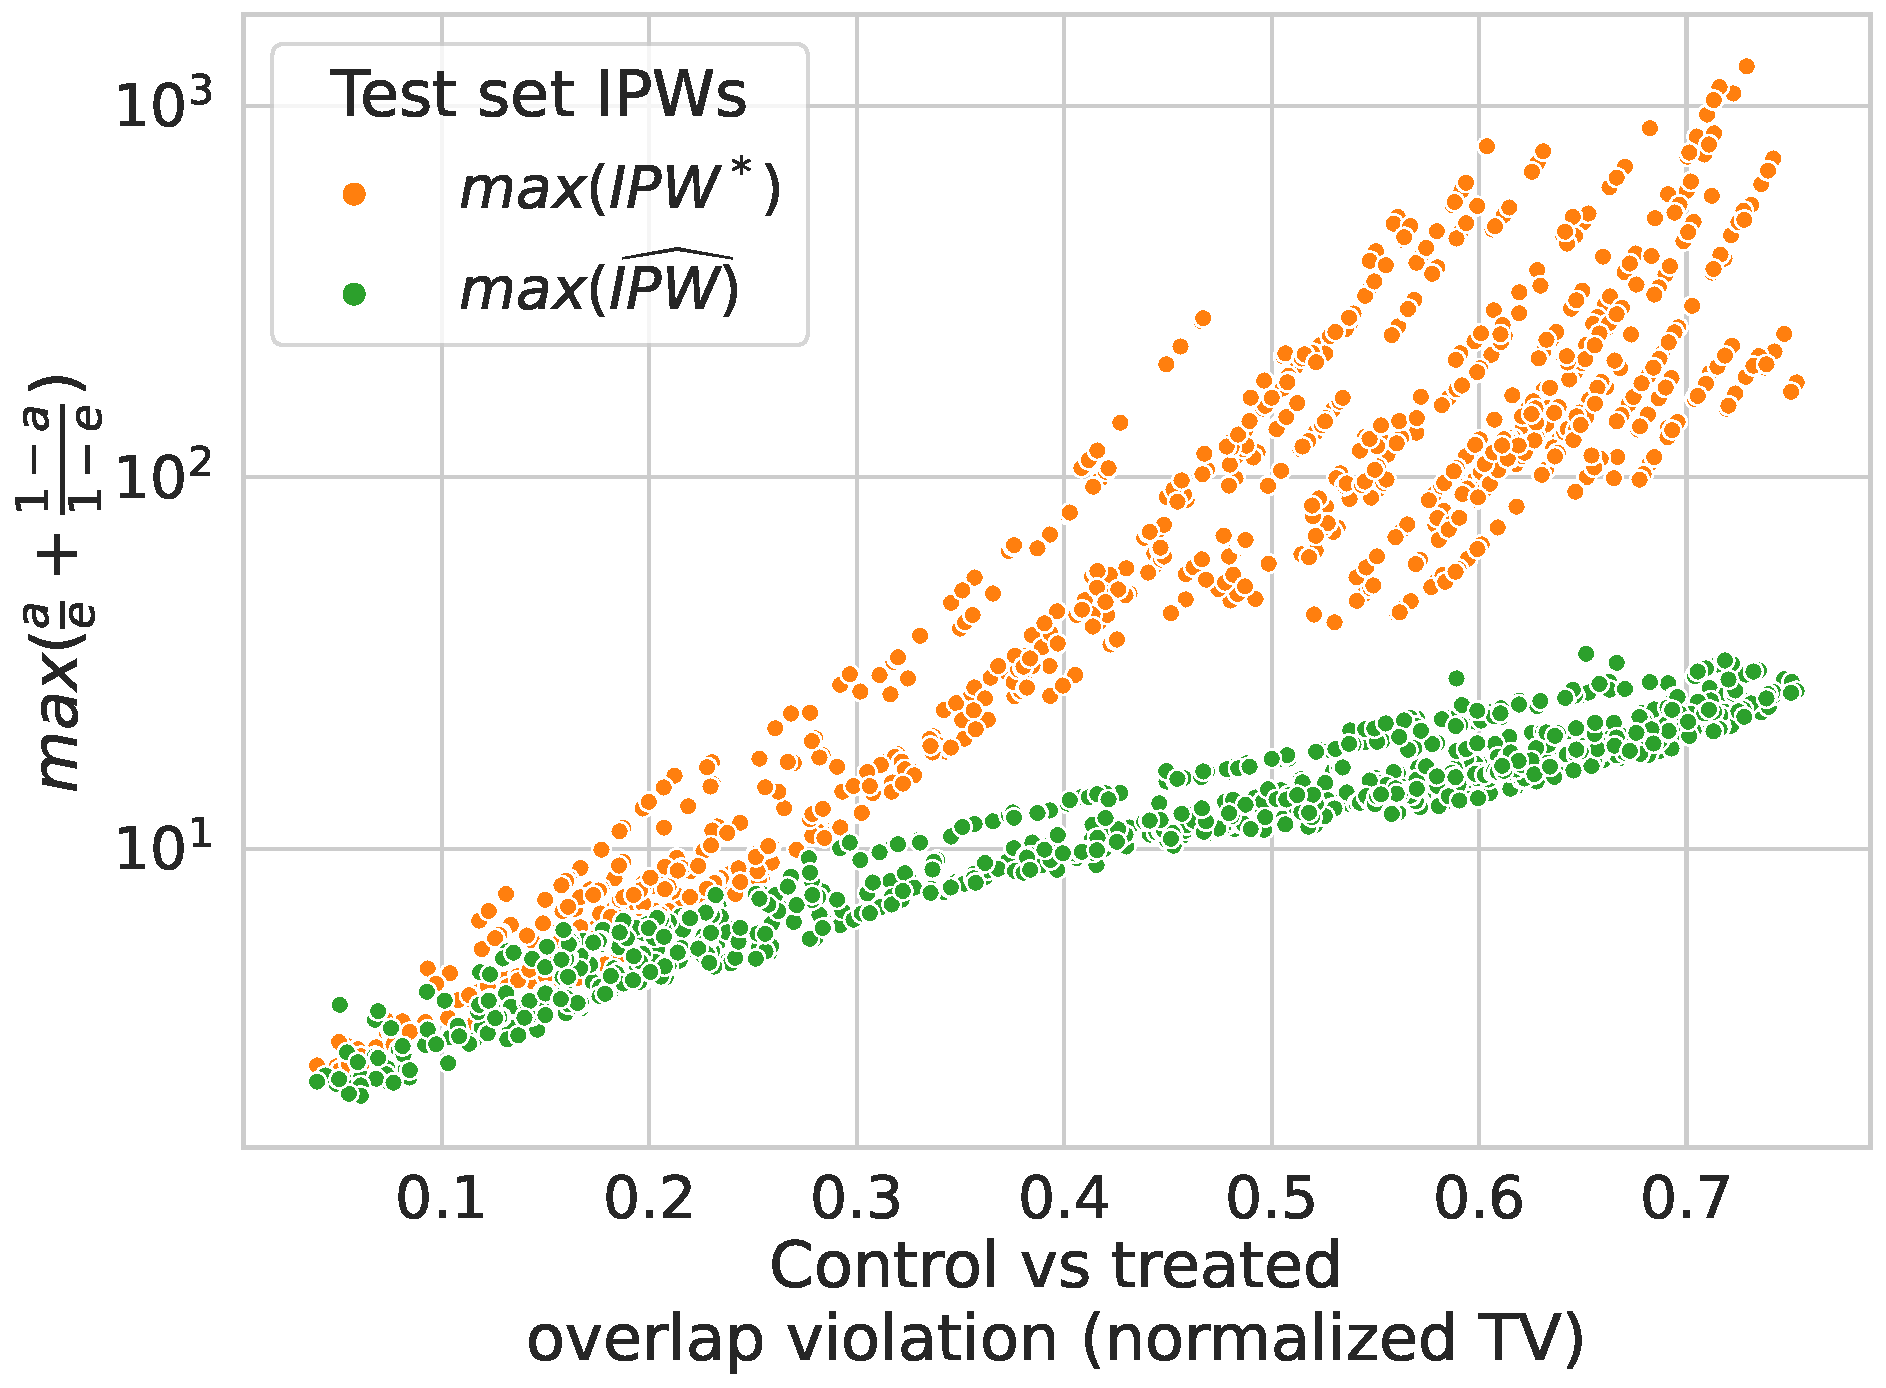
\includegraphics[width=\textwidth]{overlap_measure_twins_max_ipw_vs_ntv.pdf}
            \label{apd:twins:ntv_vs_max_ipw}
        \end{subfigure}
        \caption{Maximal value of Inverse Propensity Weights increases exponentially with the overlap as measure by Normalized Total Variation.}
        \label{apd:ntv_vs_max_ipw}
    \end{figure}


    \section{Experiments}

    \subsection{Details on the data generation process}
    \label{apd:experiments:generation}

    We use Gaussian-distributed covariates and random basis expansion based on
    Radial Basis Function kernels. A random basis of RBF kernel enables modeling
    non-linear and complex relationships between covariates in a similar way to the
    well known spline expansion. The estimators of the response function are learned
    with a linear model on another random basis (which can be seen as a stochastic
    approximation of the full data kernel \cite{rahimi_random_2008}). We carefully
    control the amount of overlap between treated and control populations, a crucial
    assumption for causal inference. Figure \ref{fig:simulation_examples}
    illustrates 2D examples of the simulation.

    \begin{itemize}
        \item The raw features for both populations are drawn from a mixture of
              Gaussians:
              $\mathbb P(X) = p_A \mathbb P(X|A=1) + (1- p_A) \mathbb P(X|A=0)$
              where $\mathbb P(x|A=a)$ is a rotated Gaussian:
              \begin{equation}
                  \mathbb P(x|A=a) = W \cdot \mathcal N \Big( \begin{bmatrix} (1-2a) \theta \\ 0\end{bmatrix} ; \begin{bmatrix} \sigma_0 & 0 \\ 0 & \sigma_1\end{bmatrix} \Big)
              \end{equation}
              with $\theta$ a parameter controlling overlap (bigger yields poorer
              overlap), $W$ a random rotation matrix and $\sigma_0^2=2;\sigma_1^2=5$.

              This generation process allows to analytically compute the oracle
              propensity scores $e(x)$, to simply control for overlap with the
              parameter $\theta$, the distance between the two Gaussian main axes and
              to  visualize response surfaces.

        \item A basis expansion of the raw features increases the problem dimension.
              Using Radial Basis Function (RBF) Nystroem transformation \footnote{We
                  use the
                  \href{https://scikit-learn.org/stable/modules/generated/sklearn.kernel_approximation.Nystroem.html}{Sklearn
                      implementation, \cite{pedregosa_scikitlearn_2011}}}, we expand the raw
              features into a transformed space. The basis expansion samples
              randomly a small number of representers in the raw data. Then,  it
              computes an approximation of the full N-dimensional kernel with these
              basis components, yielding the transformed features $z(x)$. The number
              of basis functions --\emph{ie. knots}--, controls the complexity of
              the ground-truth response surfaces and treatment. We first use this
              process to draw the non-treated response surface $\mu_0$ and the
              causal effect $\tau$. We then draw the observations from a mixture two
              Gaussians, for the treated and non treated. We vary the separation
              between the two Gaussians to control the overlap between treated and
              non-treated populations, an important parameter for causal inference
              (related to $\eta$ in Proposition
              \ref{theory:prop:mu_risk_ipw_bound}). Finally, we generate observed
              outcomes adding Gaussian noise.

              More formally, we generate the basis following the original data
              distribution, $\left [ b_1 .. b_D \right ] \sim \mathbb P(x)$,
              with D=2 in our simulations. Then, we compute an approximation
              of the full kernel of the data generation process $RBF(x,
                  \cdot) \;  with \; x \sim \mathbb P(x)$ with these
              representers: $z(x) = [RBF_{\gamma}(x, b_d)]_{d=1..D} \cdot
                  Z^T \in \mathbb{R}^D$ with $RBF_{\gamma}$ being the Gaussian
              kernel $K(x, y) = exp(-\gamma ||x-y||^2)$ and Z the
              normalization constant of the kernel basis, computed as the
              root inverse of the basis kernel $Z=[K(b_i, b_j)]_{i, j \in
                  {1..D}}^{-1/2}$


        \item Functions $\mu_0$, $\tau$ are distinct linear functions of the
              transformed features:
              \begin{equation*}
                  \mu_0(x) = \begin{bmatrix} z(x); 1 \end{bmatrix} \cdot \beta_{\mu}^T
              \end{equation*}
              \begin{equation*}
                  \tau(x) = \begin{bmatrix} z(x); 1 \end{bmatrix} \cdot \beta_{\tau}^T
              \end{equation*}
        \item Adding a Gaussian noise, $\varepsilon \sim \mathcal N(0, \sigma(x;a))$,
              we construct the potential outcomes:
              $y(a) = \mu_0(x) + a\,\tau(x) + \varepsilon(x, a)$
    \end{itemize}
    We generated 1000 instances of this dataset with uniformly random overlap
    parameters $\theta \in \left[ 0, 2.5 \right]$.

    \begin{figure}[!t]
        \centering
        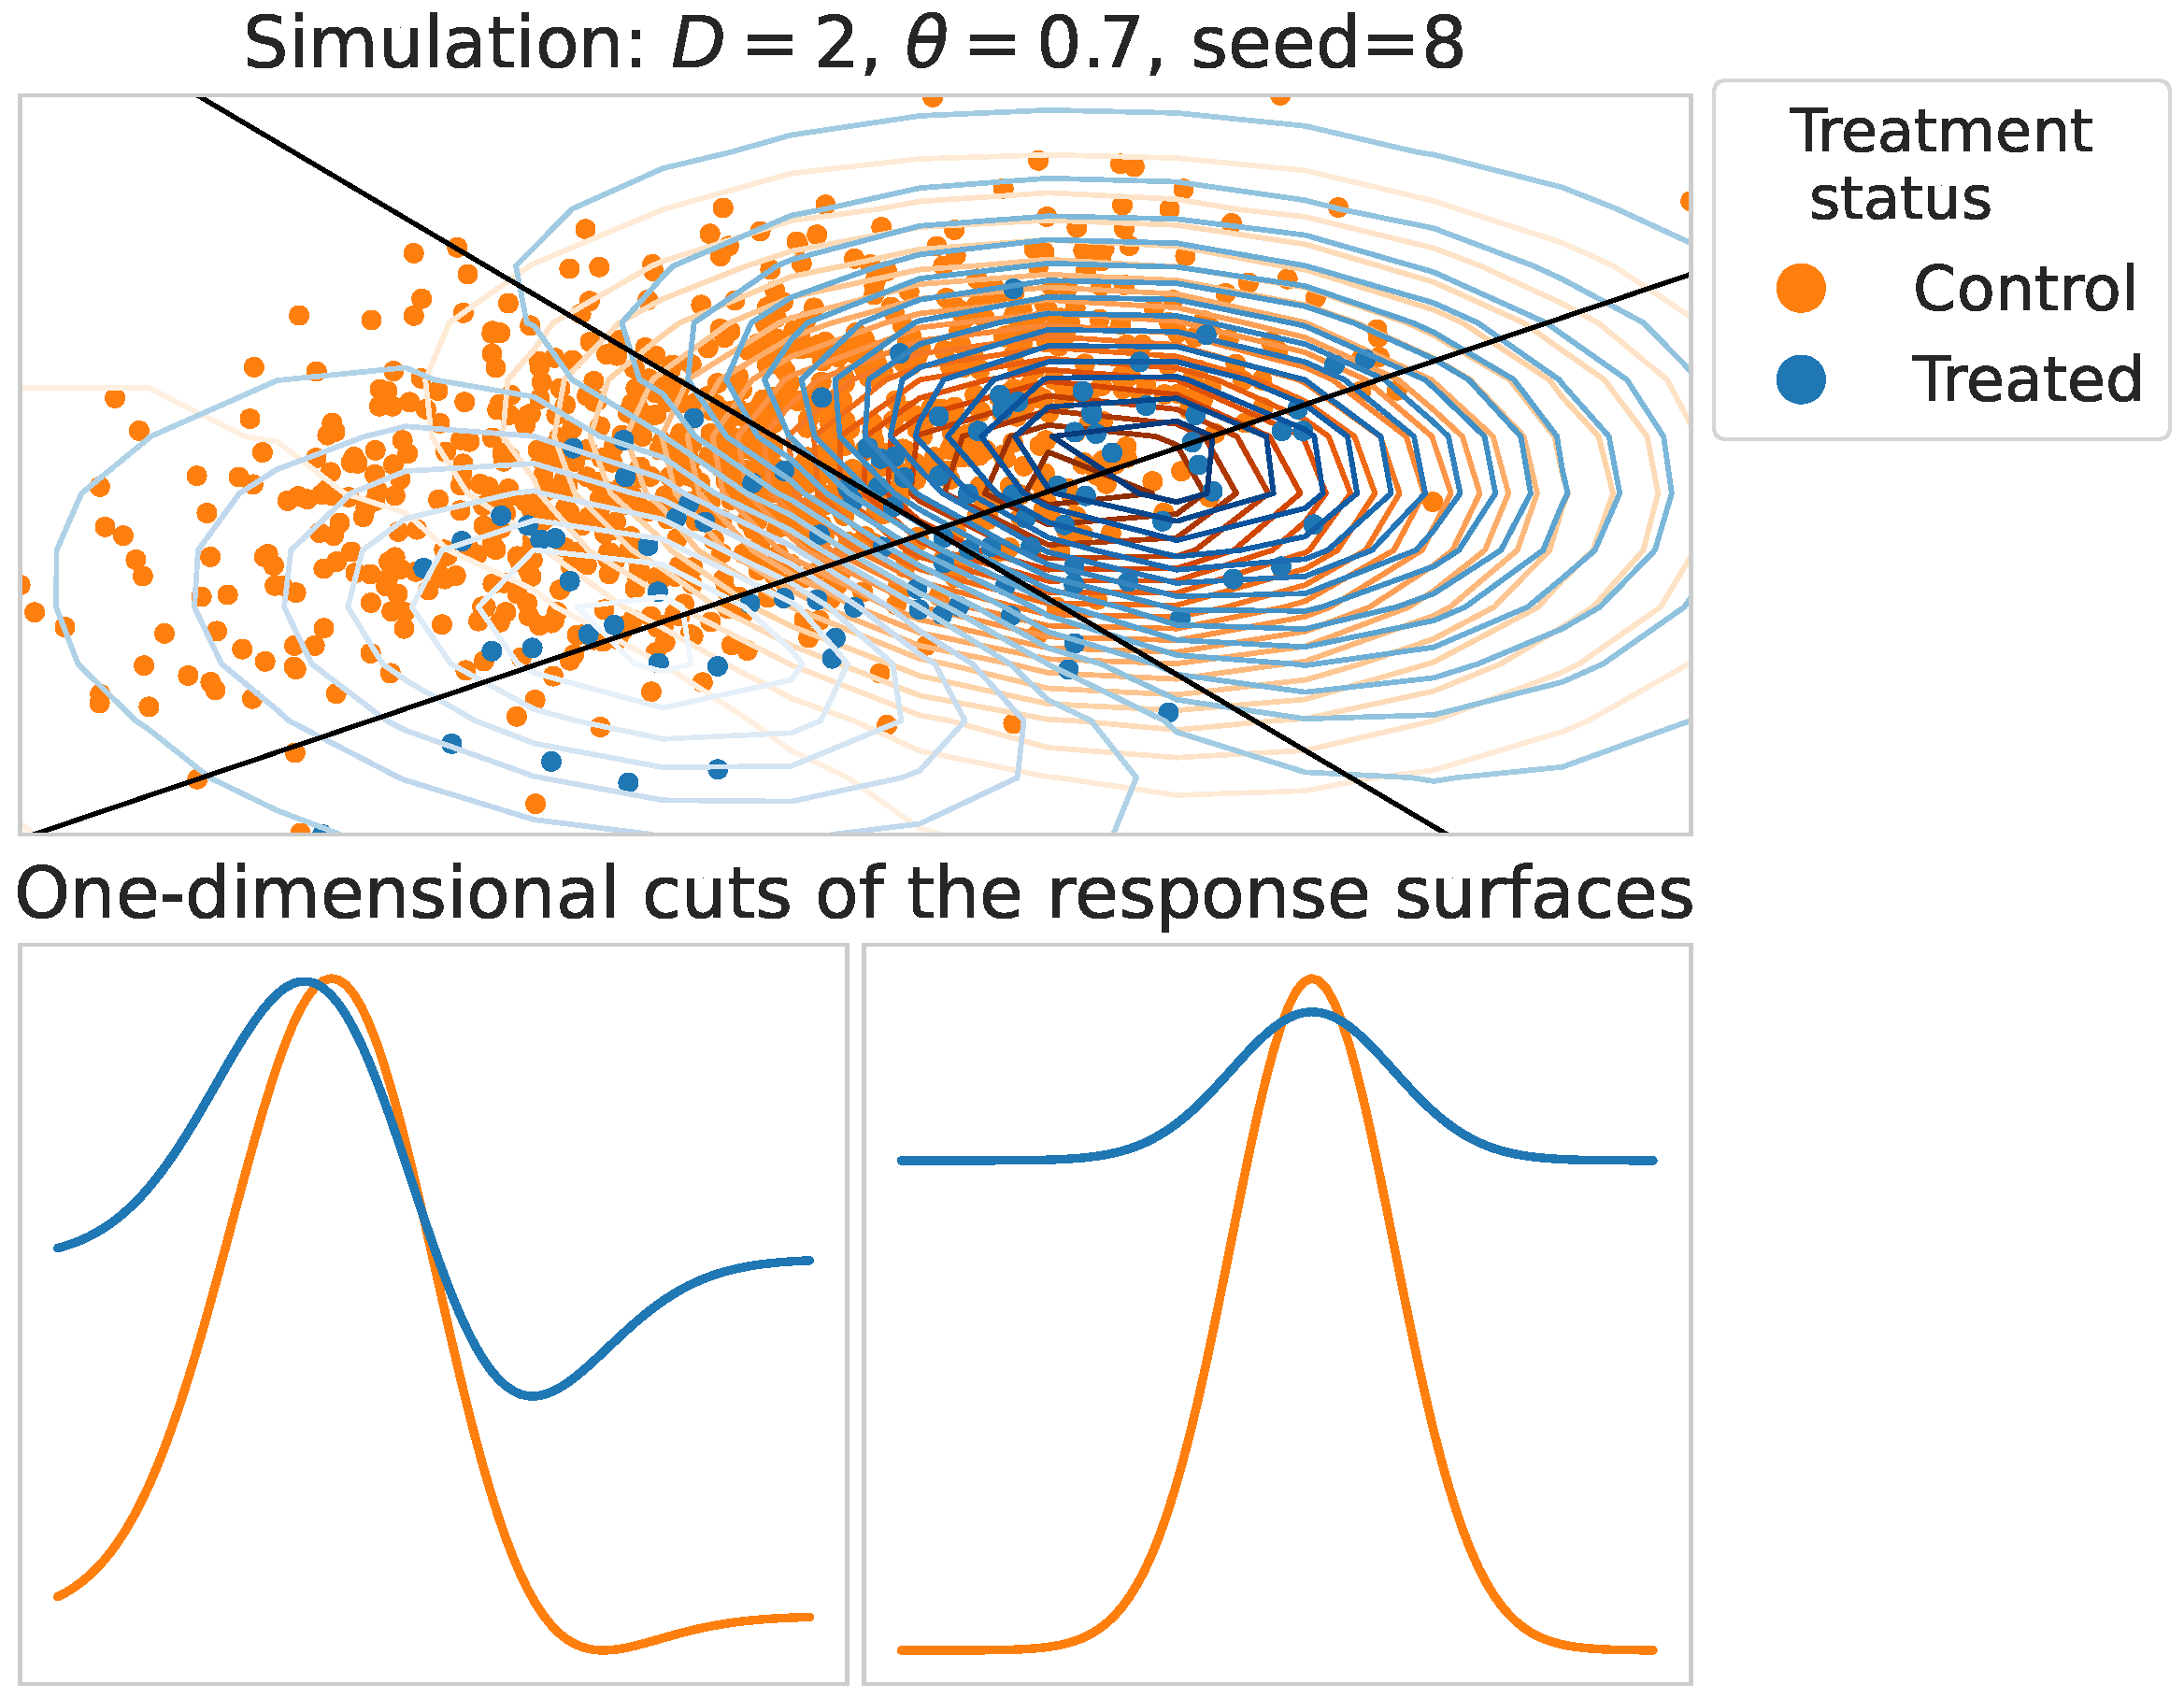
\includegraphics[width=0.8\linewidth]{caussim_example_rs_gaussian=8_rs_rotation=8_ntv=0.37_D=2_overlap=0.7_p_A=0.1.pdf}

        \caption{Example of the simulation setup in the input space with two
            knots --\emph{ie.} basis functions. The top panel
            shows the observations in feature space, while the bottom panel displays the
            two response surfaces on a 1D cut along the black lines drawn on
            the top panel.}
        \label{fig:simulation_examples}
    \end{figure}


    \subsection{ Details on the semi-simulated datasets}\label{apd:experiments:datasets}


    \begin{itemize}
        \item[ACIC 2018] \cite{dorie_automated_2019}:  The initial intervention was a child’s birth
            weight $(A = 1 \text{ if weight} < 2.5 kg)$, and outcome was the child’s
            IQ after a follow-up period. The study contained $N=4\,802$ data
            points with $D=55$ features (5 binary, 27 count data, and 23
            continuous). They simulated 77 different setups varying parameters
            for treatment and response models, overlap, and interactions between treatment and
            covariates \footnote{Original R code available at
                \url{https://github.com/vdorie/aciccomp/tree/master/2016}
                to generate 77 simulations settings.}. We used 10 different seeds
            for each setup, totaling 770 dataset instances.

        \item[ACIC 2018] \cite{shimoni_benchmarking_2018}: Starting from data from
            the Linked Births and Infant Deaths Database (LBIDD)
            \cite{macdorman_infant_1998} with $D=177$ covariates, treatment and
            outcome models are simulated with complex models to reflect different
            scenarii. The data do not provide the true propensity scores, so we
            evaluate only feasible metrics, which do not require this nuisance
            parameter. We used all 432 datasets\footnote{Using the scaling part of
                the data, from
                \href{https://github.com/IBM-HRL-MLHLS/IBM-Causal-Inference-Benchmarking-Framework}{github.com/IBM-HRL-MLHLS/IBM-Causal-Inference-Benchmarking-Framework}}
            of size $N=5\,000$.


        \item[Twins] \cite{louizos_causal_2017}: It is an augmentation of
            real data on twin births and mortality rates
            \cite{almond_costs_2005}. There are $N=11\,984$ samples (pairs of twins),
            and $D=50$ covariates\footnote{We obtained the dataset from
                \href{https://github.com/AMLab-Amsterdam/CEVAE/tree/master/datasets/TWINS}{https://github.com/AMLab-Amsterdam/CEVAE/tree/master/datasets/TWINS}}, The outcome is the mortality and the treatment is the
            weight of the heavier twin at birth. This is a "true" counterfactual dataset
            \cite{curth_really_2021} in the sense that we have
            both potential outcomes with each twin. They simulate the treatment with a
            sigmoid model based on GESTAT10 (number of gestation weeks before birth) and x
            the 45 other covariates:
            \begin{align}
                \mathbf{t}_{i} & \mid \mathbf{x}_{i}, \mathbf{z}_{i} \sim
                \operatorname{Bern}\left(\sigma\left(w_{o}^{\top}
                \mathbf{x}+w_{h}(\mathbf{z} / 10-0.1)\right)\right)       \\ & \text{with} \;
                w_{o} \sim \mathcal{N}(0,0.1 \cdot I),\; w_{h} \sim \mathcal{N}(5,0.1) \nonumber
            \end{align}
            We add a non-constant slope in the
            sigmoid to control the overlap between
            treated and control populations.
            We sampled uniformly 1\,000 different overlap parameters between 0 and
            2.5, totaling 1\,000 dataset instances. Unlike the previous datasets,
            only the overlap varies for these instances. The response surfaces are
            set by the original outcomes.
    \end{itemize}

    \subsection{Model selection procedures}

    \paragraph{Nuisances estimation}\label{apd:experiments:nuisances_hp}

    The nuisances are estimated with a stacked regressor inspired by the Super
    Learner framework, \cite{laan_super_2007}). We select hyper-parameters
    with randomized search on a validation set $\mathcal{V}$ and keep them fix for
    model selection  The searc grid is detailed in Table
    \ref{apd:experiments:nuisances_hp_grid}. All implementations come from
    \href{https://scikit-learn.org/stable/}{scikit-learn}
    \cite{pedregosa_scikitlearn_2011}.  As extreme inverse propensity weights induce
    high variance, we use clipping \cite{swaminathan_counterfactual_2015,
        ionides_truncated_2008} to bound $min(\check e, 1-\check e)$ away from 0 with a
    fixed $\eta=10^{-10}$, ensuring strict overlap for numerical stability.

    \begin{table}[h!]
        \begin{tabular}{llll}
            \toprule
            Model                & Estimator
                                 & Hyper-parameters grid                                         \\
            \midrule
            Outcome, m           & StackedRegressor
                                 & ridge regularization: [0.0001, 0.001, 0.01, 0.1, 1, 10, 100]  \\
            \multirow[c]{3}{*}{} & (HistGradientBoostingRegressor, ridge)
                                 & HistGradientBoostingRegressor  learning rate: [0.01, 0.1, 1]  \\
                                 &
                                 & HistGradientBoostingRegressor  max leaf nodes: [10,
            20, 30, 50]                                                                          \\
            \midrule
            Treatment, e         & StackedClassifier
                                 & LogisticRegression  C: [0.0001, 0.001, 0.01, 0.1, 1, 10, 100] \\
            \multirow[c]{3}{*}{} & (HistgradientBoostingClassifier, LogisticRegression)
                                 & HistGradientBoostingClassifier  learning rate: [0.01, 0.1, 1] \\
                                 &
                                 & HistGradientBoostingClassifier  max leaf nodes: [10,
            20, 30, 50]                                                                          \\
            \bottomrule
        \end{tabular}
        \caption{Hyper-parameters grid used for nuisance models}
        \label{apd:experiments:nuisances_hp_grid}
    \end{table}


    \subsection{Additional Results}\label{apd:experiments:additional_results}

    \paragraph{Definition of the Kendall's tau, $\kappa$}

    The Kendall's tau  is a widely used statistics to measure the rank correlation
    between two set of observations. It measures the number of concordant pairs
    minus the discordant pairs normalized by the total number of pairs. It takes values in the
    $[-1, 1]$ range.
    \begin{equation}\label{eq:kendall_tau}
        \kappa=\frac{\text { (number of concordant pairs })-\text { (number of discordant pairs) }}{\text { (number of pairs) }}
    \end{equation}

    \paragraph{Values of relative $\kappa(\ell,\tau\mathrm{{-risk}})$ compared to
        the mean over all metrics Kendall's as shown in the boxplots of Figure \ref{fig:relative_kendalls_all_datasets}}

    \begin{table}
        \centering
        \resizebox{0.7\textwidth}{!}{
            \begin{tabular}{llrrrr}
    \toprule
                                                                 &           &
    \multicolumn{2}{r}{Strong
    Overlap}                                                     &
    \multicolumn{2}{r}{Weak
        Overlap}
    \\ \midrule
                                                                 &           & Median & IQR   & Median & IQR \\
    Metric                                                       & Dataset   &        &       &        &     \\
    \midrule
    \multirow[c]{4}{*}{$\widehat{\mu\mathrm{-risk}}$}            & Twins
    (N=11 984)                                                   & -0.32     & 0.12   & -0.19 & 0.12         \\
    \cline{2-6}
                                                                 & ACIC 2016
    (N=4 802)                                                    & -0.03     & 0.13   & 0.11  & 0.19         \\
    \cline{2-6}
                                                                 & Caussim
    (N=5 000)                                                    & -0.40     & 0.55   & -0.16 & 0.31         \\
    \cline{2-6}
                                                                 & ACIC 2018
    (N=5 000)                                                    & 0.00      & 0.30   & 0.01  & 0.40         \\
    \cline{1-6} \cline{2-6}
    \multirow[c]{4}{*}{$\widehat{\mu\mathrm{-risk}}_{IPW}$}      & Twins
    (N= 11 984)                                                  & -0.31     & 0.13   & -0.17 & 0.12         \\
    \cline{2-6}
                                                                 & ACIC 2016
    (N=4 802)                                                    & -0.02     & 0.13   & 0.11  & 0.19         \\
    \cline{2-6}
                                                                 & Caussim
    (N=5 000)                                                    & -0.34     & 0.50   & 0.09  & 0.31         \\
    \cline{2-6}
                                                                 & ACIC 2018
    (N=5 000)                                                    & 0.00      & 0.30   & -0.01 & 0.43         \\
    \cline{1-6} \cline{2-6}
    \multirow[c]{3}{*}{$\widehat{\mu\mathrm{-risk}}^{*}_{IPW}$}  & Twins
    (N= 11 984)                                                  & -0.32     & 0.13   & -0.17 & 0.13         \\
    \cline{2-6}
                                                                 & ACIC 2016
    (N=4 802)                                                    & -0.02     & 0.13   & 0.11  & 0.21         \\
    \cline{2-6}
                                                                 & Caussim
    (N=5 000)                                                    & -0.33     & 0.54   & 0.26  & 0.27         \\
    \cline{1-6} \cline{2-6}
    \multirow[c]{4}{*}{$\widehat{\tau\mathrm{-risk}}_{IPW}$}     & Twins
    (N= 11 984)                                                  & 0.13      & 0.12   & 0.27  & 0.12         \\
    \cline{2-6}
                                                                 & ACIC 2016
    (N=4 802)                                                    & -0.07     & 0.18   & 0.05  & 0.31         \\
    \cline{2-6}
                                                                 & Caussim
    (N=5 000)                                                    & -0.19     & 0.43   & -0.14 & 0.18         \\
    \cline{2-6}
                                                                 & ACIC 2018
    (N=5 000)                                                    & -0.16     & 0.40   & -0.11 & 0.66         \\
    \cline{1-6} \cline{2-6}
    \multirow[c]{3}{*}{$\widehat{\tau\mathrm{-risk}}_{IPW}^{*}$} & Twins
    (N= 11 984)                                                  & 0.12      & 0.14   & 0.20  & 0.16         \\
    \cline{2-6}
                                                                 & ACIC 2016
    (N=4 802)                                                    & -0.03     & 0.16   & -0.09 & 0.43         \\
    \cline{2-6}
                                                                 & Caussim
    (N=5 000)                                                    & -0.15     & 0.46   & -0.17 & 0.19         \\
    \cline{1-6} \cline{2-6}
    \multirow[c]{4}{*}{$\widehat{\mathrm{U-risk}}$}              & Twins
    (N= 11 984)                                                  & 0.13      & 0.12   & 0.02  & 0.25         \\
    \cline{2-6}
                                                                 & ACIC 2016
    (N=4 802)                                                    & 0.04      & 0.11   & 0.11  & 0.26         \\
    \cline{2-6}
                                                                 & Caussim
    (N=5 000)                                                    & 0.04      & 0.43   & -0.04 & 0.17         \\
    \cline{2-6}
                                                                 & ACIC 2018
    (N=5 000)                                                    & 0.12      & 0.26   & -0.02 & 0.50         \\
    \cline{1-6} \cline{2-6}
    \multirow[c]{3}{*}{$\widehat{\mathrm{U-risk}}^{*}$}          & Twins
    (N= 11 984)                                                  & 0.25      & 0.08   & -0.41 & 0.45         \\
    \cline{2-6}
                                                                 & ACIC 2016
    (N=4 802)                                                    & 0.08      & 0.13   & -0.59 & 0.57         \\
    \cline{2-6}
                                                                 & Caussim
    (N=5 000)                                                    & 0.46      & 0.12   & 0.02  & 0.44         \\
    \cline{1-6} \cline{2-6}
    \multirow[c]{4}{*}{$\widehat{\mathrm{R-risk}}$}              & Twins
    (N= 11 984)                                                  & 0.15      & 0.10   & 0.25  & 0.18         \\
    \cline{2-6}
                                                                 & ACIC 2016
    (N=4 802)                                                    & 0.07      & 0.12   & 0.22  & 0.15         \\
    \cline{2-6}
                                                                 & Caussim
    (N=5 000)                                                    & 0.34      & 0.26   & 0.13  & 0.21         \\
    \cline{2-6}
                                                                 & ACIC 2018
    (N=5 000)                                                    & 0.13      & 0.27   & 0.21  & 0.47         \\
    \cline{1-6} \cline{2-6}
    \multirow[c]{3}{*}{$\widehat{\mathrm{R-risk}}^{*}$}          & Twins
    (N= 11 984)                                                  & 0.25      & 0.10   & 0.32  & 0.15         \\
    \cline{2-6}
                                                                 & ACIC 2016
    (N=4 802)                                                    & 0.12      & 0.12   & 0.25  & 0.15         \\
    \cline{2-6}
                                                                 & Caussim
    (N=5 000)                                                    & 0.47      & 0.11   & 0.16  & 0.14         \\
    \cline{1-6} \cline{2-6}
    \bottomrule
\end{tabular}

        }
        \caption{Values of relative $\kappa(\ell,\tau\mathrm{{-risk}})$ compared to
            the mean over all metrics Kendall's as shown in the boxplots of Figure
            \ref{fig:relative_kendalls_all_datasets}}\label{apd:table:relative_kendalls_all_datasets}
    \end{table}


    \paragraph{Figure \ref{apd:fig:relative_kendalls_all_datasets_all_metrics} -
        Results measured in relative Kendall's for feasible and semi-oracle risks}

    Because of extreme propensity scores in the denominator and bayes error residuals in the numerator, the semi-oracle
    $U$-risk has poor performances at bad overlap. Estimating these propensity scores in the is feasible $U$-risk reduces
    the variance since clipping is performed.

    \begin{figure}[!b]
        \centering
        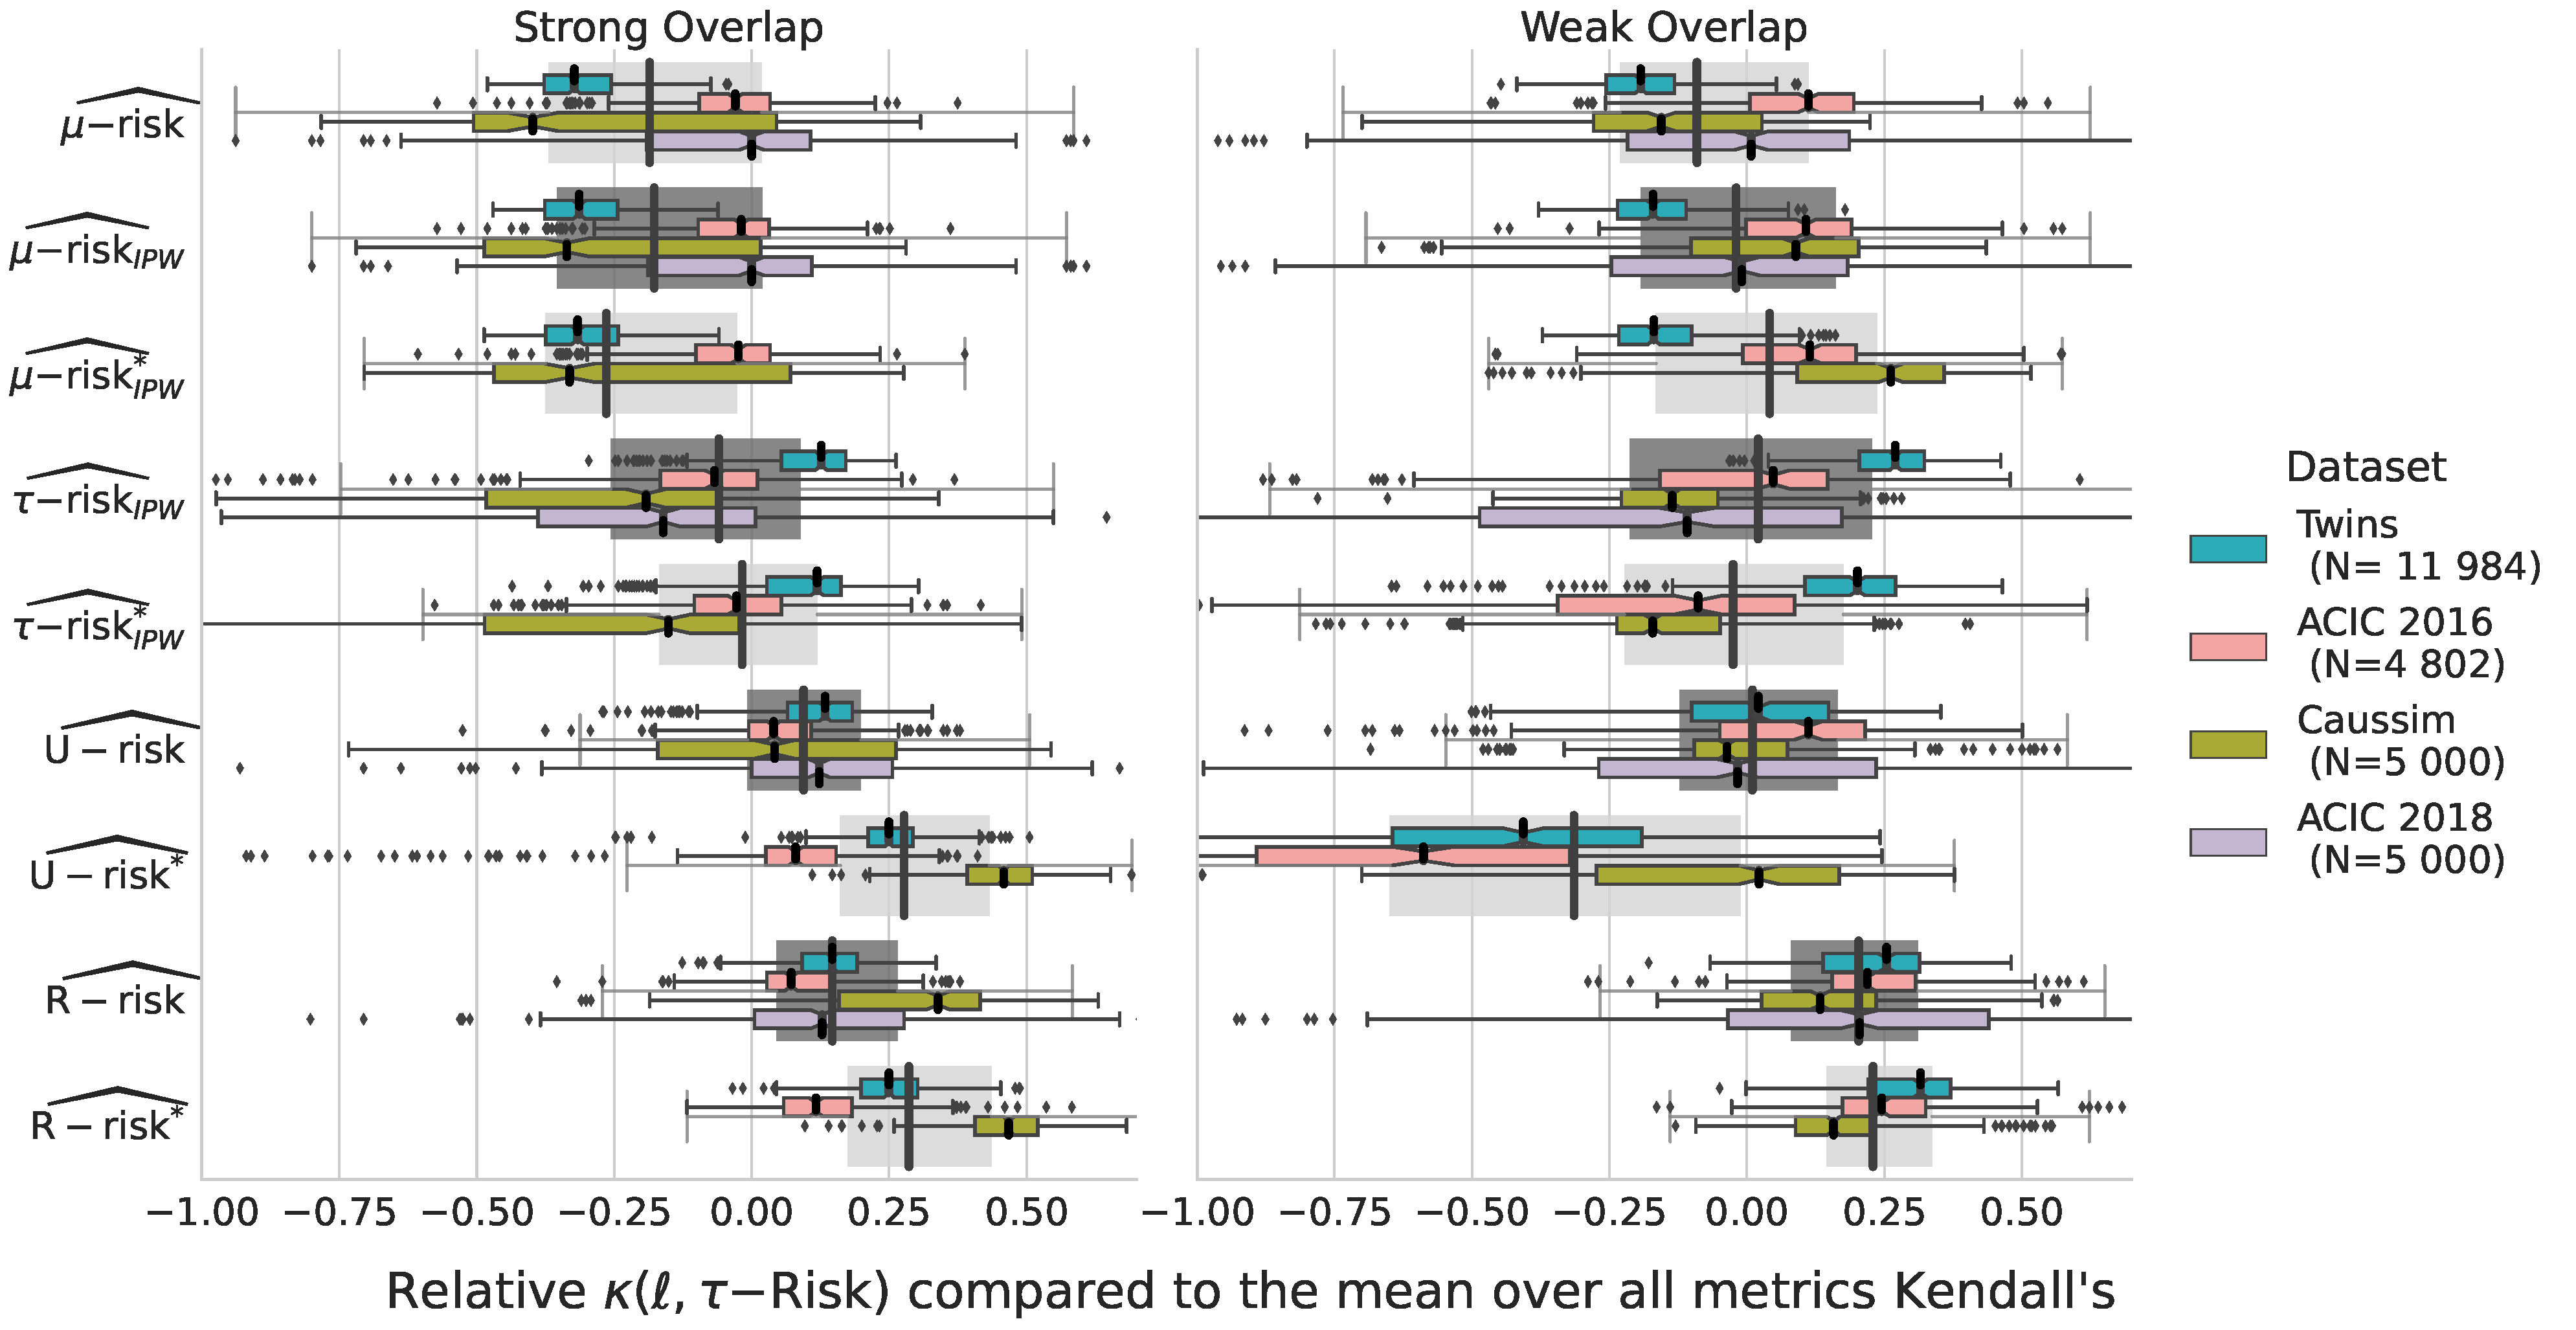
\includegraphics[width=\linewidth]{_1_r_risk_domination_r_risk_domination__ref_metric_mean_risks_by_Dataset.pdf}
        %\hfill
        \caption{\textbf{The $R$-risk is the best metric}: Relative Kendall's $\tau$
            agreement with $\tau\text{-risk}$. Strong and Weak overlap correspond to
            the first and last tertiles of the overlap distribution measured with
            Normalized Total Variation eq. \ref{eq:ntv}.
        }\label{apd:fig:relative_kendalls_all_datasets_all_metrics}
    \end{figure}

    \paragraph{Figure \ref{apd:fig:all_datasets_tau_risk_ranking_agreement} -
        Results measured in absolute Kendall's}


    \begin{figure}
        \centering
        \begin{subfigure}[b]{0.44\textwidth}
            \centering
            \caption{\textbf{Caussim}}
            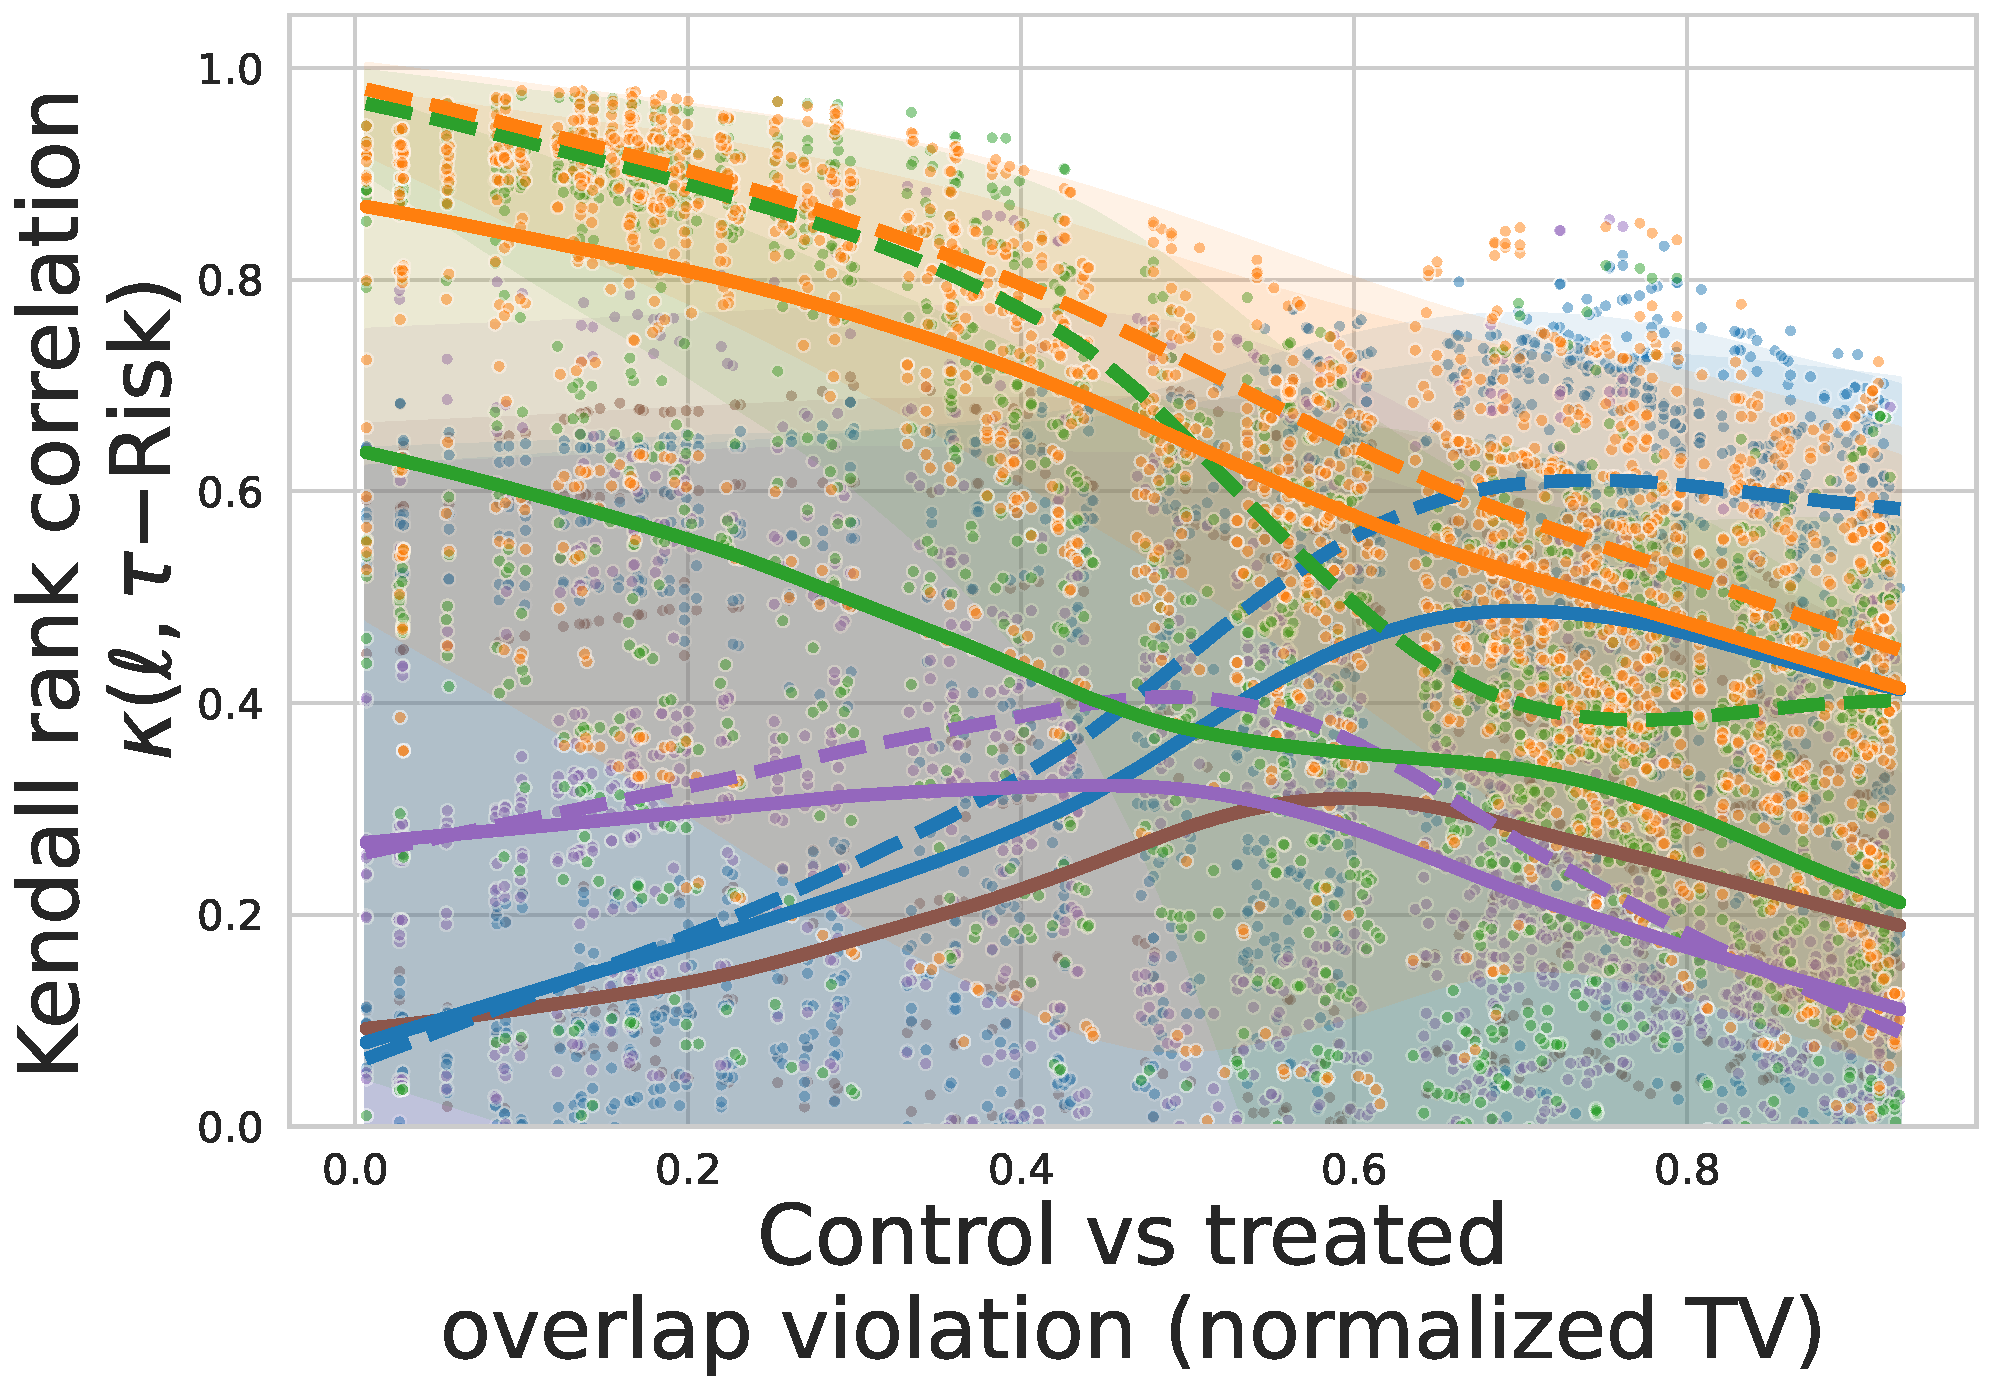
\includegraphics[width=\textwidth]{kendalls_tau_caussim__nuisance_non_linear__candidates_ridge__overlap_01-247.pdf}
            \label{fig:ranking_agreement_w_tau_risk_caussim}
        \end{subfigure}
        \hfill
        \begin{subfigure}[b]{0.44\textwidth}
            \centering
            \caption{\textbf{ACIC 2016}}
            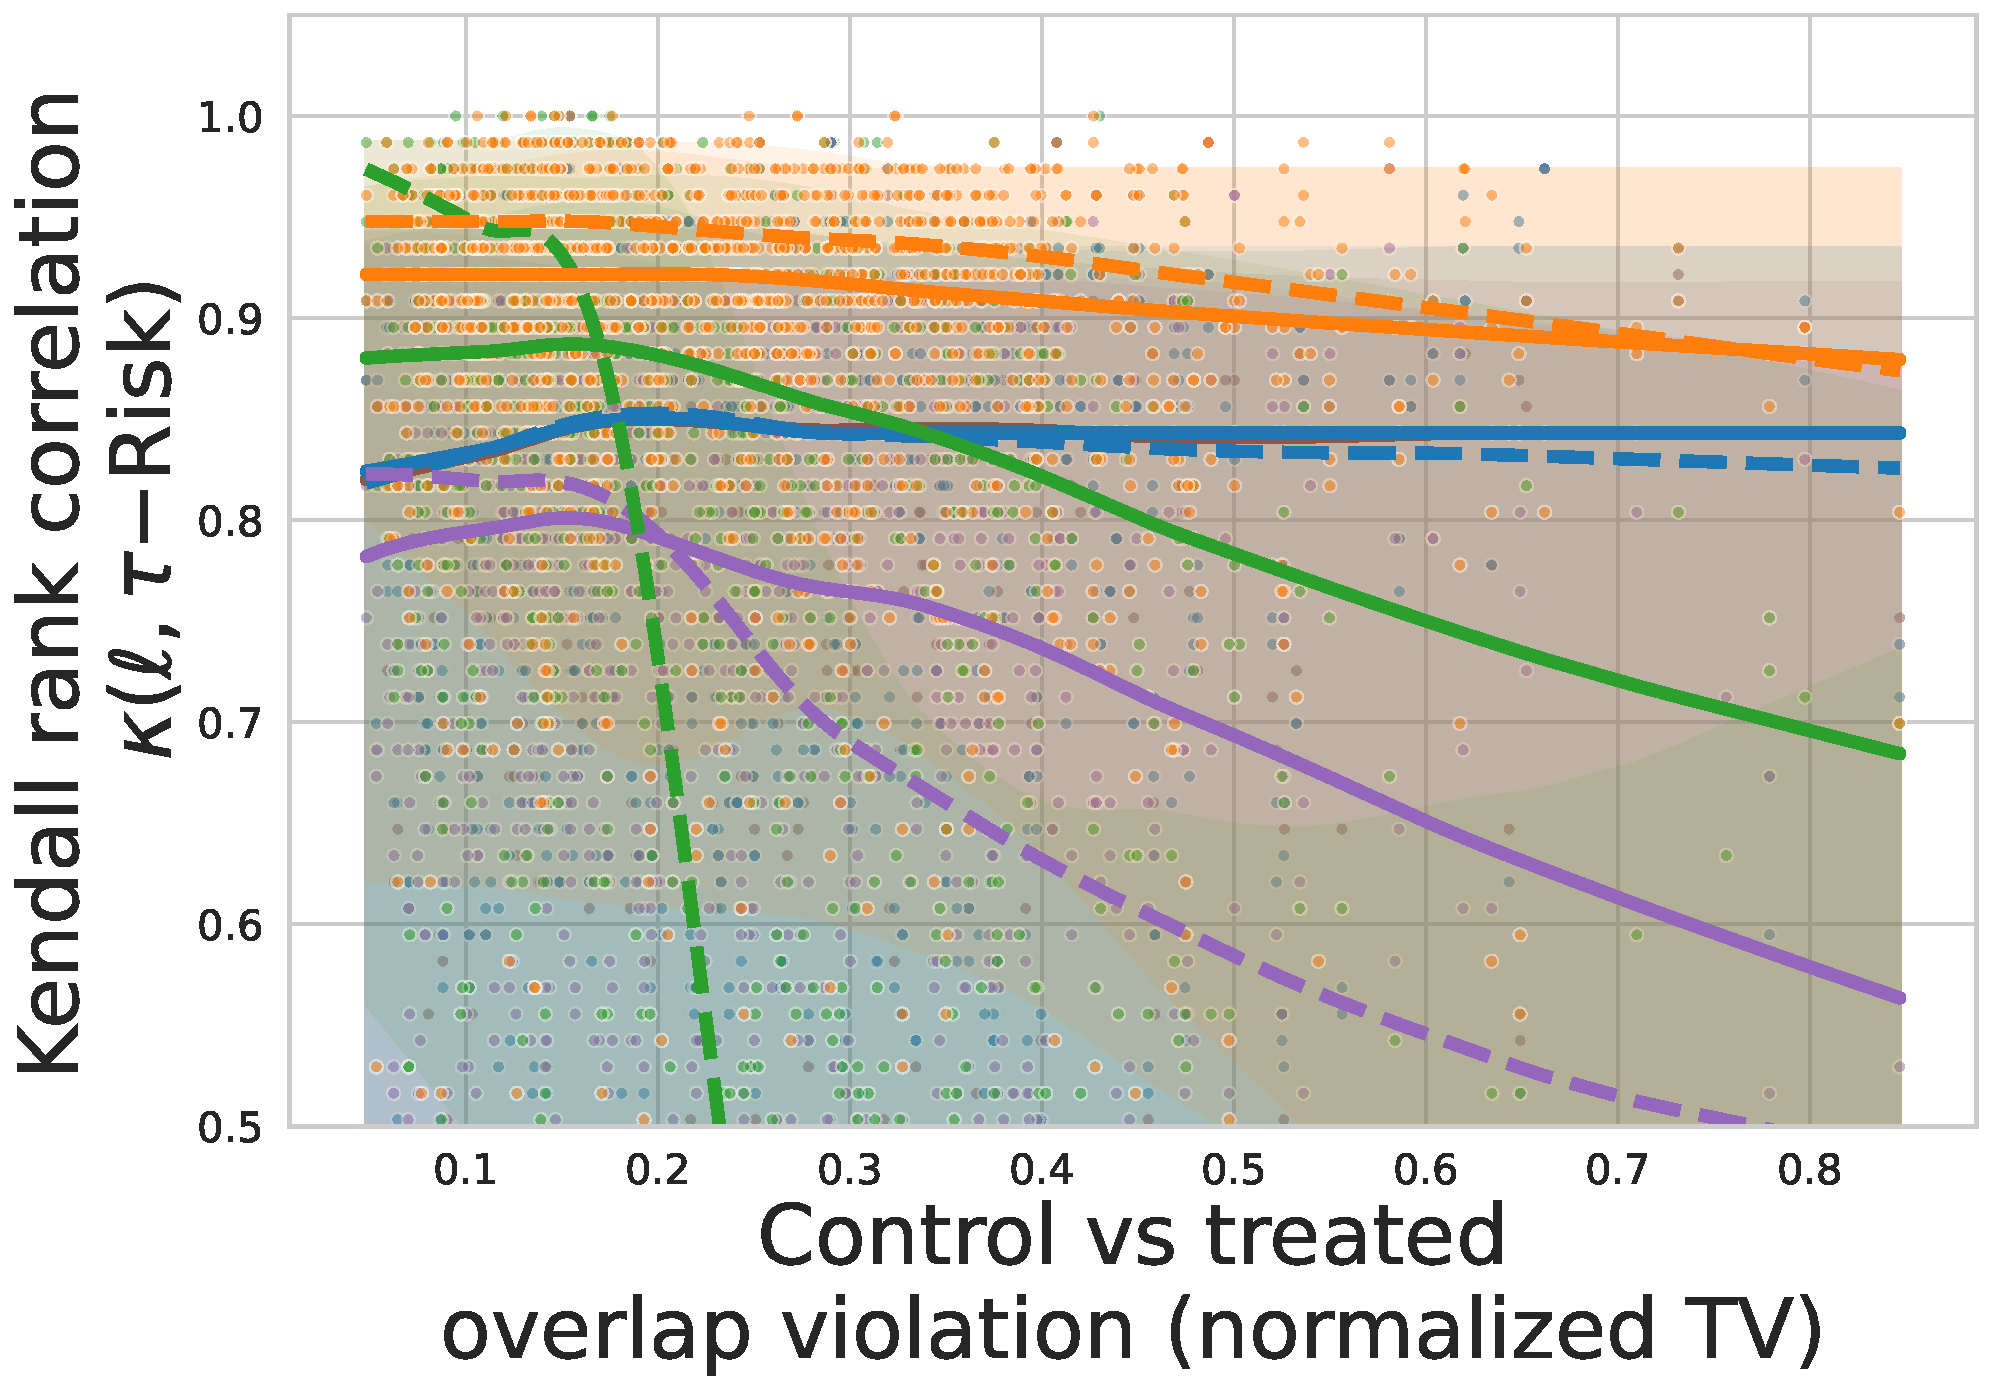
\includegraphics[width=\textwidth]{kendalls_tau_acic_2016__nuisance_non_linear__candidates_hist_gradient_boosting__dgp_1-77__rs_1-10.pdf}
            \label{fig:ranking_agreement_tau_risk_acic_2016}
        \end{subfigure}
        \hfill
        \begin{subfigure}[b]{0.10\textwidth}
            \centering
            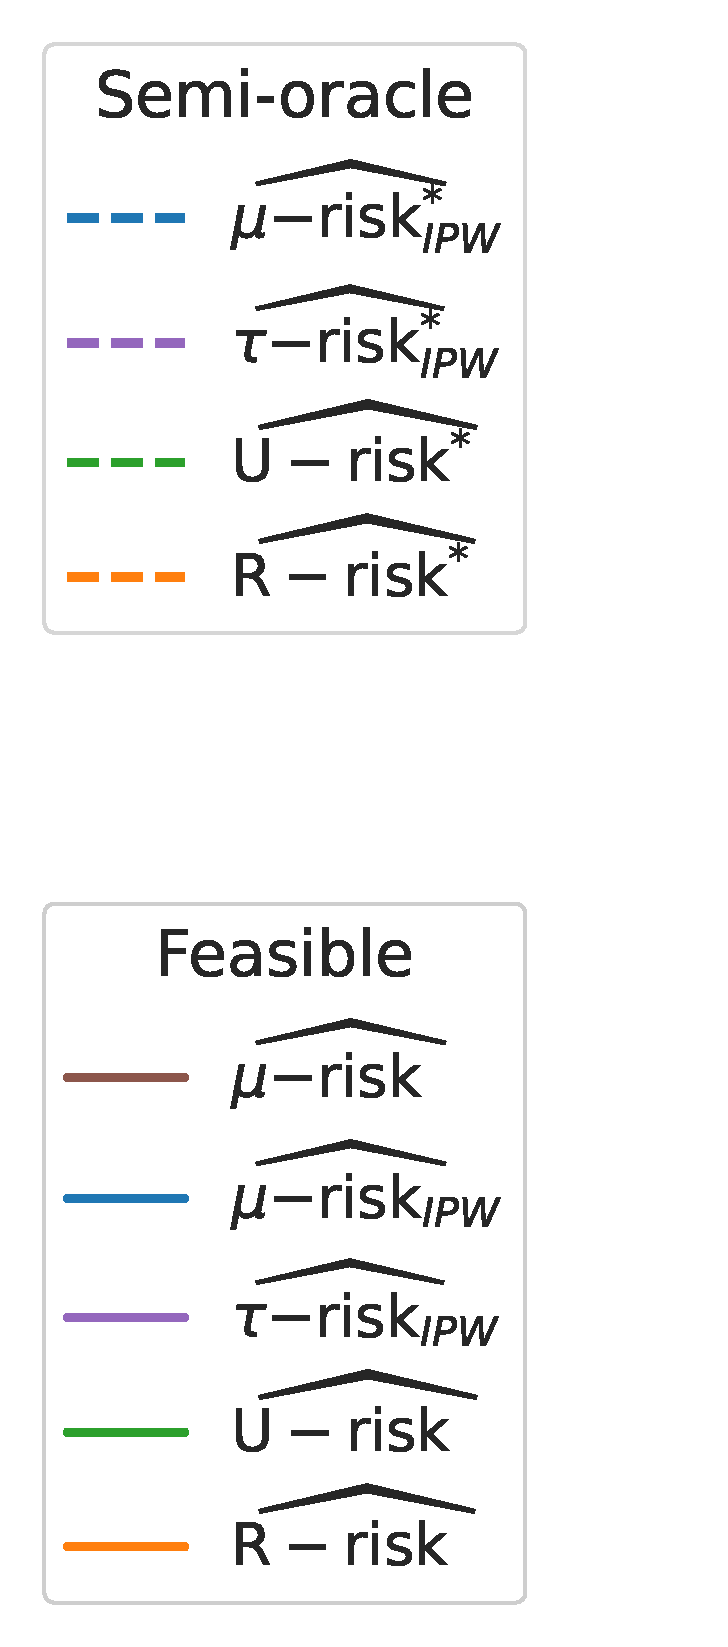
\includegraphics[width=1.5\textwidth]{legend_metrics.pdf}
        \end{subfigure}
        \begin{subfigure}[b]{0.44\textwidth}
            \centering
            \caption{\textbf{ACIC 2018}}
            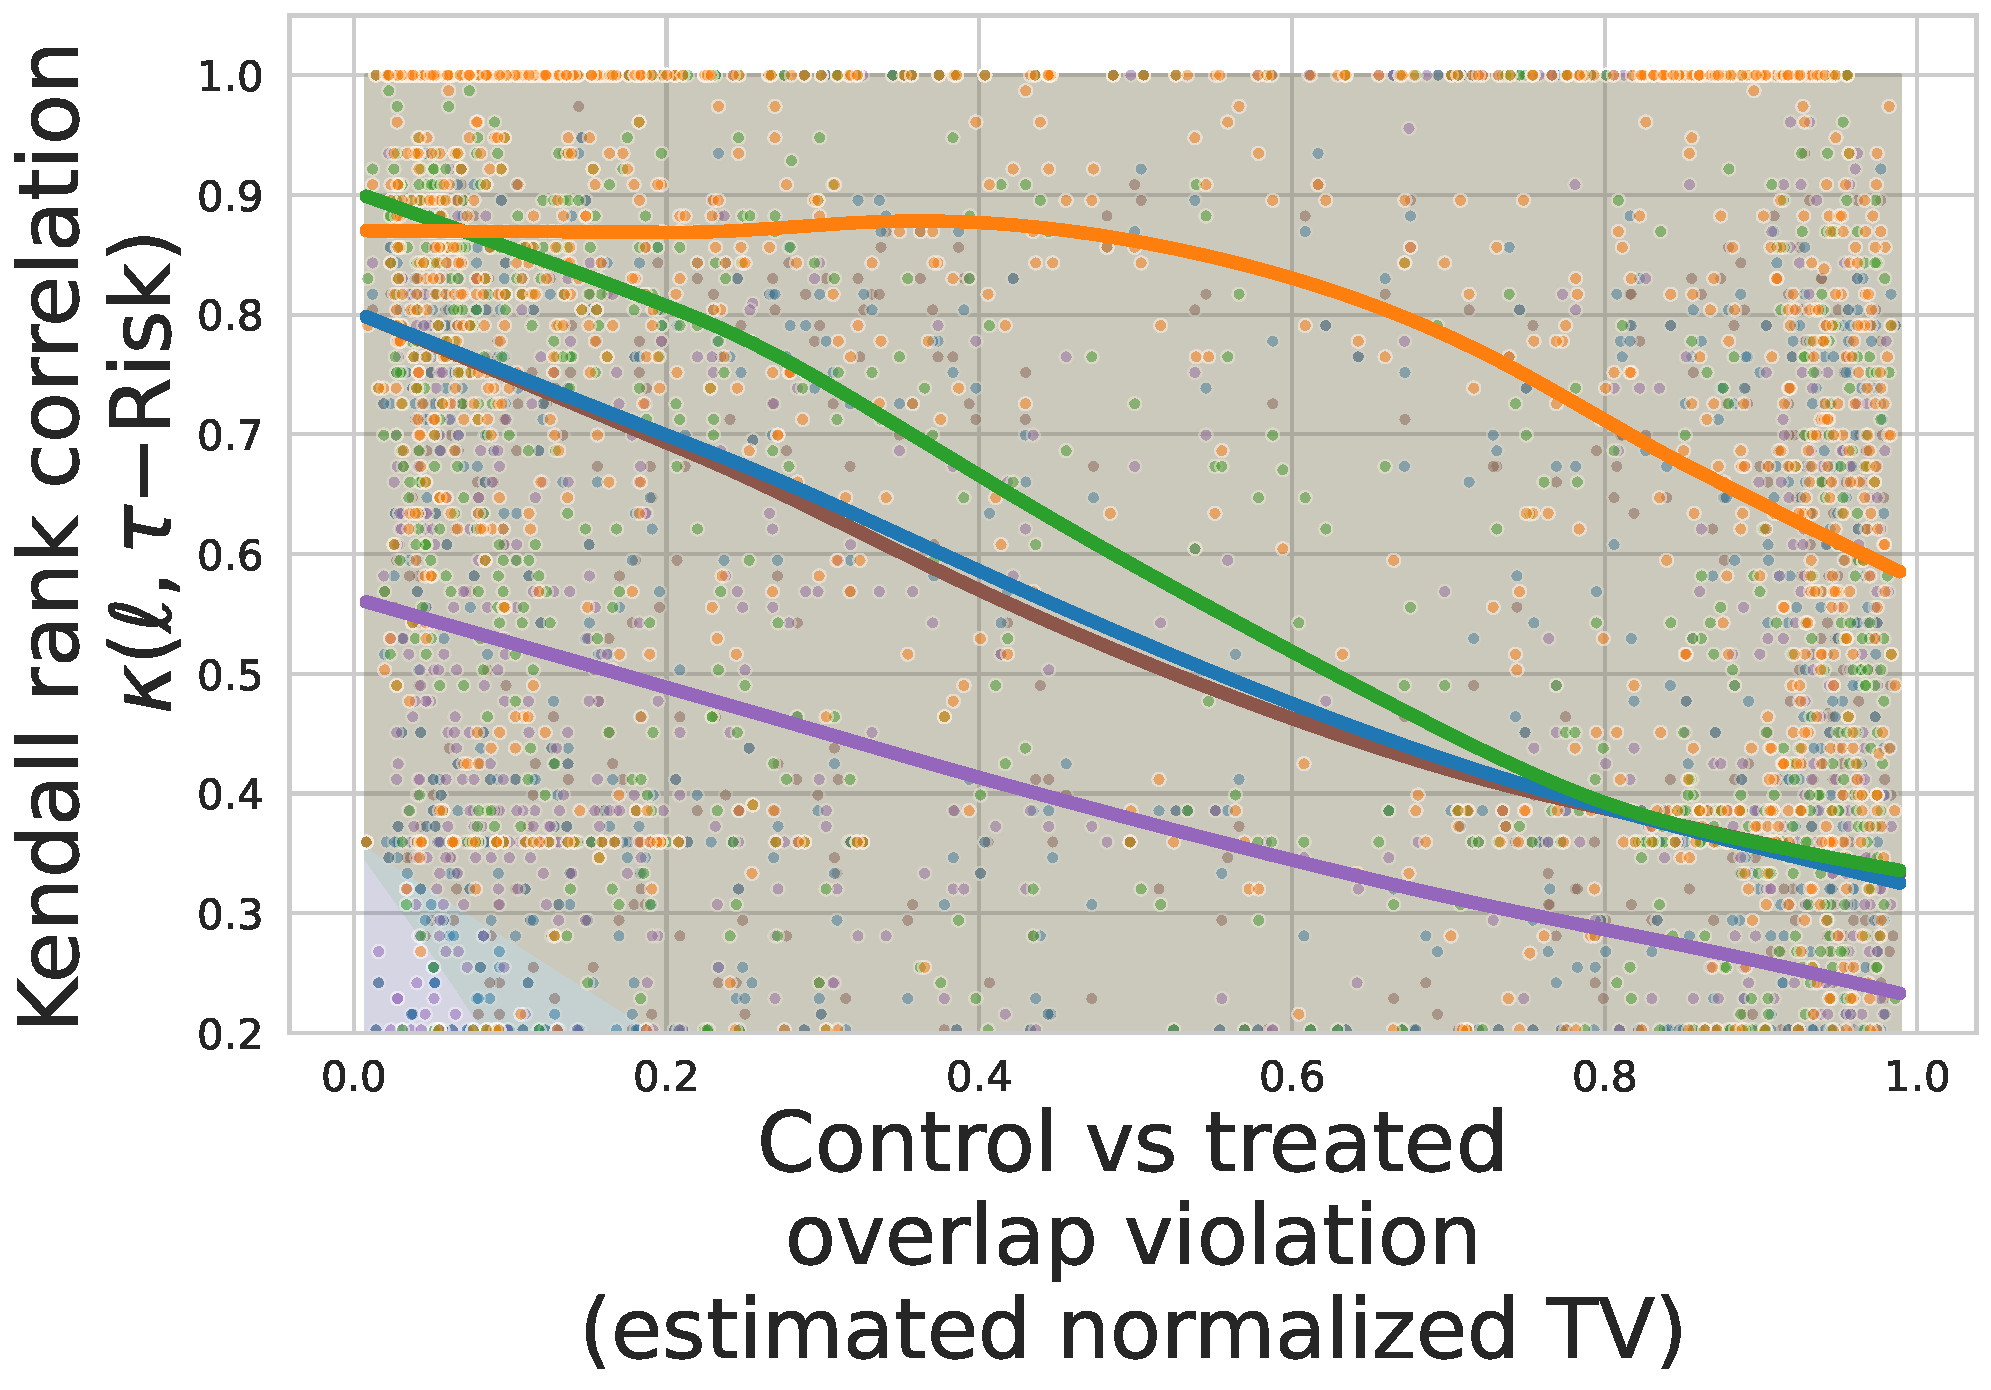
\includegraphics[width=\textwidth]{kendalls_tau_acic_2018__nuisance_stacking__candidates_hist_gradient_boosting__tset_50.pdf}
            \label{fig:ranking_agreement_w_tau_risk_acic_2018}
        \end{subfigure}
        \hfill
        \begin{subfigure}[b]{0.44\textwidth}
            \centering
            \caption{\textbf{TWINS}}
            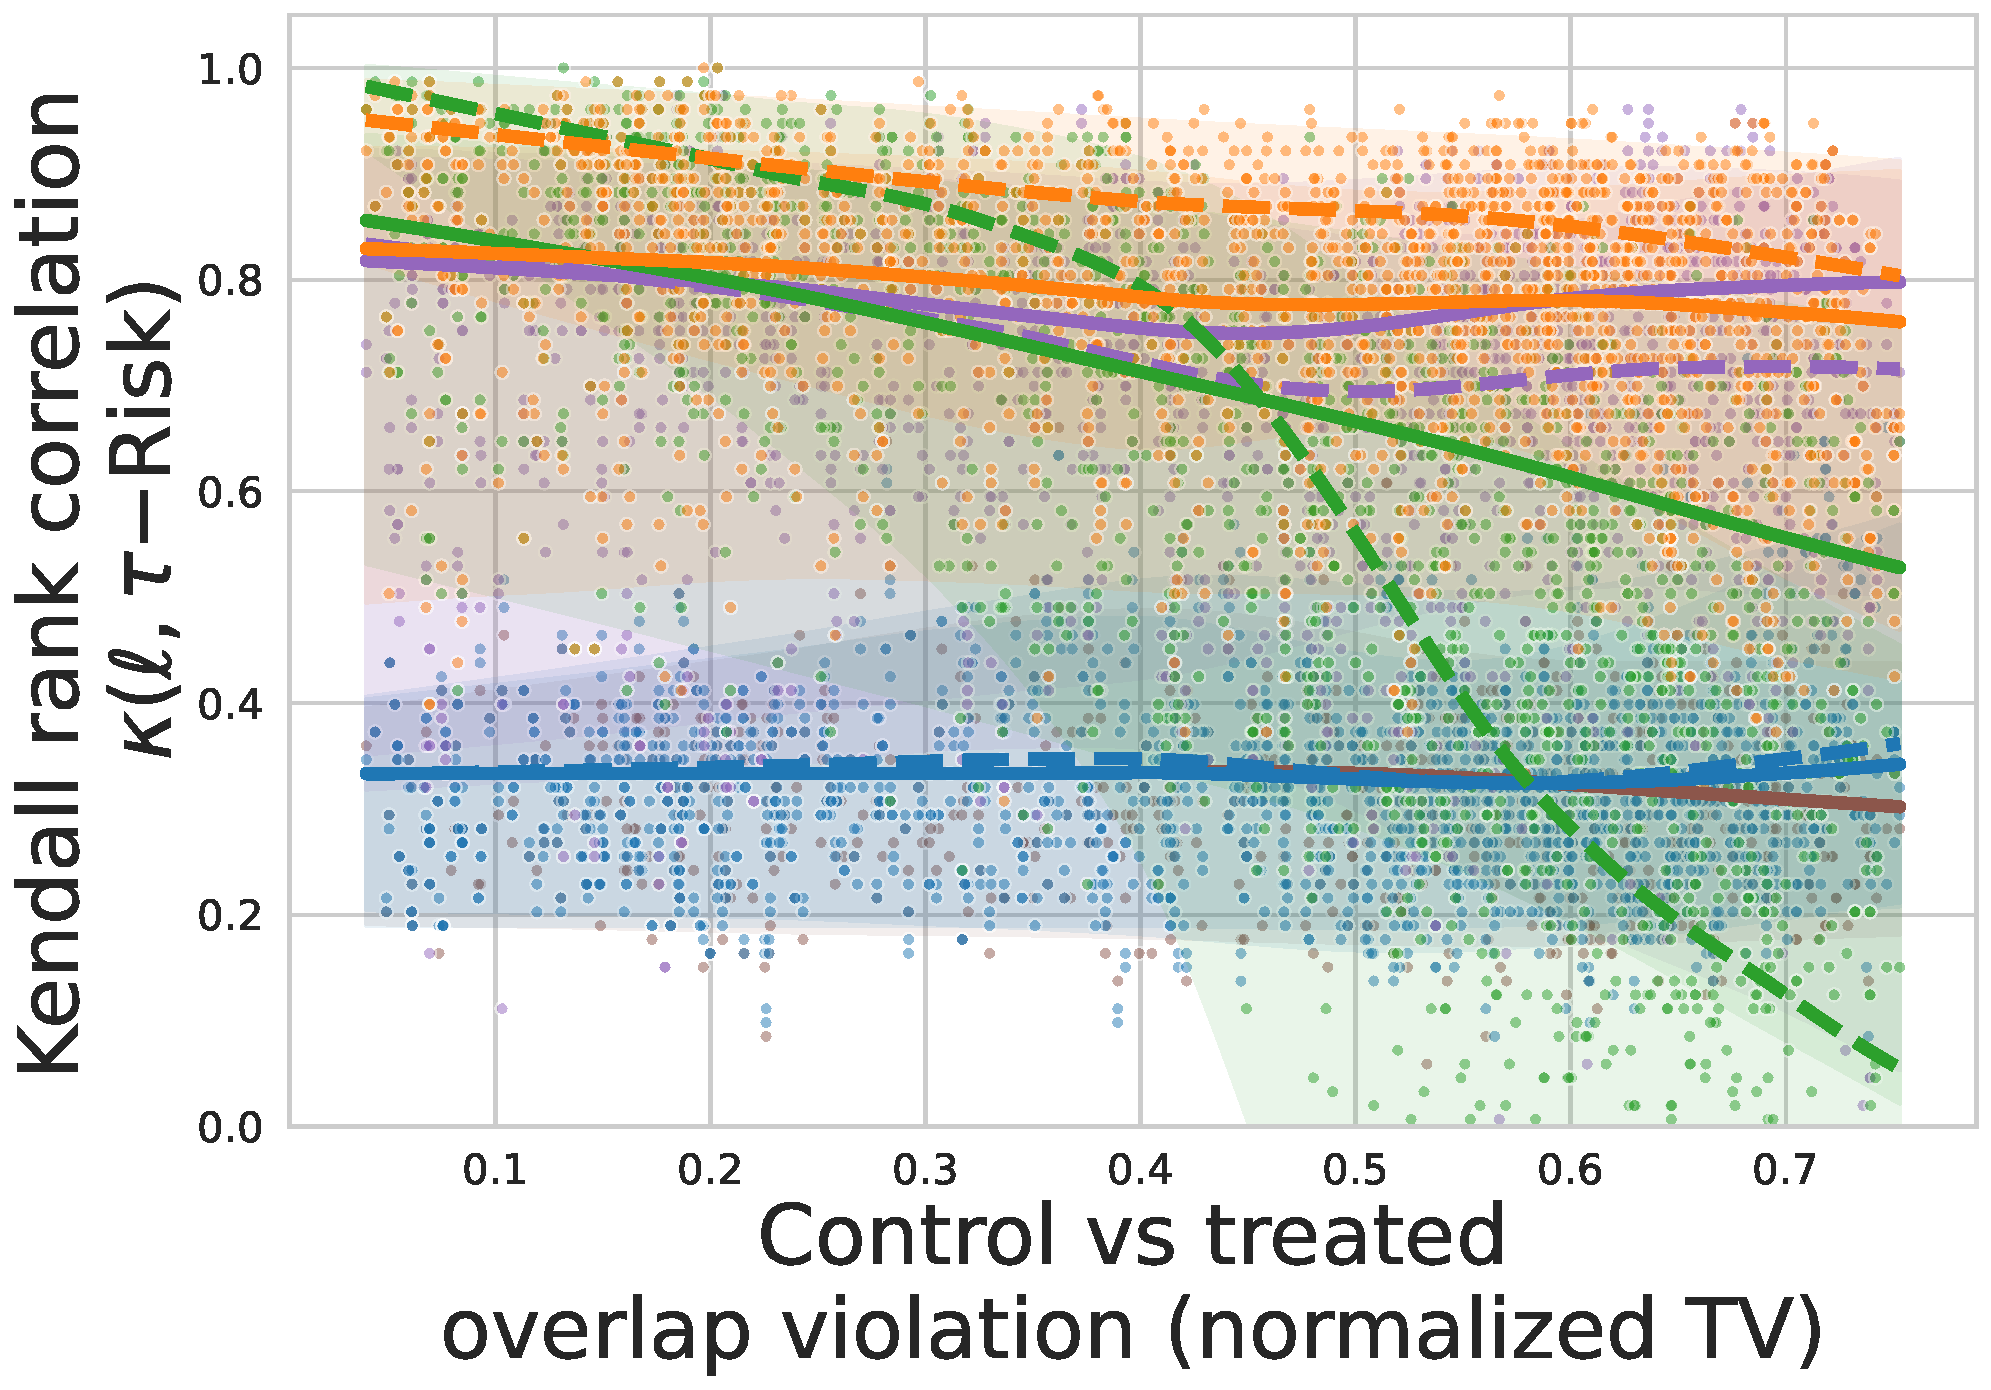
\includegraphics[width=\textwidth]{kendalls_tau_twins__nuisance_stacking__candidates_hist_gradient_boosting__tset_50__overlap_11-296__rs_0-9_noise10.pdf}
            \label{fig:ranking_agreement_tau_risk_twins}
        \end{subfigure}
        \hfill
        \begin{subfigure}[b]{0.10\textwidth}
            ~
        \end{subfigure}
        % \begin{subfigure}[b]{\textwidth}
        %   \centering
        %   \includegraphics[width=0.5\textwidth]{legend_metrics_horizontal.pdf}
        % \end{subfigure}
        \caption{Agreement with $\tau\text{-risk}$ ranking of methods function
            of overlap violation. The lines represent medians, estimated with a
            lowess. The transparent
            bands denote the 5\% and 95\% confidence intervals.}\label{apd:fig:all_datasets_tau_risk_ranking_agreement}
    \end{figure}



    \paragraph{Figure \ref{apd:all_datasets_normalized_bias_tau_risk_to_best_method}
        - Results measured as distance to the oracle tau-risk}

    To see practical gain in term of $\tau\text{-risk}$, we plot the results as the
    normalized distance between the estimator selected by the oracle
    $\tau\text{-risk}$ and the estimator selected by each causal metric.

    Then, $\widehat{R\text{-risk}}^*$ is more efficient than all other metrics. The
    gain are substantial for every datasets.

    \begin{figure}
        \centering
        \begin{subfigure}[b]{0.44\textwidth}
            \centering
            \caption{\textbf{Caussim}}
            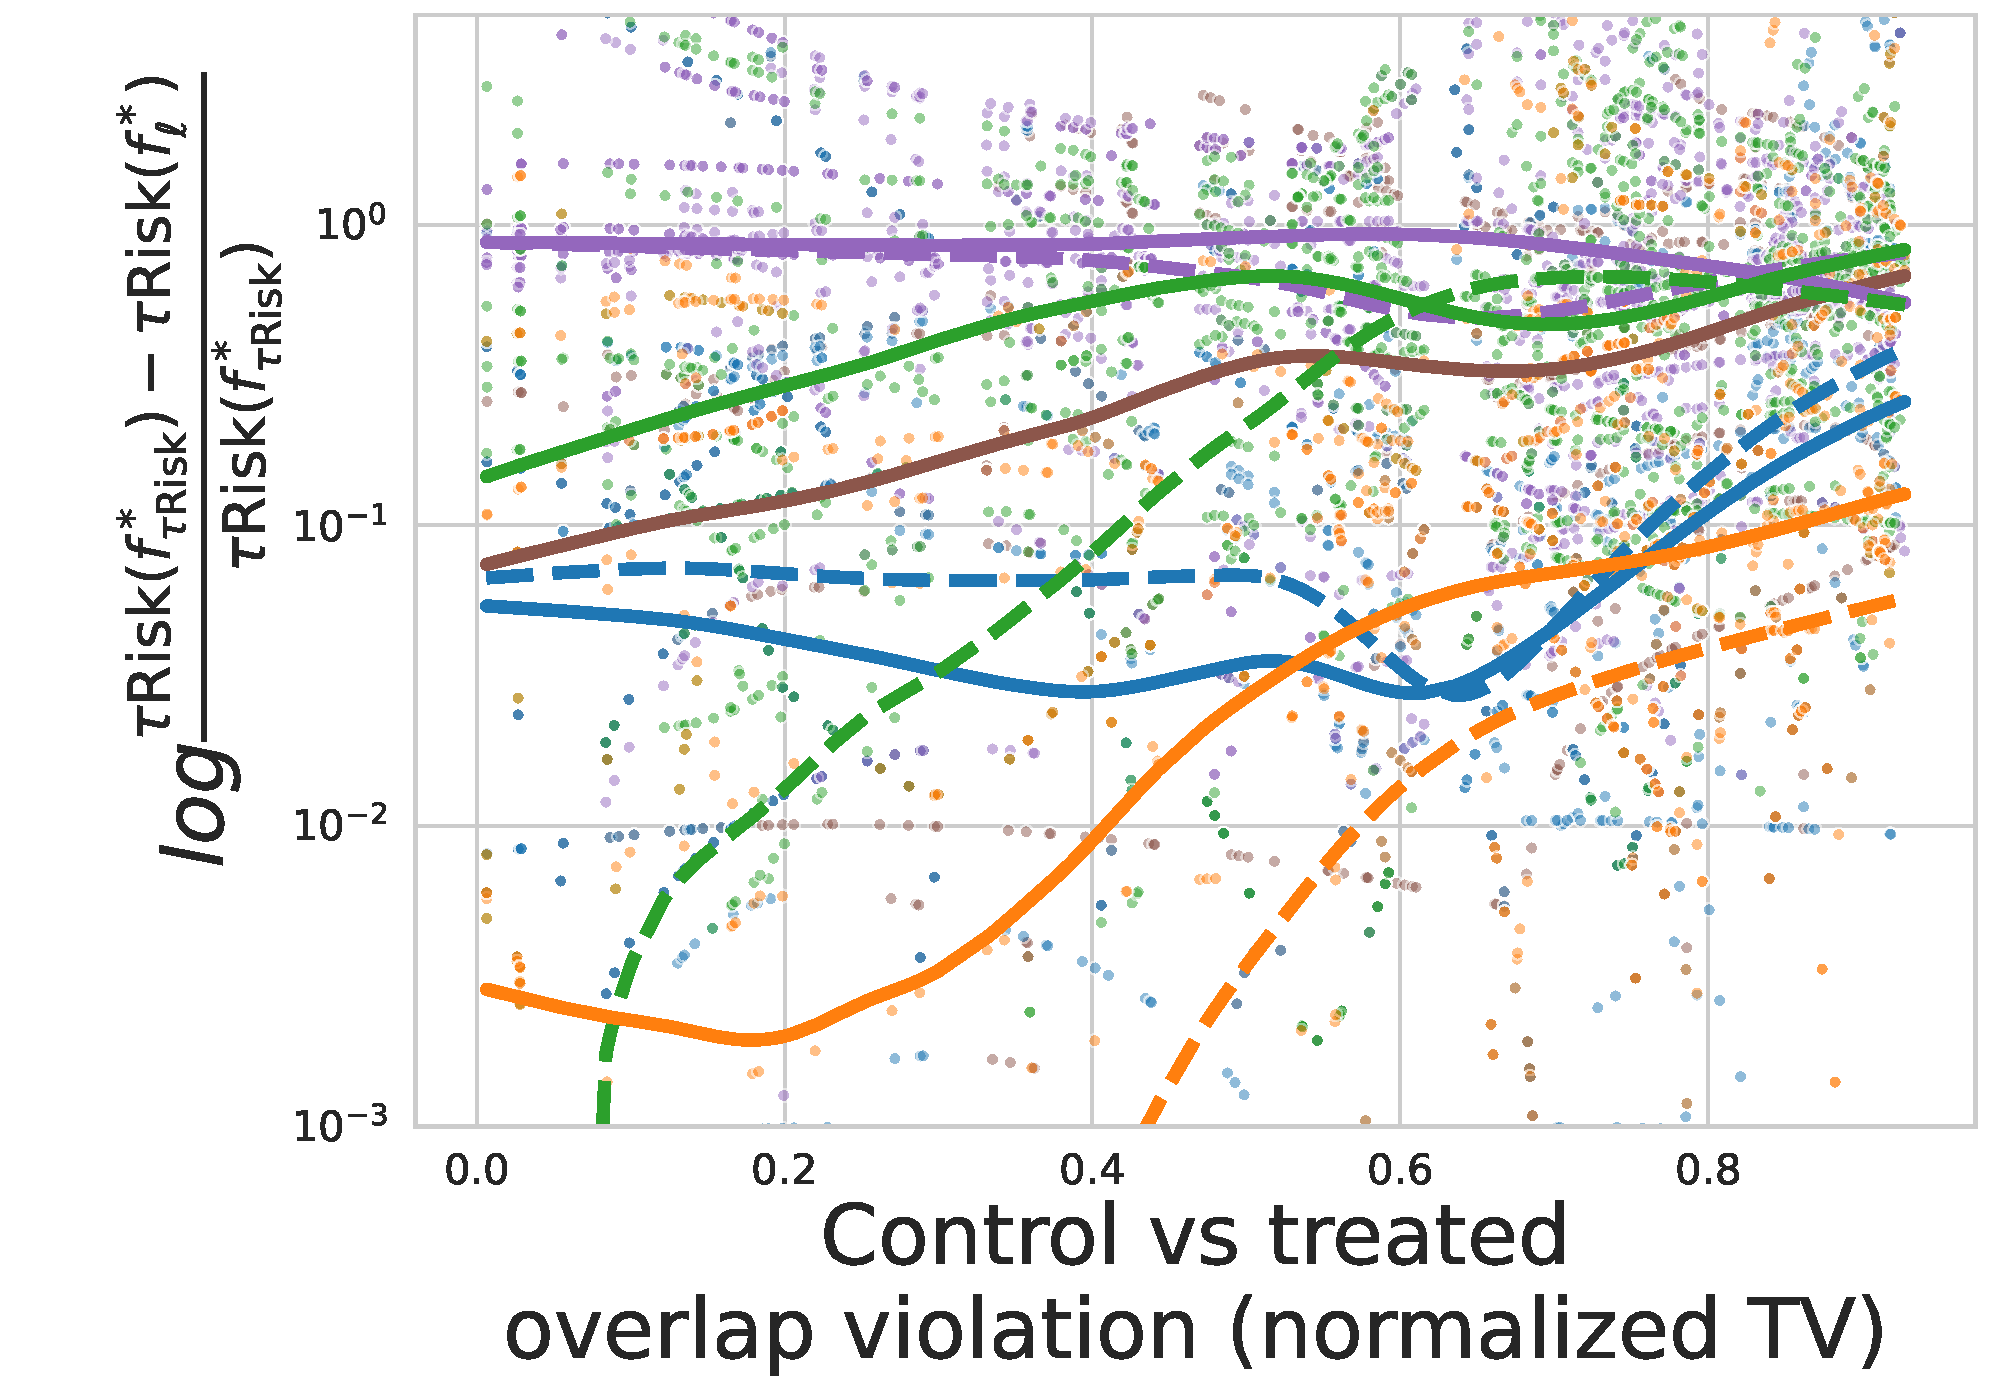
\includegraphics[width=\textwidth]{normalized_bias_tau_risk_to_best_method_caussim__nuisance_non_linear__candidates_ridge__overlap_01-247.pdf}
            \label{fig:normalized_bias_tau_risk_to_best_method_caussim}
        \end{subfigure}
        \hfill
        \begin{subfigure}[b]{0.44\textwidth}
            \centering
            \caption{\textbf{ACIC 2016}}
            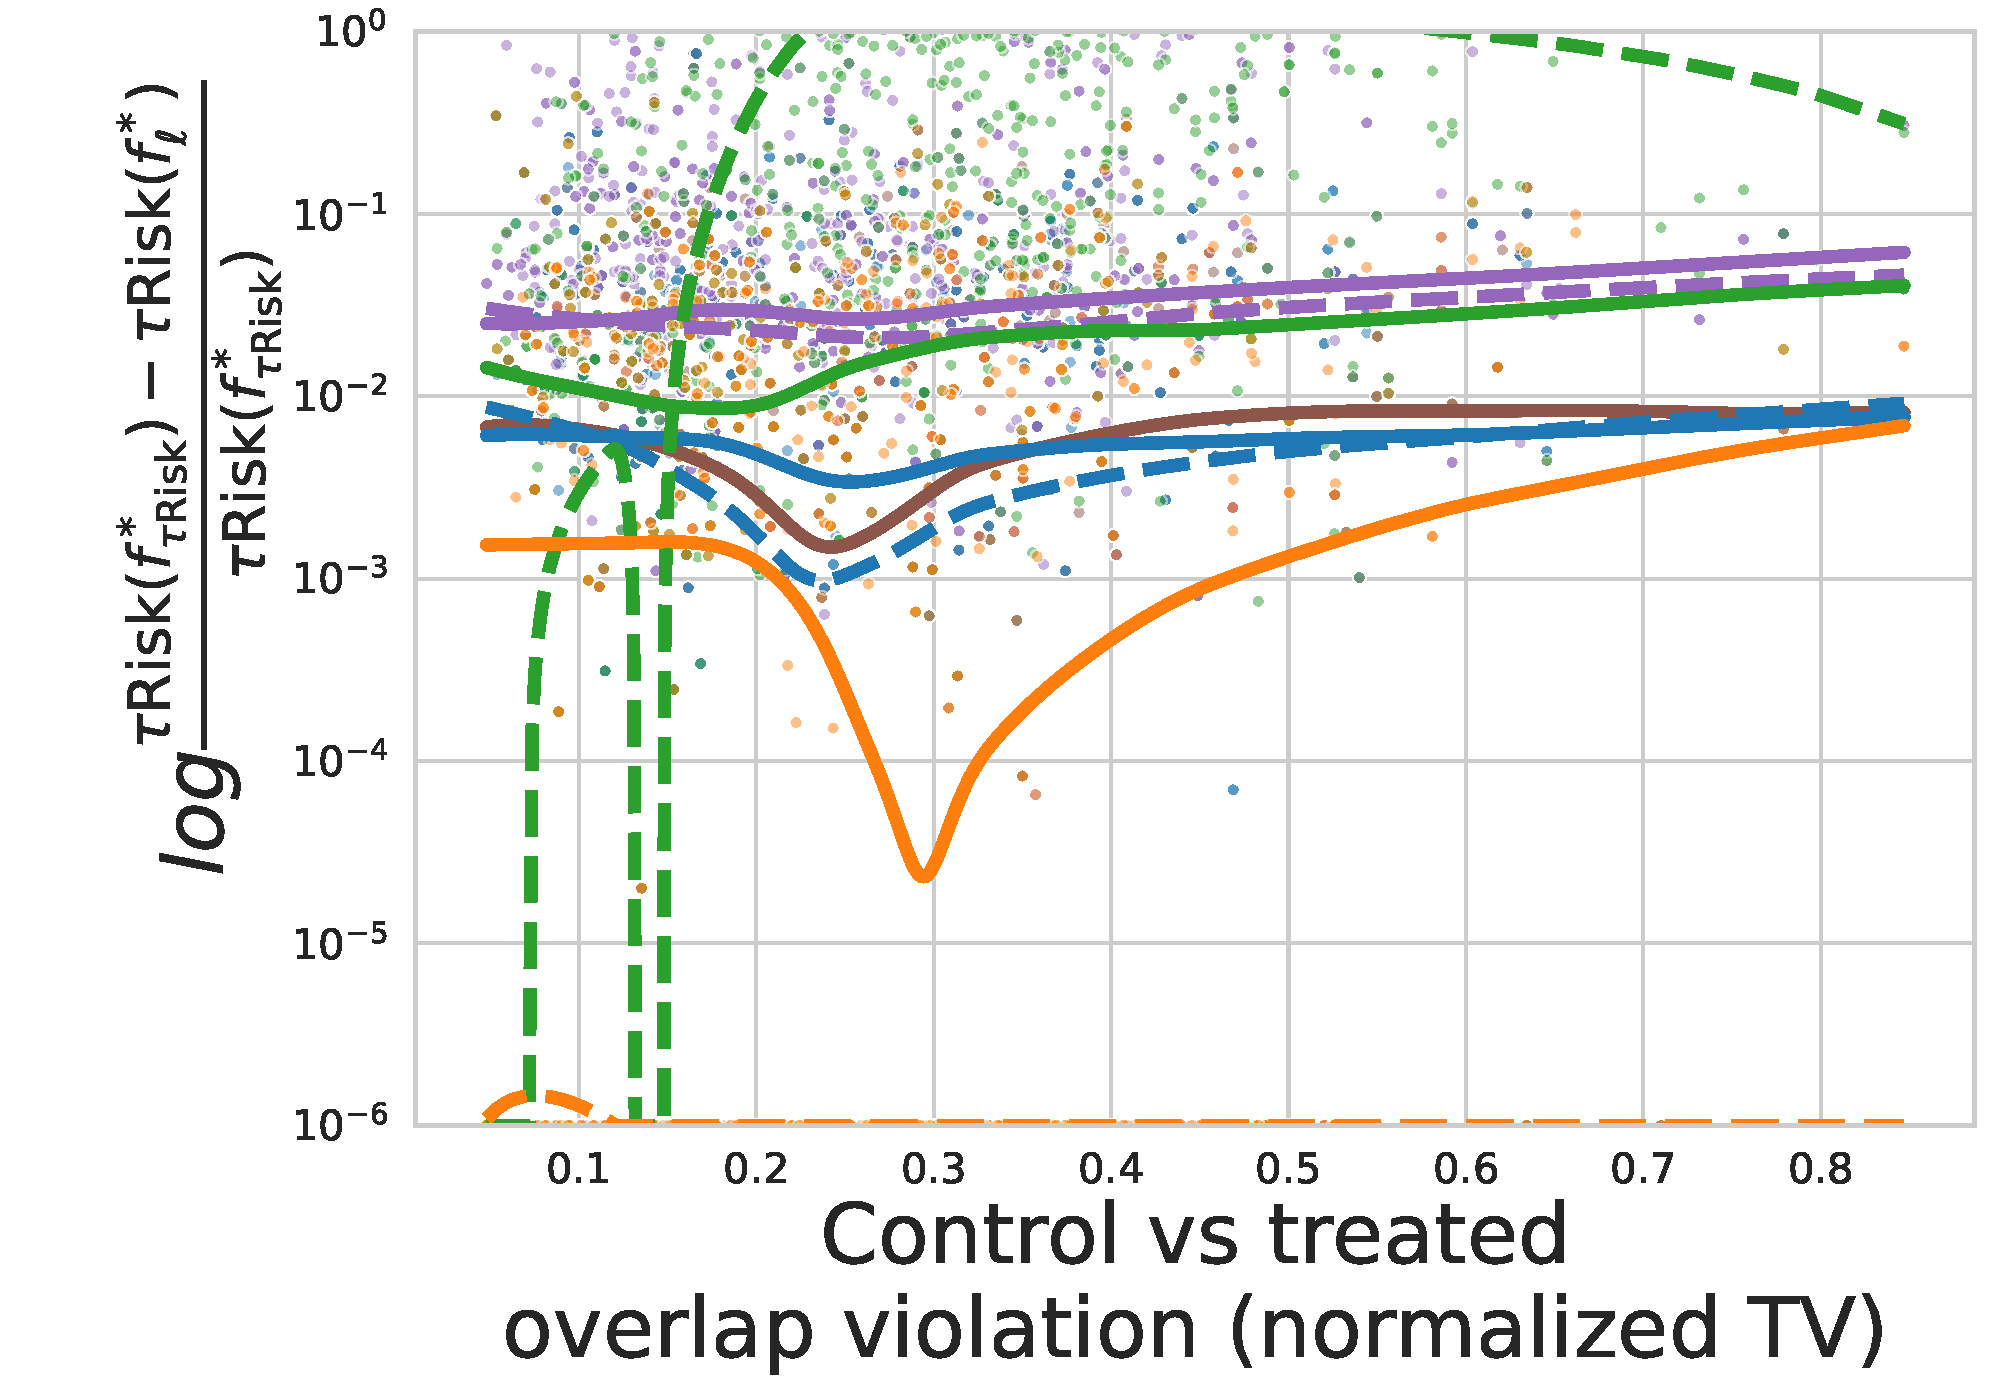
\includegraphics[width=\textwidth]{normalized_bias_tau_risk_to_best_method_acic_2016__nuisance_non_linear__candidates_hist_gradient_boosting__dgp_1-77__rs_1-10.pdf}
            \label{fig:normalized_bias_tau_risk_to_best_method_acic_2016}
        \end{subfigure}
        \hfill
        \begin{subfigure}[b]{0.10\textwidth}
            \centering
            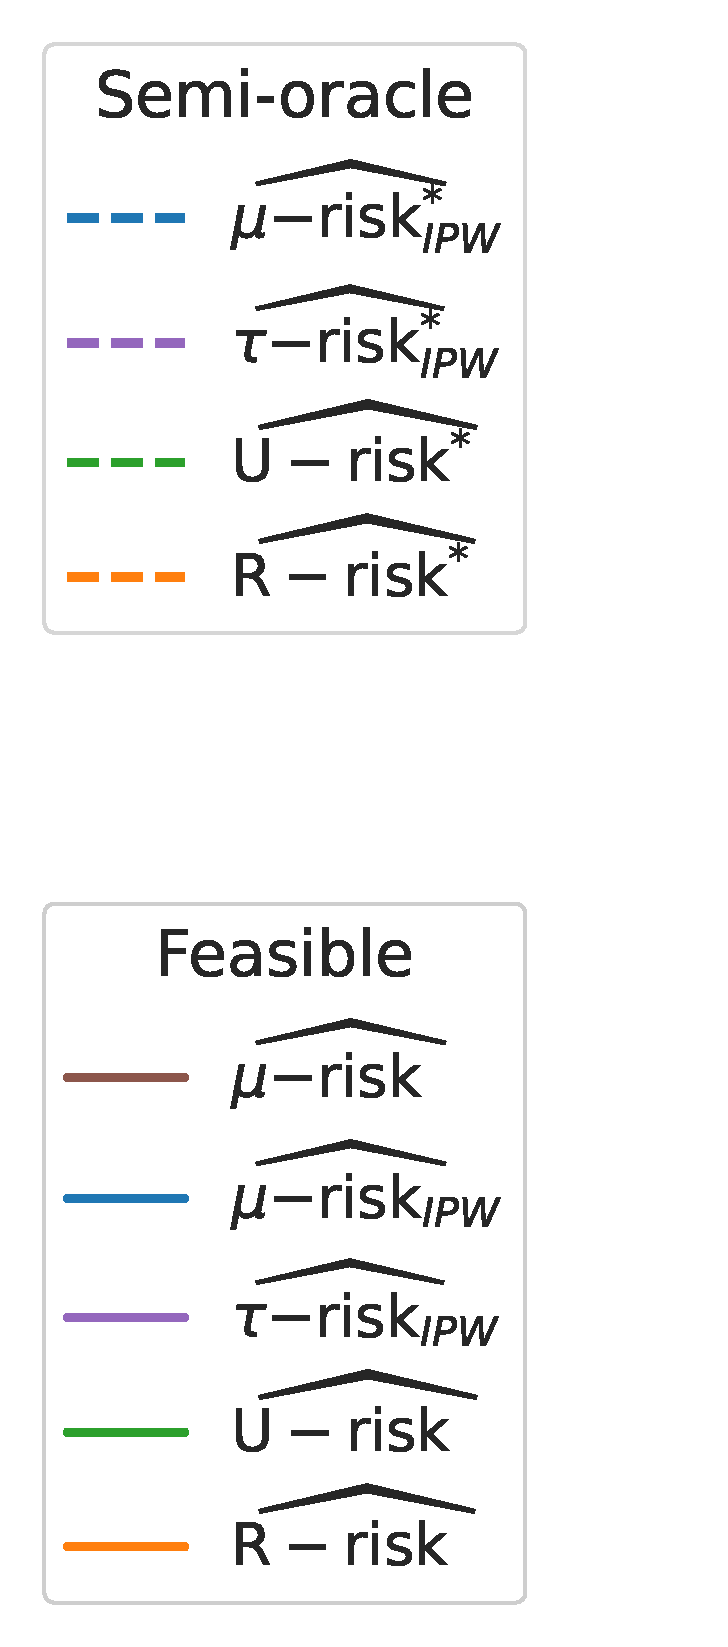
\includegraphics[width=1.5\textwidth]{legend_metrics.pdf}
        \end{subfigure}
        \begin{subfigure}[b]{0.44\textwidth}
            \centering
            \caption{\textbf{ACIC 2018}}
            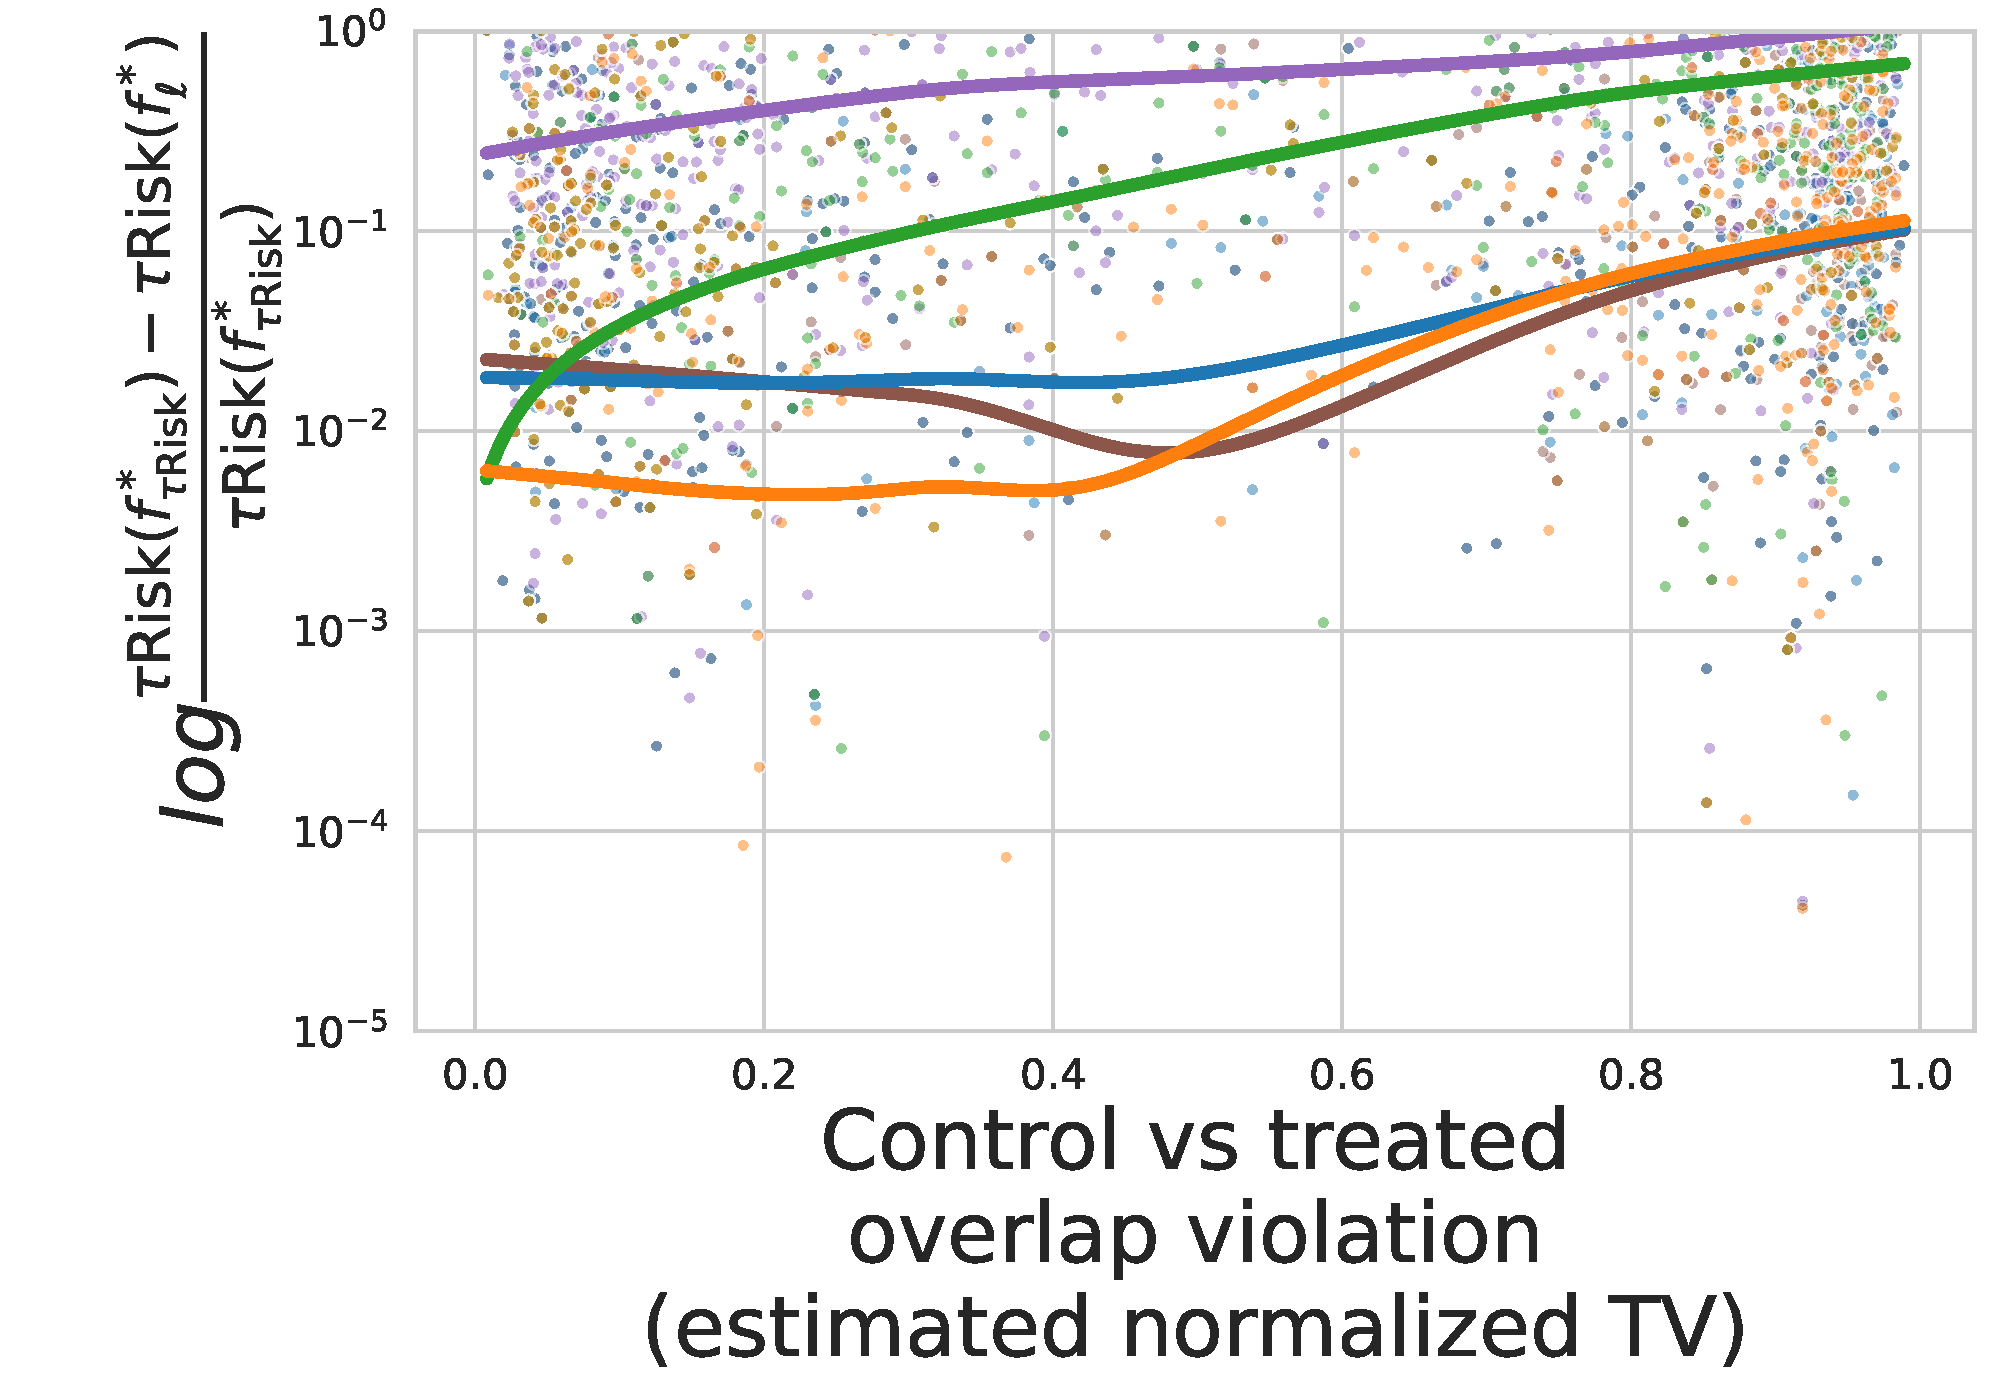
\includegraphics[width=\textwidth]{normalized_bias_tau_risk_to_best_method_acic_2018__nuisance_stacking__candidates_hist_gradient_boosting__tset_50.pdf}
            \label{fig:normalized_bias_tau_risk_to_best_method_acic_2018}
        \end{subfigure}
        \hfill
        \begin{subfigure}[b]{0.44\textwidth}
            \centering
            \caption{\textbf{TWINS}}
            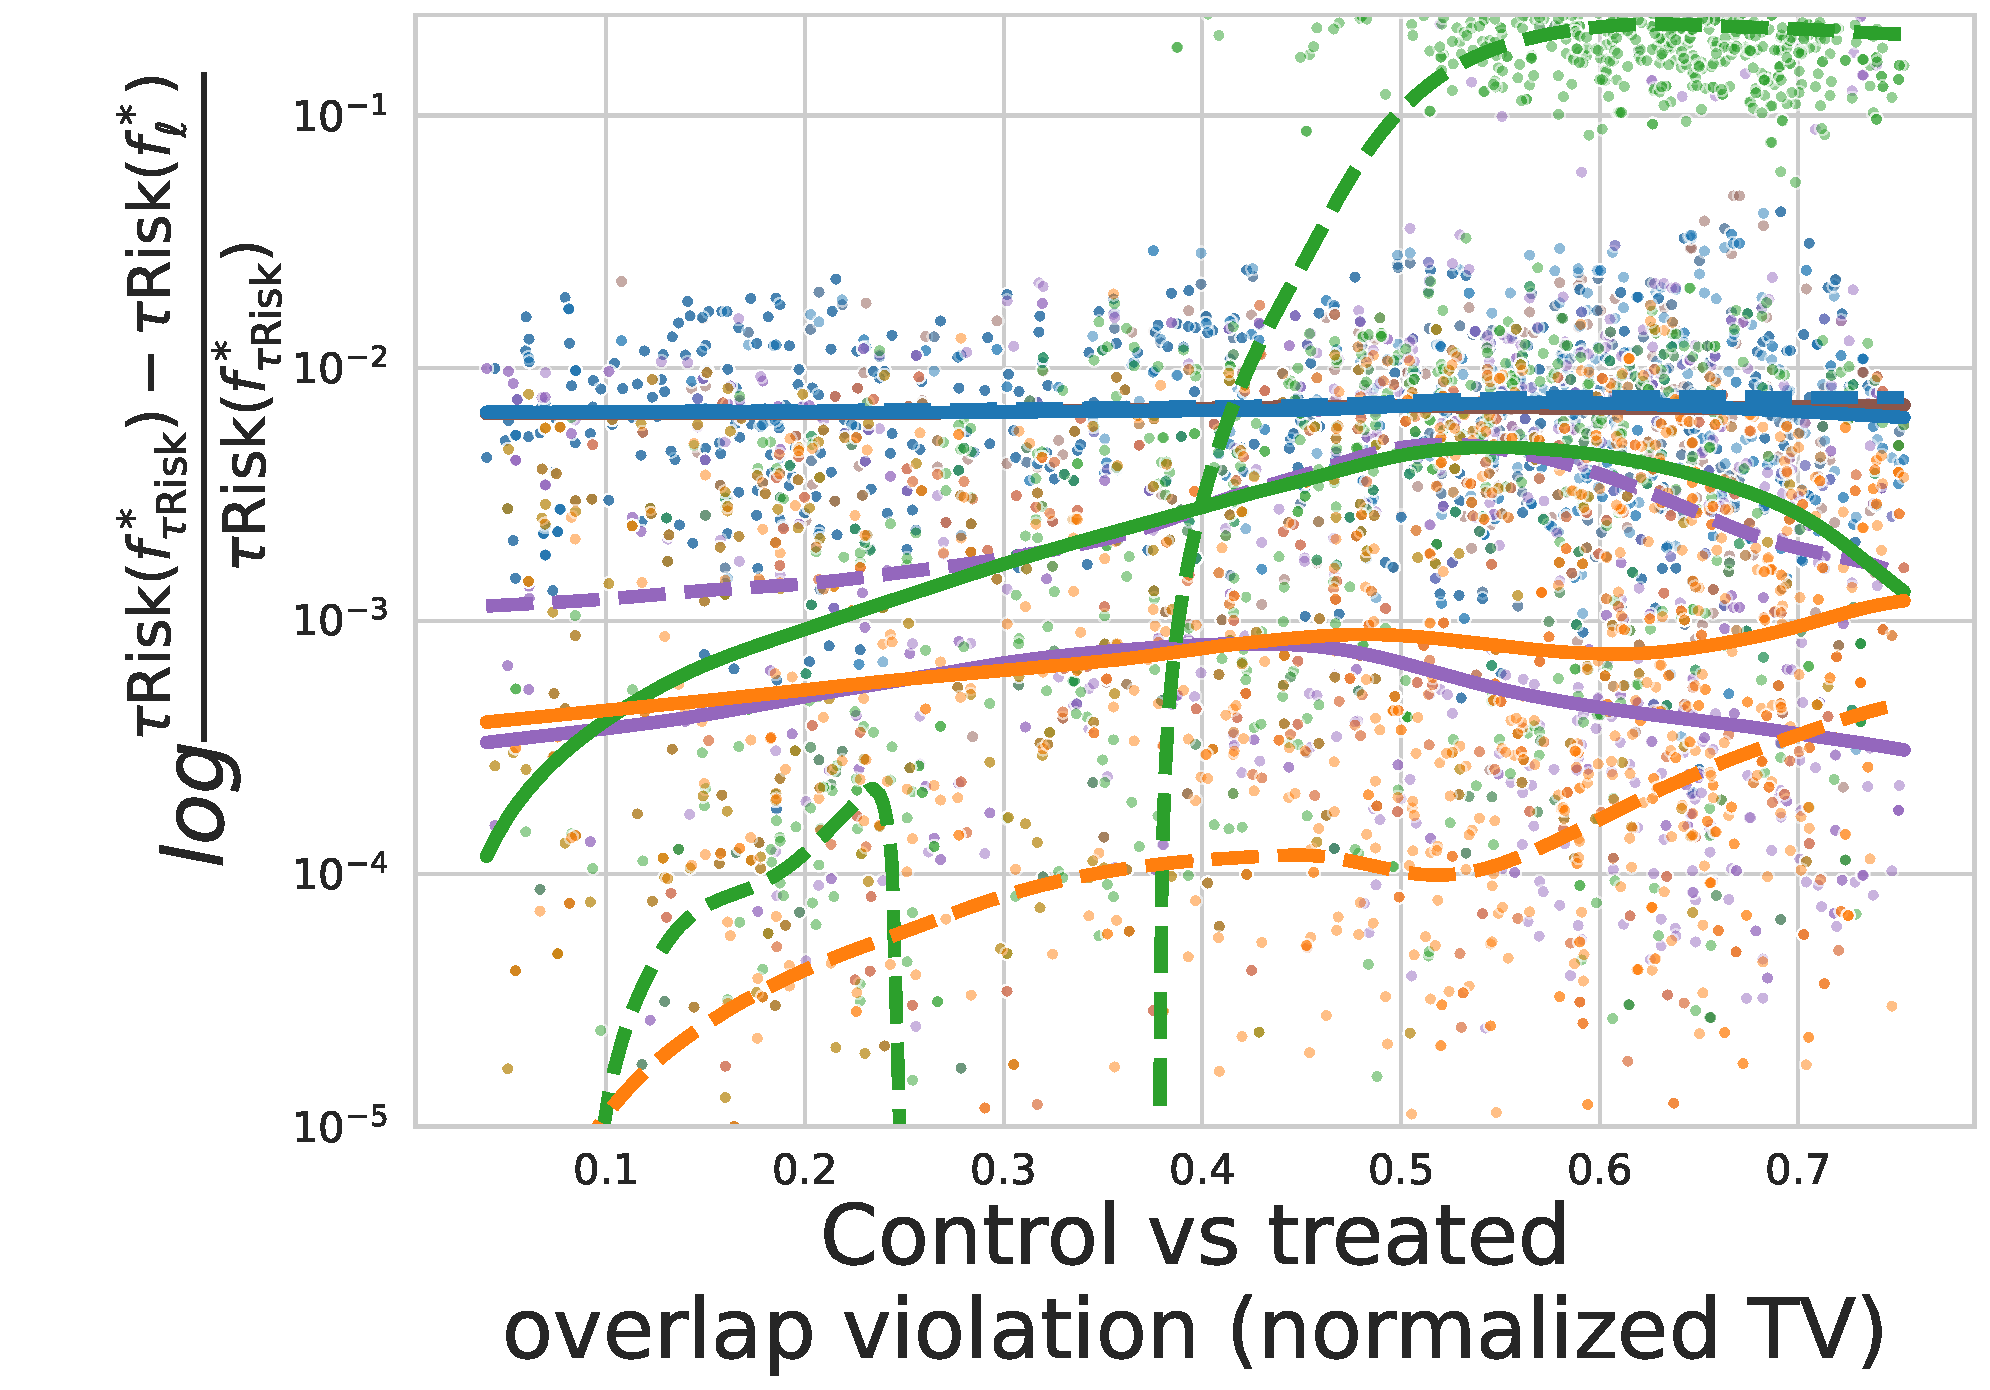
\includegraphics[width=\textwidth]{normalized_bias_tau_risk_to_best_method_twins__nuisance_stacking__candidates_hist_gradient_boosting__tset_50__overlap_11-296__rs_0-9_noise10.pdf}
            \label{fig:normalized_bias_tau_risk_to_best_method_twins}
        \end{subfigure}
        \hfill
        \begin{subfigure}[b]{0.10\textwidth}
            ~
        \end{subfigure}
        \caption{Metric performances by normalized tau-risk distance to the best
            method selected with $\tau\text{-risk}$. All nuisances are learned with the
            same estimator stacking gradient boosting and ridge regression. Doted and
            plain lines corresponds to 60\% lowess quantile estimates. This choice of
            quantile allows to see better the oracle metrics lines for which outliers with a value
            of 0 distord the curves.}
        \label
        {apd:all_datasets_normalized_bias_tau_risk_to_best_method}
    \end{figure}



    \paragraph{Figure \ref{apd:fig:procedures_comparison_all_metrics} - Stacked models for the nuisances is more efficient}
    For each metrics the benefit of
    using a stacked model of linear and boosting estimators for nuisances compared
    to a linear model. The evaluation measure is Kendall's tau relative to the
    oracle $R\text{-risk}^{\star}$ to have a stable reference between exepriments.
    Thus, we do not include in this analysis the ACIC 2018 dataset since
    $R\text{-risk}^{\star}$ is not available due to the lack of the true propensity
    score.

    \begin{figure}
        \begin{subfigure}[b]{0.9\textwidth}
            %\centering
            \caption{\textbf{Caussim}}
            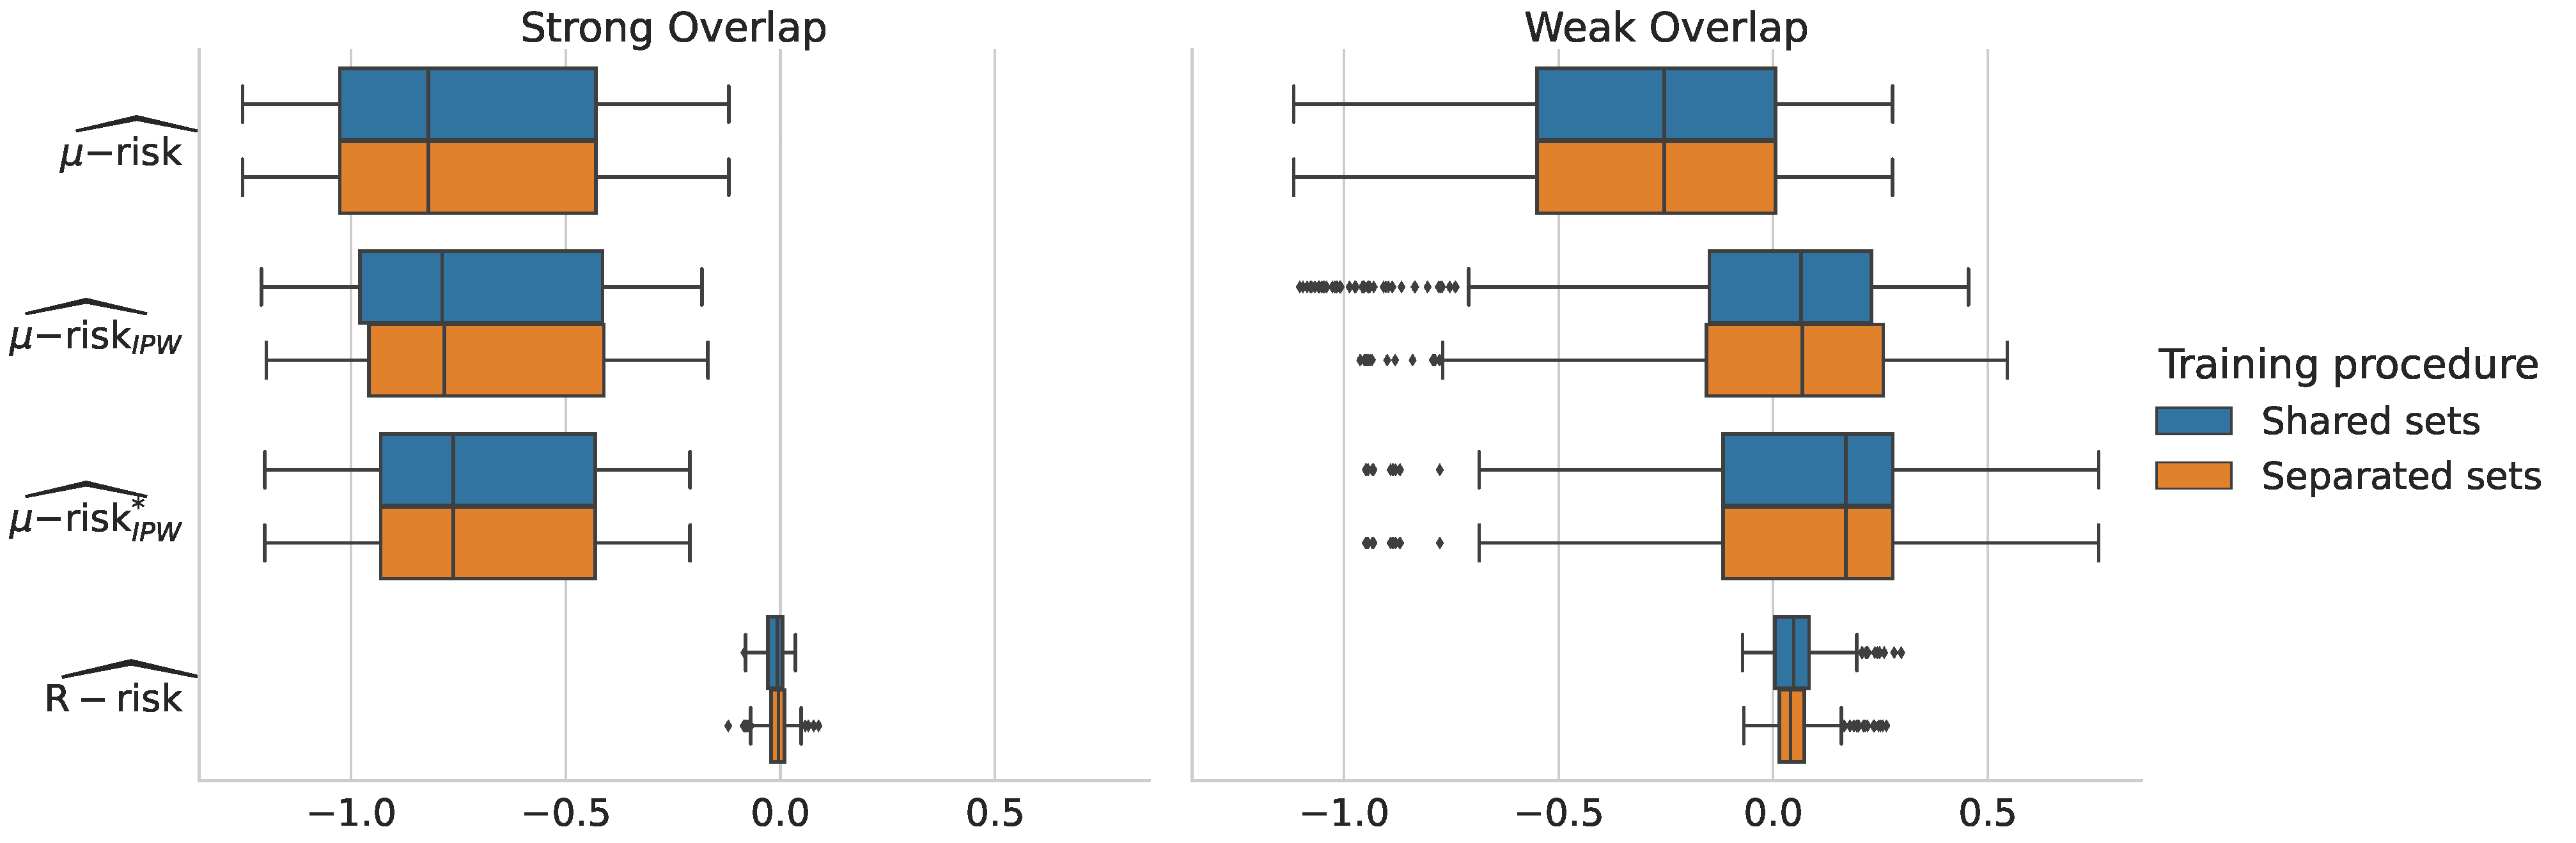
\includegraphics[width=1.15\textwidth]{_3_procedure_Caussim_N5000__ref_metric_oracle_r_risk_training_procedure.pdf}
            \label{fig:experiments:procedures_comparison:caussim}
        \end{subfigure}
        \hfill
        \begin{subfigure}[b]{0.9\textwidth}
            \centering
            \caption{\textbf{ACIC 2016}}
            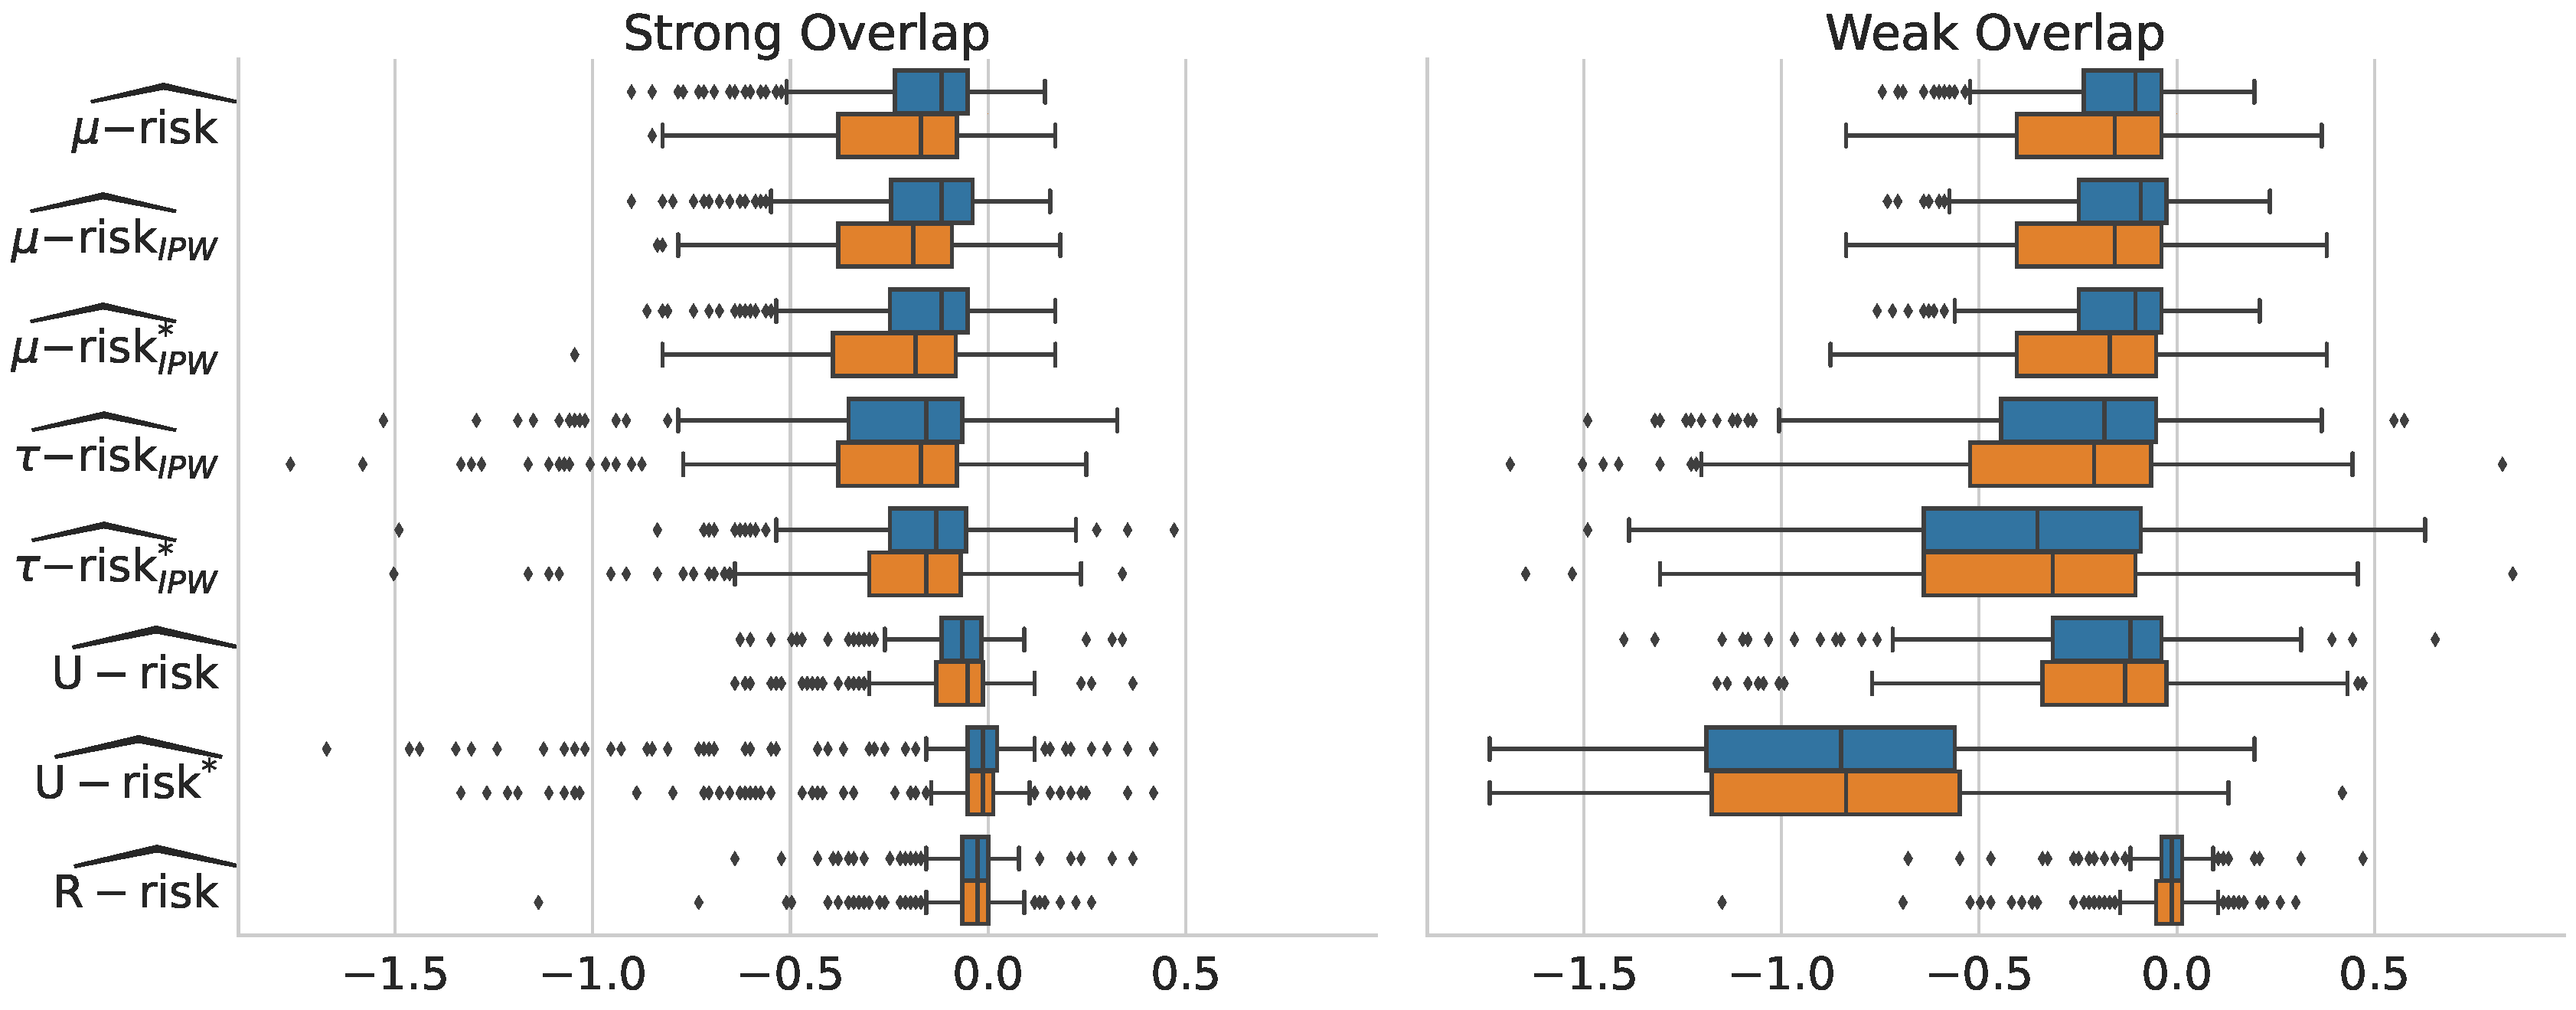
\includegraphics[width=1\textwidth]{_3_procedure_ACIC2016_N4802__ref_metric_oracle_r_risk_training_procedure.pdf}
            \label{fig:experiments:procedures_comparison:acic_2016}
        \end{subfigure}
        \hfill
        \begin{subfigure}[b]{0.9\textwidth}
            \centering
            \caption{\textbf{Twins}}
            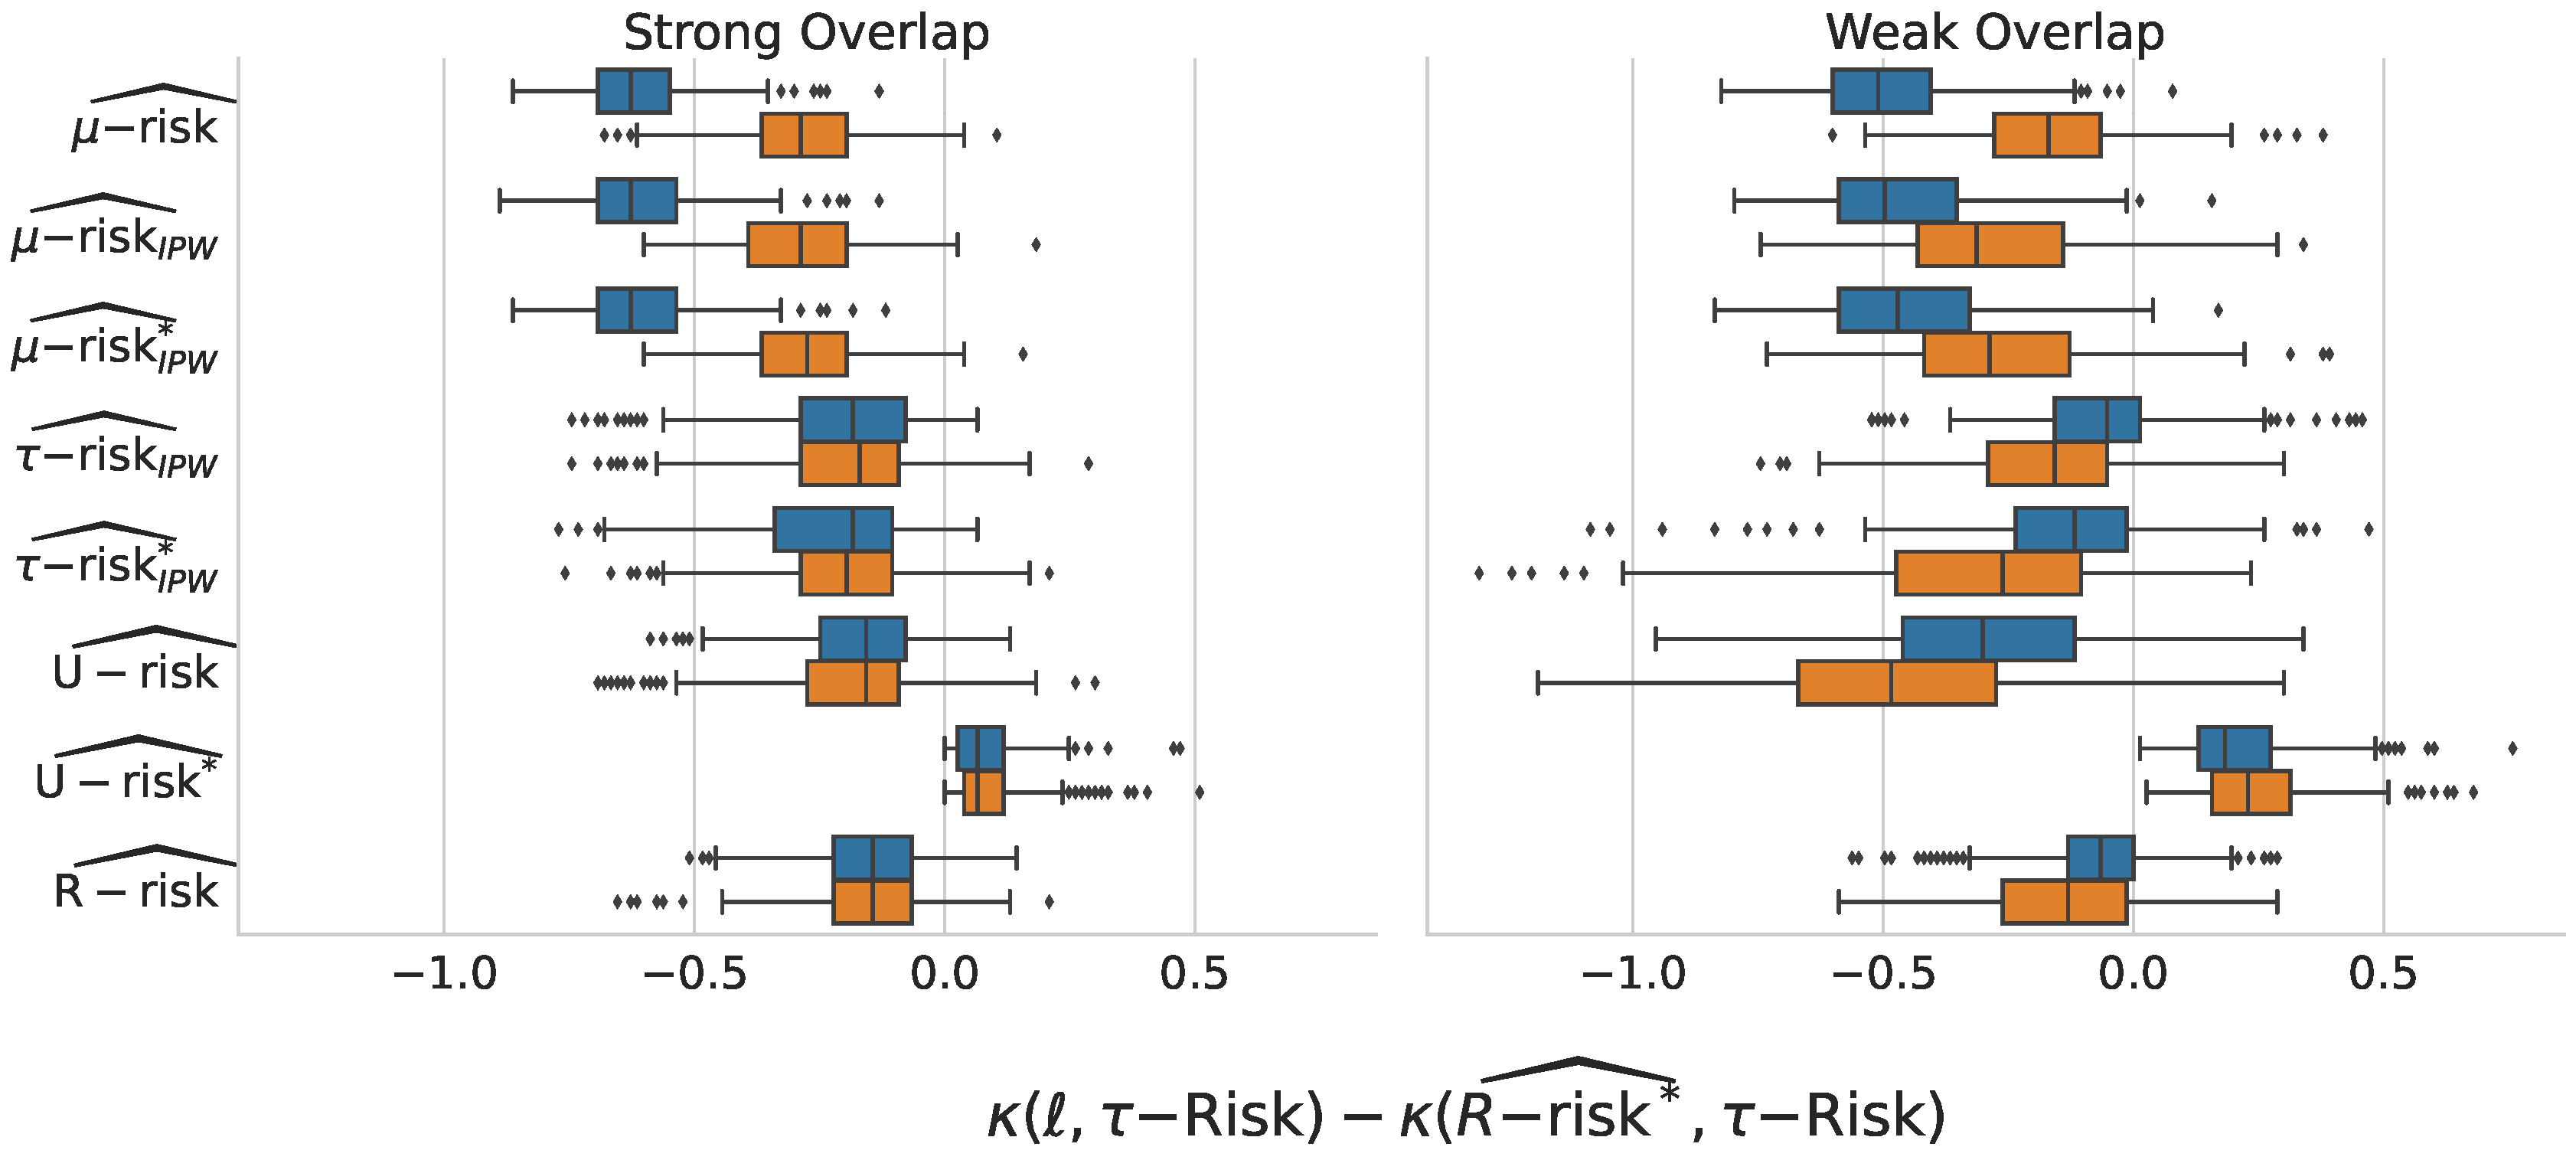
\includegraphics[width=1\textwidth]{_3_procedure_Twins_N11984__ref_metric_oracle_r_risk_training_procedure.pdf}
            \label{fig:experiments:procedures_comparison:twins}
        \end{subfigure}
        \hfill
        \caption{Results are similar between the \textcolor{MidnightBlue}{Shared
                nuisances/candidate set} and
            the \textcolor{RedOrange}{Separated nuisances set} procedure. The
            experience has not been run on the full metrics for Caussim due to computation costs.}\label
        {apd:fig:procedures_comparison_all_metrics}
    \end{figure}

    \paragraph{Figure \ref{apd:fig:all_datasets_overlap_effect} Low population
        overlap hinders model selection for all metrics}



    \begin{figure}
        \centering
        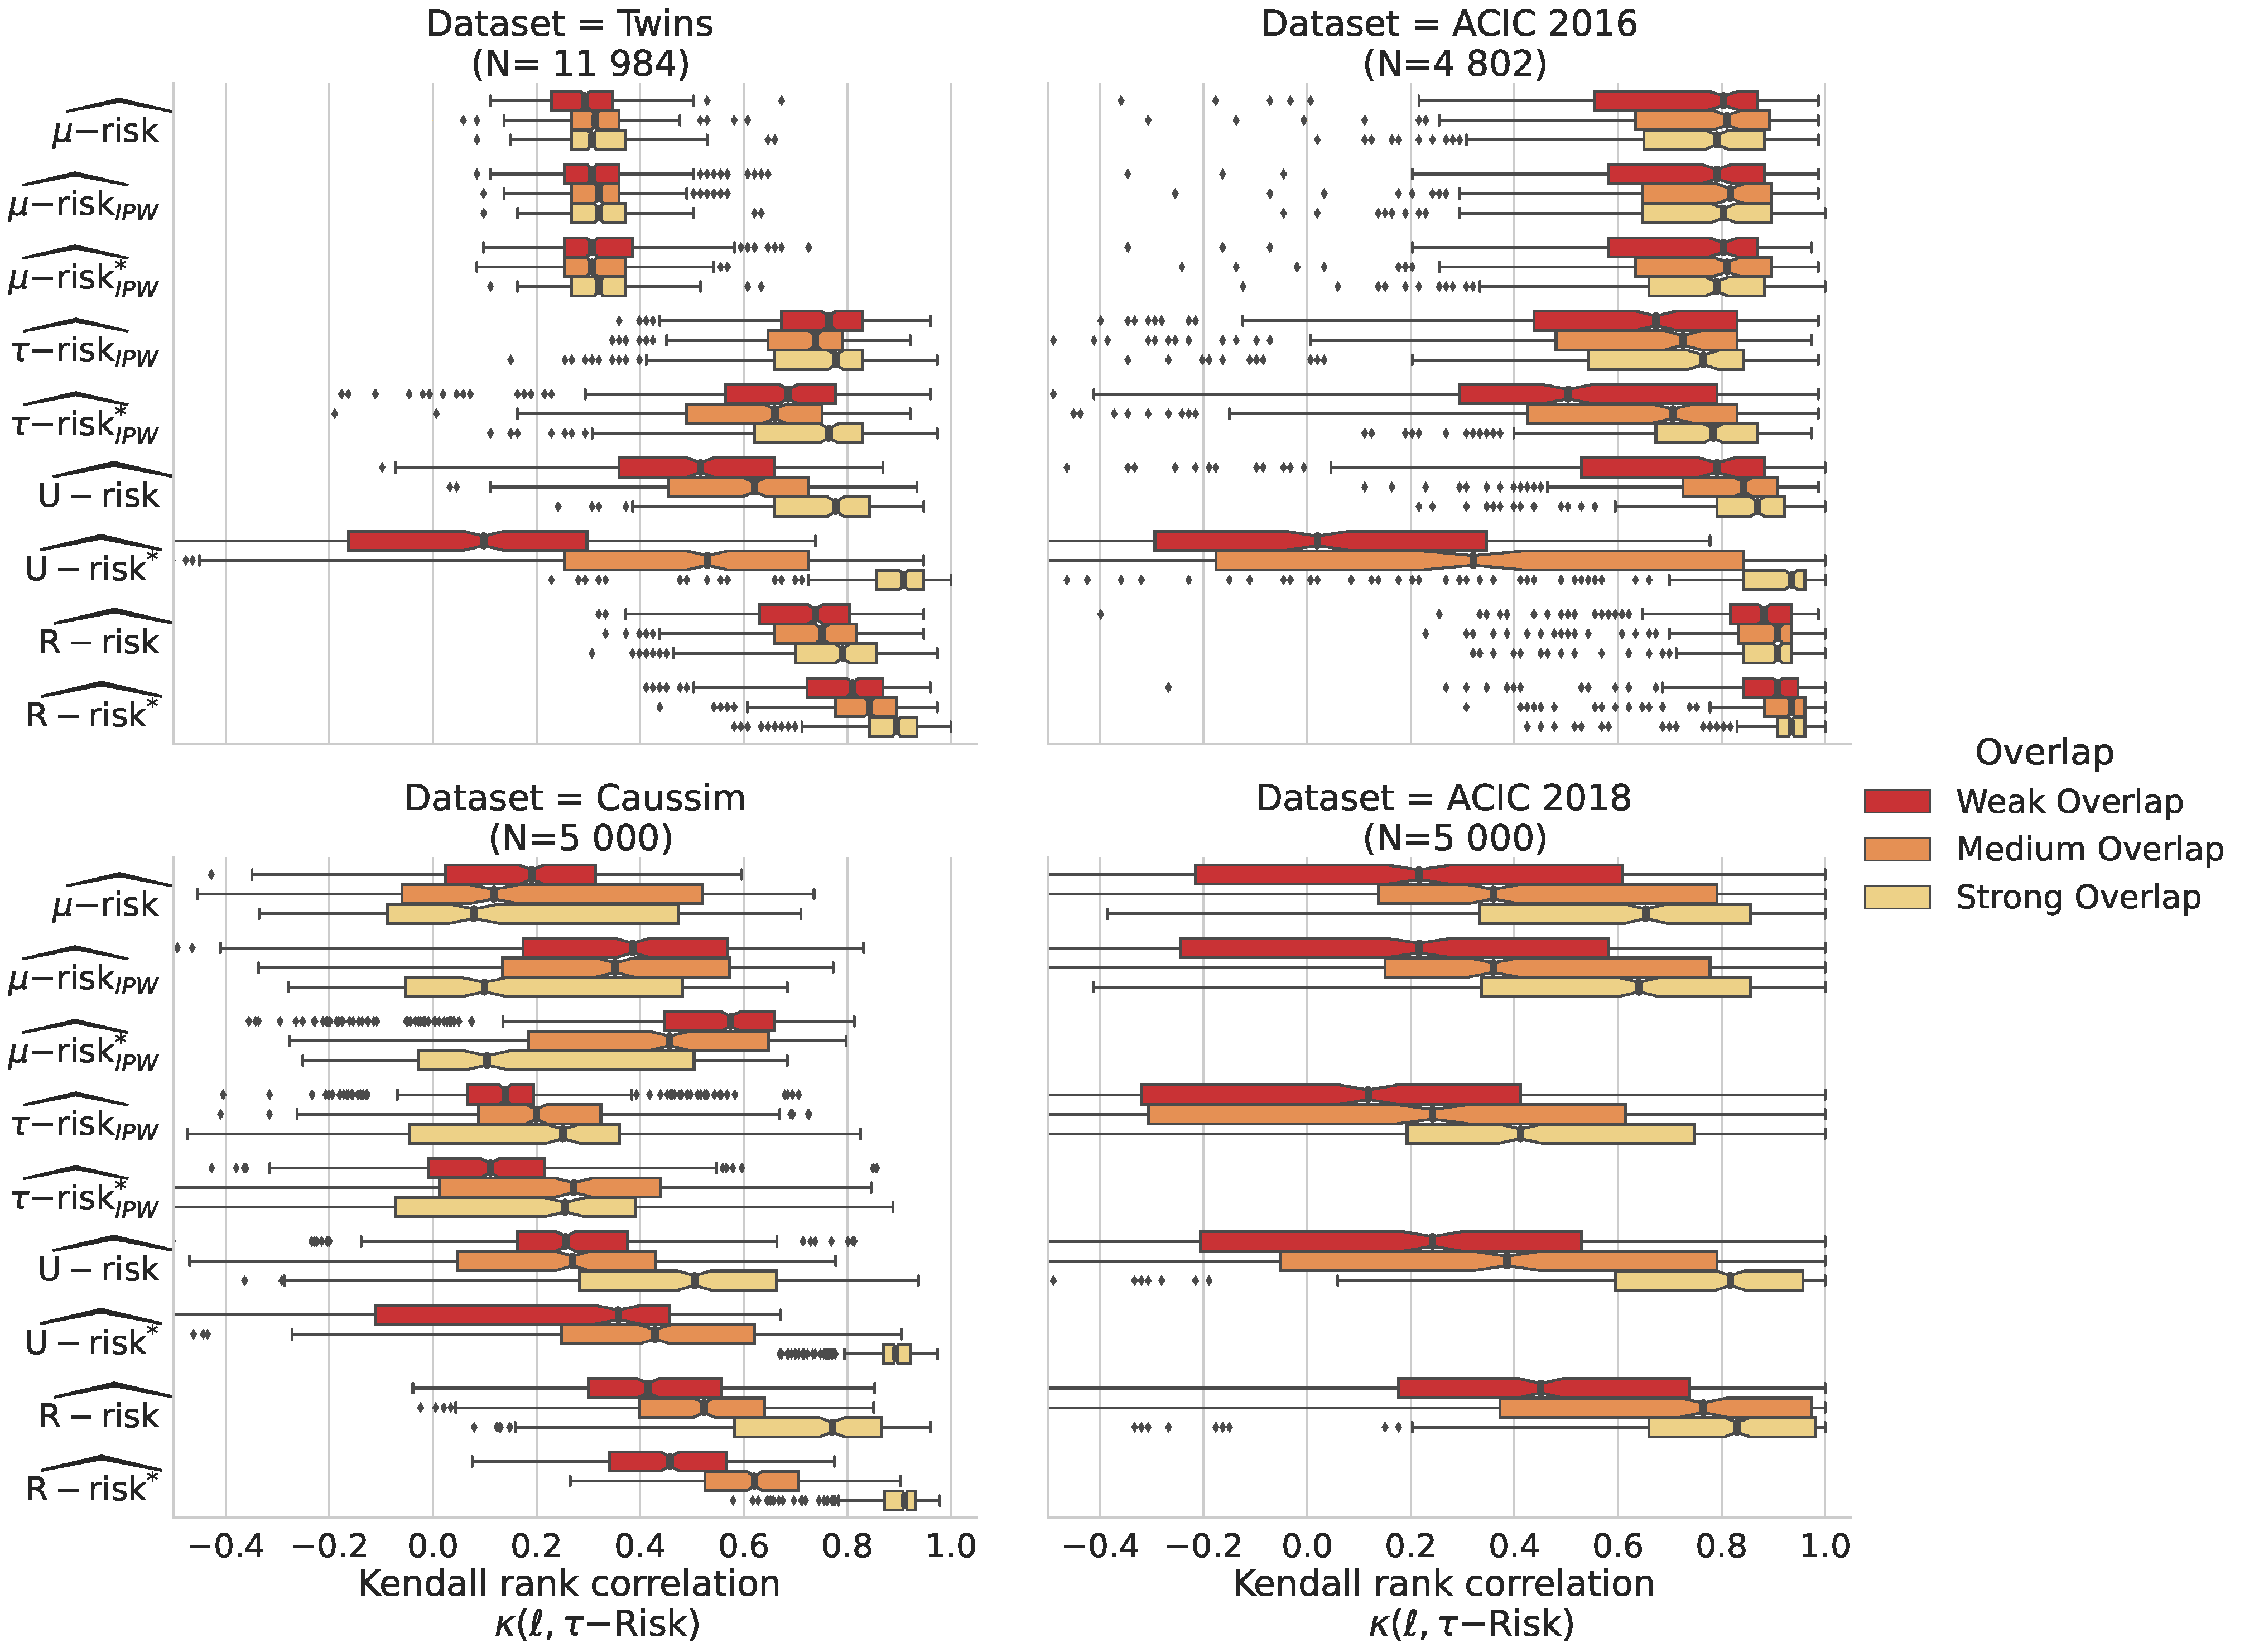
\includegraphics[width=\textwidth]{_2_overlap_influence_overlap_by_bin_comparaison_kendall_by_Dataset.pdf}
        \hfill
        \caption{\textbf{Low population overlap hinders causal model selection for all
                metrics}:
            Kendall's $\tau$ agreement with $\tau\text{-risk}$. Strong, medium and Weak overlap
            correspond
            to the tertiles of the overlap distribution measured with Normalized Total
            Varation eq. \ref{eq:ntv}.}\label{apd:fig:all_datasets_overlap_effect}
    \end{figure}


    \paragraph{Figure \ref{apd:fig:nuisances_comparison} - Stacked models for the nuisances is more efficient}
    For each metrics the benefit of
    using a stacked model of linear and boosting estimators for nuisances compared
    to a linear model. The evaluation measure is Kendall's tau relative to the
    oracle $R\text{-risk}^{\star}$ to have a stable reference between exepriments.
    Thus, we do not include in this analysis the ACIC 2018 dataset since
    $R\text{-risk}^{\star}$ is not available due to the lack of the true propensity
    score.

    \begin{figure}
        \begin{subfigure}[b]{0.49\textwidth}
            \centering
            \caption{\textbf{Twins}}
            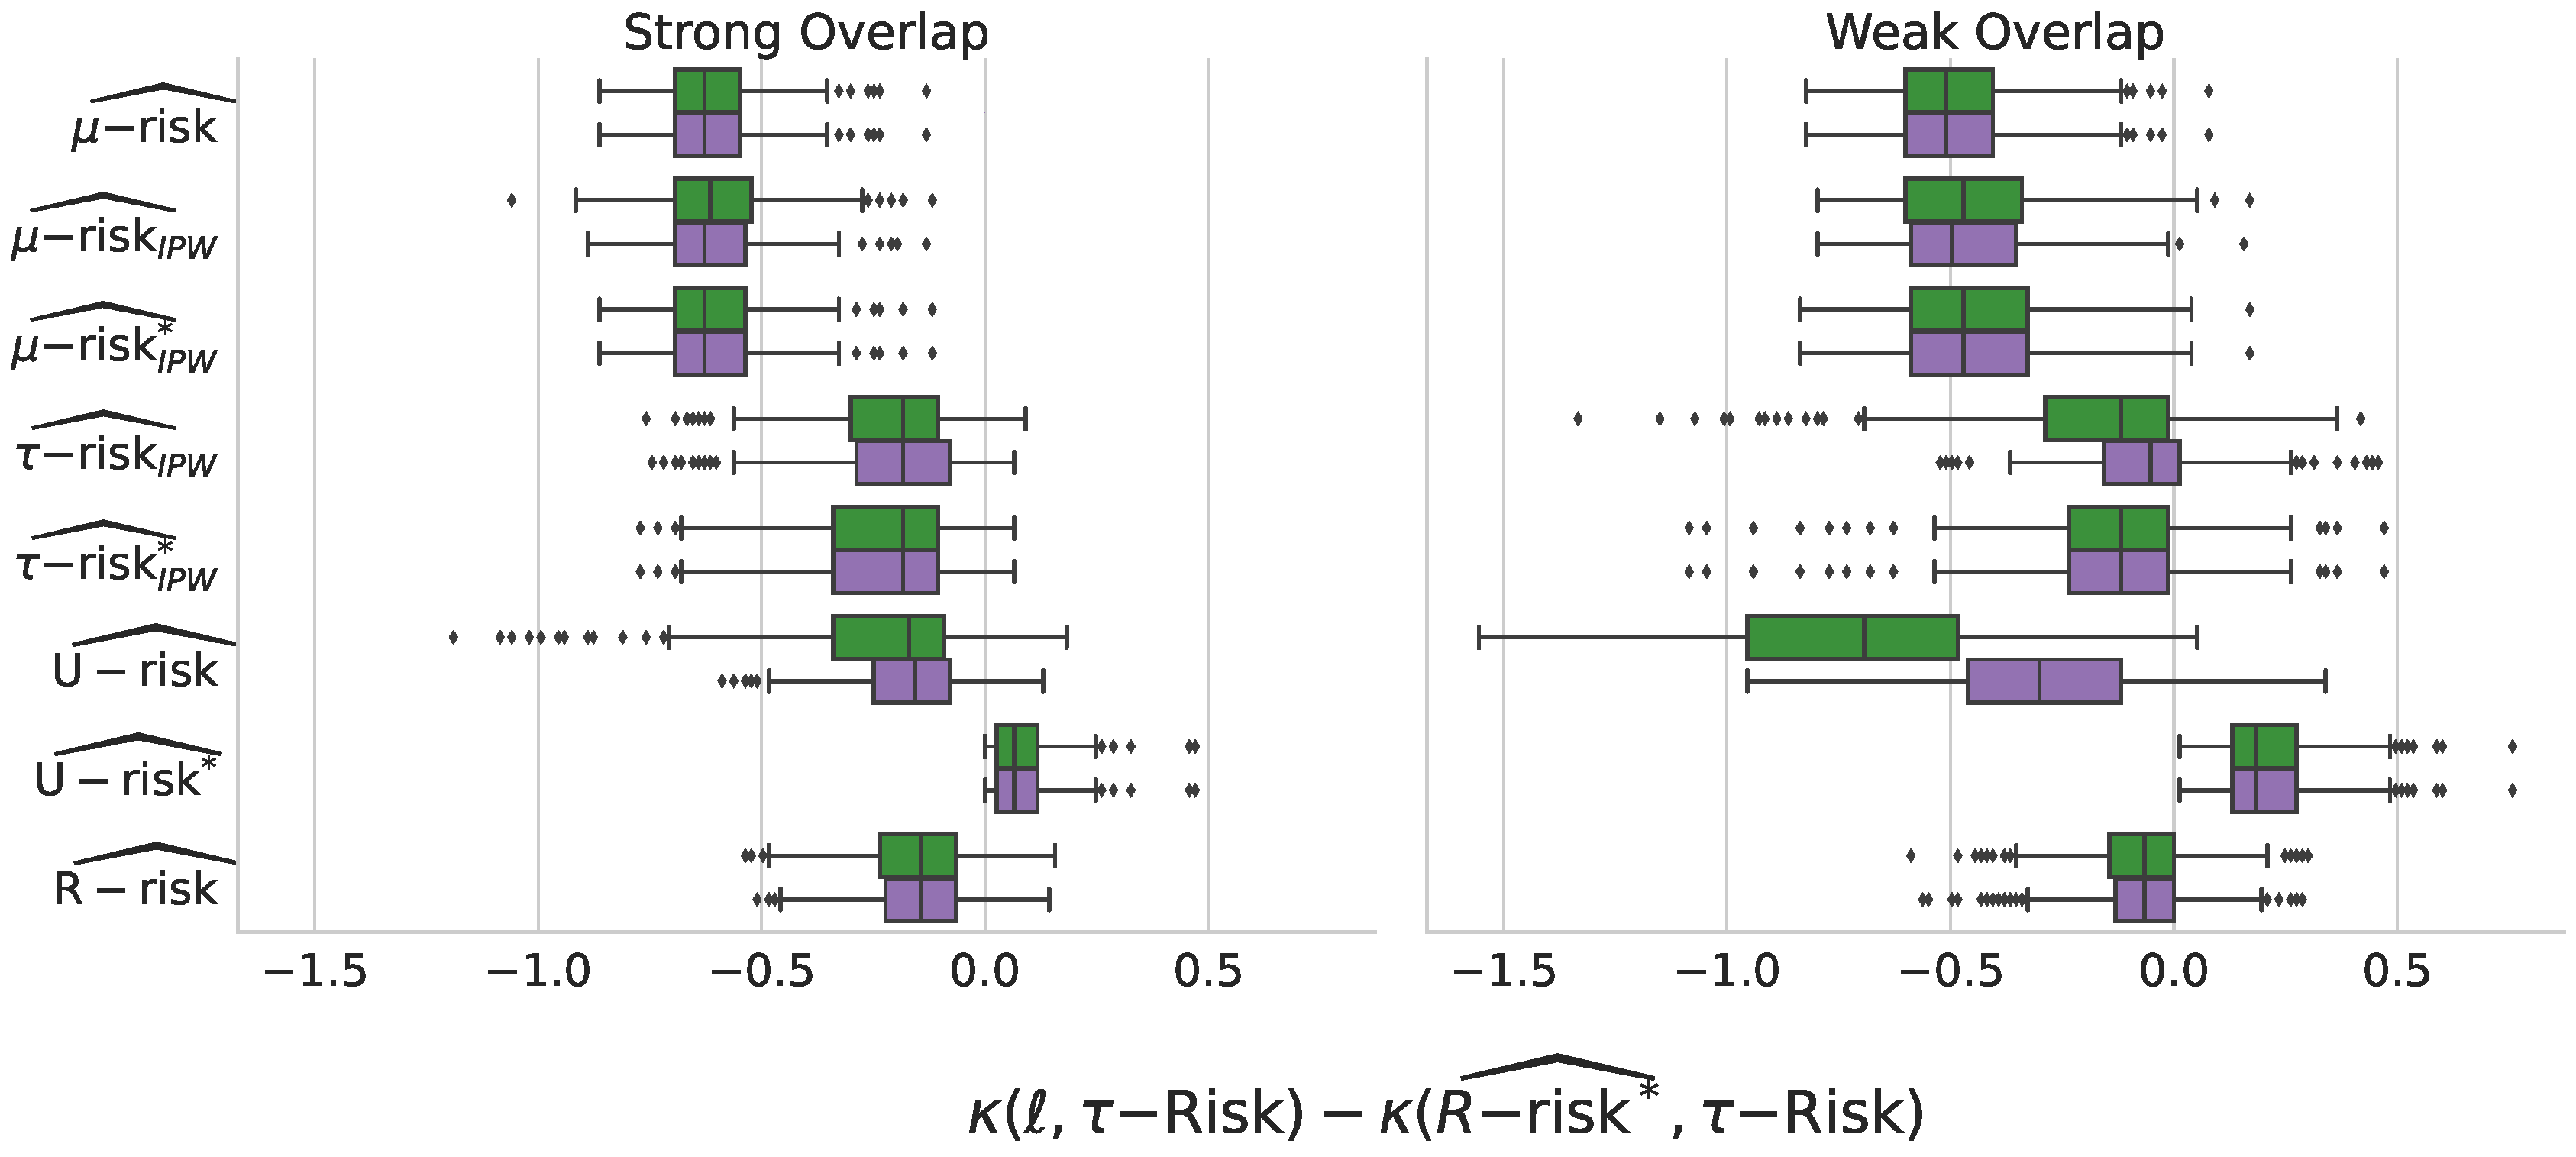
\includegraphics[width=1\textwidth]{_4_nuisance_models_Twins_N11984__ref_metric_oracle_r_risk_nuisance_models.pdf}
            \label{fig:experiments:nuisance_comparison:twins}
        \end{subfigure}
        \hfill
        \begin{subfigure}[b]{0.49\textwidth}
            \centering
            \caption{\textbf{Twins downsampled}}
            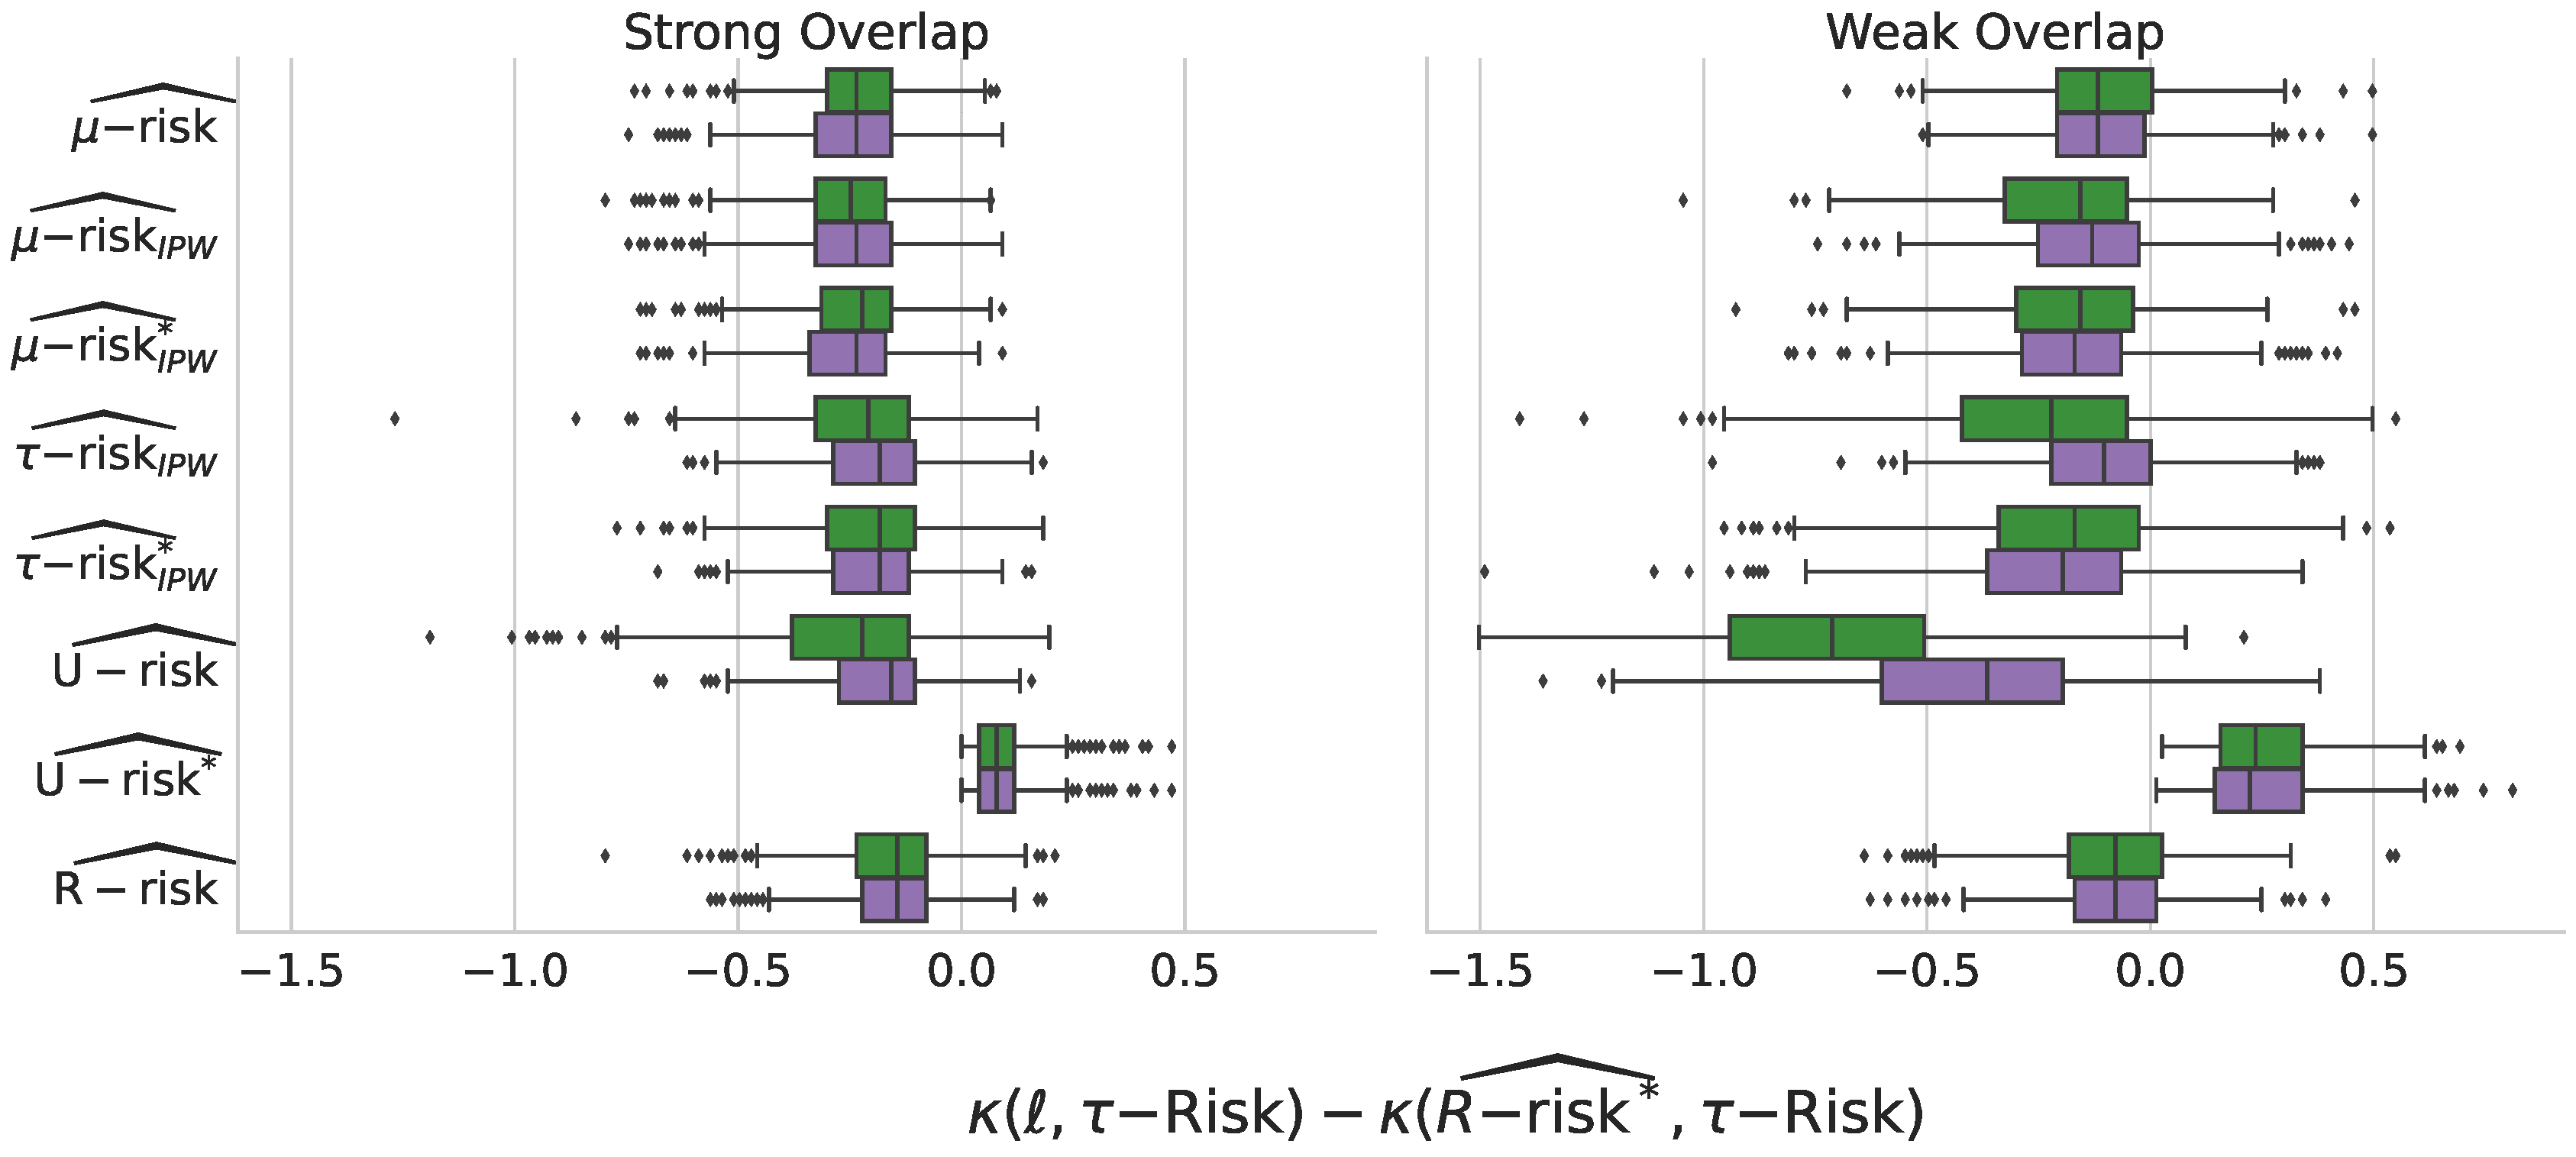
\includegraphics[width=1\textwidth]{_4_nuisance_models_Twinsdownsampled_N4794__ref_metric_oracle_r_risk_nuisance_models.pdf}
            \label{fig:experiments:nuisance_comparison:twins_ds}
        \end{subfigure}
        \hfill
        \begin{subfigure}[b]{0.49\textwidth}
            %\centering
            \caption{\textbf{Caussim}}
            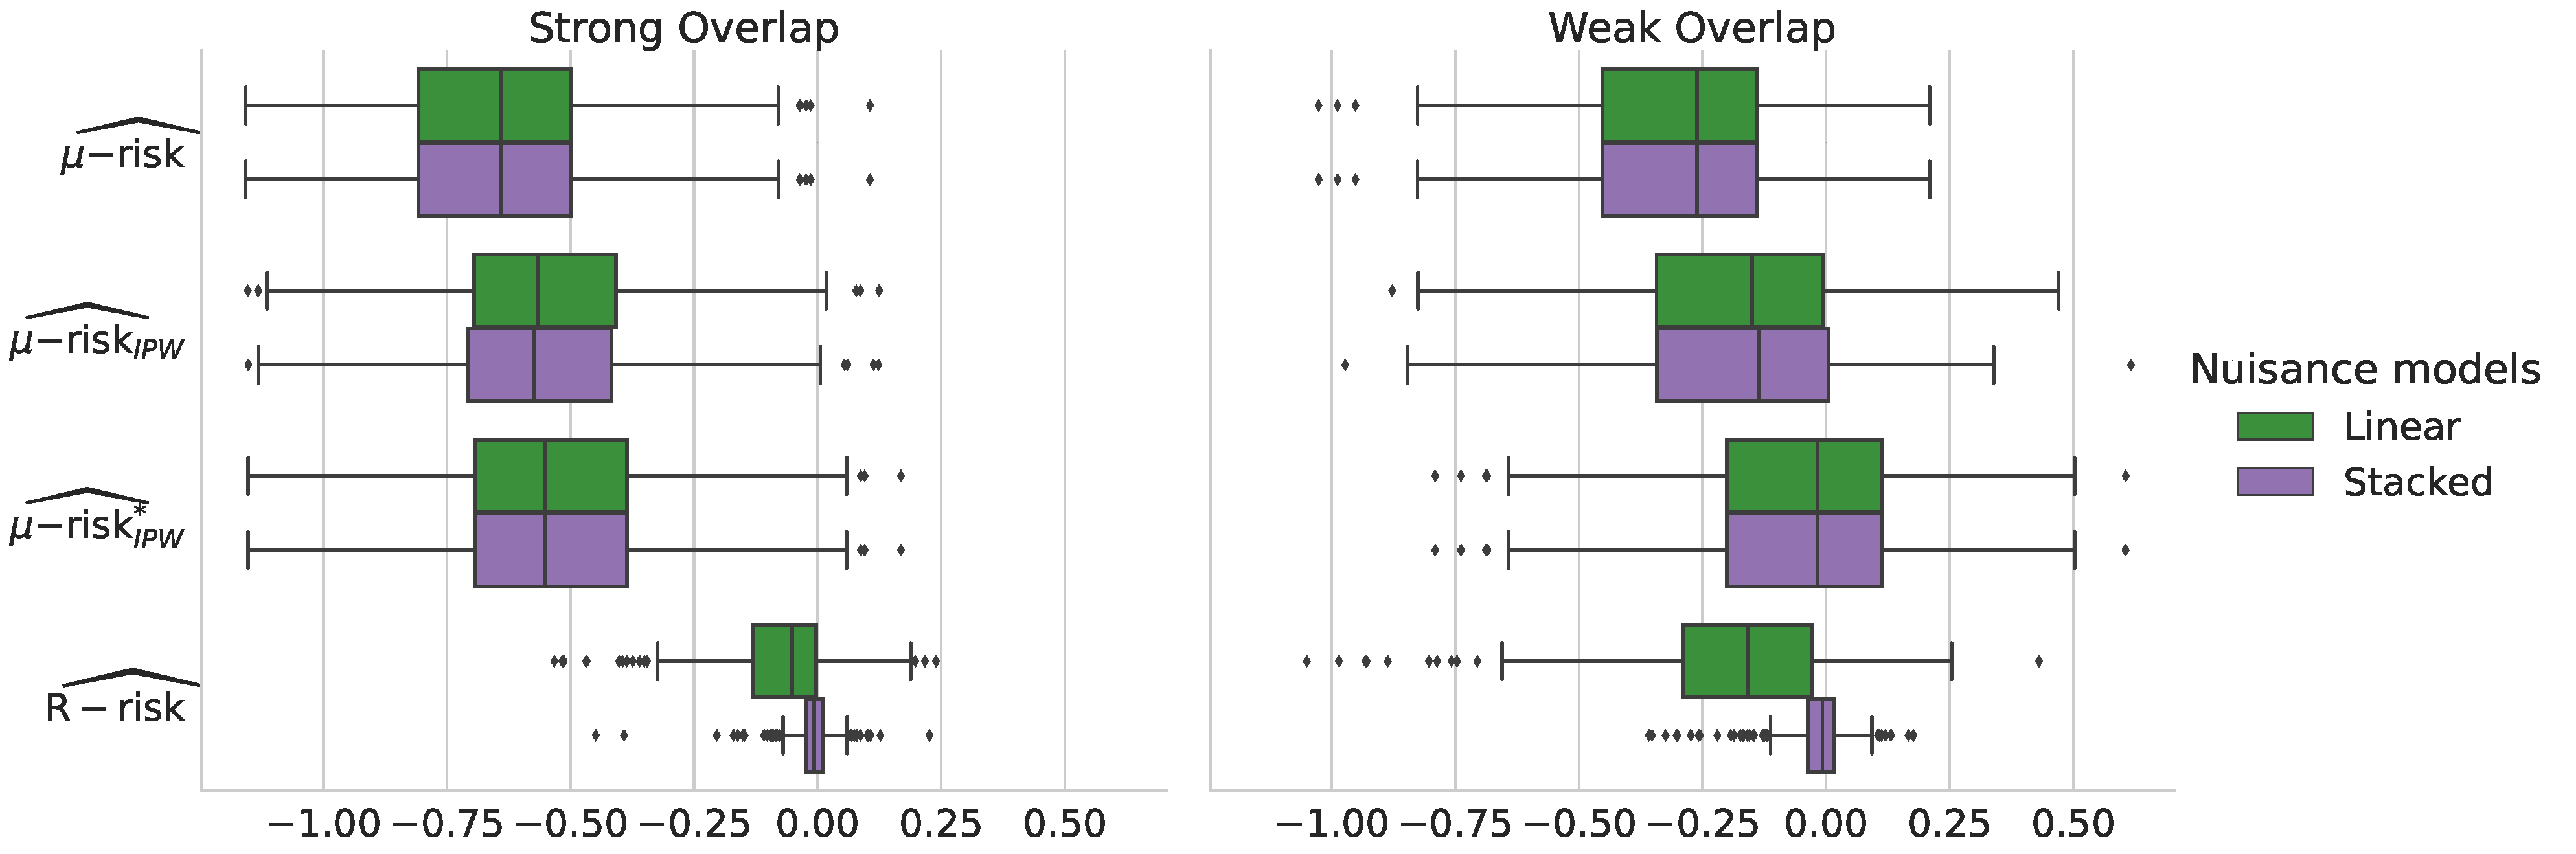
\includegraphics[width=1.15\textwidth]{_4_nuisance_models_Caussim_N5000__ref_metric_oracle_r_risk_nuisance_models.pdf}
            \label{fig:experiments:nuisance_comparison:caussim}
        \end{subfigure}
        \hfill
        \begin{subfigure}[b]{0.49\textwidth}
            \centering
            \caption{\textbf{ACIC 2016}}
            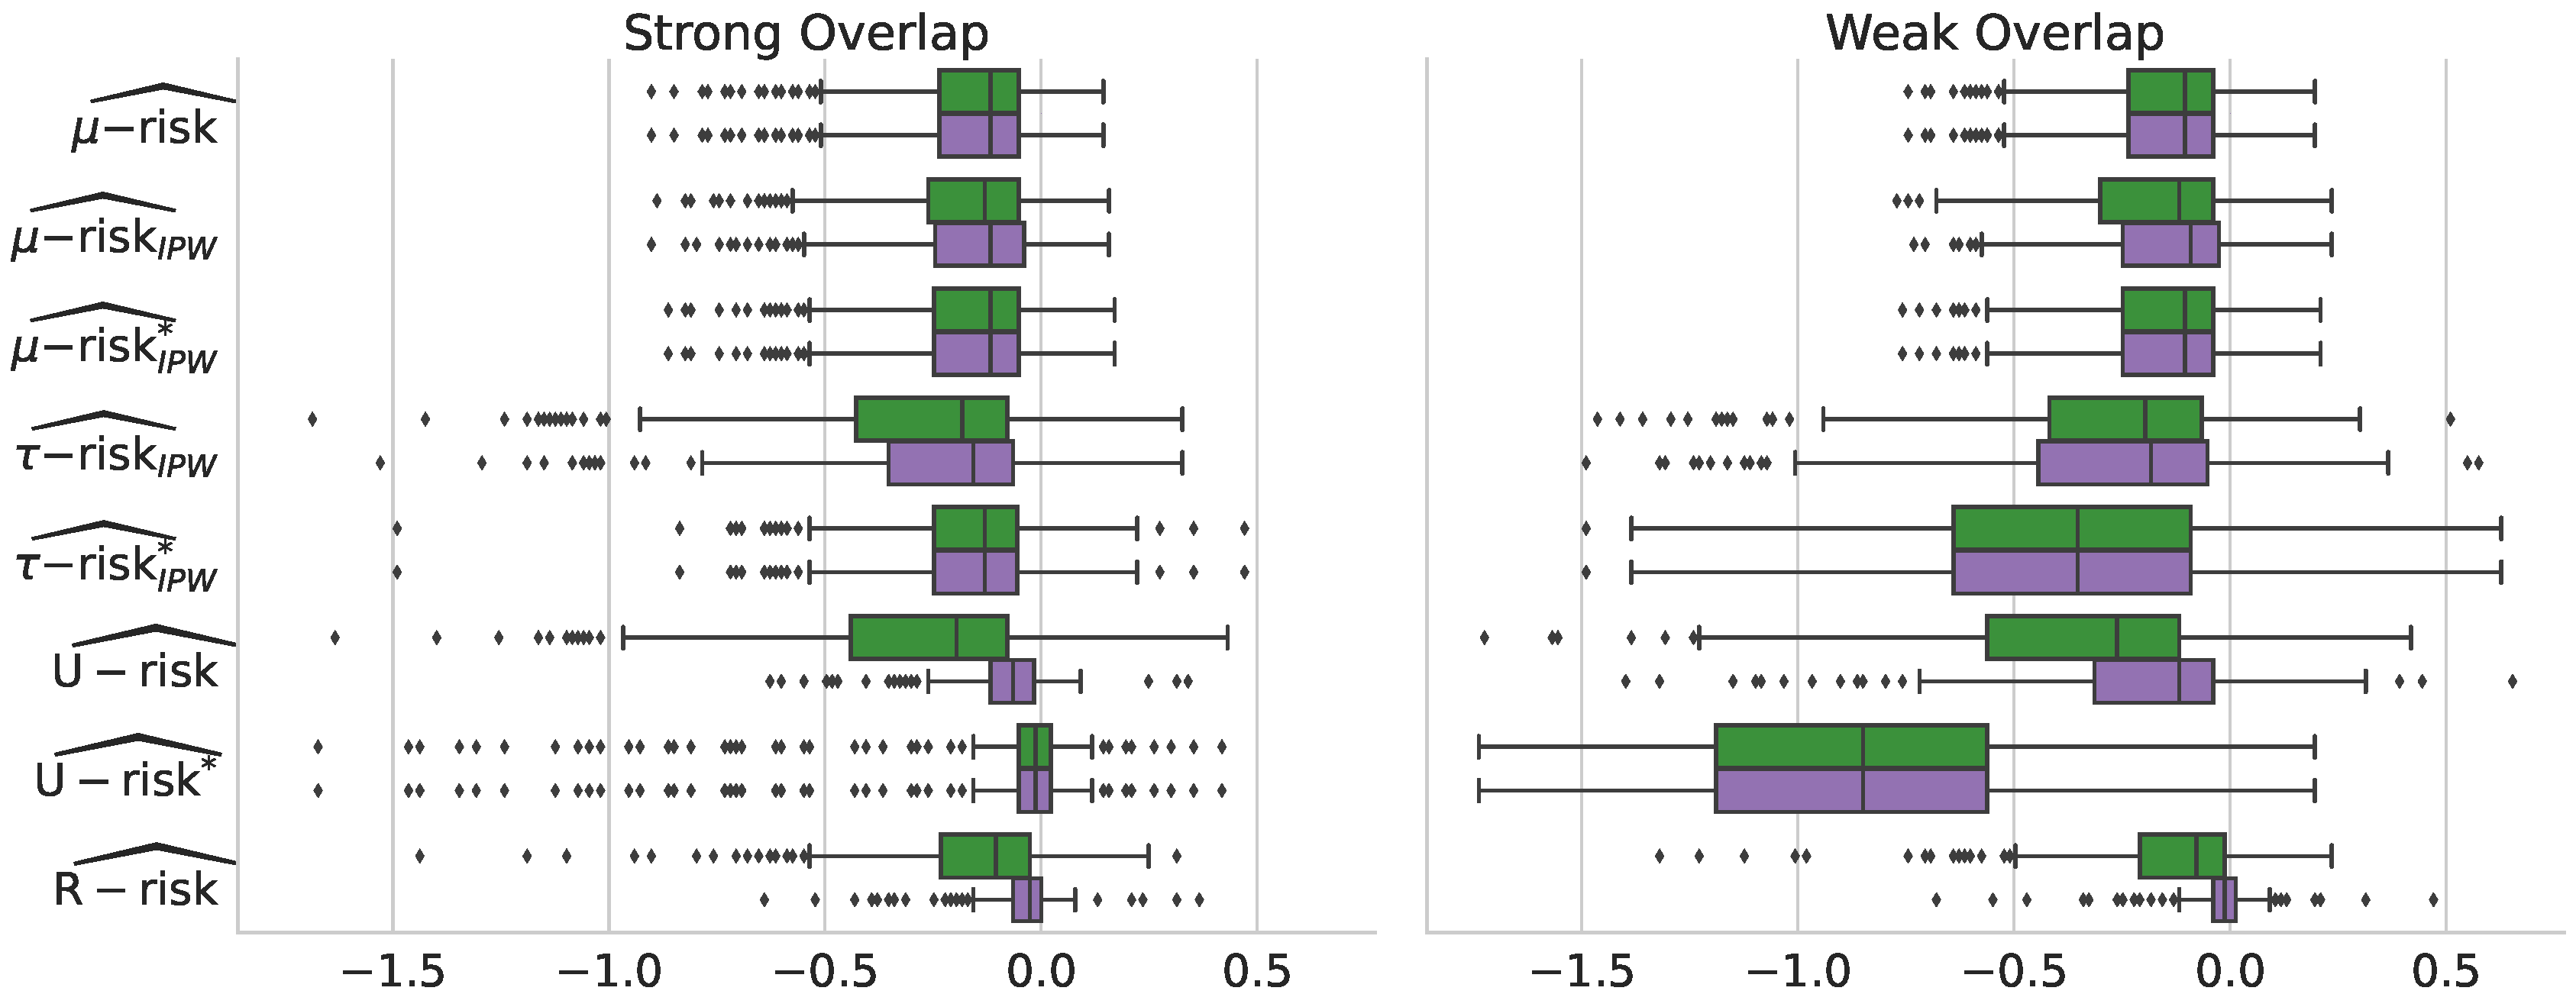
\includegraphics[width=1\textwidth]{_4_nuisance_models_ACIC2016_N4802__ref_metric_oracle_r_risk_nuisance_models.pdf}
            \label{fig:experiments:nuisance_comparison:acic_2016}
        \end{subfigure}
        \hfill
        \caption{Learning the nuisances with \textcolor{DarkOrchid}{stacked models} (linear and
            gradient boosting) is important for successful model selection with R-risk.
            For Twins dataset, there is no improvement for \textcolor{DarkOrchid}{stacked models} compared to
            \textcolor{ForestGreen}{linear models} because of the linearity of the propensity model.}\label
        {apd:fig:nuisances_comparison}
    \end{figure}

    \paragraph{Figure \ref{apd:fig:nuisances_comparison_twins} - Flexible models are performant in recovering nuisances even
        in linear setups}

    \begin{figure}
        \centering
        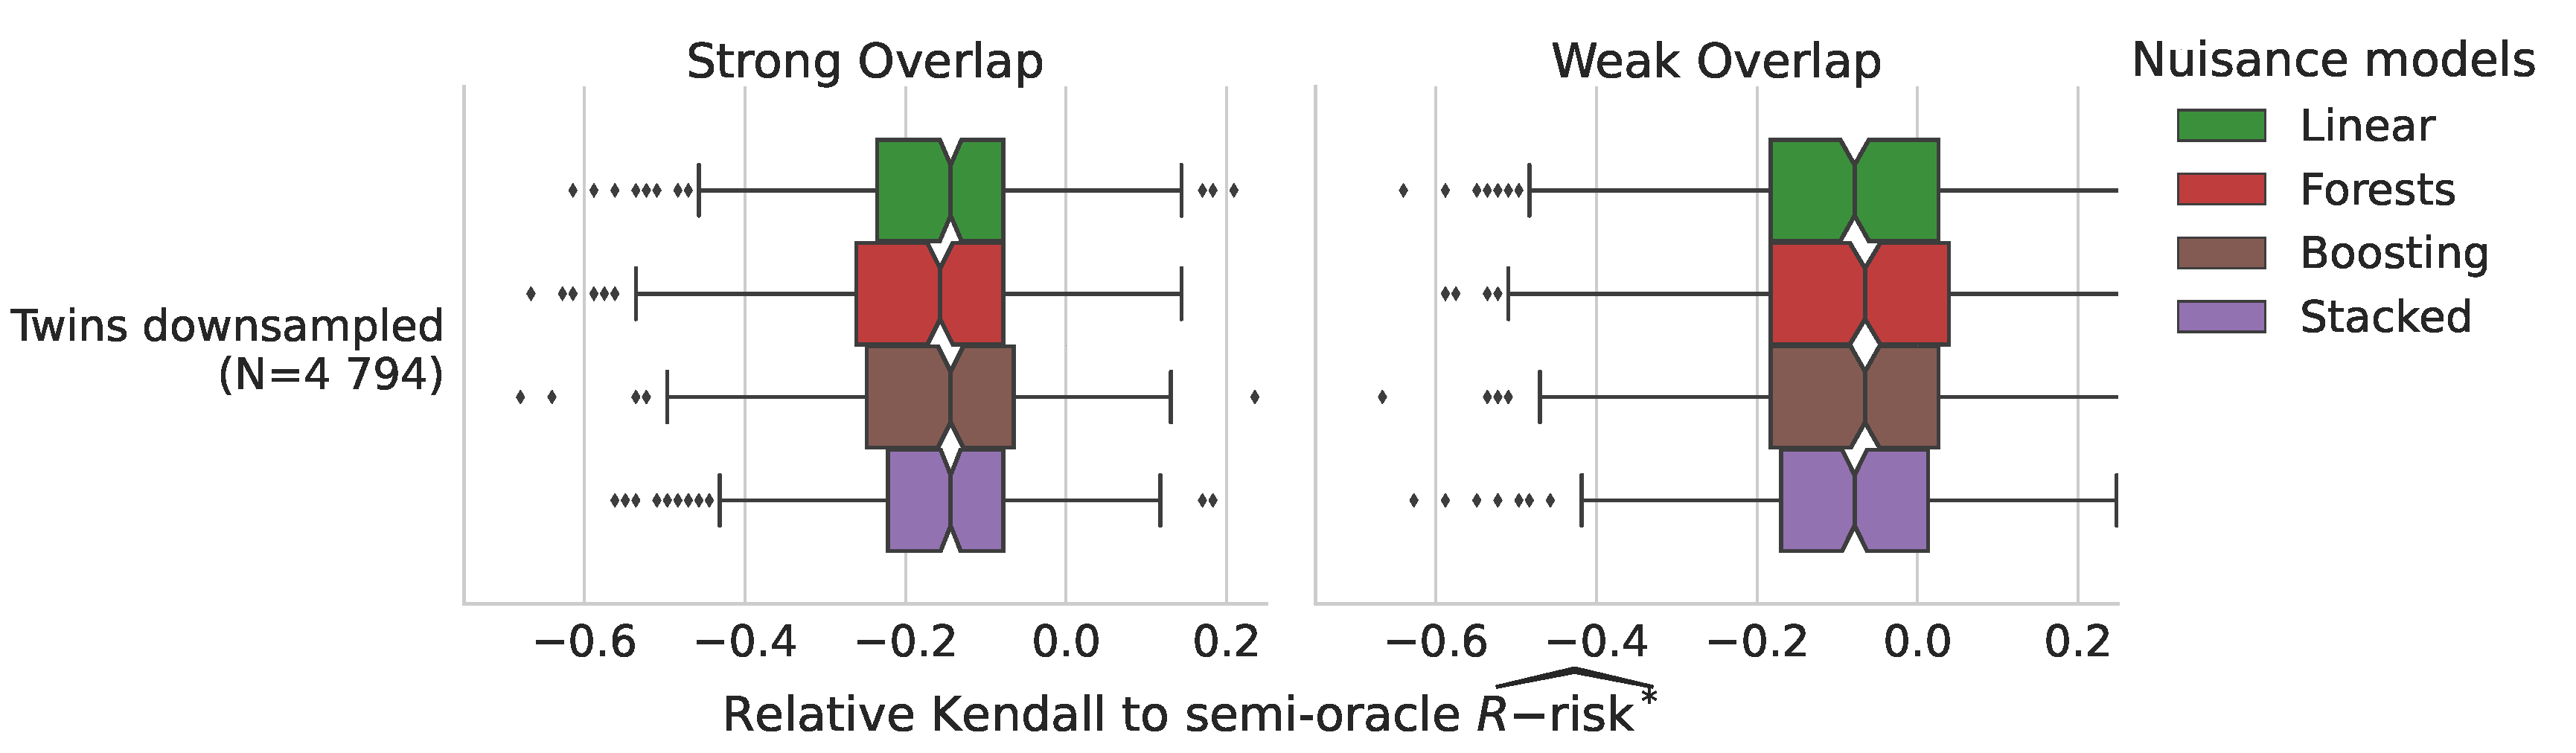
\includegraphics[width=\textwidth]{_4_nuisance_models_r_risk_only_twins_nuisances.pdf}
        \hfill
        \caption{\textbf{Flexible models are performant in recovering nuisances
                in the downsampled Twins dataset.} The propensity score is linear in this
            setup, making it particularly challenging for flexible models compared to
            linear methods.}\label{apd:fig:nuisances_comparison_twins}
    \end{figure}


    \paragraph{Selecting different seeds and parameters is crucial to draw
        conclusions}\label{apd:results:seed_effect}

    One strength of our study is the various number of different simulated and
    semi-simulated datasets. We are convinced that the usual practice of using only
    a small number of generation processes does not allow to draw statistically
    significant conclusions.

    Figure \ref{apd:results:fig:seed_effect} illustrate the dependence of the
    results on the generation process for caussim simulations. We highlighted the
    different trajectories induced by three different seeds for data generation and
    three different treatment ratio instead of 1000 different seeds. The result
    curves are relatively stable from one setup to another for $R{-risk}$, but vary
    strongly for $\mu\text{-risk}$ and $\mu\text{-risk}_{IPW}$.

    \begin{figure}
        \centering
        \caption{Kendall correlation coefficients for each causal metric. Each (color,
            shape) pair indicates a different (treatment ratio, seed) of the generation
            process.}\label {apd:results:fig:seed_effect}
        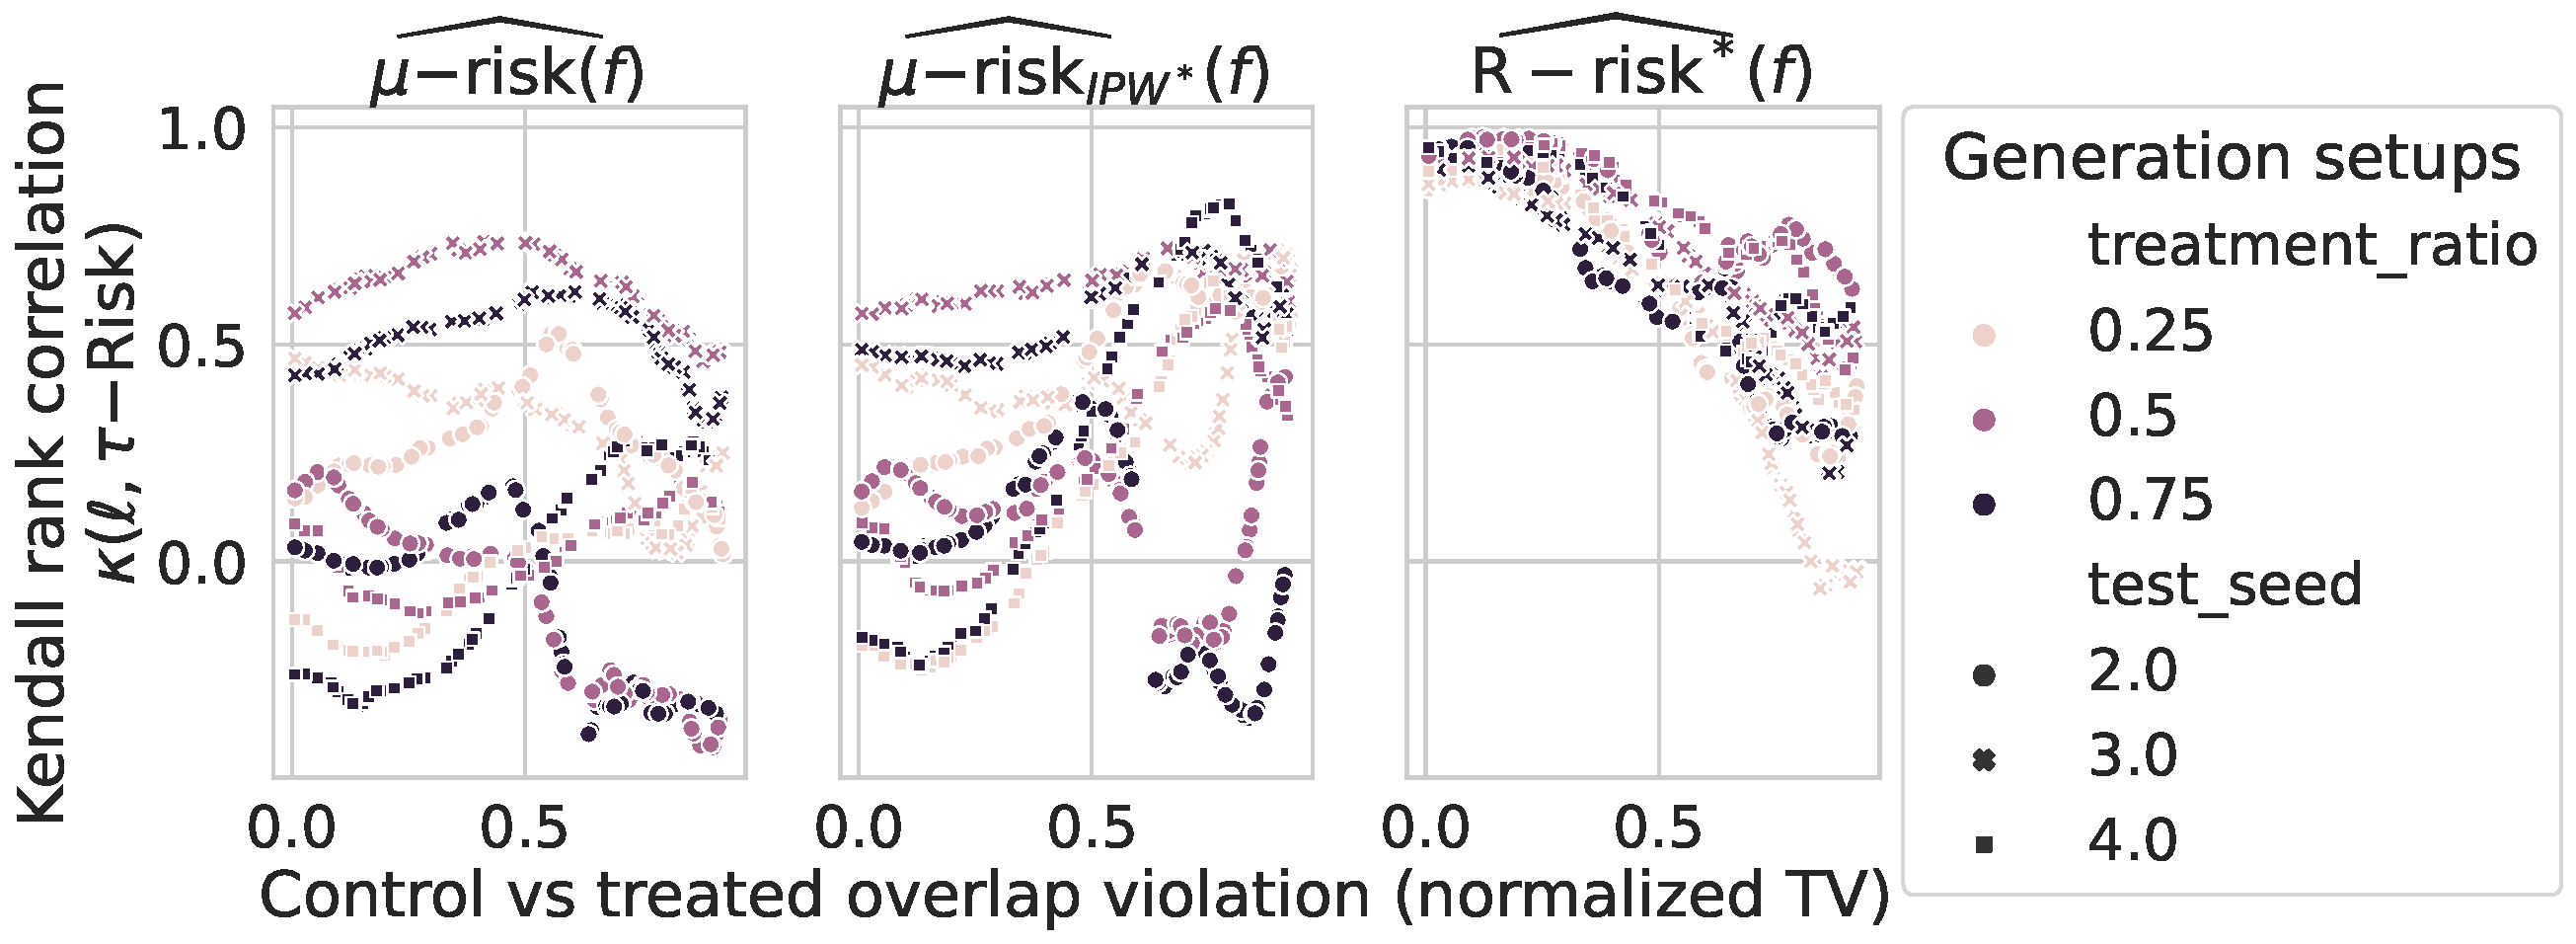
\includegraphics[width=\linewidth]{caussim_seed_effect.pdf}
    \end{figure}

    \FloatBarrier

    \section{Data split choices}\label{apd:results:data_split}

    \subsection{Use 90\% of the data to estimate outcome models, 10\% to
        select them}

    The analyst faces a compromise: given a finite
    data sample, should she allocate more data to estimate the outcome model,
    thus improving the quality of the outcome model but leaving
    little data for model selection. Or, she could choose a bigger test set for
    model selection and effect estimation. For causal model selection, there
    is no established practice (as reviewed in \ref{apd:results:k_fold_choices}).

    We investigate such tradeoff varying the ratio between train and test
    data size. For this, we first split out 30\% of the data as a holdout set
    $\mathcal{V}$ on which we use the oracle response functions to derive
    silver-standard estimates of causal quantities. We then
    use the standard estimation procedure on the remaining 70\% of the data,
    splitting it into train $\mathcal{T}$ and test $\mathcal{S}$ of varying
    sizes. We finally measure the error between this estimate and the
    silver standard.

    We consider two different analytic goals: estimating a average
    treatment effect --a single number used for policy making-- and a
    CATE --a full model of the treatment effect as a function of covariates
    $X$. Given that the latter is a much more complex object than the former,
    the optimal train/test ratio might vary. To measure errors, we use for
    the ATE the relative absolute ATE bias between the ATE computed with the
    selected outcome model on the test set, and the true ATE as evaluated on
    the holdout set $\mathcal{V}$. For the CATE, we compare the
    $\tau\text{-risk}$
    of the best selected model applied on the holdout set $\mathcal{V}$. We explore this trade-off for the ACIC 2016 dataset and the R-risk.

    \begin{figure}[!t]
        \begin{minipage}{.5\textwidth}
            \centerline{\textbf{a) CATE estimation error}}
            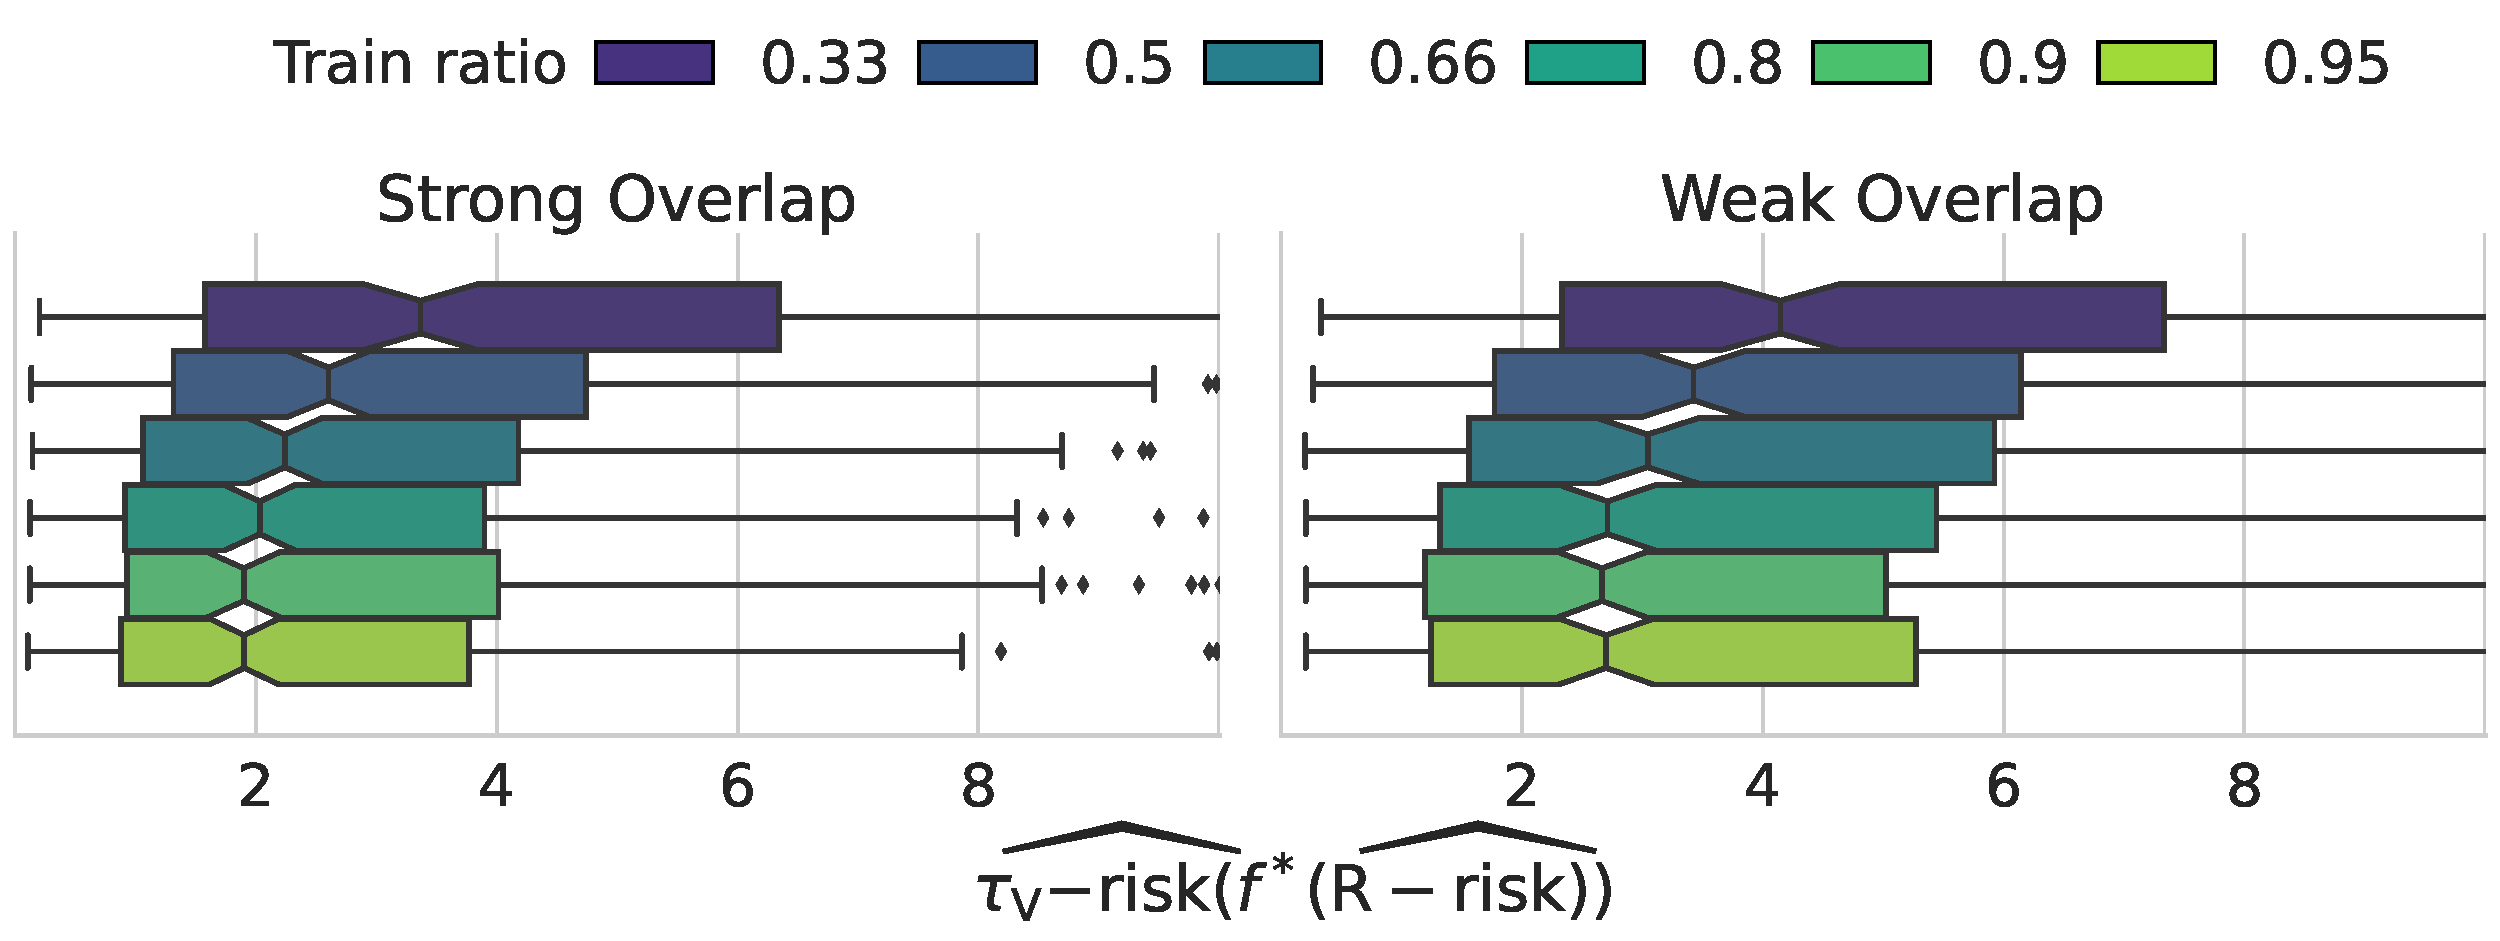
\includegraphics[width=\linewidth]{_5_train_size_evaluated_metric_r_risk__evaluation_validation_tau_risk__best_tau_norm__False_norm_False__acic16_twocols.pdf}
        \end{minipage}
        %\hspace{0.3\textwidth}
        \begin{minipage}{.5\textwidth}
            \centerline{\textbf{b) ATE estimation error}}
            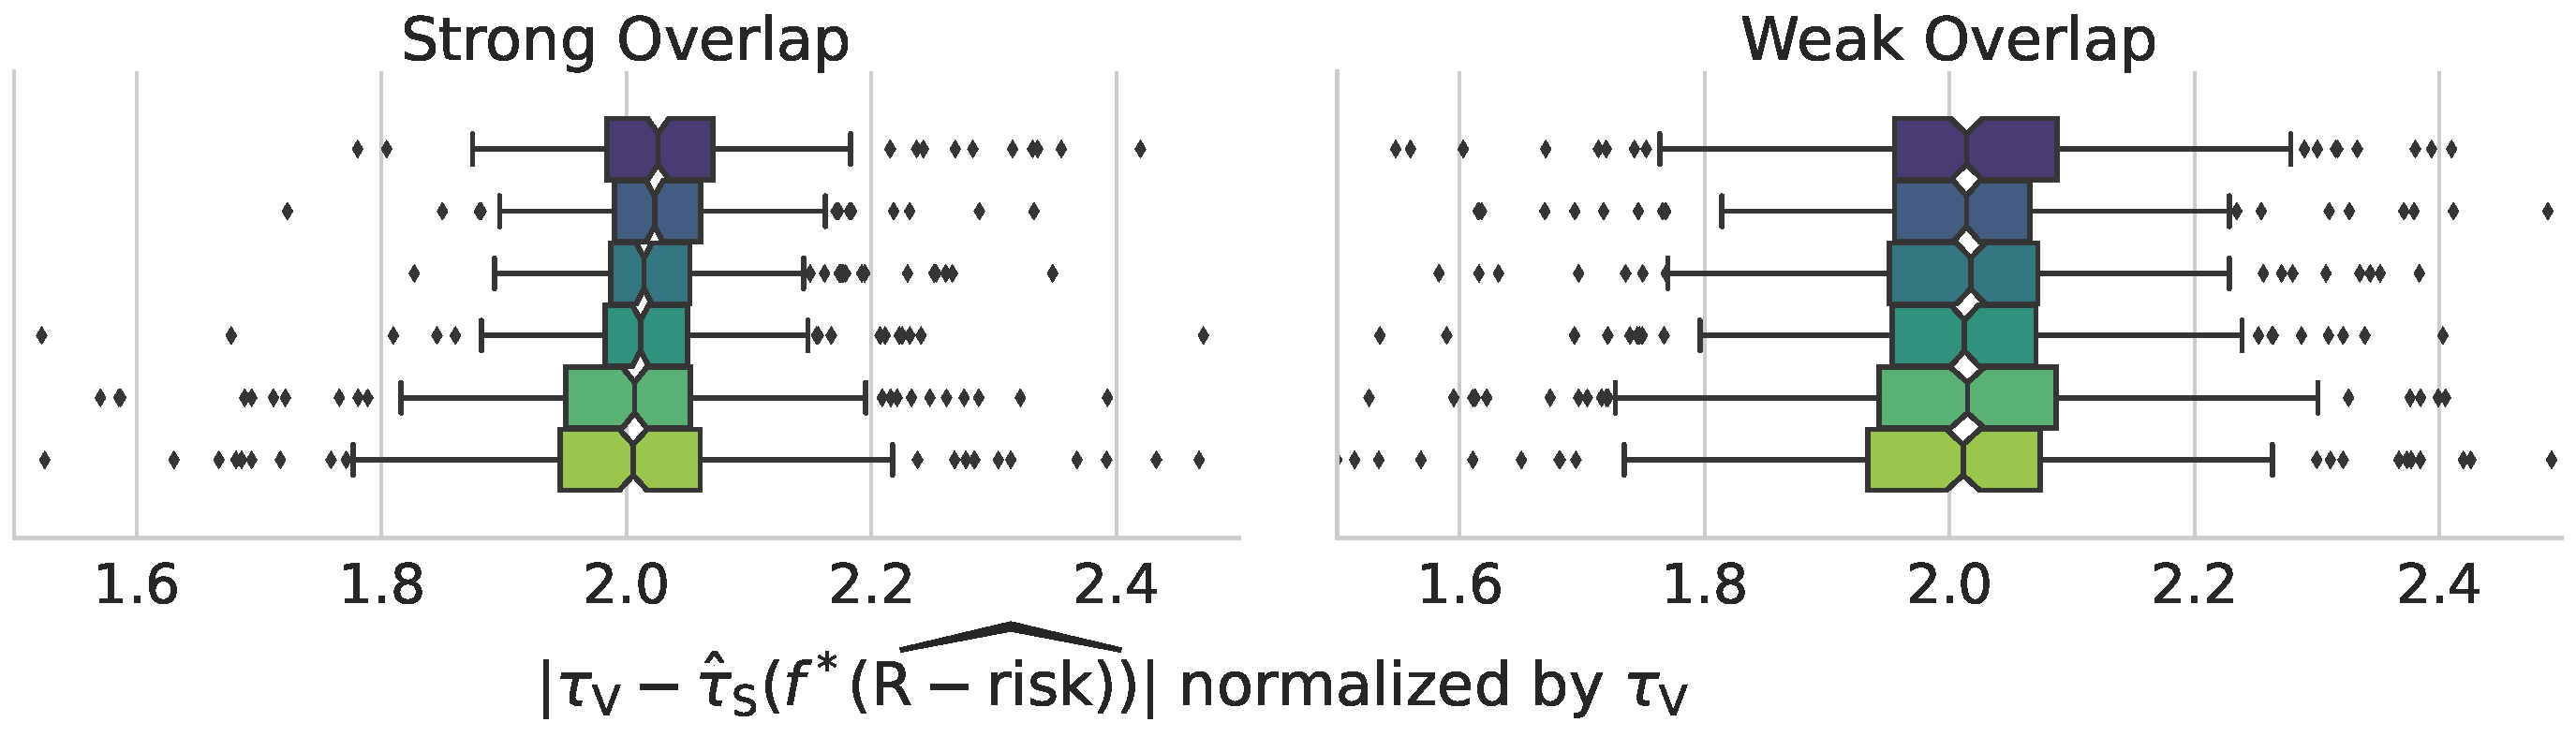
\includegraphics[width=\linewidth]{_5_train_size_evaluated_metric_r_risk__evaluation_validation_test_abs_bias_ate__best_tau_norm__False_norm_True__acic16_twocols.pdf}
        \end{minipage}%
        \caption{\textbf{a) For CATE, a train/test ratio of 0.9/0.1 appears a good
                trade-off.} b) For ATE, there is a small signal pointing also to
            0.9/0.1 (K=10).
            for ATE. Experiences on 10 replications of all 78 instances of the ACIC 2016
            data.}\label{fig:train_test_ratio}
    \end{figure}

    Figure \ref{fig:train_test_ratio} shows that a train/test ratio of
    0.9/0.1 (K=10) or 0.8/0.2 (K=5) appears best to estimate CATE and
    ATE.

    \subsection{Heterogeneity in practices for data split}\label{apd:results:k_fold_choices}

    Splitting the data is common when using machine learning for causal
    inference, but practices vary widely in terms of the fraction of data to
    allocate to train models, outcomes and nuisances, and to evaluate them.

    Before even model selection, data splitting is often required for
    estimation of the treatment effect, ATE or CATE, for instance to compute
    the nuisances required to optimize the outcome model (as the
    $R\text{-risk}$, Definition \ref{def:r_risk}).
    %
    The most frequent choice is use 80\% of the data to fit the models,
    and 20\% to evaluate them.
    %
    For instance, for CATE estimation, the R-learner has been introduced using K-folds with K = 5
    and K = 10: 80\% of the data (4 folds) to train the nuisances and the remaining
    fold to minimize the corresponding R-loss \cite{nie_quasioracle_2017}.
    Yet, it has been implemented with K=5 in causallib
    \cite{causalevaluations} or K=3 in econML \cite{econml}.
    Likewise, for ATE estimation, \cite{chernozhukov_double_2018}
    introduce doubly-robust machine learning,
    recommending K=5 based on an empirical comparison K=2. However,
    subsequent works use doubly robust ML with varying choices
    of K: \cite{loiseau_external_2022} use K=3, \cite{gao_assessment_2021} use
    K=2. In the econML implementation, K is set to 3 \cite{econml}.
    \cite{naimi2021challenges} evaluate various machine-learning approaches
    --including R-learners-- using K=5 and 10, drawing inspiration from the
    TMLE literature which sets
    K=5 in the TMLE package \cite{tmle_package_2012}.

    Causal model selection has been much less discussed. The only study that
    we are aware of, \cite{schuler_comparison_2018}, use a different data
    split: a 2-folds train/test procedure,
    training the nuisances on the first half of the data, and using the
    second half to estimate the $R\text{-risk}$ and select the best treatment
    effect model.

\end{appendices}

\section{Competing interests}
No competing interest is declared.

\section{Author contributions statement}

M.D. conceived and conducted the experiments, M.D. and G.V. analysed the results. M.D. and G.V. wrote and reviewed the manuscript.

\section{Acknowledgments}

We acknowledge fruitful discussions with Bénédicte Colnet.


\bibliography{biblio}
%\printbibliography


\end{document}
